\documentclass[twoside]{book}

% Packages required by doxygen
\usepackage{fixltx2e}
\usepackage{calc}
\usepackage{doxygen}
\usepackage[export]{adjustbox} % also loads graphicx
\usepackage{graphicx}
\usepackage[utf8]{inputenc}
\usepackage{makeidx}
\usepackage{multicol}
\usepackage{multirow}
\PassOptionsToPackage{warn}{textcomp}
\usepackage{textcomp}
\usepackage[nointegrals]{wasysym}
\usepackage[table]{xcolor}

% Font selection
\usepackage[T1]{fontenc}
\usepackage[scaled=.90]{helvet}
\usepackage{courier}
\usepackage{amssymb}
\usepackage{sectsty}
\renewcommand{\familydefault}{\sfdefault}
\allsectionsfont{%
  \fontseries{bc}\selectfont%
  \color{darkgray}%
}
\renewcommand{\DoxyLabelFont}{%
  \fontseries{bc}\selectfont%
  \color{darkgray}%
}
\newcommand{\+}{\discretionary{\mbox{\scriptsize$\hookleftarrow$}}{}{}}

% Page & text layout
\usepackage{geometry}
\geometry{%
  a4paper,%
  top=2.5cm,%
  bottom=2.5cm,%
  left=2.5cm,%
  right=2.5cm%
}
\tolerance=750
\hfuzz=15pt
\hbadness=750
\setlength{\emergencystretch}{15pt}
\setlength{\parindent}{0cm}
\setlength{\parskip}{3ex plus 2ex minus 2ex}
\makeatletter
\renewcommand{\paragraph}{%
  \@startsection{paragraph}{4}{0ex}{-1.0ex}{1.0ex}{%
    \normalfont\normalsize\bfseries\SS@parafont%
  }%
}
\renewcommand{\subparagraph}{%
  \@startsection{subparagraph}{5}{0ex}{-1.0ex}{1.0ex}{%
    \normalfont\normalsize\bfseries\SS@subparafont%
  }%
}
\makeatother

% Headers & footers
\usepackage{fancyhdr}
\pagestyle{fancyplain}
\fancyhead[LE]{\fancyplain{}{\bfseries\thepage}}
\fancyhead[CE]{\fancyplain{}{}}
\fancyhead[RE]{\fancyplain{}{\bfseries\leftmark}}
\fancyhead[LO]{\fancyplain{}{\bfseries\rightmark}}
\fancyhead[CO]{\fancyplain{}{}}
\fancyhead[RO]{\fancyplain{}{\bfseries\thepage}}
\fancyfoot[LE]{\fancyplain{}{}}
\fancyfoot[CE]{\fancyplain{}{}}
\fancyfoot[RE]{\fancyplain{}{\bfseries\scriptsize Generated by Doxygen }}
\fancyfoot[LO]{\fancyplain{}{\bfseries\scriptsize Generated by Doxygen }}
\fancyfoot[CO]{\fancyplain{}{}}
\fancyfoot[RO]{\fancyplain{}{}}
\renewcommand{\footrulewidth}{0.4pt}
\renewcommand{\chaptermark}[1]{%
  \markboth{#1}{}%
}
\renewcommand{\sectionmark}[1]{%
  \markright{\thesection\ #1}%
}

% Indices & bibliography
\usepackage{natbib}
\usepackage[titles]{tocloft}
\setcounter{tocdepth}{3}
\setcounter{secnumdepth}{5}
\makeindex

% Hyperlinks (required, but should be loaded last)
\usepackage{ifpdf}
\ifpdf
  \usepackage[pdftex,pagebackref=true]{hyperref}
\else
  \usepackage[ps2pdf,pagebackref=true]{hyperref}
\fi
\hypersetup{%
  colorlinks=true,%
  linkcolor=blue,%
  citecolor=blue,%
  unicode%
}

% Custom commands
\newcommand{\clearemptydoublepage}{%
  \newpage{\pagestyle{empty}\cleardoublepage}%
}

\usepackage{caption}
\captionsetup{labelsep=space,justification=centering,font={bf},singlelinecheck=off,skip=4pt,position=top}

%===== C O N T E N T S =====

\begin{document}

% Titlepage & ToC
\hypersetup{pageanchor=false,
             bookmarksnumbered=true,
             pdfencoding=unicode
            }
\pagenumbering{alph}
\begin{titlepage}
\vspace*{7cm}
\begin{center}%
{\Large Final Year Project \\[1ex]\large v0.\+06 }\\
\vspace*{1cm}
{\large Generated by Doxygen 1.8.14}\\
\end{center}
\end{titlepage}
\clearemptydoublepage
\pagenumbering{roman}
\tableofcontents
\clearemptydoublepage
\pagenumbering{arabic}
\hypersetup{pageanchor=true}

%--- Begin generated contents ---
\chapter{Hierarchical Index}
\section{Class Hierarchy}
This inheritance list is sorted roughly, but not completely, alphabetically\+:\begin{DoxyCompactList}
\item \contentsline{section}{Building\+Manager}{\pageref{class_building_manager}}{}
\item \contentsline{section}{Colonist\+Manager}{\pageref{class_colonist_manager}}{}
\item \contentsline{section}{Event\+Handler}{\pageref{class_event_handler}}{}
\item \contentsline{section}{Font\+Manager}{\pageref{class_font_manager}}{}
\item \contentsline{section}{Gameloop}{\pageref{class_gameloop}}{}
\item \contentsline{section}{Game\+Object}{\pageref{class_game_object}}{}
\begin{DoxyCompactList}
\item \contentsline{section}{Building\+Object}{\pageref{class_building_object}}{}
\item \contentsline{section}{Cells}{\pageref{class_cells}}{}
\item \contentsline{section}{Colonist}{\pageref{class_colonist}}{}
\item \contentsline{section}{Map}{\pageref{class_map}}{}
\item \contentsline{section}{Wood\+Pile}{\pageref{class_wood_pile}}{}
\item \contentsline{section}{Wood\+Resource}{\pageref{class_wood_resource}}{}
\end{DoxyCompactList}
\item \contentsline{section}{grid\+Pos}{\pageref{structgrid_pos}}{}
\item \contentsline{section}{Info\+Window}{\pageref{class_info_window}}{}
\begin{DoxyCompactList}
\item \contentsline{section}{Colonist}{\pageref{class_colonist}}{}
\end{DoxyCompactList}
\item \contentsline{section}{Mouse}{\pageref{class_mouse}}{}
\item \contentsline{section}{Pathfinding}{\pageref{class_pathfinding}}{}
\item \contentsline{section}{Rand\+Gen}{\pageref{class_rand_gen}}{}
\begin{DoxyCompactList}
\item \contentsline{section}{Grid}{\pageref{class_grid}}{}
\item \contentsline{section}{Map}{\pageref{class_map}}{}
\item \contentsline{section}{Wood\+Pile}{\pageref{class_wood_pile}}{}
\item \contentsline{section}{Wood\+Resource}{\pageref{class_wood_resource}}{}
\end{DoxyCompactList}
\item \contentsline{section}{Resource\+Management}{\pageref{class_resource_management}}{}
\item \contentsline{section}{Texture\+Manager}{\pageref{class_texture_manager}}{}
\item \contentsline{section}{This}{\pageref{class_this}}{}
\item \contentsline{section}{User\+Interface}{\pageref{class_user_interface}}{}
\item \contentsline{section}{Will}{\pageref{class_will}}{}
\item \contentsline{section}{Window}{\pageref{class_window}}{}
\end{DoxyCompactList}

\chapter{Class Index}
\section{Class List}
Here are the classes, structs, unions and interfaces with brief descriptions\+:\begin{DoxyCompactList}
\item\contentsline{section}{\mbox{\hyperlink{class_building_manager}{Building\+Manager}} }{\pageref{class_building_manager}}{}
\item\contentsline{section}{\mbox{\hyperlink{class_building_object}{Building\+Object}} }{\pageref{class_building_object}}{}
\item\contentsline{section}{\mbox{\hyperlink{class_cells}{Cells}} }{\pageref{class_cells}}{}
\item\contentsline{section}{\mbox{\hyperlink{class_colonist}{Colonist}} }{\pageref{class_colonist}}{}
\item\contentsline{section}{\mbox{\hyperlink{class_colonist_manager}{Colonist\+Manager}} }{\pageref{class_colonist_manager}}{}
\item\contentsline{section}{\mbox{\hyperlink{class_event_handler}{Event\+Handler}} }{\pageref{class_event_handler}}{}
\item\contentsline{section}{\mbox{\hyperlink{class_font_manager}{Font\+Manager}} }{\pageref{class_font_manager}}{}
\item\contentsline{section}{\mbox{\hyperlink{class_gameloop}{Gameloop}} }{\pageref{class_gameloop}}{}
\item\contentsline{section}{\mbox{\hyperlink{class_game_object}{Game\+Object}} }{\pageref{class_game_object}}{}
\item\contentsline{section}{\mbox{\hyperlink{class_grid}{Grid}} }{\pageref{class_grid}}{}
\item\contentsline{section}{\mbox{\hyperlink{structgrid_pos}{grid\+Pos}} }{\pageref{structgrid_pos}}{}
\item\contentsline{section}{\mbox{\hyperlink{class_info_window}{Info\+Window}} }{\pageref{class_info_window}}{}
\item\contentsline{section}{\mbox{\hyperlink{class_map}{Map}} }{\pageref{class_map}}{}
\item\contentsline{section}{\mbox{\hyperlink{class_mouse}{Mouse}} }{\pageref{class_mouse}}{}
\item\contentsline{section}{\mbox{\hyperlink{class_pathfinding}{Pathfinding}} }{\pageref{class_pathfinding}}{}
\item\contentsline{section}{\mbox{\hyperlink{class_rand_gen}{Rand\+Gen}} }{\pageref{class_rand_gen}}{}
\item\contentsline{section}{\mbox{\hyperlink{class_resource_management}{Resource\+Management}} }{\pageref{class_resource_management}}{}
\item\contentsline{section}{\mbox{\hyperlink{class_texture_manager}{Texture\+Manager}} }{\pageref{class_texture_manager}}{}
\item\contentsline{section}{\mbox{\hyperlink{class_this}{This}} }{\pageref{class_this}}{}
\item\contentsline{section}{\mbox{\hyperlink{class_user_interface}{User\+Interface}} }{\pageref{class_user_interface}}{}
\item\contentsline{section}{\mbox{\hyperlink{class_will}{Will}} }{\pageref{class_will}}{}
\item\contentsline{section}{\mbox{\hyperlink{class_window}{Window}} }{\pageref{class_window}}{}
\item\contentsline{section}{\mbox{\hyperlink{class_wood_pile}{Wood\+Pile}} }{\pageref{class_wood_pile}}{}
\item\contentsline{section}{\mbox{\hyperlink{class_wood_resource}{Wood\+Resource}} }{\pageref{class_wood_resource}}{}
\end{DoxyCompactList}

\chapter{File Index}
\section{File List}
Here is a list of all files with brief descriptions\+:\begin{DoxyCompactList}
\item\contentsline{section}{inc/\mbox{\hyperlink{_building_manager_8h}{Building\+Manager.\+h}} }{\pageref{_building_manager_8h}}{}
\item\contentsline{section}{inc/\mbox{\hyperlink{_building_object_8h}{Building\+Object.\+h}} }{\pageref{_building_object_8h}}{}
\item\contentsline{section}{inc/\mbox{\hyperlink{_cells_8h}{Cells.\+h}} }{\pageref{_cells_8h}}{}
\item\contentsline{section}{inc/\mbox{\hyperlink{_colonist_8h}{Colonist.\+h}} }{\pageref{_colonist_8h}}{}
\item\contentsline{section}{inc/\mbox{\hyperlink{_colonist_manager_8h}{Colonist\+Manager.\+h}} }{\pageref{_colonist_manager_8h}}{}
\item\contentsline{section}{inc/\mbox{\hyperlink{defs_8h}{defs.\+h}} }{\pageref{defs_8h}}{}
\item\contentsline{section}{inc/\mbox{\hyperlink{_event_handler_8h}{Event\+Handler.\+h}} }{\pageref{_event_handler_8h}}{}
\item\contentsline{section}{inc/\mbox{\hyperlink{_font_manager_8h}{Font\+Manager.\+h}} }{\pageref{_font_manager_8h}}{}
\item\contentsline{section}{inc/\mbox{\hyperlink{_game_loop_8h}{Game\+Loop.\+h}} }{\pageref{_game_loop_8h}}{}
\item\contentsline{section}{inc/\mbox{\hyperlink{_game_map_8h}{Game\+Map.\+h}} }{\pageref{_game_map_8h}}{}
\item\contentsline{section}{inc/\mbox{\hyperlink{_game_object_8h}{Game\+Object.\+h}} }{\pageref{_game_object_8h}}{}
\item\contentsline{section}{inc/\mbox{\hyperlink{_grid_8h}{Grid.\+h}} }{\pageref{_grid_8h}}{}
\item\contentsline{section}{inc/\mbox{\hyperlink{_info_window_8h}{Info\+Window.\+h}} }{\pageref{_info_window_8h}}{}
\item\contentsline{section}{inc/\mbox{\hyperlink{_mouse_8h}{Mouse.\+h}} }{\pageref{_mouse_8h}}{}
\item\contentsline{section}{inc/\mbox{\hyperlink{_pathfinding_8h}{Pathfinding.\+h}} }{\pageref{_pathfinding_8h}}{}
\item\contentsline{section}{inc/\mbox{\hyperlink{_rand_gen_8h}{Rand\+Gen.\+h}} }{\pageref{_rand_gen_8h}}{}
\item\contentsline{section}{inc/\mbox{\hyperlink{_resource_management_8h}{Resource\+Management.\+h}} }{\pageref{_resource_management_8h}}{}
\item\contentsline{section}{inc/\mbox{\hyperlink{_texture_manager_8h}{Texture\+Manager.\+h}} }{\pageref{_texture_manager_8h}}{}
\item\contentsline{section}{inc/\mbox{\hyperlink{_user_interface_8h}{User\+Interface.\+h}} }{\pageref{_user_interface_8h}}{}
\item\contentsline{section}{inc/\mbox{\hyperlink{_window_8h}{Window.\+h}} }{\pageref{_window_8h}}{}
\item\contentsline{section}{inc/\mbox{\hyperlink{_wood_pile_8h}{Wood\+Pile.\+h}} }{\pageref{_wood_pile_8h}}{}
\item\contentsline{section}{inc/\mbox{\hyperlink{_wood_resource_8h}{Wood\+Resource.\+h}} }{\pageref{_wood_resource_8h}}{}
\end{DoxyCompactList}

\chapter{Class Documentation}
\hypertarget{class_building_manager}{}\section{Building\+Manager Class Reference}
\label{class_building_manager}\index{Building\+Manager@{Building\+Manager}}


{\ttfamily \#include $<$Building\+Manager.\+h$>$}

\subsection*{Public Member Functions}
\begin{DoxyCompactItemize}
\item 
\mbox{\hyperlink{class_building_manager_ae393b30d59cd8c3f745ea9189f81cd44}{Building\+Manager}} ()
\item 
\mbox{\hyperlink{class_building_manager_ae1018d56c81a769f15705b2f1b4da592}{$\sim$\+Building\+Manager}} ()
\item 
void \mbox{\hyperlink{class_building_manager_af7e1e2b4d3dc88c2254d0a040d599b16}{m\+\_\+\+Setup}} ()
\item 
void \mbox{\hyperlink{class_building_manager_a53af18d219085b44a5f4267b7b55d2ea}{m\+\_\+\+Setup}} (sf\+::\+Vector2f cell\+Size)
\item 
void \mbox{\hyperlink{class_building_manager_a2e4a522b0283fb59a70d60deff94fd30}{m\+\_\+\+Assign\+Textures}} (std\+::map$<$ std\+::string, sf\+::\+Texture $>$ \&m\+\_\+\+Texture\+Map)
\item 
void \mbox{\hyperlink{class_building_manager_ad73beb2ede5b80fdda85daf6b88507b8}{m\+\_\+\+Assign\+Font}} (sf\+::\+Font main\+Font)
\item 
void \mbox{\hyperlink{class_building_manager_a50acd47e63a6dad5930f95673d827749}{m\+\_\+\+Add\+Building}} (std\+::string building\+Type, \mbox{\hyperlink{class_cells}{Cells}} $\ast$new\+Cell)
\item 
void \mbox{\hyperlink{class_building_manager_ac2ca2ad7f60e02b9b2fef3a83c867632}{m\+\_\+\+Set\+Build\+Objects}} (bool build\+New\+Objects)
\item 
void \mbox{\hyperlink{class_building_manager_a59bd90c60e591874c242661517d4e9fe}{m\+\_\+\+Set\+Current\+Object\+To\+Build}} (std\+::string building\+Type)
\item 
void \mbox{\hyperlink{class_building_manager_abedabfdf29d8bef3d49014ac4a37352e}{m\+\_\+\+Update}} (sf\+::\+Vector2f mouse\+Pos, bool mouse\+Down, \mbox{\hyperlink{class_cells}{Cells}} $\ast$current\+Cell, sf\+::\+Vector2f upper\+Bounds, sf\+::\+Vector2f lower\+Bounds)
\item 
void \mbox{\hyperlink{class_building_manager_a0d93750385afe5dacbfb87ee0892bf65}{m\+\_\+\+Draw\+Buildings}} (sf\+::\+Render\+Window \&window)
\item 
void \mbox{\hyperlink{class_building_manager_a0e73c63a55ff4aea0580565c8b4739b2}{m\+\_\+\+Draw\+Filter}} (sf\+::\+Vector2f top\+Left, sf\+::\+Vector2f bottom\+Right)
\item 
void \mbox{\hyperlink{class_building_manager_a6f456c69a3a406162e426584f815f8ea}{m\+\_\+\+Draw\+Filter}} (sf\+::\+Vector2f top\+Left, sf\+::\+Vector2f bottom\+Right, int current\+Layer)
\item 
\mbox{\hyperlink{class_building_object}{Building\+Object}} $\ast$ \mbox{\hyperlink{class_building_manager_adc2e37c83d693c994abccb089fe759e6}{m\+\_\+\+Get\+Closest\+Building}} (sf\+::\+Vector2f object\+Pos)
\item 
\mbox{\hyperlink{class_building_object}{Building\+Object}} $\ast$ \mbox{\hyperlink{class_building_manager_aa0d3cee7f0f10b931eec6ec94aed54fa}{m\+\_\+\+Find\+Object\+With\+Name}} (std\+::string object\+Name)
\item 
void \mbox{\hyperlink{class_building_manager_ac4fcc17f3333c5c51e00192688fb305e}{m\+\_\+\+Create\+Building\+Buttons}} (float window\+Width, float window\+Height)
\item 
void \mbox{\hyperlink{class_building_manager_a20e557f17b3685f0c6100584da487c12}{m\+\_\+\+Draw\+Building\+Buttons}} ()
\item 
std\+::vector$<$ tgui\+::\+Button\+::\+Ptr $>$ \mbox{\hyperlink{class_building_manager_a39cf73d7195ba35a0151470298c73724}{m\+\_\+\+Get\+Building\+Buttons}} ()
\end{DoxyCompactItemize}
\subsection*{Public Attributes}
\begin{DoxyCompactItemize}
\item 
tgui\+::\+Button\+::\+Ptr \mbox{\hyperlink{class_building_manager_a73319ea38914344dd2f10343bc224781}{m\+\_\+\+Building\+Action\+Button}}
\item 
bool \mbox{\hyperlink{class_building_manager_ab8250b9959e2cac047682b905e87e552}{m\+\_\+b\+Display\+Buttons}} = false
\item 
bool \mbox{\hyperlink{class_building_manager_a8e0316f32edc4c9be66f69fc0be86442}{m\+\_\+b\+Buttons\+Created}} = false
\item 
bool \mbox{\hyperlink{class_building_manager_a211d06d6db5ad2f5a449465eea816b30}{m\+\_\+b\+Buttons\+Removed}} = false
\end{DoxyCompactItemize}


\subsection{Constructor \& Destructor Documentation}
\mbox{\Hypertarget{class_building_manager_ae393b30d59cd8c3f745ea9189f81cd44}\label{class_building_manager_ae393b30d59cd8c3f745ea9189f81cd44}} 
\index{Building\+Manager@{Building\+Manager}!Building\+Manager@{Building\+Manager}}
\index{Building\+Manager@{Building\+Manager}!Building\+Manager@{Building\+Manager}}
\subsubsection{\texorpdfstring{Building\+Manager()}{BuildingManager()}}
{\footnotesize\ttfamily Building\+Manager\+::\+Building\+Manager (\begin{DoxyParamCaption}{ }\end{DoxyParamCaption})}

\mbox{\Hypertarget{class_building_manager_ae1018d56c81a769f15705b2f1b4da592}\label{class_building_manager_ae1018d56c81a769f15705b2f1b4da592}} 
\index{Building\+Manager@{Building\+Manager}!````~Building\+Manager@{$\sim$\+Building\+Manager}}
\index{````~Building\+Manager@{$\sim$\+Building\+Manager}!Building\+Manager@{Building\+Manager}}
\subsubsection{\texorpdfstring{$\sim$\+Building\+Manager()}{~BuildingManager()}}
{\footnotesize\ttfamily Building\+Manager\+::$\sim$\+Building\+Manager (\begin{DoxyParamCaption}{ }\end{DoxyParamCaption})}



\subsection{Member Function Documentation}
\mbox{\Hypertarget{class_building_manager_a50acd47e63a6dad5930f95673d827749}\label{class_building_manager_a50acd47e63a6dad5930f95673d827749}} 
\index{Building\+Manager@{Building\+Manager}!m\+\_\+\+Add\+Building@{m\+\_\+\+Add\+Building}}
\index{m\+\_\+\+Add\+Building@{m\+\_\+\+Add\+Building}!Building\+Manager@{Building\+Manager}}
\subsubsection{\texorpdfstring{m\+\_\+\+Add\+Building()}{m\_AddBuilding()}}
{\footnotesize\ttfamily void Building\+Manager\+::m\+\_\+\+Add\+Building (\begin{DoxyParamCaption}\item[{std\+::string}]{building\+Type,  }\item[{\mbox{\hyperlink{class_cells}{Cells}} $\ast$}]{new\+Cell }\end{DoxyParamCaption})}

\mbox{\Hypertarget{class_building_manager_ad73beb2ede5b80fdda85daf6b88507b8}\label{class_building_manager_ad73beb2ede5b80fdda85daf6b88507b8}} 
\index{Building\+Manager@{Building\+Manager}!m\+\_\+\+Assign\+Font@{m\+\_\+\+Assign\+Font}}
\index{m\+\_\+\+Assign\+Font@{m\+\_\+\+Assign\+Font}!Building\+Manager@{Building\+Manager}}
\subsubsection{\texorpdfstring{m\+\_\+\+Assign\+Font()}{m\_AssignFont()}}
{\footnotesize\ttfamily void Building\+Manager\+::m\+\_\+\+Assign\+Font (\begin{DoxyParamCaption}\item[{sf\+::\+Font}]{main\+Font }\end{DoxyParamCaption})}

\mbox{\Hypertarget{class_building_manager_a2e4a522b0283fb59a70d60deff94fd30}\label{class_building_manager_a2e4a522b0283fb59a70d60deff94fd30}} 
\index{Building\+Manager@{Building\+Manager}!m\+\_\+\+Assign\+Textures@{m\+\_\+\+Assign\+Textures}}
\index{m\+\_\+\+Assign\+Textures@{m\+\_\+\+Assign\+Textures}!Building\+Manager@{Building\+Manager}}
\subsubsection{\texorpdfstring{m\+\_\+\+Assign\+Textures()}{m\_AssignTextures()}}
{\footnotesize\ttfamily void Building\+Manager\+::m\+\_\+\+Assign\+Textures (\begin{DoxyParamCaption}\item[{std\+::map$<$ std\+::string, sf\+::\+Texture $>$ \&}]{m\+\_\+\+Texture\+Map }\end{DoxyParamCaption})}

\mbox{\Hypertarget{class_building_manager_ac4fcc17f3333c5c51e00192688fb305e}\label{class_building_manager_ac4fcc17f3333c5c51e00192688fb305e}} 
\index{Building\+Manager@{Building\+Manager}!m\+\_\+\+Create\+Building\+Buttons@{m\+\_\+\+Create\+Building\+Buttons}}
\index{m\+\_\+\+Create\+Building\+Buttons@{m\+\_\+\+Create\+Building\+Buttons}!Building\+Manager@{Building\+Manager}}
\subsubsection{\texorpdfstring{m\+\_\+\+Create\+Building\+Buttons()}{m\_CreateBuildingButtons()}}
{\footnotesize\ttfamily void Building\+Manager\+::m\+\_\+\+Create\+Building\+Buttons (\begin{DoxyParamCaption}\item[{float}]{window\+Width,  }\item[{float}]{window\+Height }\end{DoxyParamCaption})}

\mbox{\Hypertarget{class_building_manager_a20e557f17b3685f0c6100584da487c12}\label{class_building_manager_a20e557f17b3685f0c6100584da487c12}} 
\index{Building\+Manager@{Building\+Manager}!m\+\_\+\+Draw\+Building\+Buttons@{m\+\_\+\+Draw\+Building\+Buttons}}
\index{m\+\_\+\+Draw\+Building\+Buttons@{m\+\_\+\+Draw\+Building\+Buttons}!Building\+Manager@{Building\+Manager}}
\subsubsection{\texorpdfstring{m\+\_\+\+Draw\+Building\+Buttons()}{m\_DrawBuildingButtons()}}
{\footnotesize\ttfamily void Building\+Manager\+::m\+\_\+\+Draw\+Building\+Buttons (\begin{DoxyParamCaption}{ }\end{DoxyParamCaption})}

\mbox{\Hypertarget{class_building_manager_a0d93750385afe5dacbfb87ee0892bf65}\label{class_building_manager_a0d93750385afe5dacbfb87ee0892bf65}} 
\index{Building\+Manager@{Building\+Manager}!m\+\_\+\+Draw\+Buildings@{m\+\_\+\+Draw\+Buildings}}
\index{m\+\_\+\+Draw\+Buildings@{m\+\_\+\+Draw\+Buildings}!Building\+Manager@{Building\+Manager}}
\subsubsection{\texorpdfstring{m\+\_\+\+Draw\+Buildings()}{m\_DrawBuildings()}}
{\footnotesize\ttfamily void Building\+Manager\+::m\+\_\+\+Draw\+Buildings (\begin{DoxyParamCaption}\item[{sf\+::\+Render\+Window \&}]{window }\end{DoxyParamCaption})}

\mbox{\Hypertarget{class_building_manager_a0e73c63a55ff4aea0580565c8b4739b2}\label{class_building_manager_a0e73c63a55ff4aea0580565c8b4739b2}} 
\index{Building\+Manager@{Building\+Manager}!m\+\_\+\+Draw\+Filter@{m\+\_\+\+Draw\+Filter}}
\index{m\+\_\+\+Draw\+Filter@{m\+\_\+\+Draw\+Filter}!Building\+Manager@{Building\+Manager}}
\subsubsection{\texorpdfstring{m\+\_\+\+Draw\+Filter()}{m\_DrawFilter()}\hspace{0.1cm}{\footnotesize\ttfamily [1/2]}}
{\footnotesize\ttfamily void Building\+Manager\+::m\+\_\+\+Draw\+Filter (\begin{DoxyParamCaption}\item[{sf\+::\+Vector2f}]{top\+Left,  }\item[{sf\+::\+Vector2f}]{bottom\+Right }\end{DoxyParamCaption})}

\mbox{\Hypertarget{class_building_manager_a6f456c69a3a406162e426584f815f8ea}\label{class_building_manager_a6f456c69a3a406162e426584f815f8ea}} 
\index{Building\+Manager@{Building\+Manager}!m\+\_\+\+Draw\+Filter@{m\+\_\+\+Draw\+Filter}}
\index{m\+\_\+\+Draw\+Filter@{m\+\_\+\+Draw\+Filter}!Building\+Manager@{Building\+Manager}}
\subsubsection{\texorpdfstring{m\+\_\+\+Draw\+Filter()}{m\_DrawFilter()}\hspace{0.1cm}{\footnotesize\ttfamily [2/2]}}
{\footnotesize\ttfamily void Building\+Manager\+::m\+\_\+\+Draw\+Filter (\begin{DoxyParamCaption}\item[{sf\+::\+Vector2f}]{top\+Left,  }\item[{sf\+::\+Vector2f}]{bottom\+Right,  }\item[{int}]{current\+Layer }\end{DoxyParamCaption})}

\mbox{\Hypertarget{class_building_manager_aa0d3cee7f0f10b931eec6ec94aed54fa}\label{class_building_manager_aa0d3cee7f0f10b931eec6ec94aed54fa}} 
\index{Building\+Manager@{Building\+Manager}!m\+\_\+\+Find\+Object\+With\+Name@{m\+\_\+\+Find\+Object\+With\+Name}}
\index{m\+\_\+\+Find\+Object\+With\+Name@{m\+\_\+\+Find\+Object\+With\+Name}!Building\+Manager@{Building\+Manager}}
\subsubsection{\texorpdfstring{m\+\_\+\+Find\+Object\+With\+Name()}{m\_FindObjectWithName()}}
{\footnotesize\ttfamily \mbox{\hyperlink{class_building_object}{Building\+Object}}$\ast$ Building\+Manager\+::m\+\_\+\+Find\+Object\+With\+Name (\begin{DoxyParamCaption}\item[{std\+::string}]{object\+Name }\end{DoxyParamCaption})}

\mbox{\Hypertarget{class_building_manager_a39cf73d7195ba35a0151470298c73724}\label{class_building_manager_a39cf73d7195ba35a0151470298c73724}} 
\index{Building\+Manager@{Building\+Manager}!m\+\_\+\+Get\+Building\+Buttons@{m\+\_\+\+Get\+Building\+Buttons}}
\index{m\+\_\+\+Get\+Building\+Buttons@{m\+\_\+\+Get\+Building\+Buttons}!Building\+Manager@{Building\+Manager}}
\subsubsection{\texorpdfstring{m\+\_\+\+Get\+Building\+Buttons()}{m\_GetBuildingButtons()}}
{\footnotesize\ttfamily std\+::vector$<$tgui\+::\+Button\+::\+Ptr$>$ Building\+Manager\+::m\+\_\+\+Get\+Building\+Buttons (\begin{DoxyParamCaption}{ }\end{DoxyParamCaption})}

\mbox{\Hypertarget{class_building_manager_adc2e37c83d693c994abccb089fe759e6}\label{class_building_manager_adc2e37c83d693c994abccb089fe759e6}} 
\index{Building\+Manager@{Building\+Manager}!m\+\_\+\+Get\+Closest\+Building@{m\+\_\+\+Get\+Closest\+Building}}
\index{m\+\_\+\+Get\+Closest\+Building@{m\+\_\+\+Get\+Closest\+Building}!Building\+Manager@{Building\+Manager}}
\subsubsection{\texorpdfstring{m\+\_\+\+Get\+Closest\+Building()}{m\_GetClosestBuilding()}}
{\footnotesize\ttfamily \mbox{\hyperlink{class_building_object}{Building\+Object}}$\ast$ Building\+Manager\+::m\+\_\+\+Get\+Closest\+Building (\begin{DoxyParamCaption}\item[{sf\+::\+Vector2f}]{object\+Pos }\end{DoxyParamCaption})}

\mbox{\Hypertarget{class_building_manager_ac2ca2ad7f60e02b9b2fef3a83c867632}\label{class_building_manager_ac2ca2ad7f60e02b9b2fef3a83c867632}} 
\index{Building\+Manager@{Building\+Manager}!m\+\_\+\+Set\+Build\+Objects@{m\+\_\+\+Set\+Build\+Objects}}
\index{m\+\_\+\+Set\+Build\+Objects@{m\+\_\+\+Set\+Build\+Objects}!Building\+Manager@{Building\+Manager}}
\subsubsection{\texorpdfstring{m\+\_\+\+Set\+Build\+Objects()}{m\_SetBuildObjects()}}
{\footnotesize\ttfamily void Building\+Manager\+::m\+\_\+\+Set\+Build\+Objects (\begin{DoxyParamCaption}\item[{bool}]{build\+New\+Objects }\end{DoxyParamCaption})}

\mbox{\Hypertarget{class_building_manager_a59bd90c60e591874c242661517d4e9fe}\label{class_building_manager_a59bd90c60e591874c242661517d4e9fe}} 
\index{Building\+Manager@{Building\+Manager}!m\+\_\+\+Set\+Current\+Object\+To\+Build@{m\+\_\+\+Set\+Current\+Object\+To\+Build}}
\index{m\+\_\+\+Set\+Current\+Object\+To\+Build@{m\+\_\+\+Set\+Current\+Object\+To\+Build}!Building\+Manager@{Building\+Manager}}
\subsubsection{\texorpdfstring{m\+\_\+\+Set\+Current\+Object\+To\+Build()}{m\_SetCurrentObjectToBuild()}}
{\footnotesize\ttfamily void Building\+Manager\+::m\+\_\+\+Set\+Current\+Object\+To\+Build (\begin{DoxyParamCaption}\item[{std\+::string}]{building\+Type }\end{DoxyParamCaption})}

\mbox{\Hypertarget{class_building_manager_af7e1e2b4d3dc88c2254d0a040d599b16}\label{class_building_manager_af7e1e2b4d3dc88c2254d0a040d599b16}} 
\index{Building\+Manager@{Building\+Manager}!m\+\_\+\+Setup@{m\+\_\+\+Setup}}
\index{m\+\_\+\+Setup@{m\+\_\+\+Setup}!Building\+Manager@{Building\+Manager}}
\subsubsection{\texorpdfstring{m\+\_\+\+Setup()}{m\_Setup()}\hspace{0.1cm}{\footnotesize\ttfamily [1/2]}}
{\footnotesize\ttfamily void Building\+Manager\+::m\+\_\+\+Setup (\begin{DoxyParamCaption}{ }\end{DoxyParamCaption})}

\mbox{\Hypertarget{class_building_manager_a53af18d219085b44a5f4267b7b55d2ea}\label{class_building_manager_a53af18d219085b44a5f4267b7b55d2ea}} 
\index{Building\+Manager@{Building\+Manager}!m\+\_\+\+Setup@{m\+\_\+\+Setup}}
\index{m\+\_\+\+Setup@{m\+\_\+\+Setup}!Building\+Manager@{Building\+Manager}}
\subsubsection{\texorpdfstring{m\+\_\+\+Setup()}{m\_Setup()}\hspace{0.1cm}{\footnotesize\ttfamily [2/2]}}
{\footnotesize\ttfamily void Building\+Manager\+::m\+\_\+\+Setup (\begin{DoxyParamCaption}\item[{sf\+::\+Vector2f}]{cell\+Size }\end{DoxyParamCaption})}

\mbox{\Hypertarget{class_building_manager_abedabfdf29d8bef3d49014ac4a37352e}\label{class_building_manager_abedabfdf29d8bef3d49014ac4a37352e}} 
\index{Building\+Manager@{Building\+Manager}!m\+\_\+\+Update@{m\+\_\+\+Update}}
\index{m\+\_\+\+Update@{m\+\_\+\+Update}!Building\+Manager@{Building\+Manager}}
\subsubsection{\texorpdfstring{m\+\_\+\+Update()}{m\_Update()}}
{\footnotesize\ttfamily void Building\+Manager\+::m\+\_\+\+Update (\begin{DoxyParamCaption}\item[{sf\+::\+Vector2f}]{mouse\+Pos,  }\item[{bool}]{mouse\+Down,  }\item[{\mbox{\hyperlink{class_cells}{Cells}} $\ast$}]{current\+Cell,  }\item[{sf\+::\+Vector2f}]{upper\+Bounds,  }\item[{sf\+::\+Vector2f}]{lower\+Bounds }\end{DoxyParamCaption})}



\subsection{Member Data Documentation}
\mbox{\Hypertarget{class_building_manager_a8e0316f32edc4c9be66f69fc0be86442}\label{class_building_manager_a8e0316f32edc4c9be66f69fc0be86442}} 
\index{Building\+Manager@{Building\+Manager}!m\+\_\+b\+Buttons\+Created@{m\+\_\+b\+Buttons\+Created}}
\index{m\+\_\+b\+Buttons\+Created@{m\+\_\+b\+Buttons\+Created}!Building\+Manager@{Building\+Manager}}
\subsubsection{\texorpdfstring{m\+\_\+b\+Buttons\+Created}{m\_bButtonsCreated}}
{\footnotesize\ttfamily bool Building\+Manager\+::m\+\_\+b\+Buttons\+Created = false}

\mbox{\Hypertarget{class_building_manager_a211d06d6db5ad2f5a449465eea816b30}\label{class_building_manager_a211d06d6db5ad2f5a449465eea816b30}} 
\index{Building\+Manager@{Building\+Manager}!m\+\_\+b\+Buttons\+Removed@{m\+\_\+b\+Buttons\+Removed}}
\index{m\+\_\+b\+Buttons\+Removed@{m\+\_\+b\+Buttons\+Removed}!Building\+Manager@{Building\+Manager}}
\subsubsection{\texorpdfstring{m\+\_\+b\+Buttons\+Removed}{m\_bButtonsRemoved}}
{\footnotesize\ttfamily bool Building\+Manager\+::m\+\_\+b\+Buttons\+Removed = false}

\mbox{\Hypertarget{class_building_manager_ab8250b9959e2cac047682b905e87e552}\label{class_building_manager_ab8250b9959e2cac047682b905e87e552}} 
\index{Building\+Manager@{Building\+Manager}!m\+\_\+b\+Display\+Buttons@{m\+\_\+b\+Display\+Buttons}}
\index{m\+\_\+b\+Display\+Buttons@{m\+\_\+b\+Display\+Buttons}!Building\+Manager@{Building\+Manager}}
\subsubsection{\texorpdfstring{m\+\_\+b\+Display\+Buttons}{m\_bDisplayButtons}}
{\footnotesize\ttfamily bool Building\+Manager\+::m\+\_\+b\+Display\+Buttons = false}

\mbox{\Hypertarget{class_building_manager_a73319ea38914344dd2f10343bc224781}\label{class_building_manager_a73319ea38914344dd2f10343bc224781}} 
\index{Building\+Manager@{Building\+Manager}!m\+\_\+\+Building\+Action\+Button@{m\+\_\+\+Building\+Action\+Button}}
\index{m\+\_\+\+Building\+Action\+Button@{m\+\_\+\+Building\+Action\+Button}!Building\+Manager@{Building\+Manager}}
\subsubsection{\texorpdfstring{m\+\_\+\+Building\+Action\+Button}{m\_BuildingActionButton}}
{\footnotesize\ttfamily tgui\+::\+Button\+::\+Ptr Building\+Manager\+::m\+\_\+\+Building\+Action\+Button}



The documentation for this class was generated from the following file\+:\begin{DoxyCompactItemize}
\item 
inc/\mbox{\hyperlink{_building_manager_8h}{Building\+Manager.\+h}}\end{DoxyCompactItemize}

\hypertarget{class_building_object}{}\section{Building\+Object Class Reference}
\label{class_building_object}\index{Building\+Object@{Building\+Object}}


{\ttfamily \#include $<$Building\+Object.\+h$>$}

Inheritance diagram for Building\+Object\+:\begin{figure}[H]
\begin{center}
\leavevmode
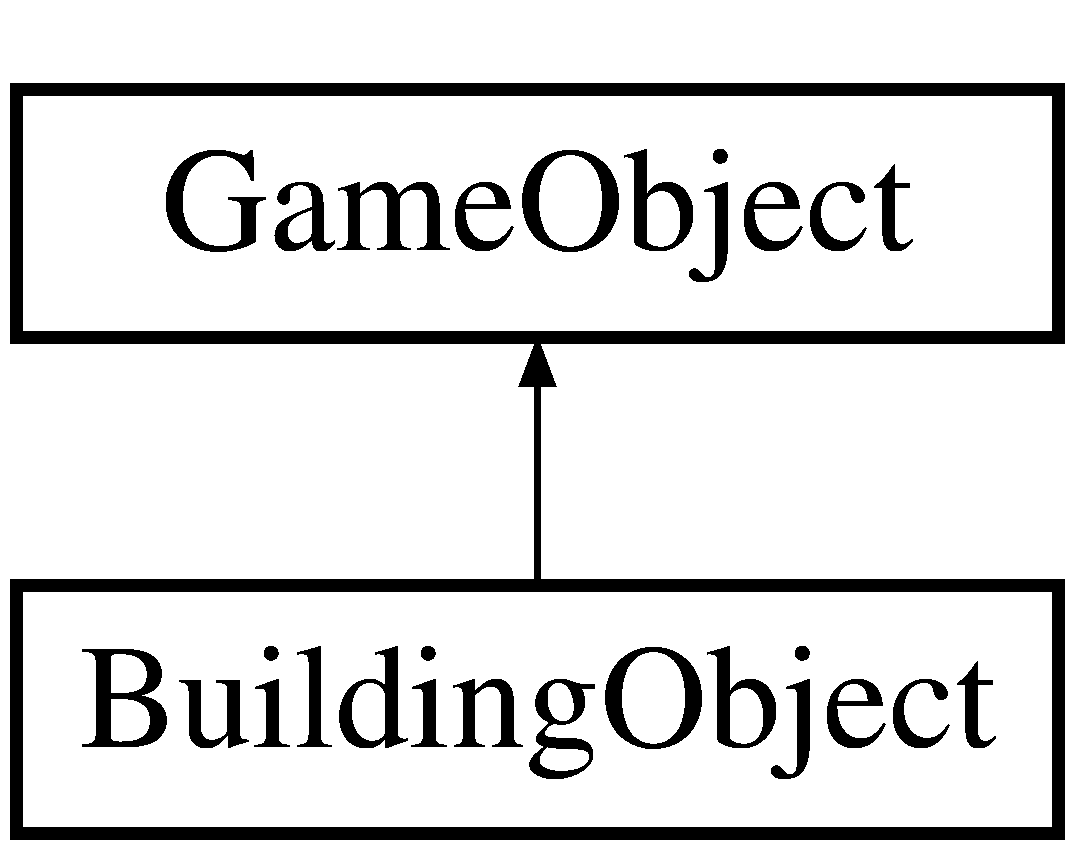
\includegraphics[height=2.000000cm]{class_building_object}
\end{center}
\end{figure}
\subsection*{Public Member Functions}
\begin{DoxyCompactItemize}
\item 
\mbox{\hyperlink{class_building_object_aab54197a4f72381251c422e530b5282f}{Building\+Object}} ()
\item 
\mbox{\hyperlink{class_building_object_a0a6779902609501186267d00d363bcde}{$\sim$\+Building\+Object}} ()
\item 
void \mbox{\hyperlink{class_building_object_a77221935bdcf6ef2cad7cd80fb877da8}{m\+\_\+\+Setup\+Building\+Object}} (sf\+::\+Vector2f dimentions, sf\+::\+Vector2f position, std\+::string building\+Type, \mbox{\hyperlink{class_cells}{Cells}} $\ast$new\+Cell, float wood\+Required)
\item 
void \mbox{\hyperlink{class_building_object_a74cbc1ffd32e6c4db6c645df2657e740}{m\+\_\+\+Assign\+Texture}} (sf\+::\+Texture $\ast$new\+Texture)
\item 
void \mbox{\hyperlink{class_building_object_a35fc31e0f1c9a1323b7dfedc527fccff}{m\+\_\+\+Update}} () override
\item 
void \mbox{\hyperlink{class_building_object_a7e343d32ad1f6aaed5ed484b2aabe700}{m\+\_\+\+Draw\+Game\+Object}} (sf\+::\+Render\+Window \&window) override
\item 
void \mbox{\hyperlink{class_building_object_a05e1b08fb5edd953b00e6deade8bad9d}{m\+\_\+\+Draw\+Filter}} (sf\+::\+Vector2f top\+Left, sf\+::\+Vector2f bottom\+Right) override
\item 
void \mbox{\hyperlink{class_building_object_a54130a69a81268544ca715275f52bfb7}{m\+\_\+\+Draw\+Filter}} (sf\+::\+Vector2f top\+Left, sf\+::\+Vector2f bottom\+Right, int current\+Layer)
\item 
void \mbox{\hyperlink{class_building_object_aa6239662e4277d8e1933f9c8fd487511}{m\+\_\+\+Set\+Object\+Pos}} (float x, float y) override
\item 
\mbox{\hyperlink{class_cells}{Cells}} $\ast$ \mbox{\hyperlink{class_building_object_aba3f08ddf833026289c2c0d36d0c40e3}{m\+\_\+\+Get\+Current\+Cell}} ()
\item 
bool \mbox{\hyperlink{class_building_object_a1d21e6caaa8853c9e60be5d80a5a42c1}{m\+\_\+\+Check\+Building\+Bounds}} (float x, float y)
\item 
void \mbox{\hyperlink{class_building_object_a3fd4003a55d98f537edfb002fc3726c1}{m\+\_\+\+Work\+Building}} (float work\+Speed)
\item 
void \mbox{\hyperlink{class_building_object_ade01ec444234c24eedc0286b5a7c85eb}{m\+\_\+\+Add\+Wood\+To\+Building}} (float wood\+To\+Add)
\item 
float \mbox{\hyperlink{class_building_object_a4cababbd690030d994111fbe8c7603b1}{m\+\_\+\+Get\+Wood\+Needed}} ()
\item 
bool \mbox{\hyperlink{class_building_object_aee720b050f8fed6e7f8cf773df7b0a3d}{m\+\_\+\+Need\+Wood}} ()
\item 
std\+::string \mbox{\hyperlink{class_building_object_af79abc387ac3519eb23bcea55a56a5b0}{m\+\_\+\+Get\+Building\+Type}} ()
\end{DoxyCompactItemize}
\subsection*{Public Attributes}
\begin{DoxyCompactItemize}
\item 
bool \mbox{\hyperlink{class_building_object_a2dd2d1f12b504e16b3bce3e8825badb7}{m\+\_\+b\+Finished\+Building}} = false
\end{DoxyCompactItemize}
\subsection*{Additional Inherited Members}


\subsection{Constructor \& Destructor Documentation}
\mbox{\Hypertarget{class_building_object_aab54197a4f72381251c422e530b5282f}\label{class_building_object_aab54197a4f72381251c422e530b5282f}} 
\index{Building\+Object@{Building\+Object}!Building\+Object@{Building\+Object}}
\index{Building\+Object@{Building\+Object}!Building\+Object@{Building\+Object}}
\subsubsection{\texorpdfstring{Building\+Object()}{BuildingObject()}}
{\footnotesize\ttfamily Building\+Object\+::\+Building\+Object (\begin{DoxyParamCaption}{ }\end{DoxyParamCaption})}

\mbox{\Hypertarget{class_building_object_a0a6779902609501186267d00d363bcde}\label{class_building_object_a0a6779902609501186267d00d363bcde}} 
\index{Building\+Object@{Building\+Object}!````~Building\+Object@{$\sim$\+Building\+Object}}
\index{````~Building\+Object@{$\sim$\+Building\+Object}!Building\+Object@{Building\+Object}}
\subsubsection{\texorpdfstring{$\sim$\+Building\+Object()}{~BuildingObject()}}
{\footnotesize\ttfamily Building\+Object\+::$\sim$\+Building\+Object (\begin{DoxyParamCaption}{ }\end{DoxyParamCaption})}



\subsection{Member Function Documentation}
\mbox{\Hypertarget{class_building_object_ade01ec444234c24eedc0286b5a7c85eb}\label{class_building_object_ade01ec444234c24eedc0286b5a7c85eb}} 
\index{Building\+Object@{Building\+Object}!m\+\_\+\+Add\+Wood\+To\+Building@{m\+\_\+\+Add\+Wood\+To\+Building}}
\index{m\+\_\+\+Add\+Wood\+To\+Building@{m\+\_\+\+Add\+Wood\+To\+Building}!Building\+Object@{Building\+Object}}
\subsubsection{\texorpdfstring{m\+\_\+\+Add\+Wood\+To\+Building()}{m\_AddWoodToBuilding()}}
{\footnotesize\ttfamily void Building\+Object\+::m\+\_\+\+Add\+Wood\+To\+Building (\begin{DoxyParamCaption}\item[{float}]{wood\+To\+Add }\end{DoxyParamCaption})}

\mbox{\Hypertarget{class_building_object_a74cbc1ffd32e6c4db6c645df2657e740}\label{class_building_object_a74cbc1ffd32e6c4db6c645df2657e740}} 
\index{Building\+Object@{Building\+Object}!m\+\_\+\+Assign\+Texture@{m\+\_\+\+Assign\+Texture}}
\index{m\+\_\+\+Assign\+Texture@{m\+\_\+\+Assign\+Texture}!Building\+Object@{Building\+Object}}
\subsubsection{\texorpdfstring{m\+\_\+\+Assign\+Texture()}{m\_AssignTexture()}}
{\footnotesize\ttfamily void Building\+Object\+::m\+\_\+\+Assign\+Texture (\begin{DoxyParamCaption}\item[{sf\+::\+Texture $\ast$}]{new\+Texture }\end{DoxyParamCaption})}

\mbox{\Hypertarget{class_building_object_a1d21e6caaa8853c9e60be5d80a5a42c1}\label{class_building_object_a1d21e6caaa8853c9e60be5d80a5a42c1}} 
\index{Building\+Object@{Building\+Object}!m\+\_\+\+Check\+Building\+Bounds@{m\+\_\+\+Check\+Building\+Bounds}}
\index{m\+\_\+\+Check\+Building\+Bounds@{m\+\_\+\+Check\+Building\+Bounds}!Building\+Object@{Building\+Object}}
\subsubsection{\texorpdfstring{m\+\_\+\+Check\+Building\+Bounds()}{m\_CheckBuildingBounds()}}
{\footnotesize\ttfamily bool Building\+Object\+::m\+\_\+\+Check\+Building\+Bounds (\begin{DoxyParamCaption}\item[{float}]{x,  }\item[{float}]{y }\end{DoxyParamCaption})}

\mbox{\Hypertarget{class_building_object_a05e1b08fb5edd953b00e6deade8bad9d}\label{class_building_object_a05e1b08fb5edd953b00e6deade8bad9d}} 
\index{Building\+Object@{Building\+Object}!m\+\_\+\+Draw\+Filter@{m\+\_\+\+Draw\+Filter}}
\index{m\+\_\+\+Draw\+Filter@{m\+\_\+\+Draw\+Filter}!Building\+Object@{Building\+Object}}
\subsubsection{\texorpdfstring{m\+\_\+\+Draw\+Filter()}{m\_DrawFilter()}\hspace{0.1cm}{\footnotesize\ttfamily [1/2]}}
{\footnotesize\ttfamily void Building\+Object\+::m\+\_\+\+Draw\+Filter (\begin{DoxyParamCaption}\item[{sf\+::\+Vector2f}]{top\+Left,  }\item[{sf\+::\+Vector2f}]{bottom\+Right }\end{DoxyParamCaption})\hspace{0.3cm}{\ttfamily [override]}, {\ttfamily [virtual]}}



Implements \mbox{\hyperlink{class_game_object_af1a0662ca445d878b163c4648f90259c}{Game\+Object}}.

\mbox{\Hypertarget{class_building_object_a54130a69a81268544ca715275f52bfb7}\label{class_building_object_a54130a69a81268544ca715275f52bfb7}} 
\index{Building\+Object@{Building\+Object}!m\+\_\+\+Draw\+Filter@{m\+\_\+\+Draw\+Filter}}
\index{m\+\_\+\+Draw\+Filter@{m\+\_\+\+Draw\+Filter}!Building\+Object@{Building\+Object}}
\subsubsection{\texorpdfstring{m\+\_\+\+Draw\+Filter()}{m\_DrawFilter()}\hspace{0.1cm}{\footnotesize\ttfamily [2/2]}}
{\footnotesize\ttfamily void Building\+Object\+::m\+\_\+\+Draw\+Filter (\begin{DoxyParamCaption}\item[{sf\+::\+Vector2f}]{top\+Left,  }\item[{sf\+::\+Vector2f}]{bottom\+Right,  }\item[{int}]{current\+Layer }\end{DoxyParamCaption})}

\mbox{\Hypertarget{class_building_object_a7e343d32ad1f6aaed5ed484b2aabe700}\label{class_building_object_a7e343d32ad1f6aaed5ed484b2aabe700}} 
\index{Building\+Object@{Building\+Object}!m\+\_\+\+Draw\+Game\+Object@{m\+\_\+\+Draw\+Game\+Object}}
\index{m\+\_\+\+Draw\+Game\+Object@{m\+\_\+\+Draw\+Game\+Object}!Building\+Object@{Building\+Object}}
\subsubsection{\texorpdfstring{m\+\_\+\+Draw\+Game\+Object()}{m\_DrawGameObject()}}
{\footnotesize\ttfamily void Building\+Object\+::m\+\_\+\+Draw\+Game\+Object (\begin{DoxyParamCaption}\item[{sf\+::\+Render\+Window \&}]{window }\end{DoxyParamCaption})\hspace{0.3cm}{\ttfamily [override]}, {\ttfamily [virtual]}}



Implements \mbox{\hyperlink{class_game_object_a184ac59fd5167c55a54b50894e5b6721}{Game\+Object}}.

\mbox{\Hypertarget{class_building_object_af79abc387ac3519eb23bcea55a56a5b0}\label{class_building_object_af79abc387ac3519eb23bcea55a56a5b0}} 
\index{Building\+Object@{Building\+Object}!m\+\_\+\+Get\+Building\+Type@{m\+\_\+\+Get\+Building\+Type}}
\index{m\+\_\+\+Get\+Building\+Type@{m\+\_\+\+Get\+Building\+Type}!Building\+Object@{Building\+Object}}
\subsubsection{\texorpdfstring{m\+\_\+\+Get\+Building\+Type()}{m\_GetBuildingType()}}
{\footnotesize\ttfamily std\+::string Building\+Object\+::m\+\_\+\+Get\+Building\+Type (\begin{DoxyParamCaption}{ }\end{DoxyParamCaption})}

\mbox{\Hypertarget{class_building_object_aba3f08ddf833026289c2c0d36d0c40e3}\label{class_building_object_aba3f08ddf833026289c2c0d36d0c40e3}} 
\index{Building\+Object@{Building\+Object}!m\+\_\+\+Get\+Current\+Cell@{m\+\_\+\+Get\+Current\+Cell}}
\index{m\+\_\+\+Get\+Current\+Cell@{m\+\_\+\+Get\+Current\+Cell}!Building\+Object@{Building\+Object}}
\subsubsection{\texorpdfstring{m\+\_\+\+Get\+Current\+Cell()}{m\_GetCurrentCell()}}
{\footnotesize\ttfamily \mbox{\hyperlink{class_cells}{Cells}}$\ast$ Building\+Object\+::m\+\_\+\+Get\+Current\+Cell (\begin{DoxyParamCaption}{ }\end{DoxyParamCaption})}

\mbox{\Hypertarget{class_building_object_a4cababbd690030d994111fbe8c7603b1}\label{class_building_object_a4cababbd690030d994111fbe8c7603b1}} 
\index{Building\+Object@{Building\+Object}!m\+\_\+\+Get\+Wood\+Needed@{m\+\_\+\+Get\+Wood\+Needed}}
\index{m\+\_\+\+Get\+Wood\+Needed@{m\+\_\+\+Get\+Wood\+Needed}!Building\+Object@{Building\+Object}}
\subsubsection{\texorpdfstring{m\+\_\+\+Get\+Wood\+Needed()}{m\_GetWoodNeeded()}}
{\footnotesize\ttfamily float Building\+Object\+::m\+\_\+\+Get\+Wood\+Needed (\begin{DoxyParamCaption}{ }\end{DoxyParamCaption})}

\mbox{\Hypertarget{class_building_object_aee720b050f8fed6e7f8cf773df7b0a3d}\label{class_building_object_aee720b050f8fed6e7f8cf773df7b0a3d}} 
\index{Building\+Object@{Building\+Object}!m\+\_\+\+Need\+Wood@{m\+\_\+\+Need\+Wood}}
\index{m\+\_\+\+Need\+Wood@{m\+\_\+\+Need\+Wood}!Building\+Object@{Building\+Object}}
\subsubsection{\texorpdfstring{m\+\_\+\+Need\+Wood()}{m\_NeedWood()}}
{\footnotesize\ttfamily bool Building\+Object\+::m\+\_\+\+Need\+Wood (\begin{DoxyParamCaption}{ }\end{DoxyParamCaption})}

\mbox{\Hypertarget{class_building_object_aa6239662e4277d8e1933f9c8fd487511}\label{class_building_object_aa6239662e4277d8e1933f9c8fd487511}} 
\index{Building\+Object@{Building\+Object}!m\+\_\+\+Set\+Object\+Pos@{m\+\_\+\+Set\+Object\+Pos}}
\index{m\+\_\+\+Set\+Object\+Pos@{m\+\_\+\+Set\+Object\+Pos}!Building\+Object@{Building\+Object}}
\subsubsection{\texorpdfstring{m\+\_\+\+Set\+Object\+Pos()}{m\_SetObjectPos()}}
{\footnotesize\ttfamily void Building\+Object\+::m\+\_\+\+Set\+Object\+Pos (\begin{DoxyParamCaption}\item[{float}]{x,  }\item[{float}]{y }\end{DoxyParamCaption})\hspace{0.3cm}{\ttfamily [override]}, {\ttfamily [virtual]}}



Implements \mbox{\hyperlink{class_game_object_ad1f8ea8eb3673b1af8215bf92cdc0df8}{Game\+Object}}.

\mbox{\Hypertarget{class_building_object_a77221935bdcf6ef2cad7cd80fb877da8}\label{class_building_object_a77221935bdcf6ef2cad7cd80fb877da8}} 
\index{Building\+Object@{Building\+Object}!m\+\_\+\+Setup\+Building\+Object@{m\+\_\+\+Setup\+Building\+Object}}
\index{m\+\_\+\+Setup\+Building\+Object@{m\+\_\+\+Setup\+Building\+Object}!Building\+Object@{Building\+Object}}
\subsubsection{\texorpdfstring{m\+\_\+\+Setup\+Building\+Object()}{m\_SetupBuildingObject()}}
{\footnotesize\ttfamily void Building\+Object\+::m\+\_\+\+Setup\+Building\+Object (\begin{DoxyParamCaption}\item[{sf\+::\+Vector2f}]{dimentions,  }\item[{sf\+::\+Vector2f}]{position,  }\item[{std\+::string}]{building\+Type,  }\item[{\mbox{\hyperlink{class_cells}{Cells}} $\ast$}]{new\+Cell,  }\item[{float}]{wood\+Required }\end{DoxyParamCaption})}

\mbox{\Hypertarget{class_building_object_a35fc31e0f1c9a1323b7dfedc527fccff}\label{class_building_object_a35fc31e0f1c9a1323b7dfedc527fccff}} 
\index{Building\+Object@{Building\+Object}!m\+\_\+\+Update@{m\+\_\+\+Update}}
\index{m\+\_\+\+Update@{m\+\_\+\+Update}!Building\+Object@{Building\+Object}}
\subsubsection{\texorpdfstring{m\+\_\+\+Update()}{m\_Update()}}
{\footnotesize\ttfamily void Building\+Object\+::m\+\_\+\+Update (\begin{DoxyParamCaption}{ }\end{DoxyParamCaption})\hspace{0.3cm}{\ttfamily [override]}, {\ttfamily [virtual]}}



Implements \mbox{\hyperlink{class_game_object_a3af5a7b470e09f13a1422439fc6a9ba8}{Game\+Object}}.

\mbox{\Hypertarget{class_building_object_a3fd4003a55d98f537edfb002fc3726c1}\label{class_building_object_a3fd4003a55d98f537edfb002fc3726c1}} 
\index{Building\+Object@{Building\+Object}!m\+\_\+\+Work\+Building@{m\+\_\+\+Work\+Building}}
\index{m\+\_\+\+Work\+Building@{m\+\_\+\+Work\+Building}!Building\+Object@{Building\+Object}}
\subsubsection{\texorpdfstring{m\+\_\+\+Work\+Building()}{m\_WorkBuilding()}}
{\footnotesize\ttfamily void Building\+Object\+::m\+\_\+\+Work\+Building (\begin{DoxyParamCaption}\item[{float}]{work\+Speed }\end{DoxyParamCaption})}



\subsection{Member Data Documentation}
\mbox{\Hypertarget{class_building_object_a2dd2d1f12b504e16b3bce3e8825badb7}\label{class_building_object_a2dd2d1f12b504e16b3bce3e8825badb7}} 
\index{Building\+Object@{Building\+Object}!m\+\_\+b\+Finished\+Building@{m\+\_\+b\+Finished\+Building}}
\index{m\+\_\+b\+Finished\+Building@{m\+\_\+b\+Finished\+Building}!Building\+Object@{Building\+Object}}
\subsubsection{\texorpdfstring{m\+\_\+b\+Finished\+Building}{m\_bFinishedBuilding}}
{\footnotesize\ttfamily bool Building\+Object\+::m\+\_\+b\+Finished\+Building = false}



The documentation for this class was generated from the following file\+:\begin{DoxyCompactItemize}
\item 
inc/\mbox{\hyperlink{_building_object_8h}{Building\+Object.\+h}}\end{DoxyCompactItemize}

\hypertarget{class_cells}{}\section{Cells Class Reference}
\label{class_cells}\index{Cells@{Cells}}


{\ttfamily \#include $<$Cells.\+h$>$}

Inheritance diagram for Cells\+:\begin{figure}[H]
\begin{center}
\leavevmode
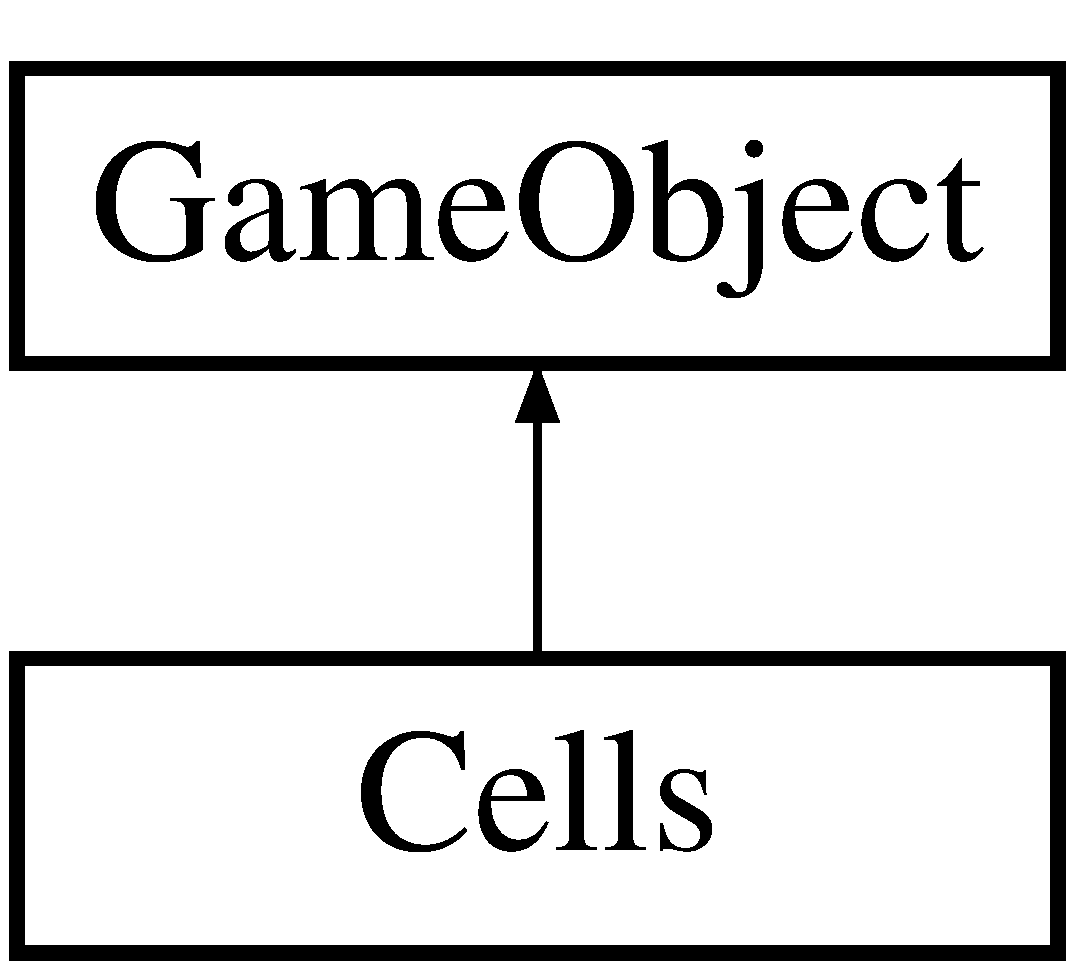
\includegraphics[height=2.000000cm]{class_cells}
\end{center}
\end{figure}
\subsection*{Public Member Functions}
\begin{DoxyCompactItemize}
\item 
\mbox{\hyperlink{class_cells_a092d62bc15648a54755a413dbf9a2db0}{Cells}} ()
\item 
\mbox{\hyperlink{class_cells_aab121634db81b439226a33fd099fb3c1}{$\sim$\+Cells}} ()
\item 
void \mbox{\hyperlink{class_cells_a5f009c592371d6bad0e49b2ff2bfd811}{m\+\_\+\+Create\+Cell\+Body}} (sf\+::\+Vector2f dimentions, sf\+::\+Vector2f possition)
\item 
void \mbox{\hyperlink{class_cells_a6405637a987f8af6210518d21b284c5d}{m\+\_\+\+Create\+Cell\+Body}} (sf\+::\+Vector2f dimentions, sf\+::\+Vector2f possition, int r, int g, int b)
\item 
void \mbox{\hyperlink{class_cells_a943b866ae140765aaa6d8113ad68065c}{m\+\_\+\+Assign\+Texture}} (sf\+::\+Texture new\+Texture)
\item 
bool \mbox{\hyperlink{class_cells_a49ad6477b62bb29973f3e248909e216b}{m\+\_\+\+Check\+Cell\+Bounds}} (float x, float y)
\item 
void \mbox{\hyperlink{class_cells_abf00b8c57ba89e13c2ee86f22051e56f}{m\+\_\+\+Set\+Cell\+Centre}} ()
\item 
void \mbox{\hyperlink{class_cells_a5d900205d8d5fc3d3b41b664d51994c4}{m\+\_\+\+Set\+Object\+Pos}} (float x, float y) override
\item 
sf\+::\+Vector2f \mbox{\hyperlink{class_cells_ae61d97e90ef66528c67be257531c4359}{m\+\_\+\+Get\+Cell\+Centre}} ()
\item 
void \mbox{\hyperlink{class_cells_a54a485e9bed0760a0a7464311b59a700}{m\+\_\+\+Set\+Cell\+Colour}} (int r, int g, int b)
\item 
void \mbox{\hyperlink{class_cells_a4f59f13bfeec4f70dbd2133e86b747eb}{m\+\_\+\+Assign\+Colours}} ()
\item 
void \mbox{\hyperlink{class_cells_ace2656aa881803e17d7d53c9031e6ee4}{m\+\_\+\+Set\+Grid\+Pos}} (int x, int y)
\item 
\mbox{\hyperlink{structgrid_pos}{grid\+Pos}} \mbox{\hyperlink{class_cells_a81750cfd622629b65d615cec1d4edb48}{m\+\_\+\+Get\+Grid\+Pos}} ()
\item 
void \mbox{\hyperlink{class_cells_a4978491aa8ad58dd1c1f2ad0431d78b6}{m\+\_\+\+Set\+Layer}} (int layer)
\item 
int \mbox{\hyperlink{class_cells_ad45ab05eb579aa75a0c67c03eaefc0c0}{m\+\_\+\+Get\+Layer}} ()
\item 
void \mbox{\hyperlink{class_cells_a2d2d122fb7611a3f2c06f0e44b32dcdc}{m\+\_\+\+Assign\+Neighbour}} (\mbox{\hyperlink{class_cells}{Cells}} \&neighbour)
\item 
std\+::vector$<$ \mbox{\hyperlink{class_cells}{Cells}} $\ast$ $>$ \& \mbox{\hyperlink{class_cells_ab1b7667ae7e690e9e763d1dd02a5a46e}{m\+\_\+\+Get\+Neighbours}} ()
\item 
int \mbox{\hyperlink{class_cells_a230bc14139877d4b703d087784a0c5bc}{m\+\_\+\+Get\+Cell\+Id}} ()
\item 
void \mbox{\hyperlink{class_cells_a72a566e099b35379c90ad4e90bbcd793}{m\+\_\+\+Assign\+Cell\+Id}} (int id)
\item 
\mbox{\hyperlink{_cells_8h_adc5e4636eae42cdad2a070c6adbd9daf}{tile\+Set}} \mbox{\hyperlink{class_cells_a1ee8670d06fa37bbdbdb30796c0eeee0}{m\+\_\+\+Get\+Tile}} ()
\item 
void \mbox{\hyperlink{class_cells_a2b96194a69da35f886dc0bb542a4b3b8}{m\+\_\+\+Assign\+Tile}} (\mbox{\hyperlink{_cells_8h_adc5e4636eae42cdad2a070c6adbd9daf}{tile\+Set}} which\+Tile)
\item 
std\+::string \mbox{\hyperlink{class_cells_ae64b76c5e33a081910b1c93631f8dd4e}{m\+\_\+\+Get\+Tile\+Name}} ()
\item 
float \mbox{\hyperlink{class_cells_a8697fccb916059fd456256d038d8f1c2}{m\+\_\+\+Get\+Cell\+Width}} ()
\item 
float \mbox{\hyperlink{class_cells_ac5885d8ebc2418182b48d19b9e7fde08}{m\+\_\+\+Get\+Cell\+Height}} ()
\item 
void \mbox{\hyperlink{class_cells_a524d410412de7030016b99a4d8b0c1cc}{m\+\_\+\+Update}} () override
\item 
void \mbox{\hyperlink{class_cells_a09ab1aeac5c986cc28f52754fafd8c66}{m\+\_\+\+Draw\+Game\+Object}} (sf\+::\+Render\+Window \&window) override
\item 
void \mbox{\hyperlink{class_cells_a9c7eea82ba5ab8a840bbdcc0be25200f}{m\+\_\+\+Draw\+Filter}} (sf\+::\+Vector2f top\+Left, sf\+::\+Vector2f bottom\+Right) override
\end{DoxyCompactItemize}
\subsection*{Public Attributes}
\begin{DoxyCompactItemize}
\item 
\mbox{\hyperlink{class_cells}{Cells}} $\ast$ \mbox{\hyperlink{class_cells_ae71aff17afdd01c99293906893c67354}{m\+\_\+\+Parent\+Cell}} = nullptr
\item 
int \mbox{\hyperlink{class_cells_abe9c29d1ede13bf4fe3980ab837e81ce}{m\+\_\+i\+G\+Score}} = 0
\item 
int \mbox{\hyperlink{class_cells_a00f6a71c14e40130259bbdeb15394f67}{m\+\_\+i\+H\+Score}} = 0
\item 
int \mbox{\hyperlink{class_cells_a4c0eadc267ff60babcabe97347d9e452}{m\+\_\+i\+F\+Score}} = 0
\item 
bool \mbox{\hyperlink{class_cells_a0bc31e333f70a4d5aefd1fa5e14fa0fb}{m\+\_\+b\+Obstruction}} = false
\end{DoxyCompactItemize}
\subsection*{Additional Inherited Members}


\subsection{Detailed Description}
up form a grid, each cell will represent a single point within a grid. 

\subsection{Constructor \& Destructor Documentation}
\mbox{\Hypertarget{class_cells_a092d62bc15648a54755a413dbf9a2db0}\label{class_cells_a092d62bc15648a54755a413dbf9a2db0}} 
\index{Cells@{Cells}!Cells@{Cells}}
\index{Cells@{Cells}!Cells@{Cells}}
\subsubsection{\texorpdfstring{Cells()}{Cells()}}
{\footnotesize\ttfamily Cells\+::\+Cells (\begin{DoxyParamCaption}{ }\end{DoxyParamCaption})}

\mbox{\Hypertarget{class_cells_aab121634db81b439226a33fd099fb3c1}\label{class_cells_aab121634db81b439226a33fd099fb3c1}} 
\index{Cells@{Cells}!````~Cells@{$\sim$\+Cells}}
\index{````~Cells@{$\sim$\+Cells}!Cells@{Cells}}
\subsubsection{\texorpdfstring{$\sim$\+Cells()}{~Cells()}}
{\footnotesize\ttfamily Cells\+::$\sim$\+Cells (\begin{DoxyParamCaption}{ }\end{DoxyParamCaption})}



\subsection{Member Function Documentation}
\mbox{\Hypertarget{class_cells_a72a566e099b35379c90ad4e90bbcd793}\label{class_cells_a72a566e099b35379c90ad4e90bbcd793}} 
\index{Cells@{Cells}!m\+\_\+\+Assign\+Cell\+Id@{m\+\_\+\+Assign\+Cell\+Id}}
\index{m\+\_\+\+Assign\+Cell\+Id@{m\+\_\+\+Assign\+Cell\+Id}!Cells@{Cells}}
\subsubsection{\texorpdfstring{m\+\_\+\+Assign\+Cell\+Id()}{m\_AssignCellId()}}
{\footnotesize\ttfamily void Cells\+::m\+\_\+\+Assign\+Cell\+Id (\begin{DoxyParamCaption}\item[{int}]{id }\end{DoxyParamCaption})}

\mbox{\Hypertarget{class_cells_a4f59f13bfeec4f70dbd2133e86b747eb}\label{class_cells_a4f59f13bfeec4f70dbd2133e86b747eb}} 
\index{Cells@{Cells}!m\+\_\+\+Assign\+Colours@{m\+\_\+\+Assign\+Colours}}
\index{m\+\_\+\+Assign\+Colours@{m\+\_\+\+Assign\+Colours}!Cells@{Cells}}
\subsubsection{\texorpdfstring{m\+\_\+\+Assign\+Colours()}{m\_AssignColours()}}
{\footnotesize\ttfamily void Cells\+::m\+\_\+\+Assign\+Colours (\begin{DoxyParamCaption}{ }\end{DoxyParamCaption})}

\mbox{\Hypertarget{class_cells_a2d2d122fb7611a3f2c06f0e44b32dcdc}\label{class_cells_a2d2d122fb7611a3f2c06f0e44b32dcdc}} 
\index{Cells@{Cells}!m\+\_\+\+Assign\+Neighbour@{m\+\_\+\+Assign\+Neighbour}}
\index{m\+\_\+\+Assign\+Neighbour@{m\+\_\+\+Assign\+Neighbour}!Cells@{Cells}}
\subsubsection{\texorpdfstring{m\+\_\+\+Assign\+Neighbour()}{m\_AssignNeighbour()}}
{\footnotesize\ttfamily void Cells\+::m\+\_\+\+Assign\+Neighbour (\begin{DoxyParamCaption}\item[{\mbox{\hyperlink{class_cells}{Cells}} \&}]{neighbour }\end{DoxyParamCaption})}

\mbox{\Hypertarget{class_cells_a943b866ae140765aaa6d8113ad68065c}\label{class_cells_a943b866ae140765aaa6d8113ad68065c}} 
\index{Cells@{Cells}!m\+\_\+\+Assign\+Texture@{m\+\_\+\+Assign\+Texture}}
\index{m\+\_\+\+Assign\+Texture@{m\+\_\+\+Assign\+Texture}!Cells@{Cells}}
\subsubsection{\texorpdfstring{m\+\_\+\+Assign\+Texture()}{m\_AssignTexture()}}
{\footnotesize\ttfamily void Cells\+::m\+\_\+\+Assign\+Texture (\begin{DoxyParamCaption}\item[{sf\+::\+Texture}]{new\+Texture }\end{DoxyParamCaption})}

\mbox{\Hypertarget{class_cells_a2b96194a69da35f886dc0bb542a4b3b8}\label{class_cells_a2b96194a69da35f886dc0bb542a4b3b8}} 
\index{Cells@{Cells}!m\+\_\+\+Assign\+Tile@{m\+\_\+\+Assign\+Tile}}
\index{m\+\_\+\+Assign\+Tile@{m\+\_\+\+Assign\+Tile}!Cells@{Cells}}
\subsubsection{\texorpdfstring{m\+\_\+\+Assign\+Tile()}{m\_AssignTile()}}
{\footnotesize\ttfamily void Cells\+::m\+\_\+\+Assign\+Tile (\begin{DoxyParamCaption}\item[{\mbox{\hyperlink{_cells_8h_adc5e4636eae42cdad2a070c6adbd9daf}{tile\+Set}}}]{which\+Tile }\end{DoxyParamCaption})}

\mbox{\Hypertarget{class_cells_a49ad6477b62bb29973f3e248909e216b}\label{class_cells_a49ad6477b62bb29973f3e248909e216b}} 
\index{Cells@{Cells}!m\+\_\+\+Check\+Cell\+Bounds@{m\+\_\+\+Check\+Cell\+Bounds}}
\index{m\+\_\+\+Check\+Cell\+Bounds@{m\+\_\+\+Check\+Cell\+Bounds}!Cells@{Cells}}
\subsubsection{\texorpdfstring{m\+\_\+\+Check\+Cell\+Bounds()}{m\_CheckCellBounds()}}
{\footnotesize\ttfamily bool Cells\+::m\+\_\+\+Check\+Cell\+Bounds (\begin{DoxyParamCaption}\item[{float}]{x,  }\item[{float}]{y }\end{DoxyParamCaption})}

\mbox{\Hypertarget{class_cells_a5f009c592371d6bad0e49b2ff2bfd811}\label{class_cells_a5f009c592371d6bad0e49b2ff2bfd811}} 
\index{Cells@{Cells}!m\+\_\+\+Create\+Cell\+Body@{m\+\_\+\+Create\+Cell\+Body}}
\index{m\+\_\+\+Create\+Cell\+Body@{m\+\_\+\+Create\+Cell\+Body}!Cells@{Cells}}
\subsubsection{\texorpdfstring{m\+\_\+\+Create\+Cell\+Body()}{m\_CreateCellBody()}\hspace{0.1cm}{\footnotesize\ttfamily [1/2]}}
{\footnotesize\ttfamily void Cells\+::m\+\_\+\+Create\+Cell\+Body (\begin{DoxyParamCaption}\item[{sf\+::\+Vector2f}]{dimentions,  }\item[{sf\+::\+Vector2f}]{possition }\end{DoxyParamCaption})}

\mbox{\Hypertarget{class_cells_a6405637a987f8af6210518d21b284c5d}\label{class_cells_a6405637a987f8af6210518d21b284c5d}} 
\index{Cells@{Cells}!m\+\_\+\+Create\+Cell\+Body@{m\+\_\+\+Create\+Cell\+Body}}
\index{m\+\_\+\+Create\+Cell\+Body@{m\+\_\+\+Create\+Cell\+Body}!Cells@{Cells}}
\subsubsection{\texorpdfstring{m\+\_\+\+Create\+Cell\+Body()}{m\_CreateCellBody()}\hspace{0.1cm}{\footnotesize\ttfamily [2/2]}}
{\footnotesize\ttfamily void Cells\+::m\+\_\+\+Create\+Cell\+Body (\begin{DoxyParamCaption}\item[{sf\+::\+Vector2f}]{dimentions,  }\item[{sf\+::\+Vector2f}]{possition,  }\item[{int}]{r,  }\item[{int}]{g,  }\item[{int}]{b }\end{DoxyParamCaption})}

\mbox{\Hypertarget{class_cells_a9c7eea82ba5ab8a840bbdcc0be25200f}\label{class_cells_a9c7eea82ba5ab8a840bbdcc0be25200f}} 
\index{Cells@{Cells}!m\+\_\+\+Draw\+Filter@{m\+\_\+\+Draw\+Filter}}
\index{m\+\_\+\+Draw\+Filter@{m\+\_\+\+Draw\+Filter}!Cells@{Cells}}
\subsubsection{\texorpdfstring{m\+\_\+\+Draw\+Filter()}{m\_DrawFilter()}}
{\footnotesize\ttfamily void Cells\+::m\+\_\+\+Draw\+Filter (\begin{DoxyParamCaption}\item[{sf\+::\+Vector2f}]{top\+Left,  }\item[{sf\+::\+Vector2f}]{bottom\+Right }\end{DoxyParamCaption})\hspace{0.3cm}{\ttfamily [override]}, {\ttfamily [virtual]}}



Implements \mbox{\hyperlink{class_game_object_af1a0662ca445d878b163c4648f90259c}{Game\+Object}}.

\mbox{\Hypertarget{class_cells_a09ab1aeac5c986cc28f52754fafd8c66}\label{class_cells_a09ab1aeac5c986cc28f52754fafd8c66}} 
\index{Cells@{Cells}!m\+\_\+\+Draw\+Game\+Object@{m\+\_\+\+Draw\+Game\+Object}}
\index{m\+\_\+\+Draw\+Game\+Object@{m\+\_\+\+Draw\+Game\+Object}!Cells@{Cells}}
\subsubsection{\texorpdfstring{m\+\_\+\+Draw\+Game\+Object()}{m\_DrawGameObject()}}
{\footnotesize\ttfamily void Cells\+::m\+\_\+\+Draw\+Game\+Object (\begin{DoxyParamCaption}\item[{sf\+::\+Render\+Window \&}]{window }\end{DoxyParamCaption})\hspace{0.3cm}{\ttfamily [override]}, {\ttfamily [virtual]}}



Implements \mbox{\hyperlink{class_game_object_a184ac59fd5167c55a54b50894e5b6721}{Game\+Object}}.

\mbox{\Hypertarget{class_cells_ae61d97e90ef66528c67be257531c4359}\label{class_cells_ae61d97e90ef66528c67be257531c4359}} 
\index{Cells@{Cells}!m\+\_\+\+Get\+Cell\+Centre@{m\+\_\+\+Get\+Cell\+Centre}}
\index{m\+\_\+\+Get\+Cell\+Centre@{m\+\_\+\+Get\+Cell\+Centre}!Cells@{Cells}}
\subsubsection{\texorpdfstring{m\+\_\+\+Get\+Cell\+Centre()}{m\_GetCellCentre()}}
{\footnotesize\ttfamily sf\+::\+Vector2f Cells\+::m\+\_\+\+Get\+Cell\+Centre (\begin{DoxyParamCaption}{ }\end{DoxyParamCaption})}

\mbox{\Hypertarget{class_cells_ac5885d8ebc2418182b48d19b9e7fde08}\label{class_cells_ac5885d8ebc2418182b48d19b9e7fde08}} 
\index{Cells@{Cells}!m\+\_\+\+Get\+Cell\+Height@{m\+\_\+\+Get\+Cell\+Height}}
\index{m\+\_\+\+Get\+Cell\+Height@{m\+\_\+\+Get\+Cell\+Height}!Cells@{Cells}}
\subsubsection{\texorpdfstring{m\+\_\+\+Get\+Cell\+Height()}{m\_GetCellHeight()}}
{\footnotesize\ttfamily float Cells\+::m\+\_\+\+Get\+Cell\+Height (\begin{DoxyParamCaption}{ }\end{DoxyParamCaption})}

\mbox{\Hypertarget{class_cells_a230bc14139877d4b703d087784a0c5bc}\label{class_cells_a230bc14139877d4b703d087784a0c5bc}} 
\index{Cells@{Cells}!m\+\_\+\+Get\+Cell\+Id@{m\+\_\+\+Get\+Cell\+Id}}
\index{m\+\_\+\+Get\+Cell\+Id@{m\+\_\+\+Get\+Cell\+Id}!Cells@{Cells}}
\subsubsection{\texorpdfstring{m\+\_\+\+Get\+Cell\+Id()}{m\_GetCellId()}}
{\footnotesize\ttfamily int Cells\+::m\+\_\+\+Get\+Cell\+Id (\begin{DoxyParamCaption}{ }\end{DoxyParamCaption})}

\mbox{\Hypertarget{class_cells_a8697fccb916059fd456256d038d8f1c2}\label{class_cells_a8697fccb916059fd456256d038d8f1c2}} 
\index{Cells@{Cells}!m\+\_\+\+Get\+Cell\+Width@{m\+\_\+\+Get\+Cell\+Width}}
\index{m\+\_\+\+Get\+Cell\+Width@{m\+\_\+\+Get\+Cell\+Width}!Cells@{Cells}}
\subsubsection{\texorpdfstring{m\+\_\+\+Get\+Cell\+Width()}{m\_GetCellWidth()}}
{\footnotesize\ttfamily float Cells\+::m\+\_\+\+Get\+Cell\+Width (\begin{DoxyParamCaption}{ }\end{DoxyParamCaption})}

\mbox{\Hypertarget{class_cells_a81750cfd622629b65d615cec1d4edb48}\label{class_cells_a81750cfd622629b65d615cec1d4edb48}} 
\index{Cells@{Cells}!m\+\_\+\+Get\+Grid\+Pos@{m\+\_\+\+Get\+Grid\+Pos}}
\index{m\+\_\+\+Get\+Grid\+Pos@{m\+\_\+\+Get\+Grid\+Pos}!Cells@{Cells}}
\subsubsection{\texorpdfstring{m\+\_\+\+Get\+Grid\+Pos()}{m\_GetGridPos()}}
{\footnotesize\ttfamily \mbox{\hyperlink{structgrid_pos}{grid\+Pos}} Cells\+::m\+\_\+\+Get\+Grid\+Pos (\begin{DoxyParamCaption}{ }\end{DoxyParamCaption})}

\mbox{\Hypertarget{class_cells_ad45ab05eb579aa75a0c67c03eaefc0c0}\label{class_cells_ad45ab05eb579aa75a0c67c03eaefc0c0}} 
\index{Cells@{Cells}!m\+\_\+\+Get\+Layer@{m\+\_\+\+Get\+Layer}}
\index{m\+\_\+\+Get\+Layer@{m\+\_\+\+Get\+Layer}!Cells@{Cells}}
\subsubsection{\texorpdfstring{m\+\_\+\+Get\+Layer()}{m\_GetLayer()}}
{\footnotesize\ttfamily int Cells\+::m\+\_\+\+Get\+Layer (\begin{DoxyParamCaption}{ }\end{DoxyParamCaption})}

\mbox{\Hypertarget{class_cells_ab1b7667ae7e690e9e763d1dd02a5a46e}\label{class_cells_ab1b7667ae7e690e9e763d1dd02a5a46e}} 
\index{Cells@{Cells}!m\+\_\+\+Get\+Neighbours@{m\+\_\+\+Get\+Neighbours}}
\index{m\+\_\+\+Get\+Neighbours@{m\+\_\+\+Get\+Neighbours}!Cells@{Cells}}
\subsubsection{\texorpdfstring{m\+\_\+\+Get\+Neighbours()}{m\_GetNeighbours()}}
{\footnotesize\ttfamily std\+::vector$<$\mbox{\hyperlink{class_cells}{Cells}}$\ast$$>$\& Cells\+::m\+\_\+\+Get\+Neighbours (\begin{DoxyParamCaption}{ }\end{DoxyParamCaption})}

\mbox{\Hypertarget{class_cells_a1ee8670d06fa37bbdbdb30796c0eeee0}\label{class_cells_a1ee8670d06fa37bbdbdb30796c0eeee0}} 
\index{Cells@{Cells}!m\+\_\+\+Get\+Tile@{m\+\_\+\+Get\+Tile}}
\index{m\+\_\+\+Get\+Tile@{m\+\_\+\+Get\+Tile}!Cells@{Cells}}
\subsubsection{\texorpdfstring{m\+\_\+\+Get\+Tile()}{m\_GetTile()}}
{\footnotesize\ttfamily \mbox{\hyperlink{_cells_8h_adc5e4636eae42cdad2a070c6adbd9daf}{tile\+Set}} Cells\+::m\+\_\+\+Get\+Tile (\begin{DoxyParamCaption}{ }\end{DoxyParamCaption})}

\mbox{\Hypertarget{class_cells_ae64b76c5e33a081910b1c93631f8dd4e}\label{class_cells_ae64b76c5e33a081910b1c93631f8dd4e}} 
\index{Cells@{Cells}!m\+\_\+\+Get\+Tile\+Name@{m\+\_\+\+Get\+Tile\+Name}}
\index{m\+\_\+\+Get\+Tile\+Name@{m\+\_\+\+Get\+Tile\+Name}!Cells@{Cells}}
\subsubsection{\texorpdfstring{m\+\_\+\+Get\+Tile\+Name()}{m\_GetTileName()}}
{\footnotesize\ttfamily std\+::string Cells\+::m\+\_\+\+Get\+Tile\+Name (\begin{DoxyParamCaption}{ }\end{DoxyParamCaption})}

\mbox{\Hypertarget{class_cells_abf00b8c57ba89e13c2ee86f22051e56f}\label{class_cells_abf00b8c57ba89e13c2ee86f22051e56f}} 
\index{Cells@{Cells}!m\+\_\+\+Set\+Cell\+Centre@{m\+\_\+\+Set\+Cell\+Centre}}
\index{m\+\_\+\+Set\+Cell\+Centre@{m\+\_\+\+Set\+Cell\+Centre}!Cells@{Cells}}
\subsubsection{\texorpdfstring{m\+\_\+\+Set\+Cell\+Centre()}{m\_SetCellCentre()}}
{\footnotesize\ttfamily void Cells\+::m\+\_\+\+Set\+Cell\+Centre (\begin{DoxyParamCaption}{ }\end{DoxyParamCaption})}

\mbox{\Hypertarget{class_cells_a54a485e9bed0760a0a7464311b59a700}\label{class_cells_a54a485e9bed0760a0a7464311b59a700}} 
\index{Cells@{Cells}!m\+\_\+\+Set\+Cell\+Colour@{m\+\_\+\+Set\+Cell\+Colour}}
\index{m\+\_\+\+Set\+Cell\+Colour@{m\+\_\+\+Set\+Cell\+Colour}!Cells@{Cells}}
\subsubsection{\texorpdfstring{m\+\_\+\+Set\+Cell\+Colour()}{m\_SetCellColour()}}
{\footnotesize\ttfamily void Cells\+::m\+\_\+\+Set\+Cell\+Colour (\begin{DoxyParamCaption}\item[{int}]{r,  }\item[{int}]{g,  }\item[{int}]{b }\end{DoxyParamCaption})}

\mbox{\Hypertarget{class_cells_ace2656aa881803e17d7d53c9031e6ee4}\label{class_cells_ace2656aa881803e17d7d53c9031e6ee4}} 
\index{Cells@{Cells}!m\+\_\+\+Set\+Grid\+Pos@{m\+\_\+\+Set\+Grid\+Pos}}
\index{m\+\_\+\+Set\+Grid\+Pos@{m\+\_\+\+Set\+Grid\+Pos}!Cells@{Cells}}
\subsubsection{\texorpdfstring{m\+\_\+\+Set\+Grid\+Pos()}{m\_SetGridPos()}}
{\footnotesize\ttfamily void Cells\+::m\+\_\+\+Set\+Grid\+Pos (\begin{DoxyParamCaption}\item[{int}]{x,  }\item[{int}]{y }\end{DoxyParamCaption})}

\mbox{\Hypertarget{class_cells_a4978491aa8ad58dd1c1f2ad0431d78b6}\label{class_cells_a4978491aa8ad58dd1c1f2ad0431d78b6}} 
\index{Cells@{Cells}!m\+\_\+\+Set\+Layer@{m\+\_\+\+Set\+Layer}}
\index{m\+\_\+\+Set\+Layer@{m\+\_\+\+Set\+Layer}!Cells@{Cells}}
\subsubsection{\texorpdfstring{m\+\_\+\+Set\+Layer()}{m\_SetLayer()}}
{\footnotesize\ttfamily void Cells\+::m\+\_\+\+Set\+Layer (\begin{DoxyParamCaption}\item[{int}]{layer }\end{DoxyParamCaption})}

\mbox{\Hypertarget{class_cells_a5d900205d8d5fc3d3b41b664d51994c4}\label{class_cells_a5d900205d8d5fc3d3b41b664d51994c4}} 
\index{Cells@{Cells}!m\+\_\+\+Set\+Object\+Pos@{m\+\_\+\+Set\+Object\+Pos}}
\index{m\+\_\+\+Set\+Object\+Pos@{m\+\_\+\+Set\+Object\+Pos}!Cells@{Cells}}
\subsubsection{\texorpdfstring{m\+\_\+\+Set\+Object\+Pos()}{m\_SetObjectPos()}}
{\footnotesize\ttfamily void Cells\+::m\+\_\+\+Set\+Object\+Pos (\begin{DoxyParamCaption}\item[{float}]{x,  }\item[{float}]{y }\end{DoxyParamCaption})\hspace{0.3cm}{\ttfamily [override]}, {\ttfamily [virtual]}}



Implements \mbox{\hyperlink{class_game_object_ad1f8ea8eb3673b1af8215bf92cdc0df8}{Game\+Object}}.

\mbox{\Hypertarget{class_cells_a524d410412de7030016b99a4d8b0c1cc}\label{class_cells_a524d410412de7030016b99a4d8b0c1cc}} 
\index{Cells@{Cells}!m\+\_\+\+Update@{m\+\_\+\+Update}}
\index{m\+\_\+\+Update@{m\+\_\+\+Update}!Cells@{Cells}}
\subsubsection{\texorpdfstring{m\+\_\+\+Update()}{m\_Update()}}
{\footnotesize\ttfamily void Cells\+::m\+\_\+\+Update (\begin{DoxyParamCaption}{ }\end{DoxyParamCaption})\hspace{0.3cm}{\ttfamily [override]}, {\ttfamily [virtual]}}



Implements \mbox{\hyperlink{class_game_object_a3af5a7b470e09f13a1422439fc6a9ba8}{Game\+Object}}.



\subsection{Member Data Documentation}
\mbox{\Hypertarget{class_cells_a0bc31e333f70a4d5aefd1fa5e14fa0fb}\label{class_cells_a0bc31e333f70a4d5aefd1fa5e14fa0fb}} 
\index{Cells@{Cells}!m\+\_\+b\+Obstruction@{m\+\_\+b\+Obstruction}}
\index{m\+\_\+b\+Obstruction@{m\+\_\+b\+Obstruction}!Cells@{Cells}}
\subsubsection{\texorpdfstring{m\+\_\+b\+Obstruction}{m\_bObstruction}}
{\footnotesize\ttfamily bool Cells\+::m\+\_\+b\+Obstruction = false}

\mbox{\Hypertarget{class_cells_a4c0eadc267ff60babcabe97347d9e452}\label{class_cells_a4c0eadc267ff60babcabe97347d9e452}} 
\index{Cells@{Cells}!m\+\_\+i\+F\+Score@{m\+\_\+i\+F\+Score}}
\index{m\+\_\+i\+F\+Score@{m\+\_\+i\+F\+Score}!Cells@{Cells}}
\subsubsection{\texorpdfstring{m\+\_\+i\+F\+Score}{m\_iFScore}}
{\footnotesize\ttfamily int Cells\+::m\+\_\+i\+F\+Score = 0}

\mbox{\Hypertarget{class_cells_abe9c29d1ede13bf4fe3980ab837e81ce}\label{class_cells_abe9c29d1ede13bf4fe3980ab837e81ce}} 
\index{Cells@{Cells}!m\+\_\+i\+G\+Score@{m\+\_\+i\+G\+Score}}
\index{m\+\_\+i\+G\+Score@{m\+\_\+i\+G\+Score}!Cells@{Cells}}
\subsubsection{\texorpdfstring{m\+\_\+i\+G\+Score}{m\_iGScore}}
{\footnotesize\ttfamily int Cells\+::m\+\_\+i\+G\+Score = 0}

\mbox{\Hypertarget{class_cells_a00f6a71c14e40130259bbdeb15394f67}\label{class_cells_a00f6a71c14e40130259bbdeb15394f67}} 
\index{Cells@{Cells}!m\+\_\+i\+H\+Score@{m\+\_\+i\+H\+Score}}
\index{m\+\_\+i\+H\+Score@{m\+\_\+i\+H\+Score}!Cells@{Cells}}
\subsubsection{\texorpdfstring{m\+\_\+i\+H\+Score}{m\_iHScore}}
{\footnotesize\ttfamily int Cells\+::m\+\_\+i\+H\+Score = 0}

\mbox{\Hypertarget{class_cells_ae71aff17afdd01c99293906893c67354}\label{class_cells_ae71aff17afdd01c99293906893c67354}} 
\index{Cells@{Cells}!m\+\_\+\+Parent\+Cell@{m\+\_\+\+Parent\+Cell}}
\index{m\+\_\+\+Parent\+Cell@{m\+\_\+\+Parent\+Cell}!Cells@{Cells}}
\subsubsection{\texorpdfstring{m\+\_\+\+Parent\+Cell}{m\_ParentCell}}
{\footnotesize\ttfamily \mbox{\hyperlink{class_cells}{Cells}}$\ast$ Cells\+::m\+\_\+\+Parent\+Cell = nullptr}



The documentation for this class was generated from the following file\+:\begin{DoxyCompactItemize}
\item 
inc/\mbox{\hyperlink{_cells_8h}{Cells.\+h}}\end{DoxyCompactItemize}

\hypertarget{class_colonist}{}\section{Colonist Class Reference}
\label{class_colonist}\index{Colonist@{Colonist}}


{\ttfamily \#include $<$Colonist.\+h$>$}

Inheritance diagram for Colonist\+:\begin{figure}[H]
\begin{center}
\leavevmode
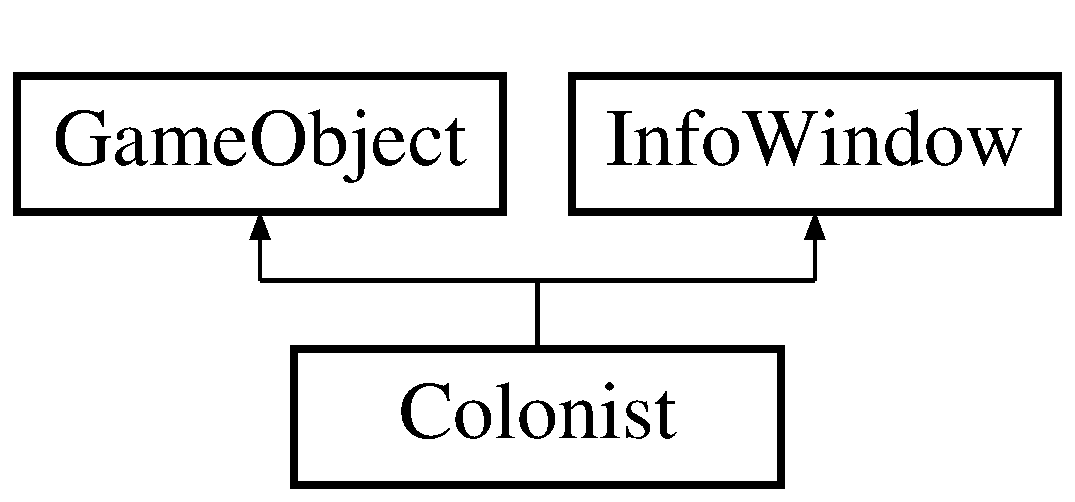
\includegraphics[height=2.000000cm]{class_colonist}
\end{center}
\end{figure}
\subsection*{Public Member Functions}
\begin{DoxyCompactItemize}
\item 
\mbox{\hyperlink{class_colonist_a6666c1c45bd7f52b423357828eaef598}{Colonist}} ()
\item 
\mbox{\hyperlink{class_colonist_a92d8c64b932a5eeeea9e873badb931cb}{$\sim$\+Colonist}} ()
\item 
int \mbox{\hyperlink{class_colonist_ae6111498494883c9509dc9f49cd2fa63}{m\+\_\+\+Create\+Colonist\+Body}} (sf\+::\+Vector2f dimentions, \mbox{\hyperlink{class_cells}{Cells}} $\ast$current\+Cell)
\item 
void \mbox{\hyperlink{class_colonist_a946c12abecdd1aa6c9be662eff8856ae}{m\+\_\+\+Assign\+Colonist\+Font}} (sf\+::\+Font \&new\+Font)
\item 
void \mbox{\hyperlink{class_colonist_a8c57004821ec2f9fc070c2f173c413e5}{m\+\_\+\+Update\+Current\+Cell}} (\mbox{\hyperlink{class_cells}{Cells}} $\ast$new\+Current\+Cell)
\item 
void \mbox{\hyperlink{class_colonist_ad51f196ece25322b1ab2a229875ac490}{m\+\_\+\+Update}} () override
\item 
void \mbox{\hyperlink{class_colonist_aef6c86dad183201cc5b4320869d73a6f}{m\+\_\+\+Update\+Info\+Window}} (sf\+::\+Vector2f view\+Lower\+Bounds, sf\+::\+Vector2f view\+Size)
\item 
void \mbox{\hyperlink{class_colonist_a5d7f2fdfe8edfbac71c00bd3f80db78b}{m\+\_\+\+Update\+Condition}} ()
\item 
void \mbox{\hyperlink{class_colonist_aa95eaa2ece608aceff02abbd69303721}{m\+\_\+\+Set\+Job}} (\mbox{\hyperlink{_colonist_8h_a7718e37d567b721003cf67cbd3125b4a}{job}} new\+Job)
\item 
void \mbox{\hyperlink{class_colonist_a9f7d167546dbc3cbbf79e9a8fdbb2c98}{m\+\_\+\+Idle\+Job}} ()
\item 
void \mbox{\hyperlink{class_colonist_a31ae6b8c4983b45489b77b92599fa971}{m\+\_\+\+Cut\+Trees}} ()
\item 
void \mbox{\hyperlink{class_colonist_ade6be47cebcac982789ba93d4bed5064}{m\+\_\+\+Build\+Building}} ()
\item 
\mbox{\hyperlink{_colonist_8h_a7718e37d567b721003cf67cbd3125b4a}{job}} \mbox{\hyperlink{class_colonist_aba477cb8f4eb974ffa72f1b519527922}{m\+\_\+\+Get\+Current\+Job}} ()
\item 
void \mbox{\hyperlink{class_colonist_acc420a406fbf716b24447baaeadb9136}{m\+\_\+\+Set\+Needed\+Wood}} (float wood\+Needed)
\item 
void \mbox{\hyperlink{class_colonist_ae7d7c74ff639334e6992142c01dd8f6f}{m\+\_\+\+Draw\+Game\+Object}} (sf\+::\+Render\+Window \&window) override
\item 
void \mbox{\hyperlink{class_colonist_a77963df06b74b1235341e235ba7b320e}{m\+\_\+\+Draw\+Filter}} (sf\+::\+Vector2f top\+Left, sf\+::\+Vector2f bottom\+Right) override
\item 
void \mbox{\hyperlink{class_colonist_a2cdc11f7d868611172ed36f67ea1393f}{m\+\_\+\+Draw\+Filter}} (sf\+::\+Vector2f top\+Left, sf\+::\+Vector2f bottom\+Right, unsigned int current\+Layer)
\item 
void \mbox{\hyperlink{class_colonist_a4dd53225a89bab611509a4d8fc0c2fb1}{m\+\_\+\+Set\+Object\+Pos}} (float x, float y) override
\item 
void \mbox{\hyperlink{class_colonist_a5baacaaf37c94daeb2a1ab21c8d9e42a}{m\+\_\+\+Set\+Current\+Layer}} (unsigned int new\+Layer)
\item 
int \mbox{\hyperlink{class_colonist_a8b03eca0f0e0cafcb2c1fd581b75b0a6}{m\+\_\+\+Get\+Current\+Layer}} ()
\item 
\mbox{\hyperlink{class_cells}{Cells}} $\ast$ \mbox{\hyperlink{class_colonist_a25bd76dec060d9bb7ee0b0d35f400443}{m\+\_\+\+Get\+Current\+Cell}} ()
\item 
void \mbox{\hyperlink{class_colonist_a350c571eddc4b145e0d05cce1668f76c}{m\+\_\+\+Follow\+Path}} ()
\item 
int \mbox{\hyperlink{class_colonist_a81892e1468ec705e99ba71c6e9ae3da3}{m\+\_\+\+Find\+New\+Path}} (\mbox{\hyperlink{class_cells}{Cells}} $\ast$end\+Cell)
\item 
void \mbox{\hyperlink{class_colonist_a87de13e9cf6d11006b46b60c220854e1}{m\+\_\+\+Assign\+Tree}} (\mbox{\hyperlink{class_wood_resource}{Wood\+Resource}} $\ast$new\+Target)
\item 
bool \mbox{\hyperlink{class_colonist_ad1a63535927eb3153249fd4081901311}{m\+\_\+\+At\+Target\+Tree}} ()
\item 
void \mbox{\hyperlink{class_colonist_a18c45b63f78136d73efcd67e92b06a73}{m\+\_\+\+Assign\+Build}} (\mbox{\hyperlink{class_building_object}{Building\+Object}} $\ast$new\+Target)
\item 
bool \mbox{\hyperlink{class_colonist_a385c46942c09d4824da79aec97ab6149}{m\+\_\+\+At\+Target\+Build}} ()
\item 
void \mbox{\hyperlink{class_colonist_ad137e98744bc418674f853a0c19d72a3}{m\+\_\+\+Reset\+Pathfinding}} ()
\item 
void \mbox{\hyperlink{class_colonist_a424fe6f992957fe97b1cc7008dfd9233}{m\+\_\+\+Set\+Interactable\+Object}} (\mbox{\hyperlink{class_building_object}{Building\+Object}} $\ast$new\+Target)
\item 
bool \mbox{\hyperlink{class_colonist_a7b5e8bd198ca9e077e9352908848e0a1}{m\+\_\+b\+At\+Interatable\+Object}} ()
\item 
bool \mbox{\hyperlink{class_colonist_a269c0b2ac4ebf5eb0fbf1286063765ff}{m\+\_\+\+Get\+Find\+New\+Path}} ()
\item 
void \mbox{\hyperlink{class_colonist_a4d5b1c31fff5922f67c8de7f5031fc5d}{m\+\_\+\+Create\+Path\+Line}} (int current\+Pos)
\item 
void \mbox{\hyperlink{class_colonist_abd0ac8d5315b88b193a0c288caa1e070}{m\+\_\+\+Select\+Colonist}} (bool selected)
\item 
bool \mbox{\hyperlink{class_colonist_ac2c3826ecc02ac228cb6c829a1ab2203}{m\+\_\+\+Get\+Selected\+Value}} ()
\end{DoxyCompactItemize}
\subsection*{Public Attributes}
\begin{DoxyCompactItemize}
\item 
bool \mbox{\hyperlink{class_colonist_a5521900ae5f26798f055c2b4a6261626}{m\+\_\+b\+Need\+Sleep}} = false
\item 
unsigned int \mbox{\hyperlink{class_colonist_a7d052b658e17e5571229eec7ae9471f7}{m\+\_\+i\+Current\+Wood}} = 0
\item 
int \mbox{\hyperlink{class_colonist_a835f8bfb0683d483f0c9ace75d9bcf59}{m\+\_\+i\+Needed\+Wood}} = 0
\item 
unsigned int \mbox{\hyperlink{class_colonist_abea3166ef031870e52518bfe83a2340b}{m\+\_\+i\+Idle\+Counter}} = 0
\end{DoxyCompactItemize}
\subsection*{Additional Inherited Members}


\subsection{Constructor \& Destructor Documentation}
\mbox{\Hypertarget{class_colonist_a6666c1c45bd7f52b423357828eaef598}\label{class_colonist_a6666c1c45bd7f52b423357828eaef598}} 
\index{Colonist@{Colonist}!Colonist@{Colonist}}
\index{Colonist@{Colonist}!Colonist@{Colonist}}
\subsubsection{\texorpdfstring{Colonist()}{Colonist()}}
{\footnotesize\ttfamily Colonist\+::\+Colonist (\begin{DoxyParamCaption}{ }\end{DoxyParamCaption})}

\mbox{\Hypertarget{class_colonist_a92d8c64b932a5eeeea9e873badb931cb}\label{class_colonist_a92d8c64b932a5eeeea9e873badb931cb}} 
\index{Colonist@{Colonist}!````~Colonist@{$\sim$\+Colonist}}
\index{````~Colonist@{$\sim$\+Colonist}!Colonist@{Colonist}}
\subsubsection{\texorpdfstring{$\sim$\+Colonist()}{~Colonist()}}
{\footnotesize\ttfamily Colonist\+::$\sim$\+Colonist (\begin{DoxyParamCaption}{ }\end{DoxyParamCaption})}



\subsection{Member Function Documentation}
\mbox{\Hypertarget{class_colonist_a18c45b63f78136d73efcd67e92b06a73}\label{class_colonist_a18c45b63f78136d73efcd67e92b06a73}} 
\index{Colonist@{Colonist}!m\+\_\+\+Assign\+Build@{m\+\_\+\+Assign\+Build}}
\index{m\+\_\+\+Assign\+Build@{m\+\_\+\+Assign\+Build}!Colonist@{Colonist}}
\subsubsection{\texorpdfstring{m\+\_\+\+Assign\+Build()}{m\_AssignBuild()}}
{\footnotesize\ttfamily void Colonist\+::m\+\_\+\+Assign\+Build (\begin{DoxyParamCaption}\item[{\mbox{\hyperlink{class_building_object}{Building\+Object}} $\ast$}]{new\+Target }\end{DoxyParamCaption})}

\mbox{\Hypertarget{class_colonist_a946c12abecdd1aa6c9be662eff8856ae}\label{class_colonist_a946c12abecdd1aa6c9be662eff8856ae}} 
\index{Colonist@{Colonist}!m\+\_\+\+Assign\+Colonist\+Font@{m\+\_\+\+Assign\+Colonist\+Font}}
\index{m\+\_\+\+Assign\+Colonist\+Font@{m\+\_\+\+Assign\+Colonist\+Font}!Colonist@{Colonist}}
\subsubsection{\texorpdfstring{m\+\_\+\+Assign\+Colonist\+Font()}{m\_AssignColonistFont()}}
{\footnotesize\ttfamily void Colonist\+::m\+\_\+\+Assign\+Colonist\+Font (\begin{DoxyParamCaption}\item[{sf\+::\+Font \&}]{new\+Font }\end{DoxyParamCaption})}

\mbox{\Hypertarget{class_colonist_a87de13e9cf6d11006b46b60c220854e1}\label{class_colonist_a87de13e9cf6d11006b46b60c220854e1}} 
\index{Colonist@{Colonist}!m\+\_\+\+Assign\+Tree@{m\+\_\+\+Assign\+Tree}}
\index{m\+\_\+\+Assign\+Tree@{m\+\_\+\+Assign\+Tree}!Colonist@{Colonist}}
\subsubsection{\texorpdfstring{m\+\_\+\+Assign\+Tree()}{m\_AssignTree()}}
{\footnotesize\ttfamily void Colonist\+::m\+\_\+\+Assign\+Tree (\begin{DoxyParamCaption}\item[{\mbox{\hyperlink{class_wood_resource}{Wood\+Resource}} $\ast$}]{new\+Target }\end{DoxyParamCaption})}

\mbox{\Hypertarget{class_colonist_a385c46942c09d4824da79aec97ab6149}\label{class_colonist_a385c46942c09d4824da79aec97ab6149}} 
\index{Colonist@{Colonist}!m\+\_\+\+At\+Target\+Build@{m\+\_\+\+At\+Target\+Build}}
\index{m\+\_\+\+At\+Target\+Build@{m\+\_\+\+At\+Target\+Build}!Colonist@{Colonist}}
\subsubsection{\texorpdfstring{m\+\_\+\+At\+Target\+Build()}{m\_AtTargetBuild()}}
{\footnotesize\ttfamily bool Colonist\+::m\+\_\+\+At\+Target\+Build (\begin{DoxyParamCaption}{ }\end{DoxyParamCaption})}

\mbox{\Hypertarget{class_colonist_ad1a63535927eb3153249fd4081901311}\label{class_colonist_ad1a63535927eb3153249fd4081901311}} 
\index{Colonist@{Colonist}!m\+\_\+\+At\+Target\+Tree@{m\+\_\+\+At\+Target\+Tree}}
\index{m\+\_\+\+At\+Target\+Tree@{m\+\_\+\+At\+Target\+Tree}!Colonist@{Colonist}}
\subsubsection{\texorpdfstring{m\+\_\+\+At\+Target\+Tree()}{m\_AtTargetTree()}}
{\footnotesize\ttfamily bool Colonist\+::m\+\_\+\+At\+Target\+Tree (\begin{DoxyParamCaption}{ }\end{DoxyParamCaption})}

\mbox{\Hypertarget{class_colonist_a7b5e8bd198ca9e077e9352908848e0a1}\label{class_colonist_a7b5e8bd198ca9e077e9352908848e0a1}} 
\index{Colonist@{Colonist}!m\+\_\+b\+At\+Interatable\+Object@{m\+\_\+b\+At\+Interatable\+Object}}
\index{m\+\_\+b\+At\+Interatable\+Object@{m\+\_\+b\+At\+Interatable\+Object}!Colonist@{Colonist}}
\subsubsection{\texorpdfstring{m\+\_\+b\+At\+Interatable\+Object()}{m\_bAtInteratableObject()}}
{\footnotesize\ttfamily bool Colonist\+::m\+\_\+b\+At\+Interatable\+Object (\begin{DoxyParamCaption}{ }\end{DoxyParamCaption})}

\mbox{\Hypertarget{class_colonist_ade6be47cebcac982789ba93d4bed5064}\label{class_colonist_ade6be47cebcac982789ba93d4bed5064}} 
\index{Colonist@{Colonist}!m\+\_\+\+Build\+Building@{m\+\_\+\+Build\+Building}}
\index{m\+\_\+\+Build\+Building@{m\+\_\+\+Build\+Building}!Colonist@{Colonist}}
\subsubsection{\texorpdfstring{m\+\_\+\+Build\+Building()}{m\_BuildBuilding()}}
{\footnotesize\ttfamily void Colonist\+::m\+\_\+\+Build\+Building (\begin{DoxyParamCaption}{ }\end{DoxyParamCaption})}

\mbox{\Hypertarget{class_colonist_ae6111498494883c9509dc9f49cd2fa63}\label{class_colonist_ae6111498494883c9509dc9f49cd2fa63}} 
\index{Colonist@{Colonist}!m\+\_\+\+Create\+Colonist\+Body@{m\+\_\+\+Create\+Colonist\+Body}}
\index{m\+\_\+\+Create\+Colonist\+Body@{m\+\_\+\+Create\+Colonist\+Body}!Colonist@{Colonist}}
\subsubsection{\texorpdfstring{m\+\_\+\+Create\+Colonist\+Body()}{m\_CreateColonistBody()}}
{\footnotesize\ttfamily int Colonist\+::m\+\_\+\+Create\+Colonist\+Body (\begin{DoxyParamCaption}\item[{sf\+::\+Vector2f}]{dimentions,  }\item[{\mbox{\hyperlink{class_cells}{Cells}} $\ast$}]{current\+Cell }\end{DoxyParamCaption})}

\mbox{\Hypertarget{class_colonist_a4d5b1c31fff5922f67c8de7f5031fc5d}\label{class_colonist_a4d5b1c31fff5922f67c8de7f5031fc5d}} 
\index{Colonist@{Colonist}!m\+\_\+\+Create\+Path\+Line@{m\+\_\+\+Create\+Path\+Line}}
\index{m\+\_\+\+Create\+Path\+Line@{m\+\_\+\+Create\+Path\+Line}!Colonist@{Colonist}}
\subsubsection{\texorpdfstring{m\+\_\+\+Create\+Path\+Line()}{m\_CreatePathLine()}}
{\footnotesize\ttfamily void Colonist\+::m\+\_\+\+Create\+Path\+Line (\begin{DoxyParamCaption}\item[{int}]{current\+Pos }\end{DoxyParamCaption})}

\mbox{\Hypertarget{class_colonist_a31ae6b8c4983b45489b77b92599fa971}\label{class_colonist_a31ae6b8c4983b45489b77b92599fa971}} 
\index{Colonist@{Colonist}!m\+\_\+\+Cut\+Trees@{m\+\_\+\+Cut\+Trees}}
\index{m\+\_\+\+Cut\+Trees@{m\+\_\+\+Cut\+Trees}!Colonist@{Colonist}}
\subsubsection{\texorpdfstring{m\+\_\+\+Cut\+Trees()}{m\_CutTrees()}}
{\footnotesize\ttfamily void Colonist\+::m\+\_\+\+Cut\+Trees (\begin{DoxyParamCaption}{ }\end{DoxyParamCaption})}

\mbox{\Hypertarget{class_colonist_a77963df06b74b1235341e235ba7b320e}\label{class_colonist_a77963df06b74b1235341e235ba7b320e}} 
\index{Colonist@{Colonist}!m\+\_\+\+Draw\+Filter@{m\+\_\+\+Draw\+Filter}}
\index{m\+\_\+\+Draw\+Filter@{m\+\_\+\+Draw\+Filter}!Colonist@{Colonist}}
\subsubsection{\texorpdfstring{m\+\_\+\+Draw\+Filter()}{m\_DrawFilter()}\hspace{0.1cm}{\footnotesize\ttfamily [1/2]}}
{\footnotesize\ttfamily void Colonist\+::m\+\_\+\+Draw\+Filter (\begin{DoxyParamCaption}\item[{sf\+::\+Vector2f}]{top\+Left,  }\item[{sf\+::\+Vector2f}]{bottom\+Right }\end{DoxyParamCaption})\hspace{0.3cm}{\ttfamily [override]}, {\ttfamily [virtual]}}



Implements \mbox{\hyperlink{class_game_object_af1a0662ca445d878b163c4648f90259c}{Game\+Object}}.

\mbox{\Hypertarget{class_colonist_a2cdc11f7d868611172ed36f67ea1393f}\label{class_colonist_a2cdc11f7d868611172ed36f67ea1393f}} 
\index{Colonist@{Colonist}!m\+\_\+\+Draw\+Filter@{m\+\_\+\+Draw\+Filter}}
\index{m\+\_\+\+Draw\+Filter@{m\+\_\+\+Draw\+Filter}!Colonist@{Colonist}}
\subsubsection{\texorpdfstring{m\+\_\+\+Draw\+Filter()}{m\_DrawFilter()}\hspace{0.1cm}{\footnotesize\ttfamily [2/2]}}
{\footnotesize\ttfamily void Colonist\+::m\+\_\+\+Draw\+Filter (\begin{DoxyParamCaption}\item[{sf\+::\+Vector2f}]{top\+Left,  }\item[{sf\+::\+Vector2f}]{bottom\+Right,  }\item[{unsigned int}]{current\+Layer }\end{DoxyParamCaption})}

\mbox{\Hypertarget{class_colonist_ae7d7c74ff639334e6992142c01dd8f6f}\label{class_colonist_ae7d7c74ff639334e6992142c01dd8f6f}} 
\index{Colonist@{Colonist}!m\+\_\+\+Draw\+Game\+Object@{m\+\_\+\+Draw\+Game\+Object}}
\index{m\+\_\+\+Draw\+Game\+Object@{m\+\_\+\+Draw\+Game\+Object}!Colonist@{Colonist}}
\subsubsection{\texorpdfstring{m\+\_\+\+Draw\+Game\+Object()}{m\_DrawGameObject()}}
{\footnotesize\ttfamily void Colonist\+::m\+\_\+\+Draw\+Game\+Object (\begin{DoxyParamCaption}\item[{sf\+::\+Render\+Window \&}]{window }\end{DoxyParamCaption})\hspace{0.3cm}{\ttfamily [override]}, {\ttfamily [virtual]}}



Implements \mbox{\hyperlink{class_game_object_a184ac59fd5167c55a54b50894e5b6721}{Game\+Object}}.

\mbox{\Hypertarget{class_colonist_a81892e1468ec705e99ba71c6e9ae3da3}\label{class_colonist_a81892e1468ec705e99ba71c6e9ae3da3}} 
\index{Colonist@{Colonist}!m\+\_\+\+Find\+New\+Path@{m\+\_\+\+Find\+New\+Path}}
\index{m\+\_\+\+Find\+New\+Path@{m\+\_\+\+Find\+New\+Path}!Colonist@{Colonist}}
\subsubsection{\texorpdfstring{m\+\_\+\+Find\+New\+Path()}{m\_FindNewPath()}}
{\footnotesize\ttfamily int Colonist\+::m\+\_\+\+Find\+New\+Path (\begin{DoxyParamCaption}\item[{\mbox{\hyperlink{class_cells}{Cells}} $\ast$}]{end\+Cell }\end{DoxyParamCaption})}

\mbox{\Hypertarget{class_colonist_a350c571eddc4b145e0d05cce1668f76c}\label{class_colonist_a350c571eddc4b145e0d05cce1668f76c}} 
\index{Colonist@{Colonist}!m\+\_\+\+Follow\+Path@{m\+\_\+\+Follow\+Path}}
\index{m\+\_\+\+Follow\+Path@{m\+\_\+\+Follow\+Path}!Colonist@{Colonist}}
\subsubsection{\texorpdfstring{m\+\_\+\+Follow\+Path()}{m\_FollowPath()}}
{\footnotesize\ttfamily void Colonist\+::m\+\_\+\+Follow\+Path (\begin{DoxyParamCaption}{ }\end{DoxyParamCaption})}

\mbox{\Hypertarget{class_colonist_a25bd76dec060d9bb7ee0b0d35f400443}\label{class_colonist_a25bd76dec060d9bb7ee0b0d35f400443}} 
\index{Colonist@{Colonist}!m\+\_\+\+Get\+Current\+Cell@{m\+\_\+\+Get\+Current\+Cell}}
\index{m\+\_\+\+Get\+Current\+Cell@{m\+\_\+\+Get\+Current\+Cell}!Colonist@{Colonist}}
\subsubsection{\texorpdfstring{m\+\_\+\+Get\+Current\+Cell()}{m\_GetCurrentCell()}}
{\footnotesize\ttfamily \mbox{\hyperlink{class_cells}{Cells}}$\ast$ Colonist\+::m\+\_\+\+Get\+Current\+Cell (\begin{DoxyParamCaption}{ }\end{DoxyParamCaption})}

\mbox{\Hypertarget{class_colonist_aba477cb8f4eb974ffa72f1b519527922}\label{class_colonist_aba477cb8f4eb974ffa72f1b519527922}} 
\index{Colonist@{Colonist}!m\+\_\+\+Get\+Current\+Job@{m\+\_\+\+Get\+Current\+Job}}
\index{m\+\_\+\+Get\+Current\+Job@{m\+\_\+\+Get\+Current\+Job}!Colonist@{Colonist}}
\subsubsection{\texorpdfstring{m\+\_\+\+Get\+Current\+Job()}{m\_GetCurrentJob()}}
{\footnotesize\ttfamily \mbox{\hyperlink{_colonist_8h_a7718e37d567b721003cf67cbd3125b4a}{job}} Colonist\+::m\+\_\+\+Get\+Current\+Job (\begin{DoxyParamCaption}{ }\end{DoxyParamCaption})}

\mbox{\Hypertarget{class_colonist_a8b03eca0f0e0cafcb2c1fd581b75b0a6}\label{class_colonist_a8b03eca0f0e0cafcb2c1fd581b75b0a6}} 
\index{Colonist@{Colonist}!m\+\_\+\+Get\+Current\+Layer@{m\+\_\+\+Get\+Current\+Layer}}
\index{m\+\_\+\+Get\+Current\+Layer@{m\+\_\+\+Get\+Current\+Layer}!Colonist@{Colonist}}
\subsubsection{\texorpdfstring{m\+\_\+\+Get\+Current\+Layer()}{m\_GetCurrentLayer()}}
{\footnotesize\ttfamily int Colonist\+::m\+\_\+\+Get\+Current\+Layer (\begin{DoxyParamCaption}{ }\end{DoxyParamCaption})}

\mbox{\Hypertarget{class_colonist_a269c0b2ac4ebf5eb0fbf1286063765ff}\label{class_colonist_a269c0b2ac4ebf5eb0fbf1286063765ff}} 
\index{Colonist@{Colonist}!m\+\_\+\+Get\+Find\+New\+Path@{m\+\_\+\+Get\+Find\+New\+Path}}
\index{m\+\_\+\+Get\+Find\+New\+Path@{m\+\_\+\+Get\+Find\+New\+Path}!Colonist@{Colonist}}
\subsubsection{\texorpdfstring{m\+\_\+\+Get\+Find\+New\+Path()}{m\_GetFindNewPath()}}
{\footnotesize\ttfamily bool Colonist\+::m\+\_\+\+Get\+Find\+New\+Path (\begin{DoxyParamCaption}{ }\end{DoxyParamCaption})}

\mbox{\Hypertarget{class_colonist_ac2c3826ecc02ac228cb6c829a1ab2203}\label{class_colonist_ac2c3826ecc02ac228cb6c829a1ab2203}} 
\index{Colonist@{Colonist}!m\+\_\+\+Get\+Selected\+Value@{m\+\_\+\+Get\+Selected\+Value}}
\index{m\+\_\+\+Get\+Selected\+Value@{m\+\_\+\+Get\+Selected\+Value}!Colonist@{Colonist}}
\subsubsection{\texorpdfstring{m\+\_\+\+Get\+Selected\+Value()}{m\_GetSelectedValue()}}
{\footnotesize\ttfamily bool Colonist\+::m\+\_\+\+Get\+Selected\+Value (\begin{DoxyParamCaption}{ }\end{DoxyParamCaption})}

\mbox{\Hypertarget{class_colonist_a9f7d167546dbc3cbbf79e9a8fdbb2c98}\label{class_colonist_a9f7d167546dbc3cbbf79e9a8fdbb2c98}} 
\index{Colonist@{Colonist}!m\+\_\+\+Idle\+Job@{m\+\_\+\+Idle\+Job}}
\index{m\+\_\+\+Idle\+Job@{m\+\_\+\+Idle\+Job}!Colonist@{Colonist}}
\subsubsection{\texorpdfstring{m\+\_\+\+Idle\+Job()}{m\_IdleJob()}}
{\footnotesize\ttfamily void Colonist\+::m\+\_\+\+Idle\+Job (\begin{DoxyParamCaption}{ }\end{DoxyParamCaption})}

\mbox{\Hypertarget{class_colonist_ad137e98744bc418674f853a0c19d72a3}\label{class_colonist_ad137e98744bc418674f853a0c19d72a3}} 
\index{Colonist@{Colonist}!m\+\_\+\+Reset\+Pathfinding@{m\+\_\+\+Reset\+Pathfinding}}
\index{m\+\_\+\+Reset\+Pathfinding@{m\+\_\+\+Reset\+Pathfinding}!Colonist@{Colonist}}
\subsubsection{\texorpdfstring{m\+\_\+\+Reset\+Pathfinding()}{m\_ResetPathfinding()}}
{\footnotesize\ttfamily void Colonist\+::m\+\_\+\+Reset\+Pathfinding (\begin{DoxyParamCaption}{ }\end{DoxyParamCaption})}

\mbox{\Hypertarget{class_colonist_abd0ac8d5315b88b193a0c288caa1e070}\label{class_colonist_abd0ac8d5315b88b193a0c288caa1e070}} 
\index{Colonist@{Colonist}!m\+\_\+\+Select\+Colonist@{m\+\_\+\+Select\+Colonist}}
\index{m\+\_\+\+Select\+Colonist@{m\+\_\+\+Select\+Colonist}!Colonist@{Colonist}}
\subsubsection{\texorpdfstring{m\+\_\+\+Select\+Colonist()}{m\_SelectColonist()}}
{\footnotesize\ttfamily void Colonist\+::m\+\_\+\+Select\+Colonist (\begin{DoxyParamCaption}\item[{bool}]{selected }\end{DoxyParamCaption})}

\mbox{\Hypertarget{class_colonist_a5baacaaf37c94daeb2a1ab21c8d9e42a}\label{class_colonist_a5baacaaf37c94daeb2a1ab21c8d9e42a}} 
\index{Colonist@{Colonist}!m\+\_\+\+Set\+Current\+Layer@{m\+\_\+\+Set\+Current\+Layer}}
\index{m\+\_\+\+Set\+Current\+Layer@{m\+\_\+\+Set\+Current\+Layer}!Colonist@{Colonist}}
\subsubsection{\texorpdfstring{m\+\_\+\+Set\+Current\+Layer()}{m\_SetCurrentLayer()}}
{\footnotesize\ttfamily void Colonist\+::m\+\_\+\+Set\+Current\+Layer (\begin{DoxyParamCaption}\item[{unsigned int}]{new\+Layer }\end{DoxyParamCaption})}

\mbox{\Hypertarget{class_colonist_a424fe6f992957fe97b1cc7008dfd9233}\label{class_colonist_a424fe6f992957fe97b1cc7008dfd9233}} 
\index{Colonist@{Colonist}!m\+\_\+\+Set\+Interactable\+Object@{m\+\_\+\+Set\+Interactable\+Object}}
\index{m\+\_\+\+Set\+Interactable\+Object@{m\+\_\+\+Set\+Interactable\+Object}!Colonist@{Colonist}}
\subsubsection{\texorpdfstring{m\+\_\+\+Set\+Interactable\+Object()}{m\_SetInteractableObject()}}
{\footnotesize\ttfamily void Colonist\+::m\+\_\+\+Set\+Interactable\+Object (\begin{DoxyParamCaption}\item[{\mbox{\hyperlink{class_building_object}{Building\+Object}} $\ast$}]{new\+Target }\end{DoxyParamCaption})}

\mbox{\Hypertarget{class_colonist_aa95eaa2ece608aceff02abbd69303721}\label{class_colonist_aa95eaa2ece608aceff02abbd69303721}} 
\index{Colonist@{Colonist}!m\+\_\+\+Set\+Job@{m\+\_\+\+Set\+Job}}
\index{m\+\_\+\+Set\+Job@{m\+\_\+\+Set\+Job}!Colonist@{Colonist}}
\subsubsection{\texorpdfstring{m\+\_\+\+Set\+Job()}{m\_SetJob()}}
{\footnotesize\ttfamily void Colonist\+::m\+\_\+\+Set\+Job (\begin{DoxyParamCaption}\item[{\mbox{\hyperlink{_colonist_8h_a7718e37d567b721003cf67cbd3125b4a}{job}}}]{new\+Job }\end{DoxyParamCaption})}

\mbox{\Hypertarget{class_colonist_acc420a406fbf716b24447baaeadb9136}\label{class_colonist_acc420a406fbf716b24447baaeadb9136}} 
\index{Colonist@{Colonist}!m\+\_\+\+Set\+Needed\+Wood@{m\+\_\+\+Set\+Needed\+Wood}}
\index{m\+\_\+\+Set\+Needed\+Wood@{m\+\_\+\+Set\+Needed\+Wood}!Colonist@{Colonist}}
\subsubsection{\texorpdfstring{m\+\_\+\+Set\+Needed\+Wood()}{m\_SetNeededWood()}}
{\footnotesize\ttfamily void Colonist\+::m\+\_\+\+Set\+Needed\+Wood (\begin{DoxyParamCaption}\item[{float}]{wood\+Needed }\end{DoxyParamCaption})}

\mbox{\Hypertarget{class_colonist_a4dd53225a89bab611509a4d8fc0c2fb1}\label{class_colonist_a4dd53225a89bab611509a4d8fc0c2fb1}} 
\index{Colonist@{Colonist}!m\+\_\+\+Set\+Object\+Pos@{m\+\_\+\+Set\+Object\+Pos}}
\index{m\+\_\+\+Set\+Object\+Pos@{m\+\_\+\+Set\+Object\+Pos}!Colonist@{Colonist}}
\subsubsection{\texorpdfstring{m\+\_\+\+Set\+Object\+Pos()}{m\_SetObjectPos()}}
{\footnotesize\ttfamily void Colonist\+::m\+\_\+\+Set\+Object\+Pos (\begin{DoxyParamCaption}\item[{float}]{x,  }\item[{float}]{y }\end{DoxyParamCaption})\hspace{0.3cm}{\ttfamily [override]}, {\ttfamily [virtual]}}



Implements \mbox{\hyperlink{class_game_object_ad1f8ea8eb3673b1af8215bf92cdc0df8}{Game\+Object}}.

\mbox{\Hypertarget{class_colonist_ad51f196ece25322b1ab2a229875ac490}\label{class_colonist_ad51f196ece25322b1ab2a229875ac490}} 
\index{Colonist@{Colonist}!m\+\_\+\+Update@{m\+\_\+\+Update}}
\index{m\+\_\+\+Update@{m\+\_\+\+Update}!Colonist@{Colonist}}
\subsubsection{\texorpdfstring{m\+\_\+\+Update()}{m\_Update()}}
{\footnotesize\ttfamily void Colonist\+::m\+\_\+\+Update (\begin{DoxyParamCaption}{ }\end{DoxyParamCaption})\hspace{0.3cm}{\ttfamily [override]}, {\ttfamily [virtual]}}



Implements \mbox{\hyperlink{class_game_object_a3af5a7b470e09f13a1422439fc6a9ba8}{Game\+Object}}.

\mbox{\Hypertarget{class_colonist_a5d7f2fdfe8edfbac71c00bd3f80db78b}\label{class_colonist_a5d7f2fdfe8edfbac71c00bd3f80db78b}} 
\index{Colonist@{Colonist}!m\+\_\+\+Update\+Condition@{m\+\_\+\+Update\+Condition}}
\index{m\+\_\+\+Update\+Condition@{m\+\_\+\+Update\+Condition}!Colonist@{Colonist}}
\subsubsection{\texorpdfstring{m\+\_\+\+Update\+Condition()}{m\_UpdateCondition()}}
{\footnotesize\ttfamily void Colonist\+::m\+\_\+\+Update\+Condition (\begin{DoxyParamCaption}{ }\end{DoxyParamCaption})}

\mbox{\Hypertarget{class_colonist_a8c57004821ec2f9fc070c2f173c413e5}\label{class_colonist_a8c57004821ec2f9fc070c2f173c413e5}} 
\index{Colonist@{Colonist}!m\+\_\+\+Update\+Current\+Cell@{m\+\_\+\+Update\+Current\+Cell}}
\index{m\+\_\+\+Update\+Current\+Cell@{m\+\_\+\+Update\+Current\+Cell}!Colonist@{Colonist}}
\subsubsection{\texorpdfstring{m\+\_\+\+Update\+Current\+Cell()}{m\_UpdateCurrentCell()}}
{\footnotesize\ttfamily void Colonist\+::m\+\_\+\+Update\+Current\+Cell (\begin{DoxyParamCaption}\item[{\mbox{\hyperlink{class_cells}{Cells}} $\ast$}]{new\+Current\+Cell }\end{DoxyParamCaption})}

\mbox{\Hypertarget{class_colonist_aef6c86dad183201cc5b4320869d73a6f}\label{class_colonist_aef6c86dad183201cc5b4320869d73a6f}} 
\index{Colonist@{Colonist}!m\+\_\+\+Update\+Info\+Window@{m\+\_\+\+Update\+Info\+Window}}
\index{m\+\_\+\+Update\+Info\+Window@{m\+\_\+\+Update\+Info\+Window}!Colonist@{Colonist}}
\subsubsection{\texorpdfstring{m\+\_\+\+Update\+Info\+Window()}{m\_UpdateInfoWindow()}}
{\footnotesize\ttfamily void Colonist\+::m\+\_\+\+Update\+Info\+Window (\begin{DoxyParamCaption}\item[{sf\+::\+Vector2f}]{view\+Lower\+Bounds,  }\item[{sf\+::\+Vector2f}]{view\+Size }\end{DoxyParamCaption})}



\subsection{Member Data Documentation}
\mbox{\Hypertarget{class_colonist_a5521900ae5f26798f055c2b4a6261626}\label{class_colonist_a5521900ae5f26798f055c2b4a6261626}} 
\index{Colonist@{Colonist}!m\+\_\+b\+Need\+Sleep@{m\+\_\+b\+Need\+Sleep}}
\index{m\+\_\+b\+Need\+Sleep@{m\+\_\+b\+Need\+Sleep}!Colonist@{Colonist}}
\subsubsection{\texorpdfstring{m\+\_\+b\+Need\+Sleep}{m\_bNeedSleep}}
{\footnotesize\ttfamily bool Colonist\+::m\+\_\+b\+Need\+Sleep = false}

\mbox{\Hypertarget{class_colonist_a7d052b658e17e5571229eec7ae9471f7}\label{class_colonist_a7d052b658e17e5571229eec7ae9471f7}} 
\index{Colonist@{Colonist}!m\+\_\+i\+Current\+Wood@{m\+\_\+i\+Current\+Wood}}
\index{m\+\_\+i\+Current\+Wood@{m\+\_\+i\+Current\+Wood}!Colonist@{Colonist}}
\subsubsection{\texorpdfstring{m\+\_\+i\+Current\+Wood}{m\_iCurrentWood}}
{\footnotesize\ttfamily unsigned int Colonist\+::m\+\_\+i\+Current\+Wood = 0}

\mbox{\Hypertarget{class_colonist_abea3166ef031870e52518bfe83a2340b}\label{class_colonist_abea3166ef031870e52518bfe83a2340b}} 
\index{Colonist@{Colonist}!m\+\_\+i\+Idle\+Counter@{m\+\_\+i\+Idle\+Counter}}
\index{m\+\_\+i\+Idle\+Counter@{m\+\_\+i\+Idle\+Counter}!Colonist@{Colonist}}
\subsubsection{\texorpdfstring{m\+\_\+i\+Idle\+Counter}{m\_iIdleCounter}}
{\footnotesize\ttfamily unsigned int Colonist\+::m\+\_\+i\+Idle\+Counter = 0}

\mbox{\Hypertarget{class_colonist_a835f8bfb0683d483f0c9ace75d9bcf59}\label{class_colonist_a835f8bfb0683d483f0c9ace75d9bcf59}} 
\index{Colonist@{Colonist}!m\+\_\+i\+Needed\+Wood@{m\+\_\+i\+Needed\+Wood}}
\index{m\+\_\+i\+Needed\+Wood@{m\+\_\+i\+Needed\+Wood}!Colonist@{Colonist}}
\subsubsection{\texorpdfstring{m\+\_\+i\+Needed\+Wood}{m\_iNeededWood}}
{\footnotesize\ttfamily int Colonist\+::m\+\_\+i\+Needed\+Wood = 0}



The documentation for this class was generated from the following file\+:\begin{DoxyCompactItemize}
\item 
inc/\mbox{\hyperlink{_colonist_8h}{Colonist.\+h}}\end{DoxyCompactItemize}

\hypertarget{class_colonist_manager}{}\section{Colonist\+Manager Class Reference}
\label{class_colonist_manager}\index{Colonist\+Manager@{Colonist\+Manager}}


{\ttfamily \#include $<$Colonist\+Manager.\+h$>$}

\subsection*{Public Member Functions}
\begin{DoxyCompactItemize}
\item 
\mbox{\hyperlink{class_colonist_manager_ae4103d1c28b871155a10f8df08974c7e}{Colonist\+Manager}} ()
\item 
\mbox{\hyperlink{class_colonist_manager_a33c8e31a0646e00653ce25c06f7e5038}{$\sim$\+Colonist\+Manager}} ()
\item 
void \mbox{\hyperlink{class_colonist_manager_a068d45eb539d9349c00771208c019187}{m\+\_\+\+Add\+Colonist}} (int number\+Of\+Colonists, sf\+::\+Vector2f dimentions, \mbox{\hyperlink{class_grid}{Grid}} \&current\+Grid, int starting\+Layer)
\item 
void \mbox{\hyperlink{class_colonist_manager_a67277f61ffb7e5e37657107088770041}{m\+\_\+\+Assign\+Colonist\+Fonts}} (sf\+::\+Font \&new\+Font)
\item 
void \mbox{\hyperlink{class_colonist_manager_a27e8588e8f4c341ea31d92cb122440bb}{m\+\_\+\+Update}} (\mbox{\hyperlink{class_grid}{Grid}} \&Current\+Grid)
\item 
void \mbox{\hyperlink{class_colonist_manager_abd1e80e0f01891857d81300eed3347f4}{m\+\_\+\+Update\+Info\+Windows}} (sf\+::\+Vector2f view\+Lower\+Bounds, sf\+::\+Vector2f view\+Size)
\item 
void \mbox{\hyperlink{class_colonist_manager_a4ae7bcfdb32a8862d950f36d357145dc}{m\+\_\+\+Pathfinding}} (\mbox{\hyperlink{class_grid}{Grid}} \&Current\+Grid, \mbox{\hyperlink{class_resource_management}{Resource\+Management}} \&current\+Manager)
\item 
void \mbox{\hyperlink{class_colonist_manager_a3c6476b726ac4ccf91be332be262810a}{m\+\_\+\+Pathfinding}} (\mbox{\hyperlink{class_grid}{Grid}} \&Current\+Grid, \mbox{\hyperlink{class_resource_management}{Resource\+Management}} \&resource\+Manager, \mbox{\hyperlink{class_building_manager}{Building\+Manager}} \&building\+Manager)
\item 
void \mbox{\hyperlink{class_colonist_manager_a03bf090e3d6dc4f731daef7f91ea1f11}{m\+\_\+\+Render}} (sf\+::\+Render\+Window \&window)
\item 
void \mbox{\hyperlink{class_colonist_manager_ae7960d47970d69bc0f2f3de15321fa90}{m\+\_\+\+Draw\+Filter}} (sf\+::\+Vector2f top\+Left, sf\+::\+Vector2f bottom\+Right)
\item 
void \mbox{\hyperlink{class_colonist_manager_a1cfc018393b4410129875a3fe0be4fd4}{m\+\_\+\+Draw\+Filter}} (sf\+::\+Vector2f top\+Left, sf\+::\+Vector2f bottom\+Right, unsigned int current\+Layer)
\item 
void \mbox{\hyperlink{class_colonist_manager_adb2f8be8fad5170fb41385c6a62a0ba5}{m\+\_\+\+Select\+Colonist}} (sf\+::\+Vector2f top\+Left, sf\+::\+Vector2f bottom\+Right, bool mouse\+Down)
\item 
void \mbox{\hyperlink{class_colonist_manager_ac21585da4afdb19b5b5474c630960189}{m\+\_\+\+Check\+For\+Selected}} ()
\item 
void \mbox{\hyperlink{class_colonist_manager_a8a9cb88c826c72026575e5c2d9bec88d}{m\+\_\+\+Set\+Colonist\+Idle}} ()
\item 
void \mbox{\hyperlink{class_colonist_manager_ad494974bebe1f0af43b2721f289f7772}{m\+\_\+\+Set\+Colonist\+Tree\+Cut}} ()
\item 
void \mbox{\hyperlink{class_colonist_manager_a64d61e7131db646318691539f0460eed}{m\+\_\+\+Set\+Colonist\+Construction}} ()
\item 
void \mbox{\hyperlink{class_colonist_manager_ab3101b874a6411a4929a7238200e1599}{m\+\_\+\+Create\+Colonist\+Action\+Buttons}} (sf\+::\+Font game\+Font, sf\+::\+Render\+Window \&window)
\item 
std\+::vector$<$ tgui\+::\+Button\+::\+Ptr $>$ \mbox{\hyperlink{class_colonist_manager_abcfd2d4b02e3acc1baa932b72f84f9eb}{m\+\_\+\+Get\+Colonist\+Buttons}} ()
\end{DoxyCompactItemize}
\subsection*{Public Attributes}
\begin{DoxyCompactItemize}
\item 
bool \mbox{\hyperlink{class_colonist_manager_a0b3bc58666c4a5064db8227f3c92cf64}{m\+\_\+b\+Colonist\+Selected}} = false
\item 
bool \mbox{\hyperlink{class_colonist_manager_a62044d795d70510931bbcfb3100267be}{m\+\_\+b\+Buttons\+Created}} = false
\item 
bool \mbox{\hyperlink{class_colonist_manager_a8d9b925d50fd4cbedba3685f4471fbe2}{m\+\_\+b\+Buttons\+Removed}} = false
\item 
std\+::vector$<$ tgui\+::\+Button\+::\+Ptr $>$ \mbox{\hyperlink{class_colonist_manager_a450c58b087a8c44286bddacf36c51811}{v\+\_\+\+List\+Of\+Buttons}}
\end{DoxyCompactItemize}


\subsection{Constructor \& Destructor Documentation}
\mbox{\Hypertarget{class_colonist_manager_ae4103d1c28b871155a10f8df08974c7e}\label{class_colonist_manager_ae4103d1c28b871155a10f8df08974c7e}} 
\index{Colonist\+Manager@{Colonist\+Manager}!Colonist\+Manager@{Colonist\+Manager}}
\index{Colonist\+Manager@{Colonist\+Manager}!Colonist\+Manager@{Colonist\+Manager}}
\subsubsection{\texorpdfstring{Colonist\+Manager()}{ColonistManager()}}
{\footnotesize\ttfamily Colonist\+Manager\+::\+Colonist\+Manager (\begin{DoxyParamCaption}{ }\end{DoxyParamCaption})}

\mbox{\Hypertarget{class_colonist_manager_a33c8e31a0646e00653ce25c06f7e5038}\label{class_colonist_manager_a33c8e31a0646e00653ce25c06f7e5038}} 
\index{Colonist\+Manager@{Colonist\+Manager}!````~Colonist\+Manager@{$\sim$\+Colonist\+Manager}}
\index{````~Colonist\+Manager@{$\sim$\+Colonist\+Manager}!Colonist\+Manager@{Colonist\+Manager}}
\subsubsection{\texorpdfstring{$\sim$\+Colonist\+Manager()}{~ColonistManager()}}
{\footnotesize\ttfamily Colonist\+Manager\+::$\sim$\+Colonist\+Manager (\begin{DoxyParamCaption}{ }\end{DoxyParamCaption})}



\subsection{Member Function Documentation}
\mbox{\Hypertarget{class_colonist_manager_a068d45eb539d9349c00771208c019187}\label{class_colonist_manager_a068d45eb539d9349c00771208c019187}} 
\index{Colonist\+Manager@{Colonist\+Manager}!m\+\_\+\+Add\+Colonist@{m\+\_\+\+Add\+Colonist}}
\index{m\+\_\+\+Add\+Colonist@{m\+\_\+\+Add\+Colonist}!Colonist\+Manager@{Colonist\+Manager}}
\subsubsection{\texorpdfstring{m\+\_\+\+Add\+Colonist()}{m\_AddColonist()}}
{\footnotesize\ttfamily void Colonist\+Manager\+::m\+\_\+\+Add\+Colonist (\begin{DoxyParamCaption}\item[{int}]{number\+Of\+Colonists,  }\item[{sf\+::\+Vector2f}]{dimentions,  }\item[{\mbox{\hyperlink{class_grid}{Grid}} \&}]{current\+Grid,  }\item[{int}]{starting\+Layer }\end{DoxyParamCaption})}

\mbox{\Hypertarget{class_colonist_manager_a67277f61ffb7e5e37657107088770041}\label{class_colonist_manager_a67277f61ffb7e5e37657107088770041}} 
\index{Colonist\+Manager@{Colonist\+Manager}!m\+\_\+\+Assign\+Colonist\+Fonts@{m\+\_\+\+Assign\+Colonist\+Fonts}}
\index{m\+\_\+\+Assign\+Colonist\+Fonts@{m\+\_\+\+Assign\+Colonist\+Fonts}!Colonist\+Manager@{Colonist\+Manager}}
\subsubsection{\texorpdfstring{m\+\_\+\+Assign\+Colonist\+Fonts()}{m\_AssignColonistFonts()}}
{\footnotesize\ttfamily void Colonist\+Manager\+::m\+\_\+\+Assign\+Colonist\+Fonts (\begin{DoxyParamCaption}\item[{sf\+::\+Font \&}]{new\+Font }\end{DoxyParamCaption})}

\mbox{\Hypertarget{class_colonist_manager_ac21585da4afdb19b5b5474c630960189}\label{class_colonist_manager_ac21585da4afdb19b5b5474c630960189}} 
\index{Colonist\+Manager@{Colonist\+Manager}!m\+\_\+\+Check\+For\+Selected@{m\+\_\+\+Check\+For\+Selected}}
\index{m\+\_\+\+Check\+For\+Selected@{m\+\_\+\+Check\+For\+Selected}!Colonist\+Manager@{Colonist\+Manager}}
\subsubsection{\texorpdfstring{m\+\_\+\+Check\+For\+Selected()}{m\_CheckForSelected()}}
{\footnotesize\ttfamily void Colonist\+Manager\+::m\+\_\+\+Check\+For\+Selected (\begin{DoxyParamCaption}{ }\end{DoxyParamCaption})}

\mbox{\Hypertarget{class_colonist_manager_ab3101b874a6411a4929a7238200e1599}\label{class_colonist_manager_ab3101b874a6411a4929a7238200e1599}} 
\index{Colonist\+Manager@{Colonist\+Manager}!m\+\_\+\+Create\+Colonist\+Action\+Buttons@{m\+\_\+\+Create\+Colonist\+Action\+Buttons}}
\index{m\+\_\+\+Create\+Colonist\+Action\+Buttons@{m\+\_\+\+Create\+Colonist\+Action\+Buttons}!Colonist\+Manager@{Colonist\+Manager}}
\subsubsection{\texorpdfstring{m\+\_\+\+Create\+Colonist\+Action\+Buttons()}{m\_CreateColonistActionButtons()}}
{\footnotesize\ttfamily void Colonist\+Manager\+::m\+\_\+\+Create\+Colonist\+Action\+Buttons (\begin{DoxyParamCaption}\item[{sf\+::\+Font}]{game\+Font,  }\item[{sf\+::\+Render\+Window \&}]{window }\end{DoxyParamCaption})}

\mbox{\Hypertarget{class_colonist_manager_ae7960d47970d69bc0f2f3de15321fa90}\label{class_colonist_manager_ae7960d47970d69bc0f2f3de15321fa90}} 
\index{Colonist\+Manager@{Colonist\+Manager}!m\+\_\+\+Draw\+Filter@{m\+\_\+\+Draw\+Filter}}
\index{m\+\_\+\+Draw\+Filter@{m\+\_\+\+Draw\+Filter}!Colonist\+Manager@{Colonist\+Manager}}
\subsubsection{\texorpdfstring{m\+\_\+\+Draw\+Filter()}{m\_DrawFilter()}\hspace{0.1cm}{\footnotesize\ttfamily [1/2]}}
{\footnotesize\ttfamily void Colonist\+Manager\+::m\+\_\+\+Draw\+Filter (\begin{DoxyParamCaption}\item[{sf\+::\+Vector2f}]{top\+Left,  }\item[{sf\+::\+Vector2f}]{bottom\+Right }\end{DoxyParamCaption})}

\mbox{\Hypertarget{class_colonist_manager_a1cfc018393b4410129875a3fe0be4fd4}\label{class_colonist_manager_a1cfc018393b4410129875a3fe0be4fd4}} 
\index{Colonist\+Manager@{Colonist\+Manager}!m\+\_\+\+Draw\+Filter@{m\+\_\+\+Draw\+Filter}}
\index{m\+\_\+\+Draw\+Filter@{m\+\_\+\+Draw\+Filter}!Colonist\+Manager@{Colonist\+Manager}}
\subsubsection{\texorpdfstring{m\+\_\+\+Draw\+Filter()}{m\_DrawFilter()}\hspace{0.1cm}{\footnotesize\ttfamily [2/2]}}
{\footnotesize\ttfamily void Colonist\+Manager\+::m\+\_\+\+Draw\+Filter (\begin{DoxyParamCaption}\item[{sf\+::\+Vector2f}]{top\+Left,  }\item[{sf\+::\+Vector2f}]{bottom\+Right,  }\item[{unsigned int}]{current\+Layer }\end{DoxyParamCaption})}

\mbox{\Hypertarget{class_colonist_manager_abcfd2d4b02e3acc1baa932b72f84f9eb}\label{class_colonist_manager_abcfd2d4b02e3acc1baa932b72f84f9eb}} 
\index{Colonist\+Manager@{Colonist\+Manager}!m\+\_\+\+Get\+Colonist\+Buttons@{m\+\_\+\+Get\+Colonist\+Buttons}}
\index{m\+\_\+\+Get\+Colonist\+Buttons@{m\+\_\+\+Get\+Colonist\+Buttons}!Colonist\+Manager@{Colonist\+Manager}}
\subsubsection{\texorpdfstring{m\+\_\+\+Get\+Colonist\+Buttons()}{m\_GetColonistButtons()}}
{\footnotesize\ttfamily std\+::vector$<$tgui\+::\+Button\+::\+Ptr$>$ Colonist\+Manager\+::m\+\_\+\+Get\+Colonist\+Buttons (\begin{DoxyParamCaption}{ }\end{DoxyParamCaption})}

\mbox{\Hypertarget{class_colonist_manager_a4ae7bcfdb32a8862d950f36d357145dc}\label{class_colonist_manager_a4ae7bcfdb32a8862d950f36d357145dc}} 
\index{Colonist\+Manager@{Colonist\+Manager}!m\+\_\+\+Pathfinding@{m\+\_\+\+Pathfinding}}
\index{m\+\_\+\+Pathfinding@{m\+\_\+\+Pathfinding}!Colonist\+Manager@{Colonist\+Manager}}
\subsubsection{\texorpdfstring{m\+\_\+\+Pathfinding()}{m\_Pathfinding()}\hspace{0.1cm}{\footnotesize\ttfamily [1/2]}}
{\footnotesize\ttfamily void Colonist\+Manager\+::m\+\_\+\+Pathfinding (\begin{DoxyParamCaption}\item[{\mbox{\hyperlink{class_grid}{Grid}} \&}]{Current\+Grid,  }\item[{\mbox{\hyperlink{class_resource_management}{Resource\+Management}} \&}]{current\+Manager }\end{DoxyParamCaption})}

\mbox{\Hypertarget{class_colonist_manager_a3c6476b726ac4ccf91be332be262810a}\label{class_colonist_manager_a3c6476b726ac4ccf91be332be262810a}} 
\index{Colonist\+Manager@{Colonist\+Manager}!m\+\_\+\+Pathfinding@{m\+\_\+\+Pathfinding}}
\index{m\+\_\+\+Pathfinding@{m\+\_\+\+Pathfinding}!Colonist\+Manager@{Colonist\+Manager}}
\subsubsection{\texorpdfstring{m\+\_\+\+Pathfinding()}{m\_Pathfinding()}\hspace{0.1cm}{\footnotesize\ttfamily [2/2]}}
{\footnotesize\ttfamily void Colonist\+Manager\+::m\+\_\+\+Pathfinding (\begin{DoxyParamCaption}\item[{\mbox{\hyperlink{class_grid}{Grid}} \&}]{Current\+Grid,  }\item[{\mbox{\hyperlink{class_resource_management}{Resource\+Management}} \&}]{resource\+Manager,  }\item[{\mbox{\hyperlink{class_building_manager}{Building\+Manager}} \&}]{building\+Manager }\end{DoxyParamCaption})}

\mbox{\Hypertarget{class_colonist_manager_a03bf090e3d6dc4f731daef7f91ea1f11}\label{class_colonist_manager_a03bf090e3d6dc4f731daef7f91ea1f11}} 
\index{Colonist\+Manager@{Colonist\+Manager}!m\+\_\+\+Render@{m\+\_\+\+Render}}
\index{m\+\_\+\+Render@{m\+\_\+\+Render}!Colonist\+Manager@{Colonist\+Manager}}
\subsubsection{\texorpdfstring{m\+\_\+\+Render()}{m\_Render()}}
{\footnotesize\ttfamily void Colonist\+Manager\+::m\+\_\+\+Render (\begin{DoxyParamCaption}\item[{sf\+::\+Render\+Window \&}]{window }\end{DoxyParamCaption})}

\mbox{\Hypertarget{class_colonist_manager_adb2f8be8fad5170fb41385c6a62a0ba5}\label{class_colonist_manager_adb2f8be8fad5170fb41385c6a62a0ba5}} 
\index{Colonist\+Manager@{Colonist\+Manager}!m\+\_\+\+Select\+Colonist@{m\+\_\+\+Select\+Colonist}}
\index{m\+\_\+\+Select\+Colonist@{m\+\_\+\+Select\+Colonist}!Colonist\+Manager@{Colonist\+Manager}}
\subsubsection{\texorpdfstring{m\+\_\+\+Select\+Colonist()}{m\_SelectColonist()}}
{\footnotesize\ttfamily void Colonist\+Manager\+::m\+\_\+\+Select\+Colonist (\begin{DoxyParamCaption}\item[{sf\+::\+Vector2f}]{top\+Left,  }\item[{sf\+::\+Vector2f}]{bottom\+Right,  }\item[{bool}]{mouse\+Down }\end{DoxyParamCaption})}

\mbox{\Hypertarget{class_colonist_manager_a64d61e7131db646318691539f0460eed}\label{class_colonist_manager_a64d61e7131db646318691539f0460eed}} 
\index{Colonist\+Manager@{Colonist\+Manager}!m\+\_\+\+Set\+Colonist\+Construction@{m\+\_\+\+Set\+Colonist\+Construction}}
\index{m\+\_\+\+Set\+Colonist\+Construction@{m\+\_\+\+Set\+Colonist\+Construction}!Colonist\+Manager@{Colonist\+Manager}}
\subsubsection{\texorpdfstring{m\+\_\+\+Set\+Colonist\+Construction()}{m\_SetColonistConstruction()}}
{\footnotesize\ttfamily void Colonist\+Manager\+::m\+\_\+\+Set\+Colonist\+Construction (\begin{DoxyParamCaption}{ }\end{DoxyParamCaption})}

\mbox{\Hypertarget{class_colonist_manager_a8a9cb88c826c72026575e5c2d9bec88d}\label{class_colonist_manager_a8a9cb88c826c72026575e5c2d9bec88d}} 
\index{Colonist\+Manager@{Colonist\+Manager}!m\+\_\+\+Set\+Colonist\+Idle@{m\+\_\+\+Set\+Colonist\+Idle}}
\index{m\+\_\+\+Set\+Colonist\+Idle@{m\+\_\+\+Set\+Colonist\+Idle}!Colonist\+Manager@{Colonist\+Manager}}
\subsubsection{\texorpdfstring{m\+\_\+\+Set\+Colonist\+Idle()}{m\_SetColonistIdle()}}
{\footnotesize\ttfamily void Colonist\+Manager\+::m\+\_\+\+Set\+Colonist\+Idle (\begin{DoxyParamCaption}{ }\end{DoxyParamCaption})}

\mbox{\Hypertarget{class_colonist_manager_ad494974bebe1f0af43b2721f289f7772}\label{class_colonist_manager_ad494974bebe1f0af43b2721f289f7772}} 
\index{Colonist\+Manager@{Colonist\+Manager}!m\+\_\+\+Set\+Colonist\+Tree\+Cut@{m\+\_\+\+Set\+Colonist\+Tree\+Cut}}
\index{m\+\_\+\+Set\+Colonist\+Tree\+Cut@{m\+\_\+\+Set\+Colonist\+Tree\+Cut}!Colonist\+Manager@{Colonist\+Manager}}
\subsubsection{\texorpdfstring{m\+\_\+\+Set\+Colonist\+Tree\+Cut()}{m\_SetColonistTreeCut()}}
{\footnotesize\ttfamily void Colonist\+Manager\+::m\+\_\+\+Set\+Colonist\+Tree\+Cut (\begin{DoxyParamCaption}{ }\end{DoxyParamCaption})}

\mbox{\Hypertarget{class_colonist_manager_a27e8588e8f4c341ea31d92cb122440bb}\label{class_colonist_manager_a27e8588e8f4c341ea31d92cb122440bb}} 
\index{Colonist\+Manager@{Colonist\+Manager}!m\+\_\+\+Update@{m\+\_\+\+Update}}
\index{m\+\_\+\+Update@{m\+\_\+\+Update}!Colonist\+Manager@{Colonist\+Manager}}
\subsubsection{\texorpdfstring{m\+\_\+\+Update()}{m\_Update()}}
{\footnotesize\ttfamily void Colonist\+Manager\+::m\+\_\+\+Update (\begin{DoxyParamCaption}\item[{\mbox{\hyperlink{class_grid}{Grid}} \&}]{Current\+Grid }\end{DoxyParamCaption})}

\mbox{\Hypertarget{class_colonist_manager_abd1e80e0f01891857d81300eed3347f4}\label{class_colonist_manager_abd1e80e0f01891857d81300eed3347f4}} 
\index{Colonist\+Manager@{Colonist\+Manager}!m\+\_\+\+Update\+Info\+Windows@{m\+\_\+\+Update\+Info\+Windows}}
\index{m\+\_\+\+Update\+Info\+Windows@{m\+\_\+\+Update\+Info\+Windows}!Colonist\+Manager@{Colonist\+Manager}}
\subsubsection{\texorpdfstring{m\+\_\+\+Update\+Info\+Windows()}{m\_UpdateInfoWindows()}}
{\footnotesize\ttfamily void Colonist\+Manager\+::m\+\_\+\+Update\+Info\+Windows (\begin{DoxyParamCaption}\item[{sf\+::\+Vector2f}]{view\+Lower\+Bounds,  }\item[{sf\+::\+Vector2f}]{view\+Size }\end{DoxyParamCaption})}



\subsection{Member Data Documentation}
\mbox{\Hypertarget{class_colonist_manager_a62044d795d70510931bbcfb3100267be}\label{class_colonist_manager_a62044d795d70510931bbcfb3100267be}} 
\index{Colonist\+Manager@{Colonist\+Manager}!m\+\_\+b\+Buttons\+Created@{m\+\_\+b\+Buttons\+Created}}
\index{m\+\_\+b\+Buttons\+Created@{m\+\_\+b\+Buttons\+Created}!Colonist\+Manager@{Colonist\+Manager}}
\subsubsection{\texorpdfstring{m\+\_\+b\+Buttons\+Created}{m\_bButtonsCreated}}
{\footnotesize\ttfamily bool Colonist\+Manager\+::m\+\_\+b\+Buttons\+Created = false}

\mbox{\Hypertarget{class_colonist_manager_a8d9b925d50fd4cbedba3685f4471fbe2}\label{class_colonist_manager_a8d9b925d50fd4cbedba3685f4471fbe2}} 
\index{Colonist\+Manager@{Colonist\+Manager}!m\+\_\+b\+Buttons\+Removed@{m\+\_\+b\+Buttons\+Removed}}
\index{m\+\_\+b\+Buttons\+Removed@{m\+\_\+b\+Buttons\+Removed}!Colonist\+Manager@{Colonist\+Manager}}
\subsubsection{\texorpdfstring{m\+\_\+b\+Buttons\+Removed}{m\_bButtonsRemoved}}
{\footnotesize\ttfamily bool Colonist\+Manager\+::m\+\_\+b\+Buttons\+Removed = false}

\mbox{\Hypertarget{class_colonist_manager_a0b3bc58666c4a5064db8227f3c92cf64}\label{class_colonist_manager_a0b3bc58666c4a5064db8227f3c92cf64}} 
\index{Colonist\+Manager@{Colonist\+Manager}!m\+\_\+b\+Colonist\+Selected@{m\+\_\+b\+Colonist\+Selected}}
\index{m\+\_\+b\+Colonist\+Selected@{m\+\_\+b\+Colonist\+Selected}!Colonist\+Manager@{Colonist\+Manager}}
\subsubsection{\texorpdfstring{m\+\_\+b\+Colonist\+Selected}{m\_bColonistSelected}}
{\footnotesize\ttfamily bool Colonist\+Manager\+::m\+\_\+b\+Colonist\+Selected = false}

\mbox{\Hypertarget{class_colonist_manager_a450c58b087a8c44286bddacf36c51811}\label{class_colonist_manager_a450c58b087a8c44286bddacf36c51811}} 
\index{Colonist\+Manager@{Colonist\+Manager}!v\+\_\+\+List\+Of\+Buttons@{v\+\_\+\+List\+Of\+Buttons}}
\index{v\+\_\+\+List\+Of\+Buttons@{v\+\_\+\+List\+Of\+Buttons}!Colonist\+Manager@{Colonist\+Manager}}
\subsubsection{\texorpdfstring{v\+\_\+\+List\+Of\+Buttons}{v\_ListOfButtons}}
{\footnotesize\ttfamily std\+::vector$<$tgui\+::\+Button\+::\+Ptr$>$ Colonist\+Manager\+::v\+\_\+\+List\+Of\+Buttons}



The documentation for this class was generated from the following file\+:\begin{DoxyCompactItemize}
\item 
inc/\mbox{\hyperlink{_colonist_manager_8h}{Colonist\+Manager.\+h}}\end{DoxyCompactItemize}

\hypertarget{class_event_handler}{}\section{Event\+Handler Class Reference}
\label{class_event_handler}\index{Event\+Handler@{Event\+Handler}}


{\ttfamily \#include $<$Event\+Handler.\+h$>$}

\subsection*{Public Member Functions}
\begin{DoxyCompactItemize}
\item 
\mbox{\hyperlink{class_event_handler_a8fe27b69582cce5c6a89a0b134bc8158}{Event\+Handler}} ()
\item 
\mbox{\hyperlink{class_event_handler_a3decb8cd88ba8af2b9b0b0f0f2fcd722}{$\sim$\+Event\+Handler}} ()
\item 
sf\+::\+Event \mbox{\hyperlink{class_event_handler_a829677a604aaea61fc54cf4089e71f7e}{m\+\_\+\+Get\+Event}} ()
\item 
void \mbox{\hyperlink{class_event_handler_aefee97f1023fa4c34300ea178dd5deea}{m\+\_\+\+Check\+For\+Events}} (sf\+::\+Render\+Window \&window)
\item 
void \mbox{\hyperlink{class_event_handler_a0581a3933c661149686c55627dbe4d66}{m\+\_\+\+Check\+For\+View\+Move\+Keys}} ()
\item 
void \mbox{\hyperlink{class_event_handler_adedb9cd9c88226c94ba058f9b62ffc43}{m\+\_\+\+Check\+For\+Shortcut\+Keys}} ()
\item 
void \mbox{\hyperlink{class_event_handler_a8bfcf6b8fbb8b1a02a9b2c1c58ace093}{m\+\_\+\+Check\+For\+Mouse\+Wheel}} ()
\item 
void \mbox{\hyperlink{class_event_handler_ae52d4e698f5075d4e4acf513db73b0fb}{m\+\_\+\+Check\+For\+Layer\+Change}} ()
\item 
bool \mbox{\hyperlink{class_event_handler_a1d34711a647402ca6171e6e90e86bc3e}{m\+\_\+b\+Check\+For\+Resize}} ()
\item 
bool \mbox{\hyperlink{class_event_handler_a87009934f0c1033e353fd4b3f6851125}{m\+\_\+\+Check\+View\+Up\+Value}} ()
\item 
bool \mbox{\hyperlink{class_event_handler_aec4484cb379a011f0a22d0ec851bd062}{m\+\_\+\+Check\+View\+Down\+Value}} ()
\item 
bool \mbox{\hyperlink{class_event_handler_a95b4da119b401c5ff583a4d2ba2cc9f6}{m\+\_\+\+Check\+View\+Left\+Value}} ()
\item 
bool \mbox{\hyperlink{class_event_handler_ad6ed2afa051f91ac622f3c9bfff862ef}{m\+\_\+\+Check\+View\+Right\+Value}} ()
\item 
int \& \mbox{\hyperlink{class_event_handler_accb8a32ae3f165b2ac42d313df0e9425}{m\+\_\+\+Get\+Mouse\+Wheel\+State}} ()
\item 
int \& \mbox{\hyperlink{class_event_handler_ae092797c27fa0815b960f61a19ad2426}{m\+\_\+\+Current\+Layer\+Change\+Value}} ()
\item 
\mbox{\hyperlink{defs_8h_ac4f8c89b962f2fa93febb5519cc2b4dc}{current\+Action}} \mbox{\hyperlink{class_event_handler_a9a6a8664627cc85525e058280358753b}{m\+\_\+\+Get\+Current\+Action}} ()
\end{DoxyCompactItemize}


\subsection{Constructor \& Destructor Documentation}
\mbox{\Hypertarget{class_event_handler_a8fe27b69582cce5c6a89a0b134bc8158}\label{class_event_handler_a8fe27b69582cce5c6a89a0b134bc8158}} 
\index{Event\+Handler@{Event\+Handler}!Event\+Handler@{Event\+Handler}}
\index{Event\+Handler@{Event\+Handler}!Event\+Handler@{Event\+Handler}}
\subsubsection{\texorpdfstring{Event\+Handler()}{EventHandler()}}
{\footnotesize\ttfamily Event\+Handler\+::\+Event\+Handler (\begin{DoxyParamCaption}{ }\end{DoxyParamCaption})}

\mbox{\Hypertarget{class_event_handler_a3decb8cd88ba8af2b9b0b0f0f2fcd722}\label{class_event_handler_a3decb8cd88ba8af2b9b0b0f0f2fcd722}} 
\index{Event\+Handler@{Event\+Handler}!````~Event\+Handler@{$\sim$\+Event\+Handler}}
\index{````~Event\+Handler@{$\sim$\+Event\+Handler}!Event\+Handler@{Event\+Handler}}
\subsubsection{\texorpdfstring{$\sim$\+Event\+Handler()}{~EventHandler()}}
{\footnotesize\ttfamily Event\+Handler\+::$\sim$\+Event\+Handler (\begin{DoxyParamCaption}{ }\end{DoxyParamCaption})}



\subsection{Member Function Documentation}
\mbox{\Hypertarget{class_event_handler_a1d34711a647402ca6171e6e90e86bc3e}\label{class_event_handler_a1d34711a647402ca6171e6e90e86bc3e}} 
\index{Event\+Handler@{Event\+Handler}!m\+\_\+b\+Check\+For\+Resize@{m\+\_\+b\+Check\+For\+Resize}}
\index{m\+\_\+b\+Check\+For\+Resize@{m\+\_\+b\+Check\+For\+Resize}!Event\+Handler@{Event\+Handler}}
\subsubsection{\texorpdfstring{m\+\_\+b\+Check\+For\+Resize()}{m\_bCheckForResize()}}
{\footnotesize\ttfamily bool Event\+Handler\+::m\+\_\+b\+Check\+For\+Resize (\begin{DoxyParamCaption}{ }\end{DoxyParamCaption})}

\mbox{\Hypertarget{class_event_handler_aefee97f1023fa4c34300ea178dd5deea}\label{class_event_handler_aefee97f1023fa4c34300ea178dd5deea}} 
\index{Event\+Handler@{Event\+Handler}!m\+\_\+\+Check\+For\+Events@{m\+\_\+\+Check\+For\+Events}}
\index{m\+\_\+\+Check\+For\+Events@{m\+\_\+\+Check\+For\+Events}!Event\+Handler@{Event\+Handler}}
\subsubsection{\texorpdfstring{m\+\_\+\+Check\+For\+Events()}{m\_CheckForEvents()}}
{\footnotesize\ttfamily void Event\+Handler\+::m\+\_\+\+Check\+For\+Events (\begin{DoxyParamCaption}\item[{sf\+::\+Render\+Window \&}]{window }\end{DoxyParamCaption})}

\mbox{\Hypertarget{class_event_handler_ae52d4e698f5075d4e4acf513db73b0fb}\label{class_event_handler_ae52d4e698f5075d4e4acf513db73b0fb}} 
\index{Event\+Handler@{Event\+Handler}!m\+\_\+\+Check\+For\+Layer\+Change@{m\+\_\+\+Check\+For\+Layer\+Change}}
\index{m\+\_\+\+Check\+For\+Layer\+Change@{m\+\_\+\+Check\+For\+Layer\+Change}!Event\+Handler@{Event\+Handler}}
\subsubsection{\texorpdfstring{m\+\_\+\+Check\+For\+Layer\+Change()}{m\_CheckForLayerChange()}}
{\footnotesize\ttfamily void Event\+Handler\+::m\+\_\+\+Check\+For\+Layer\+Change (\begin{DoxyParamCaption}{ }\end{DoxyParamCaption})}

\mbox{\Hypertarget{class_event_handler_a8bfcf6b8fbb8b1a02a9b2c1c58ace093}\label{class_event_handler_a8bfcf6b8fbb8b1a02a9b2c1c58ace093}} 
\index{Event\+Handler@{Event\+Handler}!m\+\_\+\+Check\+For\+Mouse\+Wheel@{m\+\_\+\+Check\+For\+Mouse\+Wheel}}
\index{m\+\_\+\+Check\+For\+Mouse\+Wheel@{m\+\_\+\+Check\+For\+Mouse\+Wheel}!Event\+Handler@{Event\+Handler}}
\subsubsection{\texorpdfstring{m\+\_\+\+Check\+For\+Mouse\+Wheel()}{m\_CheckForMouseWheel()}}
{\footnotesize\ttfamily void Event\+Handler\+::m\+\_\+\+Check\+For\+Mouse\+Wheel (\begin{DoxyParamCaption}{ }\end{DoxyParamCaption})}

\mbox{\Hypertarget{class_event_handler_adedb9cd9c88226c94ba058f9b62ffc43}\label{class_event_handler_adedb9cd9c88226c94ba058f9b62ffc43}} 
\index{Event\+Handler@{Event\+Handler}!m\+\_\+\+Check\+For\+Shortcut\+Keys@{m\+\_\+\+Check\+For\+Shortcut\+Keys}}
\index{m\+\_\+\+Check\+For\+Shortcut\+Keys@{m\+\_\+\+Check\+For\+Shortcut\+Keys}!Event\+Handler@{Event\+Handler}}
\subsubsection{\texorpdfstring{m\+\_\+\+Check\+For\+Shortcut\+Keys()}{m\_CheckForShortcutKeys()}}
{\footnotesize\ttfamily void Event\+Handler\+::m\+\_\+\+Check\+For\+Shortcut\+Keys (\begin{DoxyParamCaption}{ }\end{DoxyParamCaption})}

\mbox{\Hypertarget{class_event_handler_a0581a3933c661149686c55627dbe4d66}\label{class_event_handler_a0581a3933c661149686c55627dbe4d66}} 
\index{Event\+Handler@{Event\+Handler}!m\+\_\+\+Check\+For\+View\+Move\+Keys@{m\+\_\+\+Check\+For\+View\+Move\+Keys}}
\index{m\+\_\+\+Check\+For\+View\+Move\+Keys@{m\+\_\+\+Check\+For\+View\+Move\+Keys}!Event\+Handler@{Event\+Handler}}
\subsubsection{\texorpdfstring{m\+\_\+\+Check\+For\+View\+Move\+Keys()}{m\_CheckForViewMoveKeys()}}
{\footnotesize\ttfamily void Event\+Handler\+::m\+\_\+\+Check\+For\+View\+Move\+Keys (\begin{DoxyParamCaption}{ }\end{DoxyParamCaption})}

\mbox{\Hypertarget{class_event_handler_aec4484cb379a011f0a22d0ec851bd062}\label{class_event_handler_aec4484cb379a011f0a22d0ec851bd062}} 
\index{Event\+Handler@{Event\+Handler}!m\+\_\+\+Check\+View\+Down\+Value@{m\+\_\+\+Check\+View\+Down\+Value}}
\index{m\+\_\+\+Check\+View\+Down\+Value@{m\+\_\+\+Check\+View\+Down\+Value}!Event\+Handler@{Event\+Handler}}
\subsubsection{\texorpdfstring{m\+\_\+\+Check\+View\+Down\+Value()}{m\_CheckViewDownValue()}}
{\footnotesize\ttfamily bool Event\+Handler\+::m\+\_\+\+Check\+View\+Down\+Value (\begin{DoxyParamCaption}{ }\end{DoxyParamCaption})}

\mbox{\Hypertarget{class_event_handler_a95b4da119b401c5ff583a4d2ba2cc9f6}\label{class_event_handler_a95b4da119b401c5ff583a4d2ba2cc9f6}} 
\index{Event\+Handler@{Event\+Handler}!m\+\_\+\+Check\+View\+Left\+Value@{m\+\_\+\+Check\+View\+Left\+Value}}
\index{m\+\_\+\+Check\+View\+Left\+Value@{m\+\_\+\+Check\+View\+Left\+Value}!Event\+Handler@{Event\+Handler}}
\subsubsection{\texorpdfstring{m\+\_\+\+Check\+View\+Left\+Value()}{m\_CheckViewLeftValue()}}
{\footnotesize\ttfamily bool Event\+Handler\+::m\+\_\+\+Check\+View\+Left\+Value (\begin{DoxyParamCaption}{ }\end{DoxyParamCaption})}

\mbox{\Hypertarget{class_event_handler_ad6ed2afa051f91ac622f3c9bfff862ef}\label{class_event_handler_ad6ed2afa051f91ac622f3c9bfff862ef}} 
\index{Event\+Handler@{Event\+Handler}!m\+\_\+\+Check\+View\+Right\+Value@{m\+\_\+\+Check\+View\+Right\+Value}}
\index{m\+\_\+\+Check\+View\+Right\+Value@{m\+\_\+\+Check\+View\+Right\+Value}!Event\+Handler@{Event\+Handler}}
\subsubsection{\texorpdfstring{m\+\_\+\+Check\+View\+Right\+Value()}{m\_CheckViewRightValue()}}
{\footnotesize\ttfamily bool Event\+Handler\+::m\+\_\+\+Check\+View\+Right\+Value (\begin{DoxyParamCaption}{ }\end{DoxyParamCaption})}

\mbox{\Hypertarget{class_event_handler_a87009934f0c1033e353fd4b3f6851125}\label{class_event_handler_a87009934f0c1033e353fd4b3f6851125}} 
\index{Event\+Handler@{Event\+Handler}!m\+\_\+\+Check\+View\+Up\+Value@{m\+\_\+\+Check\+View\+Up\+Value}}
\index{m\+\_\+\+Check\+View\+Up\+Value@{m\+\_\+\+Check\+View\+Up\+Value}!Event\+Handler@{Event\+Handler}}
\subsubsection{\texorpdfstring{m\+\_\+\+Check\+View\+Up\+Value()}{m\_CheckViewUpValue()}}
{\footnotesize\ttfamily bool Event\+Handler\+::m\+\_\+\+Check\+View\+Up\+Value (\begin{DoxyParamCaption}{ }\end{DoxyParamCaption})}

\mbox{\Hypertarget{class_event_handler_ae092797c27fa0815b960f61a19ad2426}\label{class_event_handler_ae092797c27fa0815b960f61a19ad2426}} 
\index{Event\+Handler@{Event\+Handler}!m\+\_\+\+Current\+Layer\+Change\+Value@{m\+\_\+\+Current\+Layer\+Change\+Value}}
\index{m\+\_\+\+Current\+Layer\+Change\+Value@{m\+\_\+\+Current\+Layer\+Change\+Value}!Event\+Handler@{Event\+Handler}}
\subsubsection{\texorpdfstring{m\+\_\+\+Current\+Layer\+Change\+Value()}{m\_CurrentLayerChangeValue()}}
{\footnotesize\ttfamily int\& Event\+Handler\+::m\+\_\+\+Current\+Layer\+Change\+Value (\begin{DoxyParamCaption}{ }\end{DoxyParamCaption})}

\mbox{\Hypertarget{class_event_handler_a9a6a8664627cc85525e058280358753b}\label{class_event_handler_a9a6a8664627cc85525e058280358753b}} 
\index{Event\+Handler@{Event\+Handler}!m\+\_\+\+Get\+Current\+Action@{m\+\_\+\+Get\+Current\+Action}}
\index{m\+\_\+\+Get\+Current\+Action@{m\+\_\+\+Get\+Current\+Action}!Event\+Handler@{Event\+Handler}}
\subsubsection{\texorpdfstring{m\+\_\+\+Get\+Current\+Action()}{m\_GetCurrentAction()}}
{\footnotesize\ttfamily \mbox{\hyperlink{defs_8h_ac4f8c89b962f2fa93febb5519cc2b4dc}{current\+Action}} Event\+Handler\+::m\+\_\+\+Get\+Current\+Action (\begin{DoxyParamCaption}{ }\end{DoxyParamCaption})}

\mbox{\Hypertarget{class_event_handler_a829677a604aaea61fc54cf4089e71f7e}\label{class_event_handler_a829677a604aaea61fc54cf4089e71f7e}} 
\index{Event\+Handler@{Event\+Handler}!m\+\_\+\+Get\+Event@{m\+\_\+\+Get\+Event}}
\index{m\+\_\+\+Get\+Event@{m\+\_\+\+Get\+Event}!Event\+Handler@{Event\+Handler}}
\subsubsection{\texorpdfstring{m\+\_\+\+Get\+Event()}{m\_GetEvent()}}
{\footnotesize\ttfamily sf\+::\+Event Event\+Handler\+::m\+\_\+\+Get\+Event (\begin{DoxyParamCaption}{ }\end{DoxyParamCaption})}

\mbox{\Hypertarget{class_event_handler_accb8a32ae3f165b2ac42d313df0e9425}\label{class_event_handler_accb8a32ae3f165b2ac42d313df0e9425}} 
\index{Event\+Handler@{Event\+Handler}!m\+\_\+\+Get\+Mouse\+Wheel\+State@{m\+\_\+\+Get\+Mouse\+Wheel\+State}}
\index{m\+\_\+\+Get\+Mouse\+Wheel\+State@{m\+\_\+\+Get\+Mouse\+Wheel\+State}!Event\+Handler@{Event\+Handler}}
\subsubsection{\texorpdfstring{m\+\_\+\+Get\+Mouse\+Wheel\+State()}{m\_GetMouseWheelState()}}
{\footnotesize\ttfamily int\& Event\+Handler\+::m\+\_\+\+Get\+Mouse\+Wheel\+State (\begin{DoxyParamCaption}{ }\end{DoxyParamCaption})}



The documentation for this class was generated from the following file\+:\begin{DoxyCompactItemize}
\item 
inc/\mbox{\hyperlink{_event_handler_8h}{Event\+Handler.\+h}}\end{DoxyCompactItemize}

\hypertarget{class_font_manager}{}\section{Font\+Manager Class Reference}
\label{class_font_manager}\index{Font\+Manager@{Font\+Manager}}


{\ttfamily \#include $<$Font\+Manager.\+h$>$}

\subsection*{Public Member Functions}
\begin{DoxyCompactItemize}
\item 
\mbox{\hyperlink{class_font_manager_a2f89acd28b5bd24e747aacd3208131ef}{Font\+Manager}} ()
\item 
\mbox{\hyperlink{class_font_manager_aa190bb023b4cf2ad28e24c69ef57f380}{$\sim$\+Font\+Manager}} ()
\item 
void \mbox{\hyperlink{class_font_manager_a54d5fbb26b5b7ae75862d8250832f0ad}{m\+\_\+\+Add\+Font\+To\+Map}} (std\+::string file\+Path, std\+::string font\+Name)
\item 
sf\+::\+Font \mbox{\hyperlink{class_font_manager_a467be1ef00c39800ac03107a768ff23c}{m\+\_\+\+Get\+Front\+From\+Map}} (std\+::string font\+Name)
\end{DoxyCompactItemize}


\subsection{Constructor \& Destructor Documentation}
\mbox{\Hypertarget{class_font_manager_a2f89acd28b5bd24e747aacd3208131ef}\label{class_font_manager_a2f89acd28b5bd24e747aacd3208131ef}} 
\index{Font\+Manager@{Font\+Manager}!Font\+Manager@{Font\+Manager}}
\index{Font\+Manager@{Font\+Manager}!Font\+Manager@{Font\+Manager}}
\subsubsection{\texorpdfstring{Font\+Manager()}{FontManager()}}
{\footnotesize\ttfamily Font\+Manager\+::\+Font\+Manager (\begin{DoxyParamCaption}{ }\end{DoxyParamCaption})}

\mbox{\Hypertarget{class_font_manager_aa190bb023b4cf2ad28e24c69ef57f380}\label{class_font_manager_aa190bb023b4cf2ad28e24c69ef57f380}} 
\index{Font\+Manager@{Font\+Manager}!````~Font\+Manager@{$\sim$\+Font\+Manager}}
\index{````~Font\+Manager@{$\sim$\+Font\+Manager}!Font\+Manager@{Font\+Manager}}
\subsubsection{\texorpdfstring{$\sim$\+Font\+Manager()}{~FontManager()}}
{\footnotesize\ttfamily Font\+Manager\+::$\sim$\+Font\+Manager (\begin{DoxyParamCaption}{ }\end{DoxyParamCaption})}



\subsection{Member Function Documentation}
\mbox{\Hypertarget{class_font_manager_a54d5fbb26b5b7ae75862d8250832f0ad}\label{class_font_manager_a54d5fbb26b5b7ae75862d8250832f0ad}} 
\index{Font\+Manager@{Font\+Manager}!m\+\_\+\+Add\+Font\+To\+Map@{m\+\_\+\+Add\+Font\+To\+Map}}
\index{m\+\_\+\+Add\+Font\+To\+Map@{m\+\_\+\+Add\+Font\+To\+Map}!Font\+Manager@{Font\+Manager}}
\subsubsection{\texorpdfstring{m\+\_\+\+Add\+Font\+To\+Map()}{m\_AddFontToMap()}}
{\footnotesize\ttfamily void Font\+Manager\+::m\+\_\+\+Add\+Font\+To\+Map (\begin{DoxyParamCaption}\item[{std\+::string}]{file\+Path,  }\item[{std\+::string}]{font\+Name }\end{DoxyParamCaption})}

\mbox{\Hypertarget{class_font_manager_a467be1ef00c39800ac03107a768ff23c}\label{class_font_manager_a467be1ef00c39800ac03107a768ff23c}} 
\index{Font\+Manager@{Font\+Manager}!m\+\_\+\+Get\+Front\+From\+Map@{m\+\_\+\+Get\+Front\+From\+Map}}
\index{m\+\_\+\+Get\+Front\+From\+Map@{m\+\_\+\+Get\+Front\+From\+Map}!Font\+Manager@{Font\+Manager}}
\subsubsection{\texorpdfstring{m\+\_\+\+Get\+Front\+From\+Map()}{m\_GetFrontFromMap()}}
{\footnotesize\ttfamily sf\+::\+Font Font\+Manager\+::m\+\_\+\+Get\+Front\+From\+Map (\begin{DoxyParamCaption}\item[{std\+::string}]{font\+Name }\end{DoxyParamCaption})}



The documentation for this class was generated from the following file\+:\begin{DoxyCompactItemize}
\item 
inc/\mbox{\hyperlink{_font_manager_8h}{Font\+Manager.\+h}}\end{DoxyCompactItemize}

\hypertarget{class_gameloop}{}\section{Gameloop Class Reference}
\label{class_gameloop}\index{Gameloop@{Gameloop}}


{\ttfamily \#include $<$Game\+Loop.\+h$>$}

\subsection*{Public Member Functions}
\begin{DoxyCompactItemize}
\item 
\mbox{\hyperlink{class_gameloop_a18f9a1686565e206b40718ed787aeb97}{Gameloop}} ()
\item 
\mbox{\hyperlink{class_gameloop_ac0aff9533f00b23557a7d7b348b95007}{$\sim$\+Gameloop}} ()
\item 
int \mbox{\hyperlink{class_gameloop_ad295af6c73c59dac924e98443c83e926}{m\+\_\+\+Set\+Up}} ()
\item 
void \mbox{\hyperlink{class_gameloop_aa519481395dbc15336ccdf0ee3c62a6e}{m\+\_\+\+Create\+Main\+Menu\+Buttons}} ()
\item 
int \mbox{\hyperlink{class_gameloop_a81bdca7a10e6ada05aa7d49aac051b2a}{m\+\_\+\+Main\+Menu}} ()
\item 
void \mbox{\hyperlink{class_gameloop_a0c2cc3c326347e83886af3b2d7bfd422}{m\+\_\+\+Render\+Main\+Menu}} ()
\item 
void \mbox{\hyperlink{class_gameloop_a72364d9b616a3d5b8372045586bf9f7e}{m\+\_\+\+Begin\+Game}} ()
\item 
void \mbox{\hyperlink{class_gameloop_aec0cdc82daf752449dcd50839df2a0ba}{m\+\_\+\+Update}} ()
\item 
void \mbox{\hyperlink{class_gameloop_aedfd3bd058a404e998b7bfb828805d34}{m\+\_\+\+Update\+Buttons}} ()
\item 
void \mbox{\hyperlink{class_gameloop_a83ba5afb76dcab4bca8e039ce268615f}{m\+\_\+\+Update\+Pathfinding}} ()
\item 
void \mbox{\hyperlink{class_gameloop_a1c6fae011436c57d4009fb1d82f9aa1b}{m\+\_\+\+Draw\+Filter}} ()
\item 
void \mbox{\hyperlink{class_gameloop_a3b821efb88c89c1baa76b80880f40f71}{m\+\_\+\+Render\+Game}} ()
\item 
void \mbox{\hyperlink{class_gameloop_a5933a8857ab670ff36542a280660d30e}{m\+\_\+\+Load\+Textures\+Into\+Game}} ()
\item 
void \mbox{\hyperlink{class_gameloop_af8b85224ff509ae981a1d02b9dff7fa6}{m\+\_\+\+Resize\+All\+Items}} ()
\item 
void \mbox{\hyperlink{class_gameloop_ae7b1ebe386616dd1e7c49d7132c932b9}{m\+\_\+\+Check\+Framerate}} (bool print)
\item 
void \mbox{\hyperlink{class_gameloop_a957a1e49a0acd252fed9e76547528790}{m\+\_\+\+Update\+Delta\+Time}} ()
\end{DoxyCompactItemize}
\subsection*{Public Attributes}
\begin{DoxyCompactItemize}
\item 
\mbox{\hyperlink{class_window}{Window}} \mbox{\hyperlink{class_gameloop_af9dba05c7f15135d2277c0641d1e3ed6}{m\+\_\+cl\+Window}}
\item 
\mbox{\hyperlink{class_event_handler}{Event\+Handler}} \mbox{\hyperlink{class_gameloop_a9c0e4ba2c76eb01dc9db00e38ec715f5}{m\+\_\+cl\+Event\+Handler}}
\item 
\mbox{\hyperlink{class_user_interface}{User\+Interface}} \mbox{\hyperlink{class_gameloop_abc125f36fd39f102f8fd445d6dcd2177}{m\+\_\+cl\+User\+Interface}}
\item 
\mbox{\hyperlink{class_font_manager}{Font\+Manager}} \mbox{\hyperlink{class_gameloop_a15154448022c37afed6b8e88ce3620df}{m\+\_\+cl\+Font\+Manager}}
\item 
\mbox{\hyperlink{class_texture_manager}{Texture\+Manager}} \mbox{\hyperlink{class_gameloop_a49235a9234f27b5555a979f088977659}{m\+\_\+cl\+Texture\+Manager}}
\item 
\mbox{\hyperlink{class_map}{Map}} \mbox{\hyperlink{class_gameloop_a45f56c3ccf5d7f2954fd0b12548605ed}{m\+\_\+cl\+Map}}
\item 
\mbox{\hyperlink{class_colonist_manager}{Colonist\+Manager}} \mbox{\hyperlink{class_gameloop_a62b8cd74b5504ccb88dbb48459ad0ffb}{m\+\_\+cl\+Colonist\+Manager}}
\item 
\mbox{\hyperlink{class_resource_management}{Resource\+Management}} \mbox{\hyperlink{class_gameloop_a19b6f5646a18db624cad3bbf62884473}{m\+\_\+cl\+Resource\+Management}}
\item 
\mbox{\hyperlink{class_mouse}{Mouse}} \mbox{\hyperlink{class_gameloop_ac63d068b8f158a2a41d14bd5f826bcc8}{m\+\_\+cl\+Mouse}}
\item 
\mbox{\hyperlink{class_building_manager}{Building\+Manager}} \mbox{\hyperlink{class_gameloop_a70679dd20e06d97dc834147be9df6c86}{m\+\_\+cl\+Building\+Manager}}
\item 
int \mbox{\hyperlink{class_gameloop_a6d770b1e4841ad3a8808f6ce886c2b41}{m\+\_\+\+Frame\+Rate}} = 0
\item 
float \mbox{\hyperlink{class_gameloop_aeac3893e086b10a9bbf455d3ed72745a}{m\+\_\+f\+Delta\+Time}} = 0
\item 
sf\+::\+Clock \mbox{\hyperlink{class_gameloop_a182c631047f14eea7648ea75f17237bf}{m\+\_\+\+Frame\+Rate\+Counter}}
\item 
sf\+::\+Clock \mbox{\hyperlink{class_gameloop_afab858e560227b167ab322d434ccf9e9}{m\+\_\+\+Delta\+Timer}}
\item 
std\+::thread \mbox{\hyperlink{class_gameloop_ad57f3b4c4ca7ebd5c08e37a03ec7c820}{l\+\_\+\+First}}
\item 
std\+::vector$<$ tgui\+::\+Button\+::\+Ptr $>$ \mbox{\hyperlink{class_gameloop_aa9a5171b1ec266ee56d8369062848bbc}{v\+\_\+\+Main\+Menu\+Buttons}}
\item 
float \mbox{\hyperlink{class_gameloop_a0b53e1d8923bc8e5e7d05a6522d4a713}{m\+\_\+f\+Window\+Width}}
\item 
float \mbox{\hyperlink{class_gameloop_aa4432f8c0b80f2426716ee6f0271826d}{m\+\_\+f\+Window\+Height}}
\end{DoxyCompactItemize}


\subsection{Constructor \& Destructor Documentation}
\mbox{\Hypertarget{class_gameloop_a18f9a1686565e206b40718ed787aeb97}\label{class_gameloop_a18f9a1686565e206b40718ed787aeb97}} 
\index{Gameloop@{Gameloop}!Gameloop@{Gameloop}}
\index{Gameloop@{Gameloop}!Gameloop@{Gameloop}}
\subsubsection{\texorpdfstring{Gameloop()}{Gameloop()}}
{\footnotesize\ttfamily Gameloop\+::\+Gameloop (\begin{DoxyParamCaption}{ }\end{DoxyParamCaption})}

\mbox{\Hypertarget{class_gameloop_ac0aff9533f00b23557a7d7b348b95007}\label{class_gameloop_ac0aff9533f00b23557a7d7b348b95007}} 
\index{Gameloop@{Gameloop}!````~Gameloop@{$\sim$\+Gameloop}}
\index{````~Gameloop@{$\sim$\+Gameloop}!Gameloop@{Gameloop}}
\subsubsection{\texorpdfstring{$\sim$\+Gameloop()}{~Gameloop()}}
{\footnotesize\ttfamily Gameloop\+::$\sim$\+Gameloop (\begin{DoxyParamCaption}{ }\end{DoxyParamCaption})}



\subsection{Member Function Documentation}
\mbox{\Hypertarget{class_gameloop_a72364d9b616a3d5b8372045586bf9f7e}\label{class_gameloop_a72364d9b616a3d5b8372045586bf9f7e}} 
\index{Gameloop@{Gameloop}!m\+\_\+\+Begin\+Game@{m\+\_\+\+Begin\+Game}}
\index{m\+\_\+\+Begin\+Game@{m\+\_\+\+Begin\+Game}!Gameloop@{Gameloop}}
\subsubsection{\texorpdfstring{m\+\_\+\+Begin\+Game()}{m\_BeginGame()}}
{\footnotesize\ttfamily void Gameloop\+::m\+\_\+\+Begin\+Game (\begin{DoxyParamCaption}{ }\end{DoxyParamCaption})}

\mbox{\Hypertarget{class_gameloop_ae7b1ebe386616dd1e7c49d7132c932b9}\label{class_gameloop_ae7b1ebe386616dd1e7c49d7132c932b9}} 
\index{Gameloop@{Gameloop}!m\+\_\+\+Check\+Framerate@{m\+\_\+\+Check\+Framerate}}
\index{m\+\_\+\+Check\+Framerate@{m\+\_\+\+Check\+Framerate}!Gameloop@{Gameloop}}
\subsubsection{\texorpdfstring{m\+\_\+\+Check\+Framerate()}{m\_CheckFramerate()}}
{\footnotesize\ttfamily void Gameloop\+::m\+\_\+\+Check\+Framerate (\begin{DoxyParamCaption}\item[{bool}]{print }\end{DoxyParamCaption})}

\mbox{\Hypertarget{class_gameloop_aa519481395dbc15336ccdf0ee3c62a6e}\label{class_gameloop_aa519481395dbc15336ccdf0ee3c62a6e}} 
\index{Gameloop@{Gameloop}!m\+\_\+\+Create\+Main\+Menu\+Buttons@{m\+\_\+\+Create\+Main\+Menu\+Buttons}}
\index{m\+\_\+\+Create\+Main\+Menu\+Buttons@{m\+\_\+\+Create\+Main\+Menu\+Buttons}!Gameloop@{Gameloop}}
\subsubsection{\texorpdfstring{m\+\_\+\+Create\+Main\+Menu\+Buttons()}{m\_CreateMainMenuButtons()}}
{\footnotesize\ttfamily void Gameloop\+::m\+\_\+\+Create\+Main\+Menu\+Buttons (\begin{DoxyParamCaption}{ }\end{DoxyParamCaption})}

\mbox{\Hypertarget{class_gameloop_a1c6fae011436c57d4009fb1d82f9aa1b}\label{class_gameloop_a1c6fae011436c57d4009fb1d82f9aa1b}} 
\index{Gameloop@{Gameloop}!m\+\_\+\+Draw\+Filter@{m\+\_\+\+Draw\+Filter}}
\index{m\+\_\+\+Draw\+Filter@{m\+\_\+\+Draw\+Filter}!Gameloop@{Gameloop}}
\subsubsection{\texorpdfstring{m\+\_\+\+Draw\+Filter()}{m\_DrawFilter()}}
{\footnotesize\ttfamily void Gameloop\+::m\+\_\+\+Draw\+Filter (\begin{DoxyParamCaption}{ }\end{DoxyParamCaption})}

\mbox{\Hypertarget{class_gameloop_a5933a8857ab670ff36542a280660d30e}\label{class_gameloop_a5933a8857ab670ff36542a280660d30e}} 
\index{Gameloop@{Gameloop}!m\+\_\+\+Load\+Textures\+Into\+Game@{m\+\_\+\+Load\+Textures\+Into\+Game}}
\index{m\+\_\+\+Load\+Textures\+Into\+Game@{m\+\_\+\+Load\+Textures\+Into\+Game}!Gameloop@{Gameloop}}
\subsubsection{\texorpdfstring{m\+\_\+\+Load\+Textures\+Into\+Game()}{m\_LoadTexturesIntoGame()}}
{\footnotesize\ttfamily void Gameloop\+::m\+\_\+\+Load\+Textures\+Into\+Game (\begin{DoxyParamCaption}{ }\end{DoxyParamCaption})}

\mbox{\Hypertarget{class_gameloop_a81bdca7a10e6ada05aa7d49aac051b2a}\label{class_gameloop_a81bdca7a10e6ada05aa7d49aac051b2a}} 
\index{Gameloop@{Gameloop}!m\+\_\+\+Main\+Menu@{m\+\_\+\+Main\+Menu}}
\index{m\+\_\+\+Main\+Menu@{m\+\_\+\+Main\+Menu}!Gameloop@{Gameloop}}
\subsubsection{\texorpdfstring{m\+\_\+\+Main\+Menu()}{m\_MainMenu()}}
{\footnotesize\ttfamily int Gameloop\+::m\+\_\+\+Main\+Menu (\begin{DoxyParamCaption}{ }\end{DoxyParamCaption})}

\mbox{\Hypertarget{class_gameloop_a3b821efb88c89c1baa76b80880f40f71}\label{class_gameloop_a3b821efb88c89c1baa76b80880f40f71}} 
\index{Gameloop@{Gameloop}!m\+\_\+\+Render\+Game@{m\+\_\+\+Render\+Game}}
\index{m\+\_\+\+Render\+Game@{m\+\_\+\+Render\+Game}!Gameloop@{Gameloop}}
\subsubsection{\texorpdfstring{m\+\_\+\+Render\+Game()}{m\_RenderGame()}}
{\footnotesize\ttfamily void Gameloop\+::m\+\_\+\+Render\+Game (\begin{DoxyParamCaption}{ }\end{DoxyParamCaption})}

\mbox{\Hypertarget{class_gameloop_a0c2cc3c326347e83886af3b2d7bfd422}\label{class_gameloop_a0c2cc3c326347e83886af3b2d7bfd422}} 
\index{Gameloop@{Gameloop}!m\+\_\+\+Render\+Main\+Menu@{m\+\_\+\+Render\+Main\+Menu}}
\index{m\+\_\+\+Render\+Main\+Menu@{m\+\_\+\+Render\+Main\+Menu}!Gameloop@{Gameloop}}
\subsubsection{\texorpdfstring{m\+\_\+\+Render\+Main\+Menu()}{m\_RenderMainMenu()}}
{\footnotesize\ttfamily void Gameloop\+::m\+\_\+\+Render\+Main\+Menu (\begin{DoxyParamCaption}{ }\end{DoxyParamCaption})}

\mbox{\Hypertarget{class_gameloop_af8b85224ff509ae981a1d02b9dff7fa6}\label{class_gameloop_af8b85224ff509ae981a1d02b9dff7fa6}} 
\index{Gameloop@{Gameloop}!m\+\_\+\+Resize\+All\+Items@{m\+\_\+\+Resize\+All\+Items}}
\index{m\+\_\+\+Resize\+All\+Items@{m\+\_\+\+Resize\+All\+Items}!Gameloop@{Gameloop}}
\subsubsection{\texorpdfstring{m\+\_\+\+Resize\+All\+Items()}{m\_ResizeAllItems()}}
{\footnotesize\ttfamily void Gameloop\+::m\+\_\+\+Resize\+All\+Items (\begin{DoxyParamCaption}{ }\end{DoxyParamCaption})}

\mbox{\Hypertarget{class_gameloop_ad295af6c73c59dac924e98443c83e926}\label{class_gameloop_ad295af6c73c59dac924e98443c83e926}} 
\index{Gameloop@{Gameloop}!m\+\_\+\+Set\+Up@{m\+\_\+\+Set\+Up}}
\index{m\+\_\+\+Set\+Up@{m\+\_\+\+Set\+Up}!Gameloop@{Gameloop}}
\subsubsection{\texorpdfstring{m\+\_\+\+Set\+Up()}{m\_SetUp()}}
{\footnotesize\ttfamily int Gameloop\+::m\+\_\+\+Set\+Up (\begin{DoxyParamCaption}{ }\end{DoxyParamCaption})}

\mbox{\Hypertarget{class_gameloop_aec0cdc82daf752449dcd50839df2a0ba}\label{class_gameloop_aec0cdc82daf752449dcd50839df2a0ba}} 
\index{Gameloop@{Gameloop}!m\+\_\+\+Update@{m\+\_\+\+Update}}
\index{m\+\_\+\+Update@{m\+\_\+\+Update}!Gameloop@{Gameloop}}
\subsubsection{\texorpdfstring{m\+\_\+\+Update()}{m\_Update()}}
{\footnotesize\ttfamily void Gameloop\+::m\+\_\+\+Update (\begin{DoxyParamCaption}{ }\end{DoxyParamCaption})}

\mbox{\Hypertarget{class_gameloop_aedfd3bd058a404e998b7bfb828805d34}\label{class_gameloop_aedfd3bd058a404e998b7bfb828805d34}} 
\index{Gameloop@{Gameloop}!m\+\_\+\+Update\+Buttons@{m\+\_\+\+Update\+Buttons}}
\index{m\+\_\+\+Update\+Buttons@{m\+\_\+\+Update\+Buttons}!Gameloop@{Gameloop}}
\subsubsection{\texorpdfstring{m\+\_\+\+Update\+Buttons()}{m\_UpdateButtons()}}
{\footnotesize\ttfamily void Gameloop\+::m\+\_\+\+Update\+Buttons (\begin{DoxyParamCaption}{ }\end{DoxyParamCaption})}

\mbox{\Hypertarget{class_gameloop_a957a1e49a0acd252fed9e76547528790}\label{class_gameloop_a957a1e49a0acd252fed9e76547528790}} 
\index{Gameloop@{Gameloop}!m\+\_\+\+Update\+Delta\+Time@{m\+\_\+\+Update\+Delta\+Time}}
\index{m\+\_\+\+Update\+Delta\+Time@{m\+\_\+\+Update\+Delta\+Time}!Gameloop@{Gameloop}}
\subsubsection{\texorpdfstring{m\+\_\+\+Update\+Delta\+Time()}{m\_UpdateDeltaTime()}}
{\footnotesize\ttfamily void Gameloop\+::m\+\_\+\+Update\+Delta\+Time (\begin{DoxyParamCaption}{ }\end{DoxyParamCaption})}

\mbox{\Hypertarget{class_gameloop_a83ba5afb76dcab4bca8e039ce268615f}\label{class_gameloop_a83ba5afb76dcab4bca8e039ce268615f}} 
\index{Gameloop@{Gameloop}!m\+\_\+\+Update\+Pathfinding@{m\+\_\+\+Update\+Pathfinding}}
\index{m\+\_\+\+Update\+Pathfinding@{m\+\_\+\+Update\+Pathfinding}!Gameloop@{Gameloop}}
\subsubsection{\texorpdfstring{m\+\_\+\+Update\+Pathfinding()}{m\_UpdatePathfinding()}}
{\footnotesize\ttfamily void Gameloop\+::m\+\_\+\+Update\+Pathfinding (\begin{DoxyParamCaption}{ }\end{DoxyParamCaption})}



\subsection{Member Data Documentation}
\mbox{\Hypertarget{class_gameloop_ad57f3b4c4ca7ebd5c08e37a03ec7c820}\label{class_gameloop_ad57f3b4c4ca7ebd5c08e37a03ec7c820}} 
\index{Gameloop@{Gameloop}!l\+\_\+\+First@{l\+\_\+\+First}}
\index{l\+\_\+\+First@{l\+\_\+\+First}!Gameloop@{Gameloop}}
\subsubsection{\texorpdfstring{l\+\_\+\+First}{l\_First}}
{\footnotesize\ttfamily std\+::thread Gameloop\+::l\+\_\+\+First}

\mbox{\Hypertarget{class_gameloop_a70679dd20e06d97dc834147be9df6c86}\label{class_gameloop_a70679dd20e06d97dc834147be9df6c86}} 
\index{Gameloop@{Gameloop}!m\+\_\+cl\+Building\+Manager@{m\+\_\+cl\+Building\+Manager}}
\index{m\+\_\+cl\+Building\+Manager@{m\+\_\+cl\+Building\+Manager}!Gameloop@{Gameloop}}
\subsubsection{\texorpdfstring{m\+\_\+cl\+Building\+Manager}{m\_clBuildingManager}}
{\footnotesize\ttfamily \mbox{\hyperlink{class_building_manager}{Building\+Manager}} Gameloop\+::m\+\_\+cl\+Building\+Manager}

\mbox{\Hypertarget{class_gameloop_a62b8cd74b5504ccb88dbb48459ad0ffb}\label{class_gameloop_a62b8cd74b5504ccb88dbb48459ad0ffb}} 
\index{Gameloop@{Gameloop}!m\+\_\+cl\+Colonist\+Manager@{m\+\_\+cl\+Colonist\+Manager}}
\index{m\+\_\+cl\+Colonist\+Manager@{m\+\_\+cl\+Colonist\+Manager}!Gameloop@{Gameloop}}
\subsubsection{\texorpdfstring{m\+\_\+cl\+Colonist\+Manager}{m\_clColonistManager}}
{\footnotesize\ttfamily \mbox{\hyperlink{class_colonist_manager}{Colonist\+Manager}} Gameloop\+::m\+\_\+cl\+Colonist\+Manager}

\mbox{\Hypertarget{class_gameloop_a9c0e4ba2c76eb01dc9db00e38ec715f5}\label{class_gameloop_a9c0e4ba2c76eb01dc9db00e38ec715f5}} 
\index{Gameloop@{Gameloop}!m\+\_\+cl\+Event\+Handler@{m\+\_\+cl\+Event\+Handler}}
\index{m\+\_\+cl\+Event\+Handler@{m\+\_\+cl\+Event\+Handler}!Gameloop@{Gameloop}}
\subsubsection{\texorpdfstring{m\+\_\+cl\+Event\+Handler}{m\_clEventHandler}}
{\footnotesize\ttfamily \mbox{\hyperlink{class_event_handler}{Event\+Handler}} Gameloop\+::m\+\_\+cl\+Event\+Handler}

\mbox{\Hypertarget{class_gameloop_a15154448022c37afed6b8e88ce3620df}\label{class_gameloop_a15154448022c37afed6b8e88ce3620df}} 
\index{Gameloop@{Gameloop}!m\+\_\+cl\+Font\+Manager@{m\+\_\+cl\+Font\+Manager}}
\index{m\+\_\+cl\+Font\+Manager@{m\+\_\+cl\+Font\+Manager}!Gameloop@{Gameloop}}
\subsubsection{\texorpdfstring{m\+\_\+cl\+Font\+Manager}{m\_clFontManager}}
{\footnotesize\ttfamily \mbox{\hyperlink{class_font_manager}{Font\+Manager}} Gameloop\+::m\+\_\+cl\+Font\+Manager}

\mbox{\Hypertarget{class_gameloop_a45f56c3ccf5d7f2954fd0b12548605ed}\label{class_gameloop_a45f56c3ccf5d7f2954fd0b12548605ed}} 
\index{Gameloop@{Gameloop}!m\+\_\+cl\+Map@{m\+\_\+cl\+Map}}
\index{m\+\_\+cl\+Map@{m\+\_\+cl\+Map}!Gameloop@{Gameloop}}
\subsubsection{\texorpdfstring{m\+\_\+cl\+Map}{m\_clMap}}
{\footnotesize\ttfamily \mbox{\hyperlink{class_map}{Map}} Gameloop\+::m\+\_\+cl\+Map}

\mbox{\Hypertarget{class_gameloop_ac63d068b8f158a2a41d14bd5f826bcc8}\label{class_gameloop_ac63d068b8f158a2a41d14bd5f826bcc8}} 
\index{Gameloop@{Gameloop}!m\+\_\+cl\+Mouse@{m\+\_\+cl\+Mouse}}
\index{m\+\_\+cl\+Mouse@{m\+\_\+cl\+Mouse}!Gameloop@{Gameloop}}
\subsubsection{\texorpdfstring{m\+\_\+cl\+Mouse}{m\_clMouse}}
{\footnotesize\ttfamily \mbox{\hyperlink{class_mouse}{Mouse}} Gameloop\+::m\+\_\+cl\+Mouse}

\mbox{\Hypertarget{class_gameloop_a19b6f5646a18db624cad3bbf62884473}\label{class_gameloop_a19b6f5646a18db624cad3bbf62884473}} 
\index{Gameloop@{Gameloop}!m\+\_\+cl\+Resource\+Management@{m\+\_\+cl\+Resource\+Management}}
\index{m\+\_\+cl\+Resource\+Management@{m\+\_\+cl\+Resource\+Management}!Gameloop@{Gameloop}}
\subsubsection{\texorpdfstring{m\+\_\+cl\+Resource\+Management}{m\_clResourceManagement}}
{\footnotesize\ttfamily \mbox{\hyperlink{class_resource_management}{Resource\+Management}} Gameloop\+::m\+\_\+cl\+Resource\+Management}

\mbox{\Hypertarget{class_gameloop_a49235a9234f27b5555a979f088977659}\label{class_gameloop_a49235a9234f27b5555a979f088977659}} 
\index{Gameloop@{Gameloop}!m\+\_\+cl\+Texture\+Manager@{m\+\_\+cl\+Texture\+Manager}}
\index{m\+\_\+cl\+Texture\+Manager@{m\+\_\+cl\+Texture\+Manager}!Gameloop@{Gameloop}}
\subsubsection{\texorpdfstring{m\+\_\+cl\+Texture\+Manager}{m\_clTextureManager}}
{\footnotesize\ttfamily \mbox{\hyperlink{class_texture_manager}{Texture\+Manager}} Gameloop\+::m\+\_\+cl\+Texture\+Manager}

\mbox{\Hypertarget{class_gameloop_abc125f36fd39f102f8fd445d6dcd2177}\label{class_gameloop_abc125f36fd39f102f8fd445d6dcd2177}} 
\index{Gameloop@{Gameloop}!m\+\_\+cl\+User\+Interface@{m\+\_\+cl\+User\+Interface}}
\index{m\+\_\+cl\+User\+Interface@{m\+\_\+cl\+User\+Interface}!Gameloop@{Gameloop}}
\subsubsection{\texorpdfstring{m\+\_\+cl\+User\+Interface}{m\_clUserInterface}}
{\footnotesize\ttfamily \mbox{\hyperlink{class_user_interface}{User\+Interface}} Gameloop\+::m\+\_\+cl\+User\+Interface}

\mbox{\Hypertarget{class_gameloop_af9dba05c7f15135d2277c0641d1e3ed6}\label{class_gameloop_af9dba05c7f15135d2277c0641d1e3ed6}} 
\index{Gameloop@{Gameloop}!m\+\_\+cl\+Window@{m\+\_\+cl\+Window}}
\index{m\+\_\+cl\+Window@{m\+\_\+cl\+Window}!Gameloop@{Gameloop}}
\subsubsection{\texorpdfstring{m\+\_\+cl\+Window}{m\_clWindow}}
{\footnotesize\ttfamily \mbox{\hyperlink{class_window}{Window}} Gameloop\+::m\+\_\+cl\+Window}

\mbox{\Hypertarget{class_gameloop_afab858e560227b167ab322d434ccf9e9}\label{class_gameloop_afab858e560227b167ab322d434ccf9e9}} 
\index{Gameloop@{Gameloop}!m\+\_\+\+Delta\+Timer@{m\+\_\+\+Delta\+Timer}}
\index{m\+\_\+\+Delta\+Timer@{m\+\_\+\+Delta\+Timer}!Gameloop@{Gameloop}}
\subsubsection{\texorpdfstring{m\+\_\+\+Delta\+Timer}{m\_DeltaTimer}}
{\footnotesize\ttfamily sf\+::\+Clock Gameloop\+::m\+\_\+\+Delta\+Timer}

\mbox{\Hypertarget{class_gameloop_aeac3893e086b10a9bbf455d3ed72745a}\label{class_gameloop_aeac3893e086b10a9bbf455d3ed72745a}} 
\index{Gameloop@{Gameloop}!m\+\_\+f\+Delta\+Time@{m\+\_\+f\+Delta\+Time}}
\index{m\+\_\+f\+Delta\+Time@{m\+\_\+f\+Delta\+Time}!Gameloop@{Gameloop}}
\subsubsection{\texorpdfstring{m\+\_\+f\+Delta\+Time}{m\_fDeltaTime}}
{\footnotesize\ttfamily float Gameloop\+::m\+\_\+f\+Delta\+Time = 0}

\mbox{\Hypertarget{class_gameloop_a6d770b1e4841ad3a8808f6ce886c2b41}\label{class_gameloop_a6d770b1e4841ad3a8808f6ce886c2b41}} 
\index{Gameloop@{Gameloop}!m\+\_\+\+Frame\+Rate@{m\+\_\+\+Frame\+Rate}}
\index{m\+\_\+\+Frame\+Rate@{m\+\_\+\+Frame\+Rate}!Gameloop@{Gameloop}}
\subsubsection{\texorpdfstring{m\+\_\+\+Frame\+Rate}{m\_FrameRate}}
{\footnotesize\ttfamily int Gameloop\+::m\+\_\+\+Frame\+Rate = 0}

\mbox{\Hypertarget{class_gameloop_a182c631047f14eea7648ea75f17237bf}\label{class_gameloop_a182c631047f14eea7648ea75f17237bf}} 
\index{Gameloop@{Gameloop}!m\+\_\+\+Frame\+Rate\+Counter@{m\+\_\+\+Frame\+Rate\+Counter}}
\index{m\+\_\+\+Frame\+Rate\+Counter@{m\+\_\+\+Frame\+Rate\+Counter}!Gameloop@{Gameloop}}
\subsubsection{\texorpdfstring{m\+\_\+\+Frame\+Rate\+Counter}{m\_FrameRateCounter}}
{\footnotesize\ttfamily sf\+::\+Clock Gameloop\+::m\+\_\+\+Frame\+Rate\+Counter}

\mbox{\Hypertarget{class_gameloop_aa4432f8c0b80f2426716ee6f0271826d}\label{class_gameloop_aa4432f8c0b80f2426716ee6f0271826d}} 
\index{Gameloop@{Gameloop}!m\+\_\+f\+Window\+Height@{m\+\_\+f\+Window\+Height}}
\index{m\+\_\+f\+Window\+Height@{m\+\_\+f\+Window\+Height}!Gameloop@{Gameloop}}
\subsubsection{\texorpdfstring{m\+\_\+f\+Window\+Height}{m\_fWindowHeight}}
{\footnotesize\ttfamily float Gameloop\+::m\+\_\+f\+Window\+Height}

\mbox{\Hypertarget{class_gameloop_a0b53e1d8923bc8e5e7d05a6522d4a713}\label{class_gameloop_a0b53e1d8923bc8e5e7d05a6522d4a713}} 
\index{Gameloop@{Gameloop}!m\+\_\+f\+Window\+Width@{m\+\_\+f\+Window\+Width}}
\index{m\+\_\+f\+Window\+Width@{m\+\_\+f\+Window\+Width}!Gameloop@{Gameloop}}
\subsubsection{\texorpdfstring{m\+\_\+f\+Window\+Width}{m\_fWindowWidth}}
{\footnotesize\ttfamily float Gameloop\+::m\+\_\+f\+Window\+Width}

\mbox{\Hypertarget{class_gameloop_aa9a5171b1ec266ee56d8369062848bbc}\label{class_gameloop_aa9a5171b1ec266ee56d8369062848bbc}} 
\index{Gameloop@{Gameloop}!v\+\_\+\+Main\+Menu\+Buttons@{v\+\_\+\+Main\+Menu\+Buttons}}
\index{v\+\_\+\+Main\+Menu\+Buttons@{v\+\_\+\+Main\+Menu\+Buttons}!Gameloop@{Gameloop}}
\subsubsection{\texorpdfstring{v\+\_\+\+Main\+Menu\+Buttons}{v\_MainMenuButtons}}
{\footnotesize\ttfamily std\+::vector$<$tgui\+::\+Button\+::\+Ptr$>$ Gameloop\+::v\+\_\+\+Main\+Menu\+Buttons}



The documentation for this class was generated from the following file\+:\begin{DoxyCompactItemize}
\item 
inc/\mbox{\hyperlink{_game_loop_8h}{Game\+Loop.\+h}}\end{DoxyCompactItemize}

\hypertarget{class_game_object}{}\section{Game\+Object Class Reference}
\label{class_game_object}\index{Game\+Object@{Game\+Object}}


{\ttfamily \#include $<$Game\+Object.\+h$>$}

Inheritance diagram for Game\+Object\+:\begin{figure}[H]
\begin{center}
\leavevmode
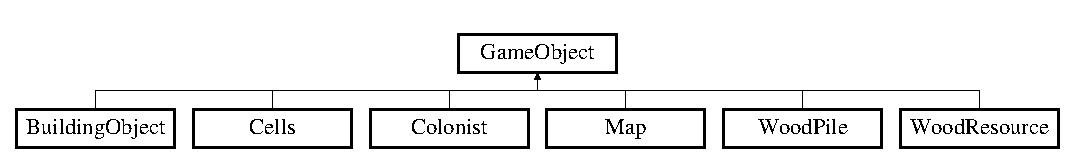
\includegraphics[height=1.761006cm]{class_game_object}
\end{center}
\end{figure}
\subsection*{Public Member Functions}
\begin{DoxyCompactItemize}
\item 
virtual void \mbox{\hyperlink{class_game_object_a3af5a7b470e09f13a1422439fc6a9ba8}{m\+\_\+\+Update}} ()=0
\item 
virtual void \mbox{\hyperlink{class_game_object_a184ac59fd5167c55a54b50894e5b6721}{m\+\_\+\+Draw\+Game\+Object}} (sf\+::\+Render\+Window \&window)=0
\item 
virtual void \mbox{\hyperlink{class_game_object_af1a0662ca445d878b163c4648f90259c}{m\+\_\+\+Draw\+Filter}} (sf\+::\+Vector2f top\+Left, sf\+::\+Vector2f bottom\+Right)=0
\item 
virtual void \mbox{\hyperlink{class_game_object_ad1f8ea8eb3673b1af8215bf92cdc0df8}{m\+\_\+\+Set\+Object\+Pos}} (float x, float y)=0
\item 
sf\+::\+Vector2f \mbox{\hyperlink{class_game_object_a3ab12f6c943557e7ab6d9f56f4bb4953}{m\+\_\+\+Get\+Object\+Pos}} ()
\end{DoxyCompactItemize}
\subsection*{Protected Attributes}
\begin{DoxyCompactItemize}
\item 
sf\+::\+Vector2f \mbox{\hyperlink{class_game_object_a8d07ca1aef7f289bb8cbdca91c0f3f82}{m\+\_\+\+Game\+Object\+Pos}}
\item 
\mbox{\hyperlink{_game_object_8h_a9609a9a703d8f2cd54b9490ab5375b1f}{draw\+Item}} \mbox{\hyperlink{class_game_object_a2e0b93a38fc8523e1be5790e647e6be3}{m\+\_\+\+Draw\+Item}}
\end{DoxyCompactItemize}


\subsection{Member Function Documentation}
\mbox{\Hypertarget{class_game_object_af1a0662ca445d878b163c4648f90259c}\label{class_game_object_af1a0662ca445d878b163c4648f90259c}} 
\index{Game\+Object@{Game\+Object}!m\+\_\+\+Draw\+Filter@{m\+\_\+\+Draw\+Filter}}
\index{m\+\_\+\+Draw\+Filter@{m\+\_\+\+Draw\+Filter}!Game\+Object@{Game\+Object}}
\subsubsection{\texorpdfstring{m\+\_\+\+Draw\+Filter()}{m\_DrawFilter()}}
{\footnotesize\ttfamily virtual void Game\+Object\+::m\+\_\+\+Draw\+Filter (\begin{DoxyParamCaption}\item[{sf\+::\+Vector2f}]{top\+Left,  }\item[{sf\+::\+Vector2f}]{bottom\+Right }\end{DoxyParamCaption})\hspace{0.3cm}{\ttfamily [pure virtual]}}



Implemented in \mbox{\hyperlink{class_cells_a9c7eea82ba5ab8a840bbdcc0be25200f}{Cells}}, \mbox{\hyperlink{class_colonist_a77963df06b74b1235341e235ba7b320e}{Colonist}}, \mbox{\hyperlink{class_map_a47f69ae4c316d2efe45bd8a066e982c9}{Map}}, \mbox{\hyperlink{class_building_object_a05e1b08fb5edd953b00e6deade8bad9d}{Building\+Object}}, \mbox{\hyperlink{class_wood_resource_a08e9ac9417b6337b4fe8afcb97783acf}{Wood\+Resource}}, and \mbox{\hyperlink{class_wood_pile_a4434a4c1251a6719b76825a7546ca04c}{Wood\+Pile}}.

\mbox{\Hypertarget{class_game_object_a184ac59fd5167c55a54b50894e5b6721}\label{class_game_object_a184ac59fd5167c55a54b50894e5b6721}} 
\index{Game\+Object@{Game\+Object}!m\+\_\+\+Draw\+Game\+Object@{m\+\_\+\+Draw\+Game\+Object}}
\index{m\+\_\+\+Draw\+Game\+Object@{m\+\_\+\+Draw\+Game\+Object}!Game\+Object@{Game\+Object}}
\subsubsection{\texorpdfstring{m\+\_\+\+Draw\+Game\+Object()}{m\_DrawGameObject()}}
{\footnotesize\ttfamily virtual void Game\+Object\+::m\+\_\+\+Draw\+Game\+Object (\begin{DoxyParamCaption}\item[{sf\+::\+Render\+Window \&}]{window }\end{DoxyParamCaption})\hspace{0.3cm}{\ttfamily [pure virtual]}}



Implemented in \mbox{\hyperlink{class_cells_a09ab1aeac5c986cc28f52754fafd8c66}{Cells}}, \mbox{\hyperlink{class_colonist_ae7d7c74ff639334e6992142c01dd8f6f}{Colonist}}, \mbox{\hyperlink{class_map_aa65945c61f28808b549a264a3b87219e}{Map}}, \mbox{\hyperlink{class_building_object_a7e343d32ad1f6aaed5ed484b2aabe700}{Building\+Object}}, \mbox{\hyperlink{class_wood_resource_a8f2336619be4467ba0eba87ded7b7474}{Wood\+Resource}}, and \mbox{\hyperlink{class_wood_pile_aacdd6153eacdeaf06cddf83cca50da03}{Wood\+Pile}}.

\mbox{\Hypertarget{class_game_object_a3ab12f6c943557e7ab6d9f56f4bb4953}\label{class_game_object_a3ab12f6c943557e7ab6d9f56f4bb4953}} 
\index{Game\+Object@{Game\+Object}!m\+\_\+\+Get\+Object\+Pos@{m\+\_\+\+Get\+Object\+Pos}}
\index{m\+\_\+\+Get\+Object\+Pos@{m\+\_\+\+Get\+Object\+Pos}!Game\+Object@{Game\+Object}}
\subsubsection{\texorpdfstring{m\+\_\+\+Get\+Object\+Pos()}{m\_GetObjectPos()}}
{\footnotesize\ttfamily sf\+::\+Vector2f Game\+Object\+::m\+\_\+\+Get\+Object\+Pos (\begin{DoxyParamCaption}{ }\end{DoxyParamCaption})}

\mbox{\Hypertarget{class_game_object_ad1f8ea8eb3673b1af8215bf92cdc0df8}\label{class_game_object_ad1f8ea8eb3673b1af8215bf92cdc0df8}} 
\index{Game\+Object@{Game\+Object}!m\+\_\+\+Set\+Object\+Pos@{m\+\_\+\+Set\+Object\+Pos}}
\index{m\+\_\+\+Set\+Object\+Pos@{m\+\_\+\+Set\+Object\+Pos}!Game\+Object@{Game\+Object}}
\subsubsection{\texorpdfstring{m\+\_\+\+Set\+Object\+Pos()}{m\_SetObjectPos()}}
{\footnotesize\ttfamily virtual void Game\+Object\+::m\+\_\+\+Set\+Object\+Pos (\begin{DoxyParamCaption}\item[{float}]{x,  }\item[{float}]{y }\end{DoxyParamCaption})\hspace{0.3cm}{\ttfamily [pure virtual]}}



Implemented in \mbox{\hyperlink{class_colonist_a4dd53225a89bab611509a4d8fc0c2fb1}{Colonist}}, \mbox{\hyperlink{class_cells_a5d900205d8d5fc3d3b41b664d51994c4}{Cells}}, \mbox{\hyperlink{class_map_aa44fadcea160127a186720c1ff44e533}{Map}}, \mbox{\hyperlink{class_building_object_aa6239662e4277d8e1933f9c8fd487511}{Building\+Object}}, \mbox{\hyperlink{class_wood_resource_afa9f748e3dea5f08c18dd831f04d9287}{Wood\+Resource}}, and \mbox{\hyperlink{class_wood_pile_a8faa580584607dea772076b7d856daf8}{Wood\+Pile}}.

\mbox{\Hypertarget{class_game_object_a3af5a7b470e09f13a1422439fc6a9ba8}\label{class_game_object_a3af5a7b470e09f13a1422439fc6a9ba8}} 
\index{Game\+Object@{Game\+Object}!m\+\_\+\+Update@{m\+\_\+\+Update}}
\index{m\+\_\+\+Update@{m\+\_\+\+Update}!Game\+Object@{Game\+Object}}
\subsubsection{\texorpdfstring{m\+\_\+\+Update()}{m\_Update()}}
{\footnotesize\ttfamily virtual void Game\+Object\+::m\+\_\+\+Update (\begin{DoxyParamCaption}{ }\end{DoxyParamCaption})\hspace{0.3cm}{\ttfamily [pure virtual]}}



Implemented in \mbox{\hyperlink{class_cells_a524d410412de7030016b99a4d8b0c1cc}{Cells}}, \mbox{\hyperlink{class_colonist_ad51f196ece25322b1ab2a229875ac490}{Colonist}}, \mbox{\hyperlink{class_building_object_a35fc31e0f1c9a1323b7dfedc527fccff}{Building\+Object}}, \mbox{\hyperlink{class_wood_resource_a8ba1b597aacbdd74be37d0ab18d95008}{Wood\+Resource}}, \mbox{\hyperlink{class_map_a50d9a80e029be4f056b8c5d73791b6c4}{Map}}, and \mbox{\hyperlink{class_wood_pile_a008e8dc7b168ab4e0bcc946c240d0a32}{Wood\+Pile}}.



\subsection{Member Data Documentation}
\mbox{\Hypertarget{class_game_object_a2e0b93a38fc8523e1be5790e647e6be3}\label{class_game_object_a2e0b93a38fc8523e1be5790e647e6be3}} 
\index{Game\+Object@{Game\+Object}!m\+\_\+\+Draw\+Item@{m\+\_\+\+Draw\+Item}}
\index{m\+\_\+\+Draw\+Item@{m\+\_\+\+Draw\+Item}!Game\+Object@{Game\+Object}}
\subsubsection{\texorpdfstring{m\+\_\+\+Draw\+Item}{m\_DrawItem}}
{\footnotesize\ttfamily \mbox{\hyperlink{_game_object_8h_a9609a9a703d8f2cd54b9490ab5375b1f}{draw\+Item}} Game\+Object\+::m\+\_\+\+Draw\+Item\hspace{0.3cm}{\ttfamily [protected]}}

\mbox{\Hypertarget{class_game_object_a8d07ca1aef7f289bb8cbdca91c0f3f82}\label{class_game_object_a8d07ca1aef7f289bb8cbdca91c0f3f82}} 
\index{Game\+Object@{Game\+Object}!m\+\_\+\+Game\+Object\+Pos@{m\+\_\+\+Game\+Object\+Pos}}
\index{m\+\_\+\+Game\+Object\+Pos@{m\+\_\+\+Game\+Object\+Pos}!Game\+Object@{Game\+Object}}
\subsubsection{\texorpdfstring{m\+\_\+\+Game\+Object\+Pos}{m\_GameObjectPos}}
{\footnotesize\ttfamily sf\+::\+Vector2f Game\+Object\+::m\+\_\+\+Game\+Object\+Pos\hspace{0.3cm}{\ttfamily [protected]}}



The documentation for this class was generated from the following file\+:\begin{DoxyCompactItemize}
\item 
inc/\mbox{\hyperlink{_game_object_8h}{Game\+Object.\+h}}\end{DoxyCompactItemize}

\hypertarget{class_grid}{}\section{Grid Class Reference}
\label{class_grid}\index{Grid@{Grid}}


{\ttfamily \#include $<$Grid.\+h$>$}

Inheritance diagram for Grid\+:\begin{figure}[H]
\begin{center}
\leavevmode
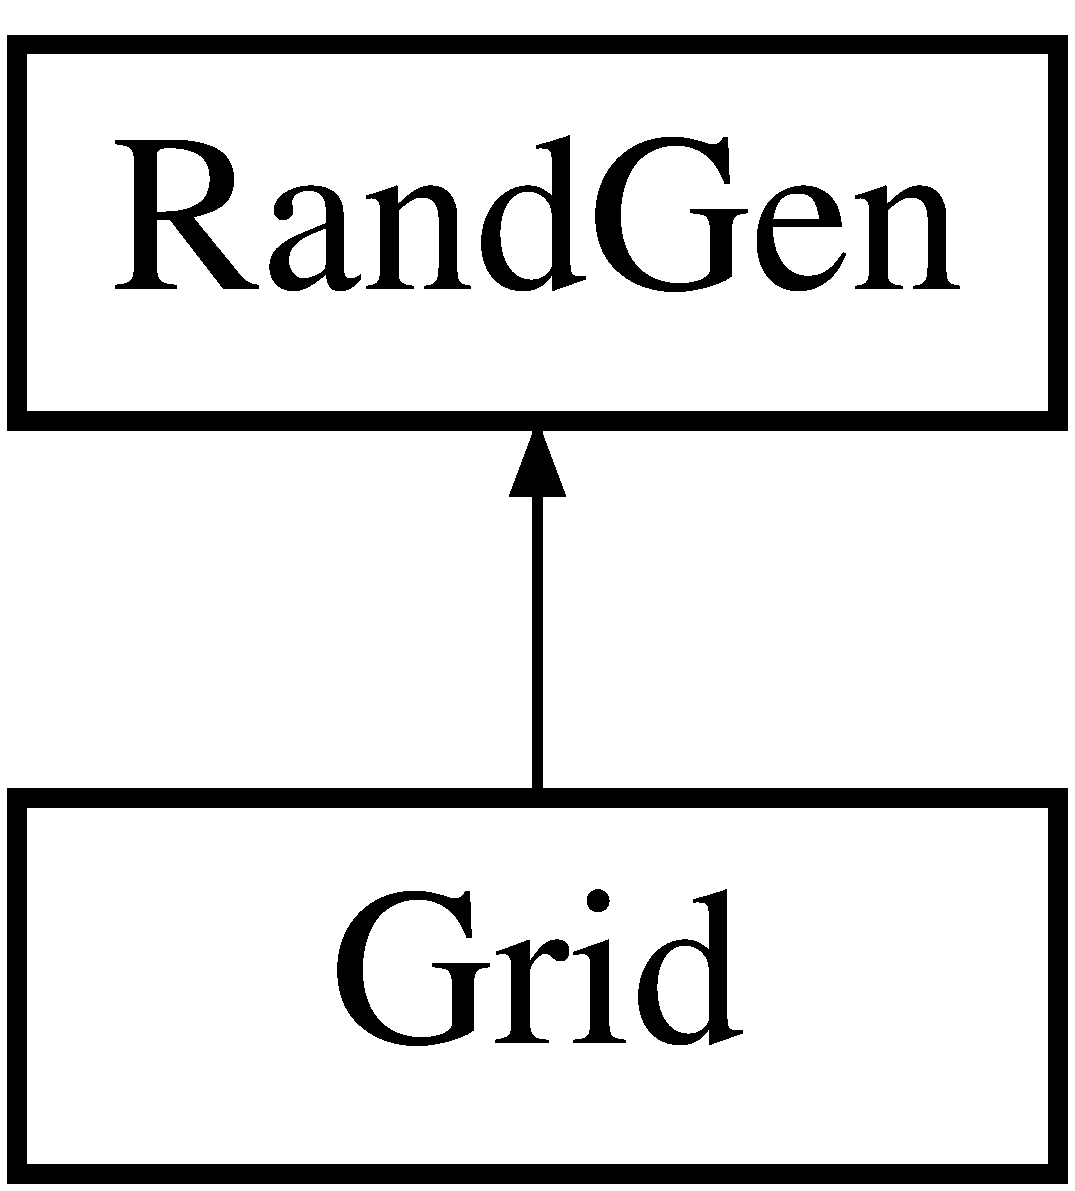
\includegraphics[height=2.000000cm]{class_grid}
\end{center}
\end{figure}
\subsection*{Public Member Functions}
\begin{DoxyCompactItemize}
\item 
\mbox{\hyperlink{class_grid_a4ac9ff4f63552b4c61ff90fcb35ad66c}{Grid}} ()
\item 
\mbox{\hyperlink{class_grid_a3661d0a7f998caaaf8627d7a67072116}{$\sim$\+Grid}} ()
\item 
void \mbox{\hyperlink{class_grid_a0868e8a5ebf55a8746637300bc7aa68b}{m\+\_\+\+Create\+Grid}} (unsigned int rows, unsigned int columns, unsigned int layers, sf\+::\+Rectangle\+Shape grid\+Location)
\item 
void \mbox{\hyperlink{class_grid_a0aa6c9b7aa63b06925be47ef0eeda314}{m\+\_\+\+Assign\+Neighbours}} ()
\item 
void \mbox{\hyperlink{class_grid_ac97a49844ee993f6afe89ae1518e5f44}{m\+\_\+\+Create\+Lake}} (int cellX, int cellY, int layer, int number\+Of\+Iterations)
\item 
void \mbox{\hyperlink{class_grid_a5e87248bee8835c61b1977407f5ef034}{m\+\_\+\+Create\+River}} (std\+::deque$<$ \mbox{\hyperlink{class_cells}{Cells}} $\ast$$>$ river\+Path, int river\+Width, int layer)
\item 
void \mbox{\hyperlink{class_grid_a32c88ba0de0530b6d4c1b0ab2cde31dc}{m\+\_\+\+Create\+Underground\+Water}} (int min\+Layer, int max\+Layer)
\item 
void \mbox{\hyperlink{class_grid_a8d5e70ea3e0fac523d409882b4c3949c}{m\+\_\+\+Create\+Rock}} (int layer)
\item 
void \mbox{\hyperlink{class_grid_a5b15f505b7508caeb457c0b218482164}{m\+\_\+\+Create\+Underground\+Rock}} (int min\+Layer, int max\+Layer)
\item 
void \mbox{\hyperlink{class_grid_a121458c828be458c452e5f6c80c07cc9}{m\+\_\+\+Create\+Upper\+Rock}} (int min\+Layer, int max\+Layer)
\item 
void \mbox{\hyperlink{class_grid_aa0ee683a771225bfdbe07ecd6c4341fb}{m\+\_\+\+Create\+Dirt}} (int layer)
\item 
void \mbox{\hyperlink{class_grid_a315b11046448a05d48d949eb296b593f}{m\+\_\+\+Create\+Underground\+Dirt}} (int min\+Layer, int max\+Layer)
\item 
void \mbox{\hyperlink{class_grid_a66df10e620798fde6b1455d9d49bc60c}{m\+\_\+\+Create\+Sky}} (int min\+Layer, int max\+Layer)
\item 
void \mbox{\hyperlink{class_grid_a86e0025cc46907e1c13658a28aa1439c}{m\+\_\+\+Assign\+Textures}} (std\+::map$<$ std\+::string, sf\+::\+Texture $>$ \&m\+\_\+\+Texture\+Map)
\item 
\mbox{\hyperlink{class_cells}{Cells}} $\ast$ \mbox{\hyperlink{class_grid_a12c587d1708736010999fa4e1e7601e0}{m\+\_\+\+Get\+Cell}} (int layer, int x, int y)
\item 
\mbox{\hyperlink{class_cells}{Cells}} $\ast$ \mbox{\hyperlink{class_grid_a7464f3bbe32feea62b940522e686fa3b}{m\+\_\+\+Get\+Random\+Dirt\+Cell}} (int layer)
\item 
\mbox{\hyperlink{class_cells}{Cells}} $\ast$ \mbox{\hyperlink{class_grid_ac1e06043497ba5c2b5c7e83d910f90a0}{m\+\_\+\+Convert\+World\+Pos\+To\+Grid\+Pos}} (sf\+::\+Vector2f current\+Pos, unsigned int layer)
\item 
unsigned int \mbox{\hyperlink{class_grid_a4a783e0c327cf99e7e831e511ce07847}{m\+\_\+\+Get\+Number\+Of\+Layers}} ()
\item 
unsigned int \mbox{\hyperlink{class_grid_aa14c1738133d778e8b2484afda051117}{m\+\_\+\+Get\+Number\+Of\+Rows}} ()
\item 
unsigned int \mbox{\hyperlink{class_grid_af11836b4b3d9fb8d5fe9da6bfae9a951}{m\+\_\+\+Get\+Number\+Of\+Columns}} ()
\item 
void \mbox{\hyperlink{class_grid_a7ffff576d982720579377833e17fd63f}{m\+\_\+\+Draw\+Grid}} (sf\+::\+Render\+Window \&window, unsigned int layer)
\item 
void \mbox{\hyperlink{class_grid_a07d1b32ae5330664bfd15466cffb1118}{m\+\_\+\+Check\+Items\+For\+Render}} (sf\+::\+Vector2f top\+Left, sf\+::\+Vector2f bottom\+Right, unsigned int layer)
\end{DoxyCompactItemize}


\subsection{Constructor \& Destructor Documentation}
\mbox{\Hypertarget{class_grid_a4ac9ff4f63552b4c61ff90fcb35ad66c}\label{class_grid_a4ac9ff4f63552b4c61ff90fcb35ad66c}} 
\index{Grid@{Grid}!Grid@{Grid}}
\index{Grid@{Grid}!Grid@{Grid}}
\subsubsection{\texorpdfstring{Grid()}{Grid()}}
{\footnotesize\ttfamily Grid\+::\+Grid (\begin{DoxyParamCaption}{ }\end{DoxyParamCaption})}

\mbox{\Hypertarget{class_grid_a3661d0a7f998caaaf8627d7a67072116}\label{class_grid_a3661d0a7f998caaaf8627d7a67072116}} 
\index{Grid@{Grid}!````~Grid@{$\sim$\+Grid}}
\index{````~Grid@{$\sim$\+Grid}!Grid@{Grid}}
\subsubsection{\texorpdfstring{$\sim$\+Grid()}{~Grid()}}
{\footnotesize\ttfamily Grid\+::$\sim$\+Grid (\begin{DoxyParamCaption}{ }\end{DoxyParamCaption})}



\subsection{Member Function Documentation}
\mbox{\Hypertarget{class_grid_a0aa6c9b7aa63b06925be47ef0eeda314}\label{class_grid_a0aa6c9b7aa63b06925be47ef0eeda314}} 
\index{Grid@{Grid}!m\+\_\+\+Assign\+Neighbours@{m\+\_\+\+Assign\+Neighbours}}
\index{m\+\_\+\+Assign\+Neighbours@{m\+\_\+\+Assign\+Neighbours}!Grid@{Grid}}
\subsubsection{\texorpdfstring{m\+\_\+\+Assign\+Neighbours()}{m\_AssignNeighbours()}}
{\footnotesize\ttfamily void Grid\+::m\+\_\+\+Assign\+Neighbours (\begin{DoxyParamCaption}{ }\end{DoxyParamCaption})}

\mbox{\Hypertarget{class_grid_a86e0025cc46907e1c13658a28aa1439c}\label{class_grid_a86e0025cc46907e1c13658a28aa1439c}} 
\index{Grid@{Grid}!m\+\_\+\+Assign\+Textures@{m\+\_\+\+Assign\+Textures}}
\index{m\+\_\+\+Assign\+Textures@{m\+\_\+\+Assign\+Textures}!Grid@{Grid}}
\subsubsection{\texorpdfstring{m\+\_\+\+Assign\+Textures()}{m\_AssignTextures()}}
{\footnotesize\ttfamily void Grid\+::m\+\_\+\+Assign\+Textures (\begin{DoxyParamCaption}\item[{std\+::map$<$ std\+::string, sf\+::\+Texture $>$ \&}]{m\+\_\+\+Texture\+Map }\end{DoxyParamCaption})}

\mbox{\Hypertarget{class_grid_a07d1b32ae5330664bfd15466cffb1118}\label{class_grid_a07d1b32ae5330664bfd15466cffb1118}} 
\index{Grid@{Grid}!m\+\_\+\+Check\+Items\+For\+Render@{m\+\_\+\+Check\+Items\+For\+Render}}
\index{m\+\_\+\+Check\+Items\+For\+Render@{m\+\_\+\+Check\+Items\+For\+Render}!Grid@{Grid}}
\subsubsection{\texorpdfstring{m\+\_\+\+Check\+Items\+For\+Render()}{m\_CheckItemsForRender()}}
{\footnotesize\ttfamily void Grid\+::m\+\_\+\+Check\+Items\+For\+Render (\begin{DoxyParamCaption}\item[{sf\+::\+Vector2f}]{top\+Left,  }\item[{sf\+::\+Vector2f}]{bottom\+Right,  }\item[{unsigned int}]{layer }\end{DoxyParamCaption})}

\mbox{\Hypertarget{class_grid_ac1e06043497ba5c2b5c7e83d910f90a0}\label{class_grid_ac1e06043497ba5c2b5c7e83d910f90a0}} 
\index{Grid@{Grid}!m\+\_\+\+Convert\+World\+Pos\+To\+Grid\+Pos@{m\+\_\+\+Convert\+World\+Pos\+To\+Grid\+Pos}}
\index{m\+\_\+\+Convert\+World\+Pos\+To\+Grid\+Pos@{m\+\_\+\+Convert\+World\+Pos\+To\+Grid\+Pos}!Grid@{Grid}}
\subsubsection{\texorpdfstring{m\+\_\+\+Convert\+World\+Pos\+To\+Grid\+Pos()}{m\_ConvertWorldPosToGridPos()}}
{\footnotesize\ttfamily \mbox{\hyperlink{class_cells}{Cells}}$\ast$ Grid\+::m\+\_\+\+Convert\+World\+Pos\+To\+Grid\+Pos (\begin{DoxyParamCaption}\item[{sf\+::\+Vector2f}]{current\+Pos,  }\item[{unsigned int}]{layer }\end{DoxyParamCaption})}

\mbox{\Hypertarget{class_grid_aa0ee683a771225bfdbe07ecd6c4341fb}\label{class_grid_aa0ee683a771225bfdbe07ecd6c4341fb}} 
\index{Grid@{Grid}!m\+\_\+\+Create\+Dirt@{m\+\_\+\+Create\+Dirt}}
\index{m\+\_\+\+Create\+Dirt@{m\+\_\+\+Create\+Dirt}!Grid@{Grid}}
\subsubsection{\texorpdfstring{m\+\_\+\+Create\+Dirt()}{m\_CreateDirt()}}
{\footnotesize\ttfamily void Grid\+::m\+\_\+\+Create\+Dirt (\begin{DoxyParamCaption}\item[{int}]{layer }\end{DoxyParamCaption})}

\mbox{\Hypertarget{class_grid_a0868e8a5ebf55a8746637300bc7aa68b}\label{class_grid_a0868e8a5ebf55a8746637300bc7aa68b}} 
\index{Grid@{Grid}!m\+\_\+\+Create\+Grid@{m\+\_\+\+Create\+Grid}}
\index{m\+\_\+\+Create\+Grid@{m\+\_\+\+Create\+Grid}!Grid@{Grid}}
\subsubsection{\texorpdfstring{m\+\_\+\+Create\+Grid()}{m\_CreateGrid()}}
{\footnotesize\ttfamily void Grid\+::m\+\_\+\+Create\+Grid (\begin{DoxyParamCaption}\item[{unsigned int}]{rows,  }\item[{unsigned int}]{columns,  }\item[{unsigned int}]{layers,  }\item[{sf\+::\+Rectangle\+Shape}]{grid\+Location }\end{DoxyParamCaption})}

\mbox{\Hypertarget{class_grid_ac97a49844ee993f6afe89ae1518e5f44}\label{class_grid_ac97a49844ee993f6afe89ae1518e5f44}} 
\index{Grid@{Grid}!m\+\_\+\+Create\+Lake@{m\+\_\+\+Create\+Lake}}
\index{m\+\_\+\+Create\+Lake@{m\+\_\+\+Create\+Lake}!Grid@{Grid}}
\subsubsection{\texorpdfstring{m\+\_\+\+Create\+Lake()}{m\_CreateLake()}}
{\footnotesize\ttfamily void Grid\+::m\+\_\+\+Create\+Lake (\begin{DoxyParamCaption}\item[{int}]{cellX,  }\item[{int}]{cellY,  }\item[{int}]{layer,  }\item[{int}]{number\+Of\+Iterations }\end{DoxyParamCaption})}

\mbox{\Hypertarget{class_grid_a5e87248bee8835c61b1977407f5ef034}\label{class_grid_a5e87248bee8835c61b1977407f5ef034}} 
\index{Grid@{Grid}!m\+\_\+\+Create\+River@{m\+\_\+\+Create\+River}}
\index{m\+\_\+\+Create\+River@{m\+\_\+\+Create\+River}!Grid@{Grid}}
\subsubsection{\texorpdfstring{m\+\_\+\+Create\+River()}{m\_CreateRiver()}}
{\footnotesize\ttfamily void Grid\+::m\+\_\+\+Create\+River (\begin{DoxyParamCaption}\item[{std\+::deque$<$ \mbox{\hyperlink{class_cells}{Cells}} $\ast$$>$}]{river\+Path,  }\item[{int}]{river\+Width,  }\item[{int}]{layer }\end{DoxyParamCaption})}

\mbox{\Hypertarget{class_grid_a8d5e70ea3e0fac523d409882b4c3949c}\label{class_grid_a8d5e70ea3e0fac523d409882b4c3949c}} 
\index{Grid@{Grid}!m\+\_\+\+Create\+Rock@{m\+\_\+\+Create\+Rock}}
\index{m\+\_\+\+Create\+Rock@{m\+\_\+\+Create\+Rock}!Grid@{Grid}}
\subsubsection{\texorpdfstring{m\+\_\+\+Create\+Rock()}{m\_CreateRock()}}
{\footnotesize\ttfamily void Grid\+::m\+\_\+\+Create\+Rock (\begin{DoxyParamCaption}\item[{int}]{layer }\end{DoxyParamCaption})}

\mbox{\Hypertarget{class_grid_a66df10e620798fde6b1455d9d49bc60c}\label{class_grid_a66df10e620798fde6b1455d9d49bc60c}} 
\index{Grid@{Grid}!m\+\_\+\+Create\+Sky@{m\+\_\+\+Create\+Sky}}
\index{m\+\_\+\+Create\+Sky@{m\+\_\+\+Create\+Sky}!Grid@{Grid}}
\subsubsection{\texorpdfstring{m\+\_\+\+Create\+Sky()}{m\_CreateSky()}}
{\footnotesize\ttfamily void Grid\+::m\+\_\+\+Create\+Sky (\begin{DoxyParamCaption}\item[{int}]{min\+Layer,  }\item[{int}]{max\+Layer }\end{DoxyParamCaption})}

\mbox{\Hypertarget{class_grid_a315b11046448a05d48d949eb296b593f}\label{class_grid_a315b11046448a05d48d949eb296b593f}} 
\index{Grid@{Grid}!m\+\_\+\+Create\+Underground\+Dirt@{m\+\_\+\+Create\+Underground\+Dirt}}
\index{m\+\_\+\+Create\+Underground\+Dirt@{m\+\_\+\+Create\+Underground\+Dirt}!Grid@{Grid}}
\subsubsection{\texorpdfstring{m\+\_\+\+Create\+Underground\+Dirt()}{m\_CreateUndergroundDirt()}}
{\footnotesize\ttfamily void Grid\+::m\+\_\+\+Create\+Underground\+Dirt (\begin{DoxyParamCaption}\item[{int}]{min\+Layer,  }\item[{int}]{max\+Layer }\end{DoxyParamCaption})}

\mbox{\Hypertarget{class_grid_a5b15f505b7508caeb457c0b218482164}\label{class_grid_a5b15f505b7508caeb457c0b218482164}} 
\index{Grid@{Grid}!m\+\_\+\+Create\+Underground\+Rock@{m\+\_\+\+Create\+Underground\+Rock}}
\index{m\+\_\+\+Create\+Underground\+Rock@{m\+\_\+\+Create\+Underground\+Rock}!Grid@{Grid}}
\subsubsection{\texorpdfstring{m\+\_\+\+Create\+Underground\+Rock()}{m\_CreateUndergroundRock()}}
{\footnotesize\ttfamily void Grid\+::m\+\_\+\+Create\+Underground\+Rock (\begin{DoxyParamCaption}\item[{int}]{min\+Layer,  }\item[{int}]{max\+Layer }\end{DoxyParamCaption})}

\mbox{\Hypertarget{class_grid_a32c88ba0de0530b6d4c1b0ab2cde31dc}\label{class_grid_a32c88ba0de0530b6d4c1b0ab2cde31dc}} 
\index{Grid@{Grid}!m\+\_\+\+Create\+Underground\+Water@{m\+\_\+\+Create\+Underground\+Water}}
\index{m\+\_\+\+Create\+Underground\+Water@{m\+\_\+\+Create\+Underground\+Water}!Grid@{Grid}}
\subsubsection{\texorpdfstring{m\+\_\+\+Create\+Underground\+Water()}{m\_CreateUndergroundWater()}}
{\footnotesize\ttfamily void Grid\+::m\+\_\+\+Create\+Underground\+Water (\begin{DoxyParamCaption}\item[{int}]{min\+Layer,  }\item[{int}]{max\+Layer }\end{DoxyParamCaption})}

\mbox{\Hypertarget{class_grid_a121458c828be458c452e5f6c80c07cc9}\label{class_grid_a121458c828be458c452e5f6c80c07cc9}} 
\index{Grid@{Grid}!m\+\_\+\+Create\+Upper\+Rock@{m\+\_\+\+Create\+Upper\+Rock}}
\index{m\+\_\+\+Create\+Upper\+Rock@{m\+\_\+\+Create\+Upper\+Rock}!Grid@{Grid}}
\subsubsection{\texorpdfstring{m\+\_\+\+Create\+Upper\+Rock()}{m\_CreateUpperRock()}}
{\footnotesize\ttfamily void Grid\+::m\+\_\+\+Create\+Upper\+Rock (\begin{DoxyParamCaption}\item[{int}]{min\+Layer,  }\item[{int}]{max\+Layer }\end{DoxyParamCaption})}

\mbox{\Hypertarget{class_grid_a7ffff576d982720579377833e17fd63f}\label{class_grid_a7ffff576d982720579377833e17fd63f}} 
\index{Grid@{Grid}!m\+\_\+\+Draw\+Grid@{m\+\_\+\+Draw\+Grid}}
\index{m\+\_\+\+Draw\+Grid@{m\+\_\+\+Draw\+Grid}!Grid@{Grid}}
\subsubsection{\texorpdfstring{m\+\_\+\+Draw\+Grid()}{m\_DrawGrid()}}
{\footnotesize\ttfamily void Grid\+::m\+\_\+\+Draw\+Grid (\begin{DoxyParamCaption}\item[{sf\+::\+Render\+Window \&}]{window,  }\item[{unsigned int}]{layer }\end{DoxyParamCaption})}

\mbox{\Hypertarget{class_grid_a12c587d1708736010999fa4e1e7601e0}\label{class_grid_a12c587d1708736010999fa4e1e7601e0}} 
\index{Grid@{Grid}!m\+\_\+\+Get\+Cell@{m\+\_\+\+Get\+Cell}}
\index{m\+\_\+\+Get\+Cell@{m\+\_\+\+Get\+Cell}!Grid@{Grid}}
\subsubsection{\texorpdfstring{m\+\_\+\+Get\+Cell()}{m\_GetCell()}}
{\footnotesize\ttfamily \mbox{\hyperlink{class_cells}{Cells}}$\ast$ Grid\+::m\+\_\+\+Get\+Cell (\begin{DoxyParamCaption}\item[{int}]{layer,  }\item[{int}]{x,  }\item[{int}]{y }\end{DoxyParamCaption})}

\mbox{\Hypertarget{class_grid_af11836b4b3d9fb8d5fe9da6bfae9a951}\label{class_grid_af11836b4b3d9fb8d5fe9da6bfae9a951}} 
\index{Grid@{Grid}!m\+\_\+\+Get\+Number\+Of\+Columns@{m\+\_\+\+Get\+Number\+Of\+Columns}}
\index{m\+\_\+\+Get\+Number\+Of\+Columns@{m\+\_\+\+Get\+Number\+Of\+Columns}!Grid@{Grid}}
\subsubsection{\texorpdfstring{m\+\_\+\+Get\+Number\+Of\+Columns()}{m\_GetNumberOfColumns()}}
{\footnotesize\ttfamily unsigned int Grid\+::m\+\_\+\+Get\+Number\+Of\+Columns (\begin{DoxyParamCaption}{ }\end{DoxyParamCaption})}

\mbox{\Hypertarget{class_grid_a4a783e0c327cf99e7e831e511ce07847}\label{class_grid_a4a783e0c327cf99e7e831e511ce07847}} 
\index{Grid@{Grid}!m\+\_\+\+Get\+Number\+Of\+Layers@{m\+\_\+\+Get\+Number\+Of\+Layers}}
\index{m\+\_\+\+Get\+Number\+Of\+Layers@{m\+\_\+\+Get\+Number\+Of\+Layers}!Grid@{Grid}}
\subsubsection{\texorpdfstring{m\+\_\+\+Get\+Number\+Of\+Layers()}{m\_GetNumberOfLayers()}}
{\footnotesize\ttfamily unsigned int Grid\+::m\+\_\+\+Get\+Number\+Of\+Layers (\begin{DoxyParamCaption}{ }\end{DoxyParamCaption})}

\mbox{\Hypertarget{class_grid_aa14c1738133d778e8b2484afda051117}\label{class_grid_aa14c1738133d778e8b2484afda051117}} 
\index{Grid@{Grid}!m\+\_\+\+Get\+Number\+Of\+Rows@{m\+\_\+\+Get\+Number\+Of\+Rows}}
\index{m\+\_\+\+Get\+Number\+Of\+Rows@{m\+\_\+\+Get\+Number\+Of\+Rows}!Grid@{Grid}}
\subsubsection{\texorpdfstring{m\+\_\+\+Get\+Number\+Of\+Rows()}{m\_GetNumberOfRows()}}
{\footnotesize\ttfamily unsigned int Grid\+::m\+\_\+\+Get\+Number\+Of\+Rows (\begin{DoxyParamCaption}{ }\end{DoxyParamCaption})}

\mbox{\Hypertarget{class_grid_a7464f3bbe32feea62b940522e686fa3b}\label{class_grid_a7464f3bbe32feea62b940522e686fa3b}} 
\index{Grid@{Grid}!m\+\_\+\+Get\+Random\+Dirt\+Cell@{m\+\_\+\+Get\+Random\+Dirt\+Cell}}
\index{m\+\_\+\+Get\+Random\+Dirt\+Cell@{m\+\_\+\+Get\+Random\+Dirt\+Cell}!Grid@{Grid}}
\subsubsection{\texorpdfstring{m\+\_\+\+Get\+Random\+Dirt\+Cell()}{m\_GetRandomDirtCell()}}
{\footnotesize\ttfamily \mbox{\hyperlink{class_cells}{Cells}}$\ast$ Grid\+::m\+\_\+\+Get\+Random\+Dirt\+Cell (\begin{DoxyParamCaption}\item[{int}]{layer }\end{DoxyParamCaption})}



The documentation for this class was generated from the following file\+:\begin{DoxyCompactItemize}
\item 
inc/\mbox{\hyperlink{_grid_8h}{Grid.\+h}}\end{DoxyCompactItemize}

\hypertarget{structgrid_pos}{}\section{grid\+Pos Struct Reference}
\label{structgrid_pos}\index{grid\+Pos@{grid\+Pos}}


{\ttfamily \#include $<$Cells.\+h$>$}

\subsection*{Public Attributes}
\begin{DoxyCompactItemize}
\item 
float \mbox{\hyperlink{structgrid_pos_a582a1c50bb78a8460a4820ed010e60e4}{x}}
\item 
float \mbox{\hyperlink{structgrid_pos_a3e6999820e3185735de6d91e3c01da22}{y}}
\end{DoxyCompactItemize}


\subsection{Member Data Documentation}
\mbox{\Hypertarget{structgrid_pos_a582a1c50bb78a8460a4820ed010e60e4}\label{structgrid_pos_a582a1c50bb78a8460a4820ed010e60e4}} 
\index{grid\+Pos@{grid\+Pos}!x@{x}}
\index{x@{x}!grid\+Pos@{grid\+Pos}}
\subsubsection{\texorpdfstring{x}{x}}
{\footnotesize\ttfamily float grid\+Pos\+::x}

\mbox{\Hypertarget{structgrid_pos_a3e6999820e3185735de6d91e3c01da22}\label{structgrid_pos_a3e6999820e3185735de6d91e3c01da22}} 
\index{grid\+Pos@{grid\+Pos}!y@{y}}
\index{y@{y}!grid\+Pos@{grid\+Pos}}
\subsubsection{\texorpdfstring{y}{y}}
{\footnotesize\ttfamily float grid\+Pos\+::y}

The x and y coordinates for \mbox{\hyperlink{class_this}{This}} cell object. 

The documentation for this struct was generated from the following file\+:\begin{DoxyCompactItemize}
\item 
inc/\mbox{\hyperlink{_cells_8h}{Cells.\+h}}\end{DoxyCompactItemize}

\hypertarget{class_info_window}{}\section{Info\+Window Class Reference}
\label{class_info_window}\index{Info\+Window@{Info\+Window}}


{\ttfamily \#include $<$Info\+Window.\+h$>$}

Inheritance diagram for Info\+Window\+:\begin{figure}[H]
\begin{center}
\leavevmode
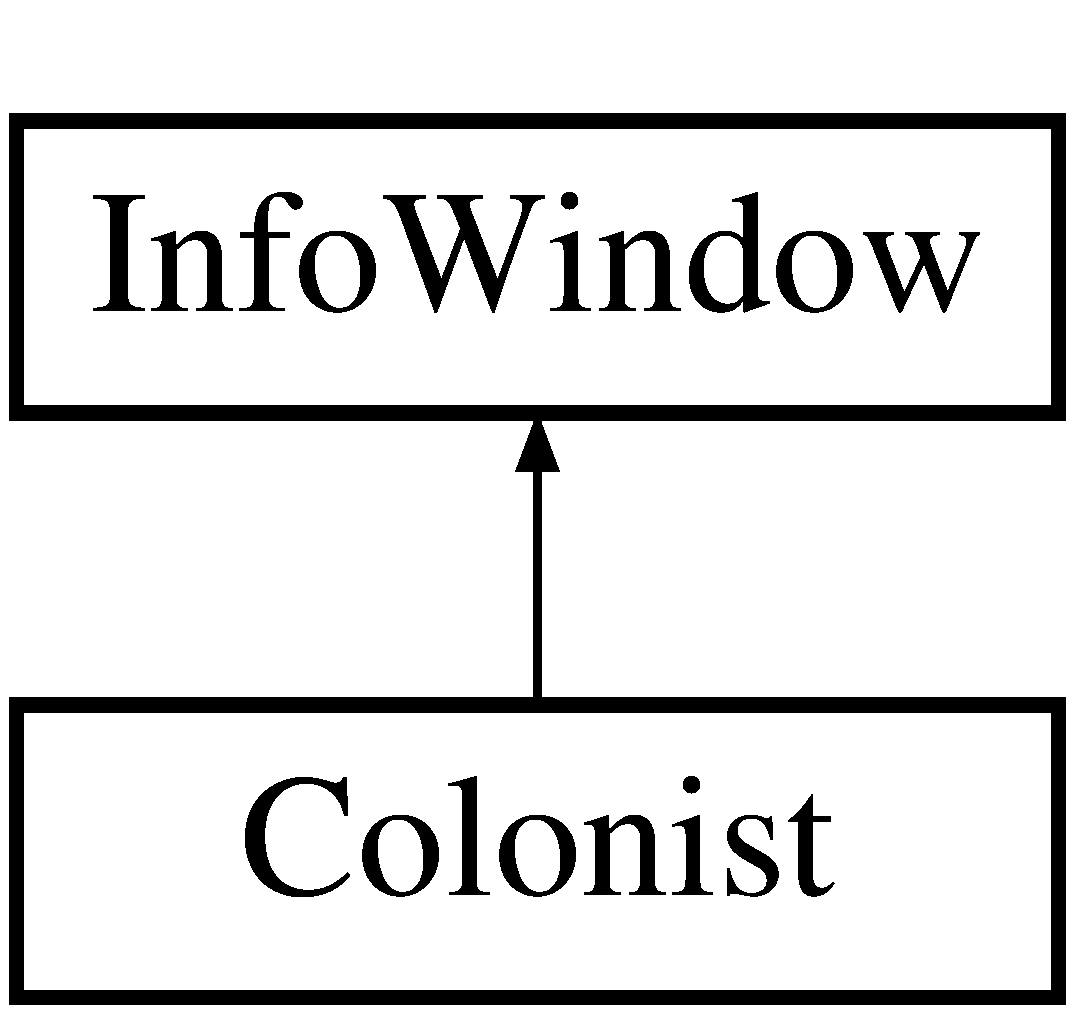
\includegraphics[height=2.000000cm]{class_info_window}
\end{center}
\end{figure}
\subsection*{Public Member Functions}
\begin{DoxyCompactItemize}
\item 
\mbox{\hyperlink{class_info_window_a989cf8d93250fe17f944860b8efdd68d}{Info\+Window}} ()
\item 
\mbox{\hyperlink{class_info_window_a41a3465e5db7d3ac6fa9627ff20fa241}{$\sim$\+Info\+Window}} ()
\item 
void \mbox{\hyperlink{class_info_window_a32e95be032eae3d7954ec4cb149b6be5}{m\+\_\+\+Setup\+Info\+Window}} (sf\+::\+Vector2f dimentions, sf\+::\+Vector2f position)
\item 
void \mbox{\hyperlink{class_info_window_ae53368fe52e5d4d41cc157d3a8582744}{m\+\_\+\+Draw\+Info\+Window}} (sf\+::\+Render\+Window \&window)
\item 
void \mbox{\hyperlink{class_info_window_a1dc630a6d223bdc4bb672bd961f1622e}{m\+\_\+\+Add\+Data\+To\+Map}} (std\+::string data\+Name, int data)
\item 
void \mbox{\hyperlink{class_info_window_a5306b949858741146614d82ba39704d2}{m\+\_\+\+Assign\+Fonts}} (sf\+::\+Font new\+Font)
\item 
void \mbox{\hyperlink{class_info_window_a494f9cbe7a7c89a1073443fbc1a4437f}{m\+\_\+\+Set\+Display}} (bool value)
\item 
void \mbox{\hyperlink{class_info_window_a3b63c075f8c26f96d2569b163a7dfde9}{m\+\_\+\+Update\+Info\+Window}} (sf\+::\+Vector2f View\+Lower\+Bounds, sf\+::\+Vector2f view\+Size)
\end{DoxyCompactItemize}


\subsection{Constructor \& Destructor Documentation}
\mbox{\Hypertarget{class_info_window_a989cf8d93250fe17f944860b8efdd68d}\label{class_info_window_a989cf8d93250fe17f944860b8efdd68d}} 
\index{Info\+Window@{Info\+Window}!Info\+Window@{Info\+Window}}
\index{Info\+Window@{Info\+Window}!Info\+Window@{Info\+Window}}
\subsubsection{\texorpdfstring{Info\+Window()}{InfoWindow()}}
{\footnotesize\ttfamily Info\+Window\+::\+Info\+Window (\begin{DoxyParamCaption}{ }\end{DoxyParamCaption})}

\mbox{\Hypertarget{class_info_window_a41a3465e5db7d3ac6fa9627ff20fa241}\label{class_info_window_a41a3465e5db7d3ac6fa9627ff20fa241}} 
\index{Info\+Window@{Info\+Window}!````~Info\+Window@{$\sim$\+Info\+Window}}
\index{````~Info\+Window@{$\sim$\+Info\+Window}!Info\+Window@{Info\+Window}}
\subsubsection{\texorpdfstring{$\sim$\+Info\+Window()}{~InfoWindow()}}
{\footnotesize\ttfamily Info\+Window\+::$\sim$\+Info\+Window (\begin{DoxyParamCaption}{ }\end{DoxyParamCaption})}



\subsection{Member Function Documentation}
\mbox{\Hypertarget{class_info_window_a1dc630a6d223bdc4bb672bd961f1622e}\label{class_info_window_a1dc630a6d223bdc4bb672bd961f1622e}} 
\index{Info\+Window@{Info\+Window}!m\+\_\+\+Add\+Data\+To\+Map@{m\+\_\+\+Add\+Data\+To\+Map}}
\index{m\+\_\+\+Add\+Data\+To\+Map@{m\+\_\+\+Add\+Data\+To\+Map}!Info\+Window@{Info\+Window}}
\subsubsection{\texorpdfstring{m\+\_\+\+Add\+Data\+To\+Map()}{m\_AddDataToMap()}}
{\footnotesize\ttfamily void Info\+Window\+::m\+\_\+\+Add\+Data\+To\+Map (\begin{DoxyParamCaption}\item[{std\+::string}]{data\+Name,  }\item[{int}]{data }\end{DoxyParamCaption})}

\mbox{\Hypertarget{class_info_window_a5306b949858741146614d82ba39704d2}\label{class_info_window_a5306b949858741146614d82ba39704d2}} 
\index{Info\+Window@{Info\+Window}!m\+\_\+\+Assign\+Fonts@{m\+\_\+\+Assign\+Fonts}}
\index{m\+\_\+\+Assign\+Fonts@{m\+\_\+\+Assign\+Fonts}!Info\+Window@{Info\+Window}}
\subsubsection{\texorpdfstring{m\+\_\+\+Assign\+Fonts()}{m\_AssignFonts()}}
{\footnotesize\ttfamily void Info\+Window\+::m\+\_\+\+Assign\+Fonts (\begin{DoxyParamCaption}\item[{sf\+::\+Font}]{new\+Font }\end{DoxyParamCaption})}

\mbox{\Hypertarget{class_info_window_ae53368fe52e5d4d41cc157d3a8582744}\label{class_info_window_ae53368fe52e5d4d41cc157d3a8582744}} 
\index{Info\+Window@{Info\+Window}!m\+\_\+\+Draw\+Info\+Window@{m\+\_\+\+Draw\+Info\+Window}}
\index{m\+\_\+\+Draw\+Info\+Window@{m\+\_\+\+Draw\+Info\+Window}!Info\+Window@{Info\+Window}}
\subsubsection{\texorpdfstring{m\+\_\+\+Draw\+Info\+Window()}{m\_DrawInfoWindow()}}
{\footnotesize\ttfamily void Info\+Window\+::m\+\_\+\+Draw\+Info\+Window (\begin{DoxyParamCaption}\item[{sf\+::\+Render\+Window \&}]{window }\end{DoxyParamCaption})}

\mbox{\Hypertarget{class_info_window_a494f9cbe7a7c89a1073443fbc1a4437f}\label{class_info_window_a494f9cbe7a7c89a1073443fbc1a4437f}} 
\index{Info\+Window@{Info\+Window}!m\+\_\+\+Set\+Display@{m\+\_\+\+Set\+Display}}
\index{m\+\_\+\+Set\+Display@{m\+\_\+\+Set\+Display}!Info\+Window@{Info\+Window}}
\subsubsection{\texorpdfstring{m\+\_\+\+Set\+Display()}{m\_SetDisplay()}}
{\footnotesize\ttfamily void Info\+Window\+::m\+\_\+\+Set\+Display (\begin{DoxyParamCaption}\item[{bool}]{value }\end{DoxyParamCaption})}

\mbox{\Hypertarget{class_info_window_a32e95be032eae3d7954ec4cb149b6be5}\label{class_info_window_a32e95be032eae3d7954ec4cb149b6be5}} 
\index{Info\+Window@{Info\+Window}!m\+\_\+\+Setup\+Info\+Window@{m\+\_\+\+Setup\+Info\+Window}}
\index{m\+\_\+\+Setup\+Info\+Window@{m\+\_\+\+Setup\+Info\+Window}!Info\+Window@{Info\+Window}}
\subsubsection{\texorpdfstring{m\+\_\+\+Setup\+Info\+Window()}{m\_SetupInfoWindow()}}
{\footnotesize\ttfamily void Info\+Window\+::m\+\_\+\+Setup\+Info\+Window (\begin{DoxyParamCaption}\item[{sf\+::\+Vector2f}]{dimentions,  }\item[{sf\+::\+Vector2f}]{position }\end{DoxyParamCaption})}

\mbox{\Hypertarget{class_info_window_a3b63c075f8c26f96d2569b163a7dfde9}\label{class_info_window_a3b63c075f8c26f96d2569b163a7dfde9}} 
\index{Info\+Window@{Info\+Window}!m\+\_\+\+Update\+Info\+Window@{m\+\_\+\+Update\+Info\+Window}}
\index{m\+\_\+\+Update\+Info\+Window@{m\+\_\+\+Update\+Info\+Window}!Info\+Window@{Info\+Window}}
\subsubsection{\texorpdfstring{m\+\_\+\+Update\+Info\+Window()}{m\_UpdateInfoWindow()}}
{\footnotesize\ttfamily void Info\+Window\+::m\+\_\+\+Update\+Info\+Window (\begin{DoxyParamCaption}\item[{sf\+::\+Vector2f}]{View\+Lower\+Bounds,  }\item[{sf\+::\+Vector2f}]{view\+Size }\end{DoxyParamCaption})}



The documentation for this class was generated from the following file\+:\begin{DoxyCompactItemize}
\item 
inc/\mbox{\hyperlink{_info_window_8h}{Info\+Window.\+h}}\end{DoxyCompactItemize}

\hypertarget{class_map}{}\section{Map Class Reference}
\label{class_map}\index{Map@{Map}}


{\ttfamily \#include $<$Game\+Map.\+h$>$}

Inheritance diagram for Map\+:\begin{figure}[H]
\begin{center}
\leavevmode
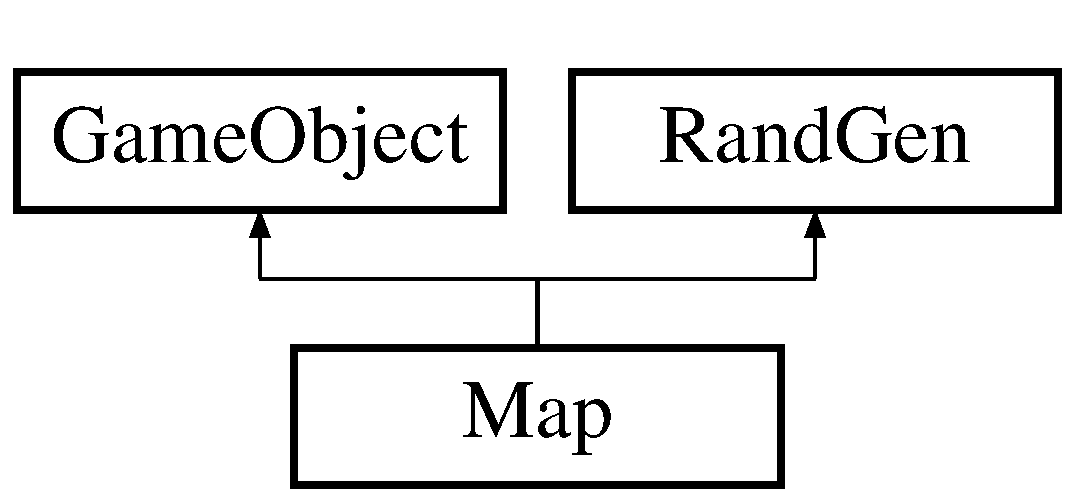
\includegraphics[height=2.000000cm]{class_map}
\end{center}
\end{figure}
\subsection*{Public Member Functions}
\begin{DoxyCompactItemize}
\item 
\mbox{\hyperlink{class_map_a0f5ad0fd4563497b4214038cbca8b582}{Map}} ()
\item 
\mbox{\hyperlink{class_map_aa403fbe09394ccf39747588f5168e3b2}{$\sim$\+Map}} ()
\item 
void \mbox{\hyperlink{class_map_a0f3b846f14a87030cf53d6fd32072cda}{m\+\_\+\+Set\+Up\+Game\+Map}} (sf\+::\+Vector2f dimentions, sf\+::\+Vector2f position)
\item 
void \mbox{\hyperlink{class_map_a2cc424825baa72efdc7ceb1580eabf3a}{m\+\_\+\+Create\+Grid}} ()
\item 
void \mbox{\hyperlink{class_map_a31635a85e9b5d86369ff0765d03dff93}{m\+\_\+\+Assign\+Textures}} (std\+::map$<$ std\+::string, sf\+::\+Texture $>$ \&m\+\_\+\+Texture\+Map)
\item 
void \mbox{\hyperlink{class_map_a50d9a80e029be4f056b8c5d73791b6c4}{m\+\_\+\+Update}} ()
\item 
void \mbox{\hyperlink{class_map_a44b30d85da0d39adb6b144af1ae98616}{m\+\_\+\+Generate\+Map}} ()
\item 
void \mbox{\hyperlink{class_map_a8d88a513b07b30ebd5e0a94ad6537e8b}{m\+\_\+\+Create\+Lake\+For\+Map}} ()
\item 
void \mbox{\hyperlink{class_map_a0fbb42a352131e4815bef949fdcd36d3}{m\+\_\+\+Create\+River\+For\+Map}} ()
\item 
int \mbox{\hyperlink{class_map_a91a657dd319b8fcec0c9ef17702cf2a2}{m\+\_\+\+Get\+Ground\+Level}} ()
\item 
int \mbox{\hyperlink{class_map_a2dd8826757e273671fc952dcd7c9c6b1}{m\+\_\+\+Get\+Current\+Level}} ()
\item 
\mbox{\hyperlink{class_grid}{Grid}} \& \mbox{\hyperlink{class_map_a50cc8967bbc1feed965946bf308e2401}{m\+\_\+\+Get\+Grid}} ()
\item 
sf\+::\+Vector2f \mbox{\hyperlink{class_map_ac8d0317e330bef1da2c965bd24f64412}{m\+\_\+\+Get\+Map\+Upper\+Bounds}} ()
\item 
sf\+::\+Vector2f \mbox{\hyperlink{class_map_adf5933cab79aee80497d72d87a169f62}{m\+\_\+\+Get\+Map\+Lower\+Bounds}} ()
\item 
void \mbox{\hyperlink{class_map_aa65945c61f28808b549a264a3b87219e}{m\+\_\+\+Draw\+Game\+Object}} (sf\+::\+Render\+Window \&window) override
\item 
void \mbox{\hyperlink{class_map_a47f69ae4c316d2efe45bd8a066e982c9}{m\+\_\+\+Draw\+Filter}} (sf\+::\+Vector2f top\+Left, sf\+::\+Vector2f bottom\+Right)
\item 
void \mbox{\hyperlink{class_map_aa44fadcea160127a186720c1ff44e533}{m\+\_\+\+Set\+Object\+Pos}} (float x, float y) override
\item 
void \mbox{\hyperlink{class_map_a024e4daa304e427c35119ae4baa01129}{m\+\_\+\+Check\+For\+Layer\+Change}} (int \&input\+Value)
\item 
void \mbox{\hyperlink{class_map_ae0ac864d328f94d30096184eb71e85cf}{m\+\_\+\+Increase\+Layer}} ()
\item 
void \mbox{\hyperlink{class_map_a59ab8311c6ea6ca42b00ae7e1ec2c10e}{m\+\_\+\+Descrease\+Layer}} ()
\end{DoxyCompactItemize}
\subsection*{Additional Inherited Members}


\subsection{Constructor \& Destructor Documentation}
\mbox{\Hypertarget{class_map_a0f5ad0fd4563497b4214038cbca8b582}\label{class_map_a0f5ad0fd4563497b4214038cbca8b582}} 
\index{Map@{Map}!Map@{Map}}
\index{Map@{Map}!Map@{Map}}
\subsubsection{\texorpdfstring{Map()}{Map()}}
{\footnotesize\ttfamily Map\+::\+Map (\begin{DoxyParamCaption}{ }\end{DoxyParamCaption})}

\mbox{\Hypertarget{class_map_aa403fbe09394ccf39747588f5168e3b2}\label{class_map_aa403fbe09394ccf39747588f5168e3b2}} 
\index{Map@{Map}!````~Map@{$\sim$\+Map}}
\index{````~Map@{$\sim$\+Map}!Map@{Map}}
\subsubsection{\texorpdfstring{$\sim$\+Map()}{~Map()}}
{\footnotesize\ttfamily Map\+::$\sim$\+Map (\begin{DoxyParamCaption}{ }\end{DoxyParamCaption})}



\subsection{Member Function Documentation}
\mbox{\Hypertarget{class_map_a31635a85e9b5d86369ff0765d03dff93}\label{class_map_a31635a85e9b5d86369ff0765d03dff93}} 
\index{Map@{Map}!m\+\_\+\+Assign\+Textures@{m\+\_\+\+Assign\+Textures}}
\index{m\+\_\+\+Assign\+Textures@{m\+\_\+\+Assign\+Textures}!Map@{Map}}
\subsubsection{\texorpdfstring{m\+\_\+\+Assign\+Textures()}{m\_AssignTextures()}}
{\footnotesize\ttfamily void Map\+::m\+\_\+\+Assign\+Textures (\begin{DoxyParamCaption}\item[{std\+::map$<$ std\+::string, sf\+::\+Texture $>$ \&}]{m\+\_\+\+Texture\+Map }\end{DoxyParamCaption})}

\mbox{\Hypertarget{class_map_a024e4daa304e427c35119ae4baa01129}\label{class_map_a024e4daa304e427c35119ae4baa01129}} 
\index{Map@{Map}!m\+\_\+\+Check\+For\+Layer\+Change@{m\+\_\+\+Check\+For\+Layer\+Change}}
\index{m\+\_\+\+Check\+For\+Layer\+Change@{m\+\_\+\+Check\+For\+Layer\+Change}!Map@{Map}}
\subsubsection{\texorpdfstring{m\+\_\+\+Check\+For\+Layer\+Change()}{m\_CheckForLayerChange()}}
{\footnotesize\ttfamily void Map\+::m\+\_\+\+Check\+For\+Layer\+Change (\begin{DoxyParamCaption}\item[{int \&}]{input\+Value }\end{DoxyParamCaption})}

\mbox{\Hypertarget{class_map_a2cc424825baa72efdc7ceb1580eabf3a}\label{class_map_a2cc424825baa72efdc7ceb1580eabf3a}} 
\index{Map@{Map}!m\+\_\+\+Create\+Grid@{m\+\_\+\+Create\+Grid}}
\index{m\+\_\+\+Create\+Grid@{m\+\_\+\+Create\+Grid}!Map@{Map}}
\subsubsection{\texorpdfstring{m\+\_\+\+Create\+Grid()}{m\_CreateGrid()}}
{\footnotesize\ttfamily void Map\+::m\+\_\+\+Create\+Grid (\begin{DoxyParamCaption}{ }\end{DoxyParamCaption})}

\mbox{\Hypertarget{class_map_a8d88a513b07b30ebd5e0a94ad6537e8b}\label{class_map_a8d88a513b07b30ebd5e0a94ad6537e8b}} 
\index{Map@{Map}!m\+\_\+\+Create\+Lake\+For\+Map@{m\+\_\+\+Create\+Lake\+For\+Map}}
\index{m\+\_\+\+Create\+Lake\+For\+Map@{m\+\_\+\+Create\+Lake\+For\+Map}!Map@{Map}}
\subsubsection{\texorpdfstring{m\+\_\+\+Create\+Lake\+For\+Map()}{m\_CreateLakeForMap()}}
{\footnotesize\ttfamily void Map\+::m\+\_\+\+Create\+Lake\+For\+Map (\begin{DoxyParamCaption}{ }\end{DoxyParamCaption})}

\mbox{\Hypertarget{class_map_a0fbb42a352131e4815bef949fdcd36d3}\label{class_map_a0fbb42a352131e4815bef949fdcd36d3}} 
\index{Map@{Map}!m\+\_\+\+Create\+River\+For\+Map@{m\+\_\+\+Create\+River\+For\+Map}}
\index{m\+\_\+\+Create\+River\+For\+Map@{m\+\_\+\+Create\+River\+For\+Map}!Map@{Map}}
\subsubsection{\texorpdfstring{m\+\_\+\+Create\+River\+For\+Map()}{m\_CreateRiverForMap()}}
{\footnotesize\ttfamily void Map\+::m\+\_\+\+Create\+River\+For\+Map (\begin{DoxyParamCaption}{ }\end{DoxyParamCaption})}

\mbox{\Hypertarget{class_map_a59ab8311c6ea6ca42b00ae7e1ec2c10e}\label{class_map_a59ab8311c6ea6ca42b00ae7e1ec2c10e}} 
\index{Map@{Map}!m\+\_\+\+Descrease\+Layer@{m\+\_\+\+Descrease\+Layer}}
\index{m\+\_\+\+Descrease\+Layer@{m\+\_\+\+Descrease\+Layer}!Map@{Map}}
\subsubsection{\texorpdfstring{m\+\_\+\+Descrease\+Layer()}{m\_DescreaseLayer()}}
{\footnotesize\ttfamily void Map\+::m\+\_\+\+Descrease\+Layer (\begin{DoxyParamCaption}{ }\end{DoxyParamCaption})}

\mbox{\Hypertarget{class_map_a47f69ae4c316d2efe45bd8a066e982c9}\label{class_map_a47f69ae4c316d2efe45bd8a066e982c9}} 
\index{Map@{Map}!m\+\_\+\+Draw\+Filter@{m\+\_\+\+Draw\+Filter}}
\index{m\+\_\+\+Draw\+Filter@{m\+\_\+\+Draw\+Filter}!Map@{Map}}
\subsubsection{\texorpdfstring{m\+\_\+\+Draw\+Filter()}{m\_DrawFilter()}}
{\footnotesize\ttfamily void Map\+::m\+\_\+\+Draw\+Filter (\begin{DoxyParamCaption}\item[{sf\+::\+Vector2f}]{top\+Left,  }\item[{sf\+::\+Vector2f}]{bottom\+Right }\end{DoxyParamCaption})\hspace{0.3cm}{\ttfamily [virtual]}}



Implements \mbox{\hyperlink{class_game_object_af1a0662ca445d878b163c4648f90259c}{Game\+Object}}.

\mbox{\Hypertarget{class_map_aa65945c61f28808b549a264a3b87219e}\label{class_map_aa65945c61f28808b549a264a3b87219e}} 
\index{Map@{Map}!m\+\_\+\+Draw\+Game\+Object@{m\+\_\+\+Draw\+Game\+Object}}
\index{m\+\_\+\+Draw\+Game\+Object@{m\+\_\+\+Draw\+Game\+Object}!Map@{Map}}
\subsubsection{\texorpdfstring{m\+\_\+\+Draw\+Game\+Object()}{m\_DrawGameObject()}}
{\footnotesize\ttfamily void Map\+::m\+\_\+\+Draw\+Game\+Object (\begin{DoxyParamCaption}\item[{sf\+::\+Render\+Window \&}]{window }\end{DoxyParamCaption})\hspace{0.3cm}{\ttfamily [override]}, {\ttfamily [virtual]}}



Implements \mbox{\hyperlink{class_game_object_a184ac59fd5167c55a54b50894e5b6721}{Game\+Object}}.

\mbox{\Hypertarget{class_map_a44b30d85da0d39adb6b144af1ae98616}\label{class_map_a44b30d85da0d39adb6b144af1ae98616}} 
\index{Map@{Map}!m\+\_\+\+Generate\+Map@{m\+\_\+\+Generate\+Map}}
\index{m\+\_\+\+Generate\+Map@{m\+\_\+\+Generate\+Map}!Map@{Map}}
\subsubsection{\texorpdfstring{m\+\_\+\+Generate\+Map()}{m\_GenerateMap()}}
{\footnotesize\ttfamily void Map\+::m\+\_\+\+Generate\+Map (\begin{DoxyParamCaption}{ }\end{DoxyParamCaption})}

\mbox{\Hypertarget{class_map_a2dd8826757e273671fc952dcd7c9c6b1}\label{class_map_a2dd8826757e273671fc952dcd7c9c6b1}} 
\index{Map@{Map}!m\+\_\+\+Get\+Current\+Level@{m\+\_\+\+Get\+Current\+Level}}
\index{m\+\_\+\+Get\+Current\+Level@{m\+\_\+\+Get\+Current\+Level}!Map@{Map}}
\subsubsection{\texorpdfstring{m\+\_\+\+Get\+Current\+Level()}{m\_GetCurrentLevel()}}
{\footnotesize\ttfamily int Map\+::m\+\_\+\+Get\+Current\+Level (\begin{DoxyParamCaption}{ }\end{DoxyParamCaption})}

\mbox{\Hypertarget{class_map_a50cc8967bbc1feed965946bf308e2401}\label{class_map_a50cc8967bbc1feed965946bf308e2401}} 
\index{Map@{Map}!m\+\_\+\+Get\+Grid@{m\+\_\+\+Get\+Grid}}
\index{m\+\_\+\+Get\+Grid@{m\+\_\+\+Get\+Grid}!Map@{Map}}
\subsubsection{\texorpdfstring{m\+\_\+\+Get\+Grid()}{m\_GetGrid()}}
{\footnotesize\ttfamily \mbox{\hyperlink{class_grid}{Grid}}\& Map\+::m\+\_\+\+Get\+Grid (\begin{DoxyParamCaption}{ }\end{DoxyParamCaption})}

\mbox{\Hypertarget{class_map_a91a657dd319b8fcec0c9ef17702cf2a2}\label{class_map_a91a657dd319b8fcec0c9ef17702cf2a2}} 
\index{Map@{Map}!m\+\_\+\+Get\+Ground\+Level@{m\+\_\+\+Get\+Ground\+Level}}
\index{m\+\_\+\+Get\+Ground\+Level@{m\+\_\+\+Get\+Ground\+Level}!Map@{Map}}
\subsubsection{\texorpdfstring{m\+\_\+\+Get\+Ground\+Level()}{m\_GetGroundLevel()}}
{\footnotesize\ttfamily int Map\+::m\+\_\+\+Get\+Ground\+Level (\begin{DoxyParamCaption}{ }\end{DoxyParamCaption})}

\mbox{\Hypertarget{class_map_adf5933cab79aee80497d72d87a169f62}\label{class_map_adf5933cab79aee80497d72d87a169f62}} 
\index{Map@{Map}!m\+\_\+\+Get\+Map\+Lower\+Bounds@{m\+\_\+\+Get\+Map\+Lower\+Bounds}}
\index{m\+\_\+\+Get\+Map\+Lower\+Bounds@{m\+\_\+\+Get\+Map\+Lower\+Bounds}!Map@{Map}}
\subsubsection{\texorpdfstring{m\+\_\+\+Get\+Map\+Lower\+Bounds()}{m\_GetMapLowerBounds()}}
{\footnotesize\ttfamily sf\+::\+Vector2f Map\+::m\+\_\+\+Get\+Map\+Lower\+Bounds (\begin{DoxyParamCaption}{ }\end{DoxyParamCaption})}

\mbox{\Hypertarget{class_map_ac8d0317e330bef1da2c965bd24f64412}\label{class_map_ac8d0317e330bef1da2c965bd24f64412}} 
\index{Map@{Map}!m\+\_\+\+Get\+Map\+Upper\+Bounds@{m\+\_\+\+Get\+Map\+Upper\+Bounds}}
\index{m\+\_\+\+Get\+Map\+Upper\+Bounds@{m\+\_\+\+Get\+Map\+Upper\+Bounds}!Map@{Map}}
\subsubsection{\texorpdfstring{m\+\_\+\+Get\+Map\+Upper\+Bounds()}{m\_GetMapUpperBounds()}}
{\footnotesize\ttfamily sf\+::\+Vector2f Map\+::m\+\_\+\+Get\+Map\+Upper\+Bounds (\begin{DoxyParamCaption}{ }\end{DoxyParamCaption})}

\mbox{\Hypertarget{class_map_ae0ac864d328f94d30096184eb71e85cf}\label{class_map_ae0ac864d328f94d30096184eb71e85cf}} 
\index{Map@{Map}!m\+\_\+\+Increase\+Layer@{m\+\_\+\+Increase\+Layer}}
\index{m\+\_\+\+Increase\+Layer@{m\+\_\+\+Increase\+Layer}!Map@{Map}}
\subsubsection{\texorpdfstring{m\+\_\+\+Increase\+Layer()}{m\_IncreaseLayer()}}
{\footnotesize\ttfamily void Map\+::m\+\_\+\+Increase\+Layer (\begin{DoxyParamCaption}{ }\end{DoxyParamCaption})}

\mbox{\Hypertarget{class_map_aa44fadcea160127a186720c1ff44e533}\label{class_map_aa44fadcea160127a186720c1ff44e533}} 
\index{Map@{Map}!m\+\_\+\+Set\+Object\+Pos@{m\+\_\+\+Set\+Object\+Pos}}
\index{m\+\_\+\+Set\+Object\+Pos@{m\+\_\+\+Set\+Object\+Pos}!Map@{Map}}
\subsubsection{\texorpdfstring{m\+\_\+\+Set\+Object\+Pos()}{m\_SetObjectPos()}}
{\footnotesize\ttfamily void Map\+::m\+\_\+\+Set\+Object\+Pos (\begin{DoxyParamCaption}\item[{float}]{x,  }\item[{float}]{y }\end{DoxyParamCaption})\hspace{0.3cm}{\ttfamily [override]}, {\ttfamily [virtual]}}



Implements \mbox{\hyperlink{class_game_object_ad1f8ea8eb3673b1af8215bf92cdc0df8}{Game\+Object}}.

\mbox{\Hypertarget{class_map_a0f3b846f14a87030cf53d6fd32072cda}\label{class_map_a0f3b846f14a87030cf53d6fd32072cda}} 
\index{Map@{Map}!m\+\_\+\+Set\+Up\+Game\+Map@{m\+\_\+\+Set\+Up\+Game\+Map}}
\index{m\+\_\+\+Set\+Up\+Game\+Map@{m\+\_\+\+Set\+Up\+Game\+Map}!Map@{Map}}
\subsubsection{\texorpdfstring{m\+\_\+\+Set\+Up\+Game\+Map()}{m\_SetUpGameMap()}}
{\footnotesize\ttfamily void Map\+::m\+\_\+\+Set\+Up\+Game\+Map (\begin{DoxyParamCaption}\item[{sf\+::\+Vector2f}]{dimentions,  }\item[{sf\+::\+Vector2f}]{position }\end{DoxyParamCaption})}

\mbox{\Hypertarget{class_map_a50d9a80e029be4f056b8c5d73791b6c4}\label{class_map_a50d9a80e029be4f056b8c5d73791b6c4}} 
\index{Map@{Map}!m\+\_\+\+Update@{m\+\_\+\+Update}}
\index{m\+\_\+\+Update@{m\+\_\+\+Update}!Map@{Map}}
\subsubsection{\texorpdfstring{m\+\_\+\+Update()}{m\_Update()}}
{\footnotesize\ttfamily void Map\+::m\+\_\+\+Update (\begin{DoxyParamCaption}{ }\end{DoxyParamCaption})\hspace{0.3cm}{\ttfamily [virtual]}}



Implements \mbox{\hyperlink{class_game_object_a3af5a7b470e09f13a1422439fc6a9ba8}{Game\+Object}}.



The documentation for this class was generated from the following file\+:\begin{DoxyCompactItemize}
\item 
inc/\mbox{\hyperlink{_game_map_8h}{Game\+Map.\+h}}\end{DoxyCompactItemize}

\hypertarget{class_mouse}{}\section{Mouse Class Reference}
\label{class_mouse}\index{Mouse@{Mouse}}


{\ttfamily \#include $<$Mouse.\+h$>$}

\subsection*{Public Member Functions}
\begin{DoxyCompactItemize}
\item 
\mbox{\hyperlink{class_mouse_a99024d3700d649ae19c1537b42a3e86d}{Mouse}} ()
\item 
\mbox{\hyperlink{class_mouse_afdf7d8abef29c10be77ead773f964f4f}{$\sim$\+Mouse}} ()
\item 
void \mbox{\hyperlink{class_mouse_a3bd0290c0d6d6d4c5024ad50aac97384}{m\+\_\+\+Set\+Mouse\+Pos}} (sf\+::\+Render\+Window \&window)
\item 
sf\+::\+Vector2f \mbox{\hyperlink{class_mouse_a3cecb21e004a7543f862adeb1f99668f}{m\+\_\+\+Get\+Mouse\+Pos}} ()
\item 
bool \mbox{\hyperlink{class_mouse_aa80965ead15bff808a7ac925808fe2ef}{m\+\_\+\+Get\+L\+M\+B\+Down}} (sf\+::\+Vector2f map\+Upper\+Bounds, sf\+::\+Vector2f map\+Lower\+Bounds)
\item 
void \mbox{\hyperlink{class_mouse_a04d21fe5944d4ba7460c74d0f6e56bb2}{m\+\_\+\+Create\+Selection\+Box}} ()
\item 
sf\+::\+Vector2f \mbox{\hyperlink{class_mouse_a11ee7162a00ebdde0fd089189507a0a1}{m\+\_\+\+Get\+Top\+Left\+Selection\+Box}} ()
\item 
sf\+::\+Vector2f \mbox{\hyperlink{class_mouse_a355172dc80aba80651fa57dd53efd68c}{m\+\_\+\+Get\+Bottom\+Right\+Selection\+Box}} ()
\item 
void \mbox{\hyperlink{class_mouse_a4562b08f5f21a00fead0196d5a4c34ea}{m\+\_\+\+Draw\+Selection\+Box}} (sf\+::\+Render\+Window \&window)
\item 
void \mbox{\hyperlink{class_mouse_ac668f6d214750b0c426486dd56de5bb0}{m\+\_\+\+Assign\+Tool\+Tip\+Font}} (sf\+::\+Font new\+Font)
\item 
void \mbox{\hyperlink{class_mouse_ab3b5422cbcf9eae16684998912f20b52}{m\+\_\+\+Update\+Tooltip}} (std\+::string data\+To\+Display, sf\+::\+Vector2f view\+Pos, sf\+::\+Vector2f view\+Size)
\item 
void \mbox{\hyperlink{class_mouse_ad1b3f025265e9f4823f19a7f4adc9add}{m\+\_\+\+Draw\+Tool\+Tip}} (sf\+::\+Render\+Window \&window)
\end{DoxyCompactItemize}


\subsection{Constructor \& Destructor Documentation}
\mbox{\Hypertarget{class_mouse_a99024d3700d649ae19c1537b42a3e86d}\label{class_mouse_a99024d3700d649ae19c1537b42a3e86d}} 
\index{Mouse@{Mouse}!Mouse@{Mouse}}
\index{Mouse@{Mouse}!Mouse@{Mouse}}
\subsubsection{\texorpdfstring{Mouse()}{Mouse()}}
{\footnotesize\ttfamily Mouse\+::\+Mouse (\begin{DoxyParamCaption}{ }\end{DoxyParamCaption})}

\mbox{\Hypertarget{class_mouse_afdf7d8abef29c10be77ead773f964f4f}\label{class_mouse_afdf7d8abef29c10be77ead773f964f4f}} 
\index{Mouse@{Mouse}!````~Mouse@{$\sim$\+Mouse}}
\index{````~Mouse@{$\sim$\+Mouse}!Mouse@{Mouse}}
\subsubsection{\texorpdfstring{$\sim$\+Mouse()}{~Mouse()}}
{\footnotesize\ttfamily Mouse\+::$\sim$\+Mouse (\begin{DoxyParamCaption}{ }\end{DoxyParamCaption})}



\subsection{Member Function Documentation}
\mbox{\Hypertarget{class_mouse_ac668f6d214750b0c426486dd56de5bb0}\label{class_mouse_ac668f6d214750b0c426486dd56de5bb0}} 
\index{Mouse@{Mouse}!m\+\_\+\+Assign\+Tool\+Tip\+Font@{m\+\_\+\+Assign\+Tool\+Tip\+Font}}
\index{m\+\_\+\+Assign\+Tool\+Tip\+Font@{m\+\_\+\+Assign\+Tool\+Tip\+Font}!Mouse@{Mouse}}
\subsubsection{\texorpdfstring{m\+\_\+\+Assign\+Tool\+Tip\+Font()}{m\_AssignToolTipFont()}}
{\footnotesize\ttfamily void Mouse\+::m\+\_\+\+Assign\+Tool\+Tip\+Font (\begin{DoxyParamCaption}\item[{sf\+::\+Font}]{new\+Font }\end{DoxyParamCaption})}

\mbox{\Hypertarget{class_mouse_a04d21fe5944d4ba7460c74d0f6e56bb2}\label{class_mouse_a04d21fe5944d4ba7460c74d0f6e56bb2}} 
\index{Mouse@{Mouse}!m\+\_\+\+Create\+Selection\+Box@{m\+\_\+\+Create\+Selection\+Box}}
\index{m\+\_\+\+Create\+Selection\+Box@{m\+\_\+\+Create\+Selection\+Box}!Mouse@{Mouse}}
\subsubsection{\texorpdfstring{m\+\_\+\+Create\+Selection\+Box()}{m\_CreateSelectionBox()}}
{\footnotesize\ttfamily void Mouse\+::m\+\_\+\+Create\+Selection\+Box (\begin{DoxyParamCaption}{ }\end{DoxyParamCaption})}

\mbox{\Hypertarget{class_mouse_a4562b08f5f21a00fead0196d5a4c34ea}\label{class_mouse_a4562b08f5f21a00fead0196d5a4c34ea}} 
\index{Mouse@{Mouse}!m\+\_\+\+Draw\+Selection\+Box@{m\+\_\+\+Draw\+Selection\+Box}}
\index{m\+\_\+\+Draw\+Selection\+Box@{m\+\_\+\+Draw\+Selection\+Box}!Mouse@{Mouse}}
\subsubsection{\texorpdfstring{m\+\_\+\+Draw\+Selection\+Box()}{m\_DrawSelectionBox()}}
{\footnotesize\ttfamily void Mouse\+::m\+\_\+\+Draw\+Selection\+Box (\begin{DoxyParamCaption}\item[{sf\+::\+Render\+Window \&}]{window }\end{DoxyParamCaption})}

\mbox{\Hypertarget{class_mouse_ad1b3f025265e9f4823f19a7f4adc9add}\label{class_mouse_ad1b3f025265e9f4823f19a7f4adc9add}} 
\index{Mouse@{Mouse}!m\+\_\+\+Draw\+Tool\+Tip@{m\+\_\+\+Draw\+Tool\+Tip}}
\index{m\+\_\+\+Draw\+Tool\+Tip@{m\+\_\+\+Draw\+Tool\+Tip}!Mouse@{Mouse}}
\subsubsection{\texorpdfstring{m\+\_\+\+Draw\+Tool\+Tip()}{m\_DrawToolTip()}}
{\footnotesize\ttfamily void Mouse\+::m\+\_\+\+Draw\+Tool\+Tip (\begin{DoxyParamCaption}\item[{sf\+::\+Render\+Window \&}]{window }\end{DoxyParamCaption})}

\mbox{\Hypertarget{class_mouse_a355172dc80aba80651fa57dd53efd68c}\label{class_mouse_a355172dc80aba80651fa57dd53efd68c}} 
\index{Mouse@{Mouse}!m\+\_\+\+Get\+Bottom\+Right\+Selection\+Box@{m\+\_\+\+Get\+Bottom\+Right\+Selection\+Box}}
\index{m\+\_\+\+Get\+Bottom\+Right\+Selection\+Box@{m\+\_\+\+Get\+Bottom\+Right\+Selection\+Box}!Mouse@{Mouse}}
\subsubsection{\texorpdfstring{m\+\_\+\+Get\+Bottom\+Right\+Selection\+Box()}{m\_GetBottomRightSelectionBox()}}
{\footnotesize\ttfamily sf\+::\+Vector2f Mouse\+::m\+\_\+\+Get\+Bottom\+Right\+Selection\+Box (\begin{DoxyParamCaption}{ }\end{DoxyParamCaption})}

\mbox{\Hypertarget{class_mouse_aa80965ead15bff808a7ac925808fe2ef}\label{class_mouse_aa80965ead15bff808a7ac925808fe2ef}} 
\index{Mouse@{Mouse}!m\+\_\+\+Get\+L\+M\+B\+Down@{m\+\_\+\+Get\+L\+M\+B\+Down}}
\index{m\+\_\+\+Get\+L\+M\+B\+Down@{m\+\_\+\+Get\+L\+M\+B\+Down}!Mouse@{Mouse}}
\subsubsection{\texorpdfstring{m\+\_\+\+Get\+L\+M\+B\+Down()}{m\_GetLMBDown()}}
{\footnotesize\ttfamily bool Mouse\+::m\+\_\+\+Get\+L\+M\+B\+Down (\begin{DoxyParamCaption}\item[{sf\+::\+Vector2f}]{map\+Upper\+Bounds,  }\item[{sf\+::\+Vector2f}]{map\+Lower\+Bounds }\end{DoxyParamCaption})}

\mbox{\Hypertarget{class_mouse_a3cecb21e004a7543f862adeb1f99668f}\label{class_mouse_a3cecb21e004a7543f862adeb1f99668f}} 
\index{Mouse@{Mouse}!m\+\_\+\+Get\+Mouse\+Pos@{m\+\_\+\+Get\+Mouse\+Pos}}
\index{m\+\_\+\+Get\+Mouse\+Pos@{m\+\_\+\+Get\+Mouse\+Pos}!Mouse@{Mouse}}
\subsubsection{\texorpdfstring{m\+\_\+\+Get\+Mouse\+Pos()}{m\_GetMousePos()}}
{\footnotesize\ttfamily sf\+::\+Vector2f Mouse\+::m\+\_\+\+Get\+Mouse\+Pos (\begin{DoxyParamCaption}{ }\end{DoxyParamCaption})}

\mbox{\Hypertarget{class_mouse_a11ee7162a00ebdde0fd089189507a0a1}\label{class_mouse_a11ee7162a00ebdde0fd089189507a0a1}} 
\index{Mouse@{Mouse}!m\+\_\+\+Get\+Top\+Left\+Selection\+Box@{m\+\_\+\+Get\+Top\+Left\+Selection\+Box}}
\index{m\+\_\+\+Get\+Top\+Left\+Selection\+Box@{m\+\_\+\+Get\+Top\+Left\+Selection\+Box}!Mouse@{Mouse}}
\subsubsection{\texorpdfstring{m\+\_\+\+Get\+Top\+Left\+Selection\+Box()}{m\_GetTopLeftSelectionBox()}}
{\footnotesize\ttfamily sf\+::\+Vector2f Mouse\+::m\+\_\+\+Get\+Top\+Left\+Selection\+Box (\begin{DoxyParamCaption}{ }\end{DoxyParamCaption})}

\mbox{\Hypertarget{class_mouse_a3bd0290c0d6d6d4c5024ad50aac97384}\label{class_mouse_a3bd0290c0d6d6d4c5024ad50aac97384}} 
\index{Mouse@{Mouse}!m\+\_\+\+Set\+Mouse\+Pos@{m\+\_\+\+Set\+Mouse\+Pos}}
\index{m\+\_\+\+Set\+Mouse\+Pos@{m\+\_\+\+Set\+Mouse\+Pos}!Mouse@{Mouse}}
\subsubsection{\texorpdfstring{m\+\_\+\+Set\+Mouse\+Pos()}{m\_SetMousePos()}}
{\footnotesize\ttfamily void Mouse\+::m\+\_\+\+Set\+Mouse\+Pos (\begin{DoxyParamCaption}\item[{sf\+::\+Render\+Window \&}]{window }\end{DoxyParamCaption})}

\mbox{\Hypertarget{class_mouse_ab3b5422cbcf9eae16684998912f20b52}\label{class_mouse_ab3b5422cbcf9eae16684998912f20b52}} 
\index{Mouse@{Mouse}!m\+\_\+\+Update\+Tooltip@{m\+\_\+\+Update\+Tooltip}}
\index{m\+\_\+\+Update\+Tooltip@{m\+\_\+\+Update\+Tooltip}!Mouse@{Mouse}}
\subsubsection{\texorpdfstring{m\+\_\+\+Update\+Tooltip()}{m\_UpdateTooltip()}}
{\footnotesize\ttfamily void Mouse\+::m\+\_\+\+Update\+Tooltip (\begin{DoxyParamCaption}\item[{std\+::string}]{data\+To\+Display,  }\item[{sf\+::\+Vector2f}]{view\+Pos,  }\item[{sf\+::\+Vector2f}]{view\+Size }\end{DoxyParamCaption})}



The documentation for this class was generated from the following file\+:\begin{DoxyCompactItemize}
\item 
inc/\mbox{\hyperlink{_mouse_8h}{Mouse.\+h}}\end{DoxyCompactItemize}

\hypertarget{class_pathfinding}{}\section{Pathfinding Class Reference}
\label{class_pathfinding}\index{Pathfinding@{Pathfinding}}


{\ttfamily \#include $<$Pathfinding.\+h$>$}

\subsection*{Public Member Functions}
\begin{DoxyCompactItemize}
\item 
\mbox{\hyperlink{class_pathfinding_aae14d204c5f9ee6b184764f874711341}{Pathfinding}} ()
\item 
\mbox{\hyperlink{class_pathfinding_a1869823af12d301105cf1cedbe9a8dc5}{$\sim$\+Pathfinding}} ()
\item 
void \mbox{\hyperlink{class_pathfinding_a4c5a8788f066f2b91ab52958b211f28d}{m\+\_\+\+Init\+Algorithm}} (\mbox{\hyperlink{class_cells}{Cells}} $\ast$start\+Cell, \mbox{\hyperlink{class_cells}{Cells}} $\ast$end\+Cell)
\item 
void \mbox{\hyperlink{class_pathfinding_a423a7763b0990f4143ffcc517ddf2c29}{m\+\_\+\+Run\+A\+Star\+Algorithm}} ()
\item 
void \mbox{\hyperlink{class_pathfinding_a15896b383f998b1fd8e996b11abfa17a}{m\+\_\+\+Run\+A\+Star\+Algorithm}} (std\+::vector$<$ \mbox{\hyperlink{_cells_8h_adc5e4636eae42cdad2a070c6adbd9daf}{tile\+Set}} $>$ obstructions)
\item 
void \mbox{\hyperlink{class_pathfinding_a0dcc4744c8892ca16c6f685f8c534645}{m\+\_\+\+Run\+A\+Star\+Algorithm}} (std\+::vector$<$ \mbox{\hyperlink{_cells_8h_adc5e4636eae42cdad2a070c6adbd9daf}{tile\+Set}} $>$ obstructions, bool add\+Colour)
\item 
sf\+::\+Vector2f \mbox{\hyperlink{class_pathfinding_a17051c2f3466edb6299444e87d6033fc}{m\+\_\+\+Calc\+Dist}} (\mbox{\hyperlink{class_cells}{Cells}} $\ast$point\+One, \mbox{\hyperlink{class_cells}{Cells}} $\ast$point\+Two)
\item 
int \mbox{\hyperlink{class_pathfinding_a717eed7fdd1fe504da934e575dfa1443}{m\+\_\+\+Calculate\+G\+Score}} (\mbox{\hyperlink{class_cells}{Cells}} $\ast$start\+Cell, \mbox{\hyperlink{class_cells}{Cells}} $\ast$current\+Cell)
\item 
int \mbox{\hyperlink{class_pathfinding_ad89518accab0433588c8e8ffa63b0d16}{m\+\_\+\+Calculate\+H\+Score}} (\mbox{\hyperlink{class_cells}{Cells}} $\ast$current\+Cell, \mbox{\hyperlink{class_cells}{Cells}} $\ast$end\+Cell)
\item 
int \mbox{\hyperlink{class_pathfinding_a5df6c9a7c337bf4b416ff61dcf57dd98}{m\+\_\+\+Calculate\+F\+Score}} (\mbox{\hyperlink{class_cells}{Cells}} $\ast$current\+Cell)
\item 
void \mbox{\hyperlink{class_pathfinding_abca4c4bbc051a99323d29106127fb389}{m\+\_\+\+Trace\+Path}} ()
\item 
std\+::deque$<$ \mbox{\hyperlink{class_cells}{Cells}} $\ast$ $>$ \mbox{\hyperlink{class_pathfinding_a287047690fb8d2f4d72dbda8365b1f84}{m\+\_\+\+Get\+Current\+Path}} ()
\item 
bool \mbox{\hyperlink{class_pathfinding_a6d557c82148fd127b2c53add89158c5e}{m\+\_\+\+Check\+For\+Completion}} ()
\end{DoxyCompactItemize}


\subsection{Constructor \& Destructor Documentation}
\mbox{\Hypertarget{class_pathfinding_aae14d204c5f9ee6b184764f874711341}\label{class_pathfinding_aae14d204c5f9ee6b184764f874711341}} 
\index{Pathfinding@{Pathfinding}!Pathfinding@{Pathfinding}}
\index{Pathfinding@{Pathfinding}!Pathfinding@{Pathfinding}}
\subsubsection{\texorpdfstring{Pathfinding()}{Pathfinding()}}
{\footnotesize\ttfamily Pathfinding\+::\+Pathfinding (\begin{DoxyParamCaption}{ }\end{DoxyParamCaption})}

\mbox{\Hypertarget{class_pathfinding_a1869823af12d301105cf1cedbe9a8dc5}\label{class_pathfinding_a1869823af12d301105cf1cedbe9a8dc5}} 
\index{Pathfinding@{Pathfinding}!````~Pathfinding@{$\sim$\+Pathfinding}}
\index{````~Pathfinding@{$\sim$\+Pathfinding}!Pathfinding@{Pathfinding}}
\subsubsection{\texorpdfstring{$\sim$\+Pathfinding()}{~Pathfinding()}}
{\footnotesize\ttfamily Pathfinding\+::$\sim$\+Pathfinding (\begin{DoxyParamCaption}{ }\end{DoxyParamCaption})}



\subsection{Member Function Documentation}
\mbox{\Hypertarget{class_pathfinding_a17051c2f3466edb6299444e87d6033fc}\label{class_pathfinding_a17051c2f3466edb6299444e87d6033fc}} 
\index{Pathfinding@{Pathfinding}!m\+\_\+\+Calc\+Dist@{m\+\_\+\+Calc\+Dist}}
\index{m\+\_\+\+Calc\+Dist@{m\+\_\+\+Calc\+Dist}!Pathfinding@{Pathfinding}}
\subsubsection{\texorpdfstring{m\+\_\+\+Calc\+Dist()}{m\_CalcDist()}}
{\footnotesize\ttfamily sf\+::\+Vector2f Pathfinding\+::m\+\_\+\+Calc\+Dist (\begin{DoxyParamCaption}\item[{\mbox{\hyperlink{class_cells}{Cells}} $\ast$}]{point\+One,  }\item[{\mbox{\hyperlink{class_cells}{Cells}} $\ast$}]{point\+Two }\end{DoxyParamCaption})}

\mbox{\Hypertarget{class_pathfinding_a5df6c9a7c337bf4b416ff61dcf57dd98}\label{class_pathfinding_a5df6c9a7c337bf4b416ff61dcf57dd98}} 
\index{Pathfinding@{Pathfinding}!m\+\_\+\+Calculate\+F\+Score@{m\+\_\+\+Calculate\+F\+Score}}
\index{m\+\_\+\+Calculate\+F\+Score@{m\+\_\+\+Calculate\+F\+Score}!Pathfinding@{Pathfinding}}
\subsubsection{\texorpdfstring{m\+\_\+\+Calculate\+F\+Score()}{m\_CalculateFScore()}}
{\footnotesize\ttfamily int Pathfinding\+::m\+\_\+\+Calculate\+F\+Score (\begin{DoxyParamCaption}\item[{\mbox{\hyperlink{class_cells}{Cells}} $\ast$}]{current\+Cell }\end{DoxyParamCaption})}

\mbox{\Hypertarget{class_pathfinding_a717eed7fdd1fe504da934e575dfa1443}\label{class_pathfinding_a717eed7fdd1fe504da934e575dfa1443}} 
\index{Pathfinding@{Pathfinding}!m\+\_\+\+Calculate\+G\+Score@{m\+\_\+\+Calculate\+G\+Score}}
\index{m\+\_\+\+Calculate\+G\+Score@{m\+\_\+\+Calculate\+G\+Score}!Pathfinding@{Pathfinding}}
\subsubsection{\texorpdfstring{m\+\_\+\+Calculate\+G\+Score()}{m\_CalculateGScore()}}
{\footnotesize\ttfamily int Pathfinding\+::m\+\_\+\+Calculate\+G\+Score (\begin{DoxyParamCaption}\item[{\mbox{\hyperlink{class_cells}{Cells}} $\ast$}]{start\+Cell,  }\item[{\mbox{\hyperlink{class_cells}{Cells}} $\ast$}]{current\+Cell }\end{DoxyParamCaption})}

\mbox{\Hypertarget{class_pathfinding_ad89518accab0433588c8e8ffa63b0d16}\label{class_pathfinding_ad89518accab0433588c8e8ffa63b0d16}} 
\index{Pathfinding@{Pathfinding}!m\+\_\+\+Calculate\+H\+Score@{m\+\_\+\+Calculate\+H\+Score}}
\index{m\+\_\+\+Calculate\+H\+Score@{m\+\_\+\+Calculate\+H\+Score}!Pathfinding@{Pathfinding}}
\subsubsection{\texorpdfstring{m\+\_\+\+Calculate\+H\+Score()}{m\_CalculateHScore()}}
{\footnotesize\ttfamily int Pathfinding\+::m\+\_\+\+Calculate\+H\+Score (\begin{DoxyParamCaption}\item[{\mbox{\hyperlink{class_cells}{Cells}} $\ast$}]{current\+Cell,  }\item[{\mbox{\hyperlink{class_cells}{Cells}} $\ast$}]{end\+Cell }\end{DoxyParamCaption})}

\mbox{\Hypertarget{class_pathfinding_a6d557c82148fd127b2c53add89158c5e}\label{class_pathfinding_a6d557c82148fd127b2c53add89158c5e}} 
\index{Pathfinding@{Pathfinding}!m\+\_\+\+Check\+For\+Completion@{m\+\_\+\+Check\+For\+Completion}}
\index{m\+\_\+\+Check\+For\+Completion@{m\+\_\+\+Check\+For\+Completion}!Pathfinding@{Pathfinding}}
\subsubsection{\texorpdfstring{m\+\_\+\+Check\+For\+Completion()}{m\_CheckForCompletion()}}
{\footnotesize\ttfamily bool Pathfinding\+::m\+\_\+\+Check\+For\+Completion (\begin{DoxyParamCaption}{ }\end{DoxyParamCaption})}

\mbox{\Hypertarget{class_pathfinding_a287047690fb8d2f4d72dbda8365b1f84}\label{class_pathfinding_a287047690fb8d2f4d72dbda8365b1f84}} 
\index{Pathfinding@{Pathfinding}!m\+\_\+\+Get\+Current\+Path@{m\+\_\+\+Get\+Current\+Path}}
\index{m\+\_\+\+Get\+Current\+Path@{m\+\_\+\+Get\+Current\+Path}!Pathfinding@{Pathfinding}}
\subsubsection{\texorpdfstring{m\+\_\+\+Get\+Current\+Path()}{m\_GetCurrentPath()}}
{\footnotesize\ttfamily std\+::deque$<$\mbox{\hyperlink{class_cells}{Cells}}$\ast$$>$ Pathfinding\+::m\+\_\+\+Get\+Current\+Path (\begin{DoxyParamCaption}{ }\end{DoxyParamCaption})}

\mbox{\Hypertarget{class_pathfinding_a4c5a8788f066f2b91ab52958b211f28d}\label{class_pathfinding_a4c5a8788f066f2b91ab52958b211f28d}} 
\index{Pathfinding@{Pathfinding}!m\+\_\+\+Init\+Algorithm@{m\+\_\+\+Init\+Algorithm}}
\index{m\+\_\+\+Init\+Algorithm@{m\+\_\+\+Init\+Algorithm}!Pathfinding@{Pathfinding}}
\subsubsection{\texorpdfstring{m\+\_\+\+Init\+Algorithm()}{m\_InitAlgorithm()}}
{\footnotesize\ttfamily void Pathfinding\+::m\+\_\+\+Init\+Algorithm (\begin{DoxyParamCaption}\item[{\mbox{\hyperlink{class_cells}{Cells}} $\ast$}]{start\+Cell,  }\item[{\mbox{\hyperlink{class_cells}{Cells}} $\ast$}]{end\+Cell }\end{DoxyParamCaption})}

\mbox{\Hypertarget{class_pathfinding_a423a7763b0990f4143ffcc517ddf2c29}\label{class_pathfinding_a423a7763b0990f4143ffcc517ddf2c29}} 
\index{Pathfinding@{Pathfinding}!m\+\_\+\+Run\+A\+Star\+Algorithm@{m\+\_\+\+Run\+A\+Star\+Algorithm}}
\index{m\+\_\+\+Run\+A\+Star\+Algorithm@{m\+\_\+\+Run\+A\+Star\+Algorithm}!Pathfinding@{Pathfinding}}
\subsubsection{\texorpdfstring{m\+\_\+\+Run\+A\+Star\+Algorithm()}{m\_RunAStarAlgorithm()}\hspace{0.1cm}{\footnotesize\ttfamily [1/3]}}
{\footnotesize\ttfamily void Pathfinding\+::m\+\_\+\+Run\+A\+Star\+Algorithm (\begin{DoxyParamCaption}{ }\end{DoxyParamCaption})}

\mbox{\Hypertarget{class_pathfinding_a15896b383f998b1fd8e996b11abfa17a}\label{class_pathfinding_a15896b383f998b1fd8e996b11abfa17a}} 
\index{Pathfinding@{Pathfinding}!m\+\_\+\+Run\+A\+Star\+Algorithm@{m\+\_\+\+Run\+A\+Star\+Algorithm}}
\index{m\+\_\+\+Run\+A\+Star\+Algorithm@{m\+\_\+\+Run\+A\+Star\+Algorithm}!Pathfinding@{Pathfinding}}
\subsubsection{\texorpdfstring{m\+\_\+\+Run\+A\+Star\+Algorithm()}{m\_RunAStarAlgorithm()}\hspace{0.1cm}{\footnotesize\ttfamily [2/3]}}
{\footnotesize\ttfamily void Pathfinding\+::m\+\_\+\+Run\+A\+Star\+Algorithm (\begin{DoxyParamCaption}\item[{std\+::vector$<$ \mbox{\hyperlink{_cells_8h_adc5e4636eae42cdad2a070c6adbd9daf}{tile\+Set}} $>$}]{obstructions }\end{DoxyParamCaption})}

\mbox{\Hypertarget{class_pathfinding_a0dcc4744c8892ca16c6f685f8c534645}\label{class_pathfinding_a0dcc4744c8892ca16c6f685f8c534645}} 
\index{Pathfinding@{Pathfinding}!m\+\_\+\+Run\+A\+Star\+Algorithm@{m\+\_\+\+Run\+A\+Star\+Algorithm}}
\index{m\+\_\+\+Run\+A\+Star\+Algorithm@{m\+\_\+\+Run\+A\+Star\+Algorithm}!Pathfinding@{Pathfinding}}
\subsubsection{\texorpdfstring{m\+\_\+\+Run\+A\+Star\+Algorithm()}{m\_RunAStarAlgorithm()}\hspace{0.1cm}{\footnotesize\ttfamily [3/3]}}
{\footnotesize\ttfamily void Pathfinding\+::m\+\_\+\+Run\+A\+Star\+Algorithm (\begin{DoxyParamCaption}\item[{std\+::vector$<$ \mbox{\hyperlink{_cells_8h_adc5e4636eae42cdad2a070c6adbd9daf}{tile\+Set}} $>$}]{obstructions,  }\item[{bool}]{add\+Colour }\end{DoxyParamCaption})}

\mbox{\Hypertarget{class_pathfinding_abca4c4bbc051a99323d29106127fb389}\label{class_pathfinding_abca4c4bbc051a99323d29106127fb389}} 
\index{Pathfinding@{Pathfinding}!m\+\_\+\+Trace\+Path@{m\+\_\+\+Trace\+Path}}
\index{m\+\_\+\+Trace\+Path@{m\+\_\+\+Trace\+Path}!Pathfinding@{Pathfinding}}
\subsubsection{\texorpdfstring{m\+\_\+\+Trace\+Path()}{m\_TracePath()}}
{\footnotesize\ttfamily void Pathfinding\+::m\+\_\+\+Trace\+Path (\begin{DoxyParamCaption}{ }\end{DoxyParamCaption})}



The documentation for this class was generated from the following file\+:\begin{DoxyCompactItemize}
\item 
inc/\mbox{\hyperlink{_pathfinding_8h}{Pathfinding.\+h}}\end{DoxyCompactItemize}

\hypertarget{class_rand_gen}{}\section{Rand\+Gen Class Reference}
\label{class_rand_gen}\index{Rand\+Gen@{Rand\+Gen}}


{\ttfamily \#include $<$Rand\+Gen.\+h$>$}

Inheritance diagram for Rand\+Gen\+:\begin{figure}[H]
\begin{center}
\leavevmode
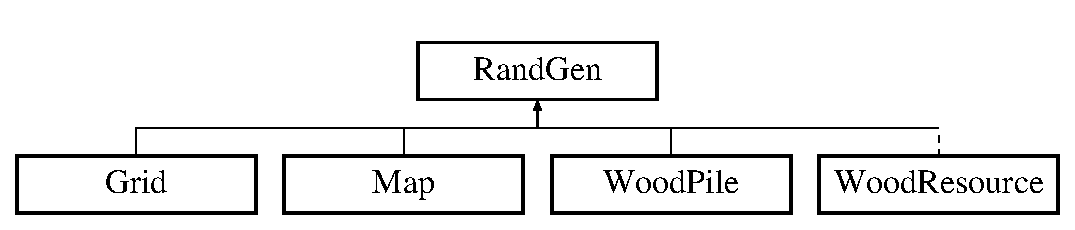
\includegraphics[height=2.000000cm]{class_rand_gen}
\end{center}
\end{figure}
\subsection*{Public Member Functions}
\begin{DoxyCompactItemize}
\item 
int \mbox{\hyperlink{class_rand_gen_aa82bd09942b993c8900e581feca86358}{m\+\_\+\+Generate\+Int}} (int min, int max)
\item 
int \mbox{\hyperlink{class_rand_gen_a5d786a628d29d51aae40a9df78c1f928}{m\+\_\+\+Generate\+Int}} (int min, int max, bool print)
\end{DoxyCompactItemize}


\subsection{Member Function Documentation}
\mbox{\Hypertarget{class_rand_gen_aa82bd09942b993c8900e581feca86358}\label{class_rand_gen_aa82bd09942b993c8900e581feca86358}} 
\index{Rand\+Gen@{Rand\+Gen}!m\+\_\+\+Generate\+Int@{m\+\_\+\+Generate\+Int}}
\index{m\+\_\+\+Generate\+Int@{m\+\_\+\+Generate\+Int}!Rand\+Gen@{Rand\+Gen}}
\subsubsection{\texorpdfstring{m\+\_\+\+Generate\+Int()}{m\_GenerateInt()}\hspace{0.1cm}{\footnotesize\ttfamily [1/2]}}
{\footnotesize\ttfamily int Rand\+Gen\+::m\+\_\+\+Generate\+Int (\begin{DoxyParamCaption}\item[{int}]{min,  }\item[{int}]{max }\end{DoxyParamCaption})}

\mbox{\Hypertarget{class_rand_gen_a5d786a628d29d51aae40a9df78c1f928}\label{class_rand_gen_a5d786a628d29d51aae40a9df78c1f928}} 
\index{Rand\+Gen@{Rand\+Gen}!m\+\_\+\+Generate\+Int@{m\+\_\+\+Generate\+Int}}
\index{m\+\_\+\+Generate\+Int@{m\+\_\+\+Generate\+Int}!Rand\+Gen@{Rand\+Gen}}
\subsubsection{\texorpdfstring{m\+\_\+\+Generate\+Int()}{m\_GenerateInt()}\hspace{0.1cm}{\footnotesize\ttfamily [2/2]}}
{\footnotesize\ttfamily int Rand\+Gen\+::m\+\_\+\+Generate\+Int (\begin{DoxyParamCaption}\item[{int}]{min,  }\item[{int}]{max,  }\item[{bool}]{print }\end{DoxyParamCaption})}



The documentation for this class was generated from the following file\+:\begin{DoxyCompactItemize}
\item 
inc/\mbox{\hyperlink{_rand_gen_8h}{Rand\+Gen.\+h}}\end{DoxyCompactItemize}

\hypertarget{class_resource_management}{}\section{Resource\+Management Class Reference}
\label{class_resource_management}\index{Resource\+Management@{Resource\+Management}}


{\ttfamily \#include $<$Resource\+Management.\+h$>$}

\subsection*{Public Member Functions}
\begin{DoxyCompactItemize}
\item 
\mbox{\hyperlink{class_resource_management_a02281ce42dd7ad245f1bc2e15a0e3b55}{Resource\+Management}} ()
\item 
\mbox{\hyperlink{class_resource_management_ad448fc4b19d44fa4cad1bb7a4b9ecd29}{$\sim$\+Resource\+Management}} ()
\item 
void \mbox{\hyperlink{class_resource_management_af7b5fdb2f6e706f99558ff8a90150f41}{m\+\_\+\+Assign\+Font}} (sf\+::\+Font main\+Font)
\item 
void \mbox{\hyperlink{class_resource_management_a5fcb80797408756492abe32cf40ae85f}{m\+\_\+\+Assign\+Textures}} (std\+::map$<$ std\+::string, sf\+::\+Texture $>$ \&texture\+Map)
\item 
void \mbox{\hyperlink{class_resource_management_a2439d8ace4e693d37c5a422eaf422e38}{m\+\_\+\+Add\+Trees}} (int number\+Of\+Trees, float max\+Radius, int layer, \mbox{\hyperlink{class_grid}{Grid}} \&grid)
\item 
void \mbox{\hyperlink{class_resource_management_a97cf5550612a2e1cd82d44ae9e57f666}{m\+\_\+\+Add\+Wood\+Pile}} (\mbox{\hyperlink{class_wood_resource}{Wood\+Resource}} $\ast$cut\+Tree)
\item 
void \mbox{\hyperlink{class_resource_management_ac02284dd76b1cc071e1a16432a858aae}{m\+\_\+\+Draw\+Trees}} (sf\+::\+Render\+Window \&window)
\item 
void \mbox{\hyperlink{class_resource_management_a9e52ae158b5ea38f2d935d25a3536e34}{m\+\_\+\+Draw\+Wood\+Piles}} (sf\+::\+Render\+Window \&window)
\item 
void \mbox{\hyperlink{class_resource_management_adeebfc769325c37dadf5a25181786496}{m\+\_\+\+Draw\+Filter}} (sf\+::\+Vector2f top\+Left, sf\+::\+Vector2f bottom\+Right)
\item 
void \mbox{\hyperlink{class_resource_management_aeb7c4ef68841e3eeb7aa7569943af652}{m\+\_\+\+Draw\+Filter}} (sf\+::\+Vector2f top\+Left, sf\+::\+Vector2f bottom\+Right, int current\+Layer)
\item 
void \mbox{\hyperlink{class_resource_management_a3449b35ee0c369402fd27887f34ffb2c}{m\+\_\+\+Update}} ()
\item 
void \mbox{\hyperlink{class_resource_management_adb99960558a8c45eea8b0b1acf094933}{m\+\_\+\+Assign\+Action}} (\mbox{\hyperlink{defs_8h_ac4f8c89b962f2fa93febb5519cc2b4dc}{current\+Action}} new\+Action)
\item 
void \mbox{\hyperlink{class_resource_management_a09e1fc7bf33d2dad66dfa6e479f2f438}{m\+\_\+\+Select\+Resources}} (sf\+::\+Vector2f m\+\_\+\+Top\+Left, sf\+::\+Vector2f bottom\+Right)
\item 
\mbox{\hyperlink{class_wood_resource}{Wood\+Resource}} $\ast$ \mbox{\hyperlink{class_resource_management_a41493114486fc4b7dc6ebfc472254bc1}{m\+\_\+\+Find\+Closest\+Tree}} (sf\+::\+Vector2f other\+Object)
\item 
\mbox{\hyperlink{class_wood_pile}{Wood\+Pile}} $\ast$ \mbox{\hyperlink{class_resource_management_aff320c3220c97345cab6ea74df6cd33c}{m\+\_\+\+Find\+Closest\+Wood\+Pile}} (sf\+::\+Vector2f other\+Object)
\item 
void \mbox{\hyperlink{class_resource_management_ae7084b8a6de4ef34bcf21b42abb6502c}{m\+\_\+\+Delete\+Trees}} ()
\item 
void \mbox{\hyperlink{class_resource_management_a8fb29f2219b96d39a5a38c5bbb0cf5e9}{m\+\_\+\+Create\+Action\+Buttons}} (float window\+Width, float window\+Height)
\item 
void \mbox{\hyperlink{class_resource_management_a06d9993d12174e90a257f823a4212859}{m\+\_\+\+Draw\+Action\+Buttons}} ()
\item 
std\+::vector$<$ tgui\+::\+Button\+::\+Ptr $>$ \mbox{\hyperlink{class_resource_management_a7e05e6e59df2c766bb4513630de3bd31}{m\+\_\+\+Get\+Action\+Buttons}} ()
\end{DoxyCompactItemize}
\subsection*{Public Attributes}
\begin{DoxyCompactItemize}
\item 
tgui\+::\+Button\+::\+Ptr \mbox{\hyperlink{class_resource_management_a081d6a06905b376b862c2baa74170f25}{m\+\_\+\+Action\+Button}}
\item 
bool \mbox{\hyperlink{class_resource_management_a44e194185578f2b0c63bea0e0a444b57}{m\+\_\+b\+Display\+Buttons}} = false
\item 
bool \mbox{\hyperlink{class_resource_management_ae5afb8912d93fa84581a9d7192a9fda1}{m\+\_\+b\+Buttons\+Created}} = false
\item 
bool \mbox{\hyperlink{class_resource_management_a013731a638632849d16516f3ac7250e3}{m\+\_\+b\+Buttons\+Removed}} = false
\end{DoxyCompactItemize}


\subsection{Constructor \& Destructor Documentation}
\mbox{\Hypertarget{class_resource_management_a02281ce42dd7ad245f1bc2e15a0e3b55}\label{class_resource_management_a02281ce42dd7ad245f1bc2e15a0e3b55}} 
\index{Resource\+Management@{Resource\+Management}!Resource\+Management@{Resource\+Management}}
\index{Resource\+Management@{Resource\+Management}!Resource\+Management@{Resource\+Management}}
\subsubsection{\texorpdfstring{Resource\+Management()}{ResourceManagement()}}
{\footnotesize\ttfamily Resource\+Management\+::\+Resource\+Management (\begin{DoxyParamCaption}{ }\end{DoxyParamCaption})}

\mbox{\Hypertarget{class_resource_management_ad448fc4b19d44fa4cad1bb7a4b9ecd29}\label{class_resource_management_ad448fc4b19d44fa4cad1bb7a4b9ecd29}} 
\index{Resource\+Management@{Resource\+Management}!````~Resource\+Management@{$\sim$\+Resource\+Management}}
\index{````~Resource\+Management@{$\sim$\+Resource\+Management}!Resource\+Management@{Resource\+Management}}
\subsubsection{\texorpdfstring{$\sim$\+Resource\+Management()}{~ResourceManagement()}}
{\footnotesize\ttfamily Resource\+Management\+::$\sim$\+Resource\+Management (\begin{DoxyParamCaption}{ }\end{DoxyParamCaption})}



\subsection{Member Function Documentation}
\mbox{\Hypertarget{class_resource_management_a2439d8ace4e693d37c5a422eaf422e38}\label{class_resource_management_a2439d8ace4e693d37c5a422eaf422e38}} 
\index{Resource\+Management@{Resource\+Management}!m\+\_\+\+Add\+Trees@{m\+\_\+\+Add\+Trees}}
\index{m\+\_\+\+Add\+Trees@{m\+\_\+\+Add\+Trees}!Resource\+Management@{Resource\+Management}}
\subsubsection{\texorpdfstring{m\+\_\+\+Add\+Trees()}{m\_AddTrees()}}
{\footnotesize\ttfamily void Resource\+Management\+::m\+\_\+\+Add\+Trees (\begin{DoxyParamCaption}\item[{int}]{number\+Of\+Trees,  }\item[{float}]{max\+Radius,  }\item[{int}]{layer,  }\item[{\mbox{\hyperlink{class_grid}{Grid}} \&}]{grid }\end{DoxyParamCaption})}

\mbox{\Hypertarget{class_resource_management_a97cf5550612a2e1cd82d44ae9e57f666}\label{class_resource_management_a97cf5550612a2e1cd82d44ae9e57f666}} 
\index{Resource\+Management@{Resource\+Management}!m\+\_\+\+Add\+Wood\+Pile@{m\+\_\+\+Add\+Wood\+Pile}}
\index{m\+\_\+\+Add\+Wood\+Pile@{m\+\_\+\+Add\+Wood\+Pile}!Resource\+Management@{Resource\+Management}}
\subsubsection{\texorpdfstring{m\+\_\+\+Add\+Wood\+Pile()}{m\_AddWoodPile()}}
{\footnotesize\ttfamily void Resource\+Management\+::m\+\_\+\+Add\+Wood\+Pile (\begin{DoxyParamCaption}\item[{\mbox{\hyperlink{class_wood_resource}{Wood\+Resource}} $\ast$}]{cut\+Tree }\end{DoxyParamCaption})}

\mbox{\Hypertarget{class_resource_management_adb99960558a8c45eea8b0b1acf094933}\label{class_resource_management_adb99960558a8c45eea8b0b1acf094933}} 
\index{Resource\+Management@{Resource\+Management}!m\+\_\+\+Assign\+Action@{m\+\_\+\+Assign\+Action}}
\index{m\+\_\+\+Assign\+Action@{m\+\_\+\+Assign\+Action}!Resource\+Management@{Resource\+Management}}
\subsubsection{\texorpdfstring{m\+\_\+\+Assign\+Action()}{m\_AssignAction()}}
{\footnotesize\ttfamily void Resource\+Management\+::m\+\_\+\+Assign\+Action (\begin{DoxyParamCaption}\item[{\mbox{\hyperlink{defs_8h_ac4f8c89b962f2fa93febb5519cc2b4dc}{current\+Action}}}]{new\+Action }\end{DoxyParamCaption})}

\mbox{\Hypertarget{class_resource_management_af7b5fdb2f6e706f99558ff8a90150f41}\label{class_resource_management_af7b5fdb2f6e706f99558ff8a90150f41}} 
\index{Resource\+Management@{Resource\+Management}!m\+\_\+\+Assign\+Font@{m\+\_\+\+Assign\+Font}}
\index{m\+\_\+\+Assign\+Font@{m\+\_\+\+Assign\+Font}!Resource\+Management@{Resource\+Management}}
\subsubsection{\texorpdfstring{m\+\_\+\+Assign\+Font()}{m\_AssignFont()}}
{\footnotesize\ttfamily void Resource\+Management\+::m\+\_\+\+Assign\+Font (\begin{DoxyParamCaption}\item[{sf\+::\+Font}]{main\+Font }\end{DoxyParamCaption})}

\mbox{\Hypertarget{class_resource_management_a5fcb80797408756492abe32cf40ae85f}\label{class_resource_management_a5fcb80797408756492abe32cf40ae85f}} 
\index{Resource\+Management@{Resource\+Management}!m\+\_\+\+Assign\+Textures@{m\+\_\+\+Assign\+Textures}}
\index{m\+\_\+\+Assign\+Textures@{m\+\_\+\+Assign\+Textures}!Resource\+Management@{Resource\+Management}}
\subsubsection{\texorpdfstring{m\+\_\+\+Assign\+Textures()}{m\_AssignTextures()}}
{\footnotesize\ttfamily void Resource\+Management\+::m\+\_\+\+Assign\+Textures (\begin{DoxyParamCaption}\item[{std\+::map$<$ std\+::string, sf\+::\+Texture $>$ \&}]{texture\+Map }\end{DoxyParamCaption})}

\mbox{\Hypertarget{class_resource_management_a8fb29f2219b96d39a5a38c5bbb0cf5e9}\label{class_resource_management_a8fb29f2219b96d39a5a38c5bbb0cf5e9}} 
\index{Resource\+Management@{Resource\+Management}!m\+\_\+\+Create\+Action\+Buttons@{m\+\_\+\+Create\+Action\+Buttons}}
\index{m\+\_\+\+Create\+Action\+Buttons@{m\+\_\+\+Create\+Action\+Buttons}!Resource\+Management@{Resource\+Management}}
\subsubsection{\texorpdfstring{m\+\_\+\+Create\+Action\+Buttons()}{m\_CreateActionButtons()}}
{\footnotesize\ttfamily void Resource\+Management\+::m\+\_\+\+Create\+Action\+Buttons (\begin{DoxyParamCaption}\item[{float}]{window\+Width,  }\item[{float}]{window\+Height }\end{DoxyParamCaption})}

\mbox{\Hypertarget{class_resource_management_ae7084b8a6de4ef34bcf21b42abb6502c}\label{class_resource_management_ae7084b8a6de4ef34bcf21b42abb6502c}} 
\index{Resource\+Management@{Resource\+Management}!m\+\_\+\+Delete\+Trees@{m\+\_\+\+Delete\+Trees}}
\index{m\+\_\+\+Delete\+Trees@{m\+\_\+\+Delete\+Trees}!Resource\+Management@{Resource\+Management}}
\subsubsection{\texorpdfstring{m\+\_\+\+Delete\+Trees()}{m\_DeleteTrees()}}
{\footnotesize\ttfamily void Resource\+Management\+::m\+\_\+\+Delete\+Trees (\begin{DoxyParamCaption}{ }\end{DoxyParamCaption})}

\mbox{\Hypertarget{class_resource_management_a06d9993d12174e90a257f823a4212859}\label{class_resource_management_a06d9993d12174e90a257f823a4212859}} 
\index{Resource\+Management@{Resource\+Management}!m\+\_\+\+Draw\+Action\+Buttons@{m\+\_\+\+Draw\+Action\+Buttons}}
\index{m\+\_\+\+Draw\+Action\+Buttons@{m\+\_\+\+Draw\+Action\+Buttons}!Resource\+Management@{Resource\+Management}}
\subsubsection{\texorpdfstring{m\+\_\+\+Draw\+Action\+Buttons()}{m\_DrawActionButtons()}}
{\footnotesize\ttfamily void Resource\+Management\+::m\+\_\+\+Draw\+Action\+Buttons (\begin{DoxyParamCaption}{ }\end{DoxyParamCaption})}

\mbox{\Hypertarget{class_resource_management_adeebfc769325c37dadf5a25181786496}\label{class_resource_management_adeebfc769325c37dadf5a25181786496}} 
\index{Resource\+Management@{Resource\+Management}!m\+\_\+\+Draw\+Filter@{m\+\_\+\+Draw\+Filter}}
\index{m\+\_\+\+Draw\+Filter@{m\+\_\+\+Draw\+Filter}!Resource\+Management@{Resource\+Management}}
\subsubsection{\texorpdfstring{m\+\_\+\+Draw\+Filter()}{m\_DrawFilter()}\hspace{0.1cm}{\footnotesize\ttfamily [1/2]}}
{\footnotesize\ttfamily void Resource\+Management\+::m\+\_\+\+Draw\+Filter (\begin{DoxyParamCaption}\item[{sf\+::\+Vector2f}]{top\+Left,  }\item[{sf\+::\+Vector2f}]{bottom\+Right }\end{DoxyParamCaption})}

\mbox{\Hypertarget{class_resource_management_aeb7c4ef68841e3eeb7aa7569943af652}\label{class_resource_management_aeb7c4ef68841e3eeb7aa7569943af652}} 
\index{Resource\+Management@{Resource\+Management}!m\+\_\+\+Draw\+Filter@{m\+\_\+\+Draw\+Filter}}
\index{m\+\_\+\+Draw\+Filter@{m\+\_\+\+Draw\+Filter}!Resource\+Management@{Resource\+Management}}
\subsubsection{\texorpdfstring{m\+\_\+\+Draw\+Filter()}{m\_DrawFilter()}\hspace{0.1cm}{\footnotesize\ttfamily [2/2]}}
{\footnotesize\ttfamily void Resource\+Management\+::m\+\_\+\+Draw\+Filter (\begin{DoxyParamCaption}\item[{sf\+::\+Vector2f}]{top\+Left,  }\item[{sf\+::\+Vector2f}]{bottom\+Right,  }\item[{int}]{current\+Layer }\end{DoxyParamCaption})}

\mbox{\Hypertarget{class_resource_management_ac02284dd76b1cc071e1a16432a858aae}\label{class_resource_management_ac02284dd76b1cc071e1a16432a858aae}} 
\index{Resource\+Management@{Resource\+Management}!m\+\_\+\+Draw\+Trees@{m\+\_\+\+Draw\+Trees}}
\index{m\+\_\+\+Draw\+Trees@{m\+\_\+\+Draw\+Trees}!Resource\+Management@{Resource\+Management}}
\subsubsection{\texorpdfstring{m\+\_\+\+Draw\+Trees()}{m\_DrawTrees()}}
{\footnotesize\ttfamily void Resource\+Management\+::m\+\_\+\+Draw\+Trees (\begin{DoxyParamCaption}\item[{sf\+::\+Render\+Window \&}]{window }\end{DoxyParamCaption})}

\mbox{\Hypertarget{class_resource_management_a9e52ae158b5ea38f2d935d25a3536e34}\label{class_resource_management_a9e52ae158b5ea38f2d935d25a3536e34}} 
\index{Resource\+Management@{Resource\+Management}!m\+\_\+\+Draw\+Wood\+Piles@{m\+\_\+\+Draw\+Wood\+Piles}}
\index{m\+\_\+\+Draw\+Wood\+Piles@{m\+\_\+\+Draw\+Wood\+Piles}!Resource\+Management@{Resource\+Management}}
\subsubsection{\texorpdfstring{m\+\_\+\+Draw\+Wood\+Piles()}{m\_DrawWoodPiles()}}
{\footnotesize\ttfamily void Resource\+Management\+::m\+\_\+\+Draw\+Wood\+Piles (\begin{DoxyParamCaption}\item[{sf\+::\+Render\+Window \&}]{window }\end{DoxyParamCaption})}

\mbox{\Hypertarget{class_resource_management_a41493114486fc4b7dc6ebfc472254bc1}\label{class_resource_management_a41493114486fc4b7dc6ebfc472254bc1}} 
\index{Resource\+Management@{Resource\+Management}!m\+\_\+\+Find\+Closest\+Tree@{m\+\_\+\+Find\+Closest\+Tree}}
\index{m\+\_\+\+Find\+Closest\+Tree@{m\+\_\+\+Find\+Closest\+Tree}!Resource\+Management@{Resource\+Management}}
\subsubsection{\texorpdfstring{m\+\_\+\+Find\+Closest\+Tree()}{m\_FindClosestTree()}}
{\footnotesize\ttfamily \mbox{\hyperlink{class_wood_resource}{Wood\+Resource}}$\ast$ Resource\+Management\+::m\+\_\+\+Find\+Closest\+Tree (\begin{DoxyParamCaption}\item[{sf\+::\+Vector2f}]{other\+Object }\end{DoxyParamCaption})}

\mbox{\Hypertarget{class_resource_management_aff320c3220c97345cab6ea74df6cd33c}\label{class_resource_management_aff320c3220c97345cab6ea74df6cd33c}} 
\index{Resource\+Management@{Resource\+Management}!m\+\_\+\+Find\+Closest\+Wood\+Pile@{m\+\_\+\+Find\+Closest\+Wood\+Pile}}
\index{m\+\_\+\+Find\+Closest\+Wood\+Pile@{m\+\_\+\+Find\+Closest\+Wood\+Pile}!Resource\+Management@{Resource\+Management}}
\subsubsection{\texorpdfstring{m\+\_\+\+Find\+Closest\+Wood\+Pile()}{m\_FindClosestWoodPile()}}
{\footnotesize\ttfamily \mbox{\hyperlink{class_wood_pile}{Wood\+Pile}}$\ast$ Resource\+Management\+::m\+\_\+\+Find\+Closest\+Wood\+Pile (\begin{DoxyParamCaption}\item[{sf\+::\+Vector2f}]{other\+Object }\end{DoxyParamCaption})}

\mbox{\Hypertarget{class_resource_management_a7e05e6e59df2c766bb4513630de3bd31}\label{class_resource_management_a7e05e6e59df2c766bb4513630de3bd31}} 
\index{Resource\+Management@{Resource\+Management}!m\+\_\+\+Get\+Action\+Buttons@{m\+\_\+\+Get\+Action\+Buttons}}
\index{m\+\_\+\+Get\+Action\+Buttons@{m\+\_\+\+Get\+Action\+Buttons}!Resource\+Management@{Resource\+Management}}
\subsubsection{\texorpdfstring{m\+\_\+\+Get\+Action\+Buttons()}{m\_GetActionButtons()}}
{\footnotesize\ttfamily std\+::vector$<$tgui\+::\+Button\+::\+Ptr$>$ Resource\+Management\+::m\+\_\+\+Get\+Action\+Buttons (\begin{DoxyParamCaption}{ }\end{DoxyParamCaption})}

\mbox{\Hypertarget{class_resource_management_a09e1fc7bf33d2dad66dfa6e479f2f438}\label{class_resource_management_a09e1fc7bf33d2dad66dfa6e479f2f438}} 
\index{Resource\+Management@{Resource\+Management}!m\+\_\+\+Select\+Resources@{m\+\_\+\+Select\+Resources}}
\index{m\+\_\+\+Select\+Resources@{m\+\_\+\+Select\+Resources}!Resource\+Management@{Resource\+Management}}
\subsubsection{\texorpdfstring{m\+\_\+\+Select\+Resources()}{m\_SelectResources()}}
{\footnotesize\ttfamily void Resource\+Management\+::m\+\_\+\+Select\+Resources (\begin{DoxyParamCaption}\item[{sf\+::\+Vector2f}]{m\+\_\+\+Top\+Left,  }\item[{sf\+::\+Vector2f}]{bottom\+Right }\end{DoxyParamCaption})}

\mbox{\Hypertarget{class_resource_management_a3449b35ee0c369402fd27887f34ffb2c}\label{class_resource_management_a3449b35ee0c369402fd27887f34ffb2c}} 
\index{Resource\+Management@{Resource\+Management}!m\+\_\+\+Update@{m\+\_\+\+Update}}
\index{m\+\_\+\+Update@{m\+\_\+\+Update}!Resource\+Management@{Resource\+Management}}
\subsubsection{\texorpdfstring{m\+\_\+\+Update()}{m\_Update()}}
{\footnotesize\ttfamily void Resource\+Management\+::m\+\_\+\+Update (\begin{DoxyParamCaption}{ }\end{DoxyParamCaption})}



\subsection{Member Data Documentation}
\mbox{\Hypertarget{class_resource_management_a081d6a06905b376b862c2baa74170f25}\label{class_resource_management_a081d6a06905b376b862c2baa74170f25}} 
\index{Resource\+Management@{Resource\+Management}!m\+\_\+\+Action\+Button@{m\+\_\+\+Action\+Button}}
\index{m\+\_\+\+Action\+Button@{m\+\_\+\+Action\+Button}!Resource\+Management@{Resource\+Management}}
\subsubsection{\texorpdfstring{m\+\_\+\+Action\+Button}{m\_ActionButton}}
{\footnotesize\ttfamily tgui\+::\+Button\+::\+Ptr Resource\+Management\+::m\+\_\+\+Action\+Button}

\mbox{\Hypertarget{class_resource_management_ae5afb8912d93fa84581a9d7192a9fda1}\label{class_resource_management_ae5afb8912d93fa84581a9d7192a9fda1}} 
\index{Resource\+Management@{Resource\+Management}!m\+\_\+b\+Buttons\+Created@{m\+\_\+b\+Buttons\+Created}}
\index{m\+\_\+b\+Buttons\+Created@{m\+\_\+b\+Buttons\+Created}!Resource\+Management@{Resource\+Management}}
\subsubsection{\texorpdfstring{m\+\_\+b\+Buttons\+Created}{m\_bButtonsCreated}}
{\footnotesize\ttfamily bool Resource\+Management\+::m\+\_\+b\+Buttons\+Created = false}

\mbox{\Hypertarget{class_resource_management_a013731a638632849d16516f3ac7250e3}\label{class_resource_management_a013731a638632849d16516f3ac7250e3}} 
\index{Resource\+Management@{Resource\+Management}!m\+\_\+b\+Buttons\+Removed@{m\+\_\+b\+Buttons\+Removed}}
\index{m\+\_\+b\+Buttons\+Removed@{m\+\_\+b\+Buttons\+Removed}!Resource\+Management@{Resource\+Management}}
\subsubsection{\texorpdfstring{m\+\_\+b\+Buttons\+Removed}{m\_bButtonsRemoved}}
{\footnotesize\ttfamily bool Resource\+Management\+::m\+\_\+b\+Buttons\+Removed = false}

\mbox{\Hypertarget{class_resource_management_a44e194185578f2b0c63bea0e0a444b57}\label{class_resource_management_a44e194185578f2b0c63bea0e0a444b57}} 
\index{Resource\+Management@{Resource\+Management}!m\+\_\+b\+Display\+Buttons@{m\+\_\+b\+Display\+Buttons}}
\index{m\+\_\+b\+Display\+Buttons@{m\+\_\+b\+Display\+Buttons}!Resource\+Management@{Resource\+Management}}
\subsubsection{\texorpdfstring{m\+\_\+b\+Display\+Buttons}{m\_bDisplayButtons}}
{\footnotesize\ttfamily bool Resource\+Management\+::m\+\_\+b\+Display\+Buttons = false}



The documentation for this class was generated from the following file\+:\begin{DoxyCompactItemize}
\item 
inc/\mbox{\hyperlink{_resource_management_8h}{Resource\+Management.\+h}}\end{DoxyCompactItemize}

\hypertarget{class_texture_manager}{}\section{Texture\+Manager Class Reference}
\label{class_texture_manager}\index{Texture\+Manager@{Texture\+Manager}}


{\ttfamily \#include $<$Texture\+Manager.\+h$>$}

\subsection*{Public Member Functions}
\begin{DoxyCompactItemize}
\item 
\mbox{\hyperlink{class_texture_manager_ad76abb178b37cedf4514eb0154349935}{Texture\+Manager}} ()
\item 
\mbox{\hyperlink{class_texture_manager_a001d6d74674961db79987e3222682576}{$\sim$\+Texture\+Manager}} ()
\item 
void \mbox{\hyperlink{class_texture_manager_a326e1f21bd640317888bb28ec867b1fd}{m\+\_\+\+Add\+Texture\+To\+Map}} (std\+::string file\+Path, std\+::string name, sf\+::\+Render\+Window \&window)
\item 
sf\+::\+Texture \mbox{\hyperlink{class_texture_manager_a68da4749b9ee31a5b8ce79bab3e2e03c}{m\+\_\+\+Get\+Texture\+From\+Map}} (std\+::string identifier)
\item 
std\+::map$<$ std\+::string, sf\+::\+Texture $>$ \& \mbox{\hyperlink{class_texture_manager_a626ba3c25cd4fc4ddacdcd7f6cc4cd3d}{m\+\_\+\+Get\+Texture\+Map}} ()
\end{DoxyCompactItemize}


\subsection{Constructor \& Destructor Documentation}
\mbox{\Hypertarget{class_texture_manager_ad76abb178b37cedf4514eb0154349935}\label{class_texture_manager_ad76abb178b37cedf4514eb0154349935}} 
\index{Texture\+Manager@{Texture\+Manager}!Texture\+Manager@{Texture\+Manager}}
\index{Texture\+Manager@{Texture\+Manager}!Texture\+Manager@{Texture\+Manager}}
\subsubsection{\texorpdfstring{Texture\+Manager()}{TextureManager()}}
{\footnotesize\ttfamily Texture\+Manager\+::\+Texture\+Manager (\begin{DoxyParamCaption}{ }\end{DoxyParamCaption})}

\mbox{\Hypertarget{class_texture_manager_a001d6d74674961db79987e3222682576}\label{class_texture_manager_a001d6d74674961db79987e3222682576}} 
\index{Texture\+Manager@{Texture\+Manager}!````~Texture\+Manager@{$\sim$\+Texture\+Manager}}
\index{````~Texture\+Manager@{$\sim$\+Texture\+Manager}!Texture\+Manager@{Texture\+Manager}}
\subsubsection{\texorpdfstring{$\sim$\+Texture\+Manager()}{~TextureManager()}}
{\footnotesize\ttfamily Texture\+Manager\+::$\sim$\+Texture\+Manager (\begin{DoxyParamCaption}{ }\end{DoxyParamCaption})}



\subsection{Member Function Documentation}
\mbox{\Hypertarget{class_texture_manager_a326e1f21bd640317888bb28ec867b1fd}\label{class_texture_manager_a326e1f21bd640317888bb28ec867b1fd}} 
\index{Texture\+Manager@{Texture\+Manager}!m\+\_\+\+Add\+Texture\+To\+Map@{m\+\_\+\+Add\+Texture\+To\+Map}}
\index{m\+\_\+\+Add\+Texture\+To\+Map@{m\+\_\+\+Add\+Texture\+To\+Map}!Texture\+Manager@{Texture\+Manager}}
\subsubsection{\texorpdfstring{m\+\_\+\+Add\+Texture\+To\+Map()}{m\_AddTextureToMap()}}
{\footnotesize\ttfamily void Texture\+Manager\+::m\+\_\+\+Add\+Texture\+To\+Map (\begin{DoxyParamCaption}\item[{std\+::string}]{file\+Path,  }\item[{std\+::string}]{name,  }\item[{sf\+::\+Render\+Window \&}]{window }\end{DoxyParamCaption})}

\mbox{\Hypertarget{class_texture_manager_a68da4749b9ee31a5b8ce79bab3e2e03c}\label{class_texture_manager_a68da4749b9ee31a5b8ce79bab3e2e03c}} 
\index{Texture\+Manager@{Texture\+Manager}!m\+\_\+\+Get\+Texture\+From\+Map@{m\+\_\+\+Get\+Texture\+From\+Map}}
\index{m\+\_\+\+Get\+Texture\+From\+Map@{m\+\_\+\+Get\+Texture\+From\+Map}!Texture\+Manager@{Texture\+Manager}}
\subsubsection{\texorpdfstring{m\+\_\+\+Get\+Texture\+From\+Map()}{m\_GetTextureFromMap()}}
{\footnotesize\ttfamily sf\+::\+Texture Texture\+Manager\+::m\+\_\+\+Get\+Texture\+From\+Map (\begin{DoxyParamCaption}\item[{std\+::string}]{identifier }\end{DoxyParamCaption})}

\mbox{\Hypertarget{class_texture_manager_a626ba3c25cd4fc4ddacdcd7f6cc4cd3d}\label{class_texture_manager_a626ba3c25cd4fc4ddacdcd7f6cc4cd3d}} 
\index{Texture\+Manager@{Texture\+Manager}!m\+\_\+\+Get\+Texture\+Map@{m\+\_\+\+Get\+Texture\+Map}}
\index{m\+\_\+\+Get\+Texture\+Map@{m\+\_\+\+Get\+Texture\+Map}!Texture\+Manager@{Texture\+Manager}}
\subsubsection{\texorpdfstring{m\+\_\+\+Get\+Texture\+Map()}{m\_GetTextureMap()}}
{\footnotesize\ttfamily std\+::map$<$std\+::string, sf\+::\+Texture$>$\& Texture\+Manager\+::m\+\_\+\+Get\+Texture\+Map (\begin{DoxyParamCaption}{ }\end{DoxyParamCaption})}



The documentation for this class was generated from the following file\+:\begin{DoxyCompactItemize}
\item 
inc/\mbox{\hyperlink{_texture_manager_8h}{Texture\+Manager.\+h}}\end{DoxyCompactItemize}

\hypertarget{class_this}{}\section{This Class Reference}
\label{class_this}\index{This@{This}}


\subsection{Detailed Description}
the creation and maintenance of building objects within the game.

single building object within the game.

for the cell to be given a theoretical position in the grid.

hold the functionality for a single colonist within the game.

hold a vector of colonists and manage all of their functions at once.

used to handle all of the events within the game.

used to manage all of the fonts which will be used within the game.

the main game loop, it will have three main functions; setup, update and render.

be used to create a game object for the game, it will include methods to draw the object and manage the position of the game object.

used to create a gird within a rectangle shape, \mbox{\hyperlink{class_this}{This}} will allow for a definition of rows, columns, as well as a number of layers.

be usd to maintain and manage mouse functions.

A$\ast$ to find the shortest path between two cells.

allow for the generation of random numbers.

used to manage all of the games resources.

all of the user interface items to be used by the game.

and control the window and the view for the game.

used to create a single tree in the game world. 

The documentation for this class was generated from the following file\+:\begin{DoxyCompactItemize}
\item 
inc/\mbox{\hyperlink{_building_manager_8h}{Building\+Manager.\+h}}\end{DoxyCompactItemize}

\hypertarget{class_user_interface}{}\section{User\+Interface Class Reference}
\label{class_user_interface}\index{User\+Interface@{User\+Interface}}


{\ttfamily \#include $<$User\+Interface.\+h$>$}

\subsection*{Public Member Functions}
\begin{DoxyCompactItemize}
\item 
\mbox{\hyperlink{class_user_interface_ae6fb70370701b3bd6120e923df9705b0}{User\+Interface}} ()
\item 
\mbox{\hyperlink{class_user_interface_ae588b2ff1711a016dd4c6fc5002c0841}{$\sim$\+User\+Interface}} ()
\item 
void \mbox{\hyperlink{class_user_interface_a707456a50b115144c7763f2d7c3f92f8}{m\+\_\+\+Init\+Gui}} (sf\+::\+Render\+Window \&window)
\item 
void \mbox{\hyperlink{class_user_interface_a31dd4688b939bede613e224747a4cef2}{m\+\_\+\+Handle\+Events}} (sf\+::\+Event \&This\+Event)
\item 
void \mbox{\hyperlink{class_user_interface_a28dae2634ef09733f3f1f28496bdb906}{m\+\_\+\+Draw\+Gui}} ()
\item 
void \mbox{\hyperlink{class_user_interface_a1cdc40b14c55a33279595ccd870051ca}{m\+\_\+\+Add\+Widget}} (tgui\+::\+Button\+::\+Ptr \&button\+To\+Add)
\item 
void \mbox{\hyperlink{class_user_interface_a7435c98fbd6a9011ae9409a2f26a2b09}{m\+\_\+\+Add\+Widget}} (std\+::vector$<$ tgui\+::\+Button\+::\+Ptr $>$ \&buttons\+To\+Add)
\item 
void \mbox{\hyperlink{class_user_interface_afe6b9617c66a5df216c8432830d48385}{m\+\_\+\+Remove\+Widget}} (tgui\+::\+Button\+::\+Ptr \&button\+To\+Remove)
\item 
void \mbox{\hyperlink{class_user_interface_ab3ee4b2923f2b5d193a127ff432bbc4b}{m\+\_\+\+Remove\+Widget}} (std\+::vector$<$ tgui\+::\+Button\+::\+Ptr $>$ \&button\+To\+Remove)
\item 
void \mbox{\hyperlink{class_user_interface_a8d075d4afd4a99453c5f823066c346c1}{m\+\_\+\+Clear\+All\+Widgets}} ()
\end{DoxyCompactItemize}


\subsection{Constructor \& Destructor Documentation}
\mbox{\Hypertarget{class_user_interface_ae6fb70370701b3bd6120e923df9705b0}\label{class_user_interface_ae6fb70370701b3bd6120e923df9705b0}} 
\index{User\+Interface@{User\+Interface}!User\+Interface@{User\+Interface}}
\index{User\+Interface@{User\+Interface}!User\+Interface@{User\+Interface}}
\subsubsection{\texorpdfstring{User\+Interface()}{UserInterface()}}
{\footnotesize\ttfamily User\+Interface\+::\+User\+Interface (\begin{DoxyParamCaption}{ }\end{DoxyParamCaption})}

\mbox{\Hypertarget{class_user_interface_ae588b2ff1711a016dd4c6fc5002c0841}\label{class_user_interface_ae588b2ff1711a016dd4c6fc5002c0841}} 
\index{User\+Interface@{User\+Interface}!````~User\+Interface@{$\sim$\+User\+Interface}}
\index{````~User\+Interface@{$\sim$\+User\+Interface}!User\+Interface@{User\+Interface}}
\subsubsection{\texorpdfstring{$\sim$\+User\+Interface()}{~UserInterface()}}
{\footnotesize\ttfamily User\+Interface\+::$\sim$\+User\+Interface (\begin{DoxyParamCaption}{ }\end{DoxyParamCaption})}



\subsection{Member Function Documentation}
\mbox{\Hypertarget{class_user_interface_a1cdc40b14c55a33279595ccd870051ca}\label{class_user_interface_a1cdc40b14c55a33279595ccd870051ca}} 
\index{User\+Interface@{User\+Interface}!m\+\_\+\+Add\+Widget@{m\+\_\+\+Add\+Widget}}
\index{m\+\_\+\+Add\+Widget@{m\+\_\+\+Add\+Widget}!User\+Interface@{User\+Interface}}
\subsubsection{\texorpdfstring{m\+\_\+\+Add\+Widget()}{m\_AddWidget()}\hspace{0.1cm}{\footnotesize\ttfamily [1/2]}}
{\footnotesize\ttfamily void User\+Interface\+::m\+\_\+\+Add\+Widget (\begin{DoxyParamCaption}\item[{tgui\+::\+Button\+::\+Ptr \&}]{button\+To\+Add }\end{DoxyParamCaption})}

\mbox{\Hypertarget{class_user_interface_a7435c98fbd6a9011ae9409a2f26a2b09}\label{class_user_interface_a7435c98fbd6a9011ae9409a2f26a2b09}} 
\index{User\+Interface@{User\+Interface}!m\+\_\+\+Add\+Widget@{m\+\_\+\+Add\+Widget}}
\index{m\+\_\+\+Add\+Widget@{m\+\_\+\+Add\+Widget}!User\+Interface@{User\+Interface}}
\subsubsection{\texorpdfstring{m\+\_\+\+Add\+Widget()}{m\_AddWidget()}\hspace{0.1cm}{\footnotesize\ttfamily [2/2]}}
{\footnotesize\ttfamily void User\+Interface\+::m\+\_\+\+Add\+Widget (\begin{DoxyParamCaption}\item[{std\+::vector$<$ tgui\+::\+Button\+::\+Ptr $>$ \&}]{buttons\+To\+Add }\end{DoxyParamCaption})}

\mbox{\Hypertarget{class_user_interface_a8d075d4afd4a99453c5f823066c346c1}\label{class_user_interface_a8d075d4afd4a99453c5f823066c346c1}} 
\index{User\+Interface@{User\+Interface}!m\+\_\+\+Clear\+All\+Widgets@{m\+\_\+\+Clear\+All\+Widgets}}
\index{m\+\_\+\+Clear\+All\+Widgets@{m\+\_\+\+Clear\+All\+Widgets}!User\+Interface@{User\+Interface}}
\subsubsection{\texorpdfstring{m\+\_\+\+Clear\+All\+Widgets()}{m\_ClearAllWidgets()}}
{\footnotesize\ttfamily void User\+Interface\+::m\+\_\+\+Clear\+All\+Widgets (\begin{DoxyParamCaption}{ }\end{DoxyParamCaption})}

\mbox{\Hypertarget{class_user_interface_a28dae2634ef09733f3f1f28496bdb906}\label{class_user_interface_a28dae2634ef09733f3f1f28496bdb906}} 
\index{User\+Interface@{User\+Interface}!m\+\_\+\+Draw\+Gui@{m\+\_\+\+Draw\+Gui}}
\index{m\+\_\+\+Draw\+Gui@{m\+\_\+\+Draw\+Gui}!User\+Interface@{User\+Interface}}
\subsubsection{\texorpdfstring{m\+\_\+\+Draw\+Gui()}{m\_DrawGui()}}
{\footnotesize\ttfamily void User\+Interface\+::m\+\_\+\+Draw\+Gui (\begin{DoxyParamCaption}{ }\end{DoxyParamCaption})}

\mbox{\Hypertarget{class_user_interface_a31dd4688b939bede613e224747a4cef2}\label{class_user_interface_a31dd4688b939bede613e224747a4cef2}} 
\index{User\+Interface@{User\+Interface}!m\+\_\+\+Handle\+Events@{m\+\_\+\+Handle\+Events}}
\index{m\+\_\+\+Handle\+Events@{m\+\_\+\+Handle\+Events}!User\+Interface@{User\+Interface}}
\subsubsection{\texorpdfstring{m\+\_\+\+Handle\+Events()}{m\_HandleEvents()}}
{\footnotesize\ttfamily void User\+Interface\+::m\+\_\+\+Handle\+Events (\begin{DoxyParamCaption}\item[{sf\+::\+Event \&}]{This\+Event }\end{DoxyParamCaption})}

\mbox{\Hypertarget{class_user_interface_a707456a50b115144c7763f2d7c3f92f8}\label{class_user_interface_a707456a50b115144c7763f2d7c3f92f8}} 
\index{User\+Interface@{User\+Interface}!m\+\_\+\+Init\+Gui@{m\+\_\+\+Init\+Gui}}
\index{m\+\_\+\+Init\+Gui@{m\+\_\+\+Init\+Gui}!User\+Interface@{User\+Interface}}
\subsubsection{\texorpdfstring{m\+\_\+\+Init\+Gui()}{m\_InitGui()}}
{\footnotesize\ttfamily void User\+Interface\+::m\+\_\+\+Init\+Gui (\begin{DoxyParamCaption}\item[{sf\+::\+Render\+Window \&}]{window }\end{DoxyParamCaption})}

\mbox{\Hypertarget{class_user_interface_afe6b9617c66a5df216c8432830d48385}\label{class_user_interface_afe6b9617c66a5df216c8432830d48385}} 
\index{User\+Interface@{User\+Interface}!m\+\_\+\+Remove\+Widget@{m\+\_\+\+Remove\+Widget}}
\index{m\+\_\+\+Remove\+Widget@{m\+\_\+\+Remove\+Widget}!User\+Interface@{User\+Interface}}
\subsubsection{\texorpdfstring{m\+\_\+\+Remove\+Widget()}{m\_RemoveWidget()}\hspace{0.1cm}{\footnotesize\ttfamily [1/2]}}
{\footnotesize\ttfamily void User\+Interface\+::m\+\_\+\+Remove\+Widget (\begin{DoxyParamCaption}\item[{tgui\+::\+Button\+::\+Ptr \&}]{button\+To\+Remove }\end{DoxyParamCaption})}

\mbox{\Hypertarget{class_user_interface_ab3ee4b2923f2b5d193a127ff432bbc4b}\label{class_user_interface_ab3ee4b2923f2b5d193a127ff432bbc4b}} 
\index{User\+Interface@{User\+Interface}!m\+\_\+\+Remove\+Widget@{m\+\_\+\+Remove\+Widget}}
\index{m\+\_\+\+Remove\+Widget@{m\+\_\+\+Remove\+Widget}!User\+Interface@{User\+Interface}}
\subsubsection{\texorpdfstring{m\+\_\+\+Remove\+Widget()}{m\_RemoveWidget()}\hspace{0.1cm}{\footnotesize\ttfamily [2/2]}}
{\footnotesize\ttfamily void User\+Interface\+::m\+\_\+\+Remove\+Widget (\begin{DoxyParamCaption}\item[{std\+::vector$<$ tgui\+::\+Button\+::\+Ptr $>$ \&}]{button\+To\+Remove }\end{DoxyParamCaption})}



The documentation for this class was generated from the following file\+:\begin{DoxyCompactItemize}
\item 
inc/\mbox{\hyperlink{_user_interface_8h}{User\+Interface.\+h}}\end{DoxyCompactItemize}

\hypertarget{class_will}{}\section{Will Class Reference}
\label{class_will}\index{Will@{Will}}


\subsection{Detailed Description}
to hold the game\textquotesingle{}s map, it will use a grid to place tiles on the map. 

The documentation for this class was generated from the following file\+:\begin{DoxyCompactItemize}
\item 
inc/\mbox{\hyperlink{_game_map_8h}{Game\+Map.\+h}}\end{DoxyCompactItemize}

\hypertarget{class_window}{}\section{Window Class Reference}
\label{class_window}\index{Window@{Window}}


{\ttfamily \#include $<$Window.\+h$>$}

\subsection*{Public Member Functions}
\begin{DoxyCompactItemize}
\item 
\mbox{\hyperlink{class_window_a74e6087da23d3c24e9fac0245e5ec92c}{Window}} ()
\item 
\mbox{\hyperlink{class_window_a245d821e6016fa1f6970ccbbedd635f6}{$\sim$\+Window}} ()
\item 
int \mbox{\hyperlink{class_window_aa5fa7e2990fc960995c132630083844e}{m\+\_\+\+Init\+Window}} (int window\+Width, int window\+Height, std\+::string window\+Name)
\item 
sf\+::\+Render\+Window \& \mbox{\hyperlink{class_window_a1962bb9a9c39e16b470e550fd0be279b}{m\+\_\+\+Get\+Window}} ()
\item 
sf\+::\+Vector2f \mbox{\hyperlink{class_window_af25bbe6f050d276e8fce47bb6e263180}{m\+\_\+\+Get\+View\+Size}} ()
\item 
sf\+::\+Vector2f \mbox{\hyperlink{class_window_a30f5b2ffa5ca5ef09d93389d266aafa4}{m\+\_\+\+Get\+View\+Upper\+Bounds}} ()
\item 
sf\+::\+Vector2f \mbox{\hyperlink{class_window_ac438e5112229fa2a0626efd2f40468e2}{m\+\_\+\+Get\+View\+Lower\+Bounds}} ()
\item 
void \mbox{\hyperlink{class_window_a135fde3c6c15ff583e91ec17cb2d3766}{m\+\_\+\+Check\+For\+View\+Move}} (bool up\+Value, bool down\+Value, bool left\+Value, bool right\+Value)
\item 
void \mbox{\hyperlink{class_window_ac208a2c7f0e6fddc0f94d3d64badea28}{m\+\_\+\+Check\+For\+View\+Scroll}} (int \&mouse\+Wheel\+Value)
\item 
void \mbox{\hyperlink{class_window_af3a660b378a2b3c37f3e8e659fed34ea}{m\+\_\+\+Move\+View\+Up}} ()
\item 
void \mbox{\hyperlink{class_window_a3de665891c06fec35dbfb719a4db7ab7}{m\+\_\+\+Move\+View\+Down}} ()
\item 
void \mbox{\hyperlink{class_window_ab4e96dbf4512f3c7d07aa07f98df74b1}{m\+\_\+\+Move\+View\+Left}} ()
\item 
void \mbox{\hyperlink{class_window_af8ea10a23968b335c3e7ece2041641b9}{m\+\_\+\+Move\+View\+Right}} ()
\end{DoxyCompactItemize}


\subsection{Constructor \& Destructor Documentation}
\mbox{\Hypertarget{class_window_a74e6087da23d3c24e9fac0245e5ec92c}\label{class_window_a74e6087da23d3c24e9fac0245e5ec92c}} 
\index{Window@{Window}!Window@{Window}}
\index{Window@{Window}!Window@{Window}}
\subsubsection{\texorpdfstring{Window()}{Window()}}
{\footnotesize\ttfamily Window\+::\+Window (\begin{DoxyParamCaption}{ }\end{DoxyParamCaption})}

\mbox{\Hypertarget{class_window_a245d821e6016fa1f6970ccbbedd635f6}\label{class_window_a245d821e6016fa1f6970ccbbedd635f6}} 
\index{Window@{Window}!````~Window@{$\sim$\+Window}}
\index{````~Window@{$\sim$\+Window}!Window@{Window}}
\subsubsection{\texorpdfstring{$\sim$\+Window()}{~Window()}}
{\footnotesize\ttfamily Window\+::$\sim$\+Window (\begin{DoxyParamCaption}{ }\end{DoxyParamCaption})}



\subsection{Member Function Documentation}
\mbox{\Hypertarget{class_window_a135fde3c6c15ff583e91ec17cb2d3766}\label{class_window_a135fde3c6c15ff583e91ec17cb2d3766}} 
\index{Window@{Window}!m\+\_\+\+Check\+For\+View\+Move@{m\+\_\+\+Check\+For\+View\+Move}}
\index{m\+\_\+\+Check\+For\+View\+Move@{m\+\_\+\+Check\+For\+View\+Move}!Window@{Window}}
\subsubsection{\texorpdfstring{m\+\_\+\+Check\+For\+View\+Move()}{m\_CheckForViewMove()}}
{\footnotesize\ttfamily void Window\+::m\+\_\+\+Check\+For\+View\+Move (\begin{DoxyParamCaption}\item[{bool}]{up\+Value,  }\item[{bool}]{down\+Value,  }\item[{bool}]{left\+Value,  }\item[{bool}]{right\+Value }\end{DoxyParamCaption})}

\mbox{\Hypertarget{class_window_ac208a2c7f0e6fddc0f94d3d64badea28}\label{class_window_ac208a2c7f0e6fddc0f94d3d64badea28}} 
\index{Window@{Window}!m\+\_\+\+Check\+For\+View\+Scroll@{m\+\_\+\+Check\+For\+View\+Scroll}}
\index{m\+\_\+\+Check\+For\+View\+Scroll@{m\+\_\+\+Check\+For\+View\+Scroll}!Window@{Window}}
\subsubsection{\texorpdfstring{m\+\_\+\+Check\+For\+View\+Scroll()}{m\_CheckForViewScroll()}}
{\footnotesize\ttfamily void Window\+::m\+\_\+\+Check\+For\+View\+Scroll (\begin{DoxyParamCaption}\item[{int \&}]{mouse\+Wheel\+Value }\end{DoxyParamCaption})}

\mbox{\Hypertarget{class_window_ac438e5112229fa2a0626efd2f40468e2}\label{class_window_ac438e5112229fa2a0626efd2f40468e2}} 
\index{Window@{Window}!m\+\_\+\+Get\+View\+Lower\+Bounds@{m\+\_\+\+Get\+View\+Lower\+Bounds}}
\index{m\+\_\+\+Get\+View\+Lower\+Bounds@{m\+\_\+\+Get\+View\+Lower\+Bounds}!Window@{Window}}
\subsubsection{\texorpdfstring{m\+\_\+\+Get\+View\+Lower\+Bounds()}{m\_GetViewLowerBounds()}}
{\footnotesize\ttfamily sf\+::\+Vector2f Window\+::m\+\_\+\+Get\+View\+Lower\+Bounds (\begin{DoxyParamCaption}{ }\end{DoxyParamCaption})}

\mbox{\Hypertarget{class_window_af25bbe6f050d276e8fce47bb6e263180}\label{class_window_af25bbe6f050d276e8fce47bb6e263180}} 
\index{Window@{Window}!m\+\_\+\+Get\+View\+Size@{m\+\_\+\+Get\+View\+Size}}
\index{m\+\_\+\+Get\+View\+Size@{m\+\_\+\+Get\+View\+Size}!Window@{Window}}
\subsubsection{\texorpdfstring{m\+\_\+\+Get\+View\+Size()}{m\_GetViewSize()}}
{\footnotesize\ttfamily sf\+::\+Vector2f Window\+::m\+\_\+\+Get\+View\+Size (\begin{DoxyParamCaption}{ }\end{DoxyParamCaption})}

\mbox{\Hypertarget{class_window_a30f5b2ffa5ca5ef09d93389d266aafa4}\label{class_window_a30f5b2ffa5ca5ef09d93389d266aafa4}} 
\index{Window@{Window}!m\+\_\+\+Get\+View\+Upper\+Bounds@{m\+\_\+\+Get\+View\+Upper\+Bounds}}
\index{m\+\_\+\+Get\+View\+Upper\+Bounds@{m\+\_\+\+Get\+View\+Upper\+Bounds}!Window@{Window}}
\subsubsection{\texorpdfstring{m\+\_\+\+Get\+View\+Upper\+Bounds()}{m\_GetViewUpperBounds()}}
{\footnotesize\ttfamily sf\+::\+Vector2f Window\+::m\+\_\+\+Get\+View\+Upper\+Bounds (\begin{DoxyParamCaption}{ }\end{DoxyParamCaption})}

\mbox{\Hypertarget{class_window_a1962bb9a9c39e16b470e550fd0be279b}\label{class_window_a1962bb9a9c39e16b470e550fd0be279b}} 
\index{Window@{Window}!m\+\_\+\+Get\+Window@{m\+\_\+\+Get\+Window}}
\index{m\+\_\+\+Get\+Window@{m\+\_\+\+Get\+Window}!Window@{Window}}
\subsubsection{\texorpdfstring{m\+\_\+\+Get\+Window()}{m\_GetWindow()}}
{\footnotesize\ttfamily sf\+::\+Render\+Window\& Window\+::m\+\_\+\+Get\+Window (\begin{DoxyParamCaption}{ }\end{DoxyParamCaption})}

\mbox{\Hypertarget{class_window_aa5fa7e2990fc960995c132630083844e}\label{class_window_aa5fa7e2990fc960995c132630083844e}} 
\index{Window@{Window}!m\+\_\+\+Init\+Window@{m\+\_\+\+Init\+Window}}
\index{m\+\_\+\+Init\+Window@{m\+\_\+\+Init\+Window}!Window@{Window}}
\subsubsection{\texorpdfstring{m\+\_\+\+Init\+Window()}{m\_InitWindow()}}
{\footnotesize\ttfamily int Window\+::m\+\_\+\+Init\+Window (\begin{DoxyParamCaption}\item[{int}]{window\+Width,  }\item[{int}]{window\+Height,  }\item[{std\+::string}]{window\+Name }\end{DoxyParamCaption})}

\mbox{\Hypertarget{class_window_a3de665891c06fec35dbfb719a4db7ab7}\label{class_window_a3de665891c06fec35dbfb719a4db7ab7}} 
\index{Window@{Window}!m\+\_\+\+Move\+View\+Down@{m\+\_\+\+Move\+View\+Down}}
\index{m\+\_\+\+Move\+View\+Down@{m\+\_\+\+Move\+View\+Down}!Window@{Window}}
\subsubsection{\texorpdfstring{m\+\_\+\+Move\+View\+Down()}{m\_MoveViewDown()}}
{\footnotesize\ttfamily void Window\+::m\+\_\+\+Move\+View\+Down (\begin{DoxyParamCaption}{ }\end{DoxyParamCaption})}

\mbox{\Hypertarget{class_window_ab4e96dbf4512f3c7d07aa07f98df74b1}\label{class_window_ab4e96dbf4512f3c7d07aa07f98df74b1}} 
\index{Window@{Window}!m\+\_\+\+Move\+View\+Left@{m\+\_\+\+Move\+View\+Left}}
\index{m\+\_\+\+Move\+View\+Left@{m\+\_\+\+Move\+View\+Left}!Window@{Window}}
\subsubsection{\texorpdfstring{m\+\_\+\+Move\+View\+Left()}{m\_MoveViewLeft()}}
{\footnotesize\ttfamily void Window\+::m\+\_\+\+Move\+View\+Left (\begin{DoxyParamCaption}{ }\end{DoxyParamCaption})}

\mbox{\Hypertarget{class_window_af8ea10a23968b335c3e7ece2041641b9}\label{class_window_af8ea10a23968b335c3e7ece2041641b9}} 
\index{Window@{Window}!m\+\_\+\+Move\+View\+Right@{m\+\_\+\+Move\+View\+Right}}
\index{m\+\_\+\+Move\+View\+Right@{m\+\_\+\+Move\+View\+Right}!Window@{Window}}
\subsubsection{\texorpdfstring{m\+\_\+\+Move\+View\+Right()}{m\_MoveViewRight()}}
{\footnotesize\ttfamily void Window\+::m\+\_\+\+Move\+View\+Right (\begin{DoxyParamCaption}{ }\end{DoxyParamCaption})}

\mbox{\Hypertarget{class_window_af3a660b378a2b3c37f3e8e659fed34ea}\label{class_window_af3a660b378a2b3c37f3e8e659fed34ea}} 
\index{Window@{Window}!m\+\_\+\+Move\+View\+Up@{m\+\_\+\+Move\+View\+Up}}
\index{m\+\_\+\+Move\+View\+Up@{m\+\_\+\+Move\+View\+Up}!Window@{Window}}
\subsubsection{\texorpdfstring{m\+\_\+\+Move\+View\+Up()}{m\_MoveViewUp()}}
{\footnotesize\ttfamily void Window\+::m\+\_\+\+Move\+View\+Up (\begin{DoxyParamCaption}{ }\end{DoxyParamCaption})}



The documentation for this class was generated from the following file\+:\begin{DoxyCompactItemize}
\item 
inc/\mbox{\hyperlink{_window_8h}{Window.\+h}}\end{DoxyCompactItemize}

\hypertarget{class_wood_pile}{}\section{Wood\+Pile Class Reference}
\label{class_wood_pile}\index{Wood\+Pile@{Wood\+Pile}}


{\ttfamily \#include $<$Wood\+Pile.\+h$>$}

Inheritance diagram for Wood\+Pile\+:\begin{figure}[H]
\begin{center}
\leavevmode
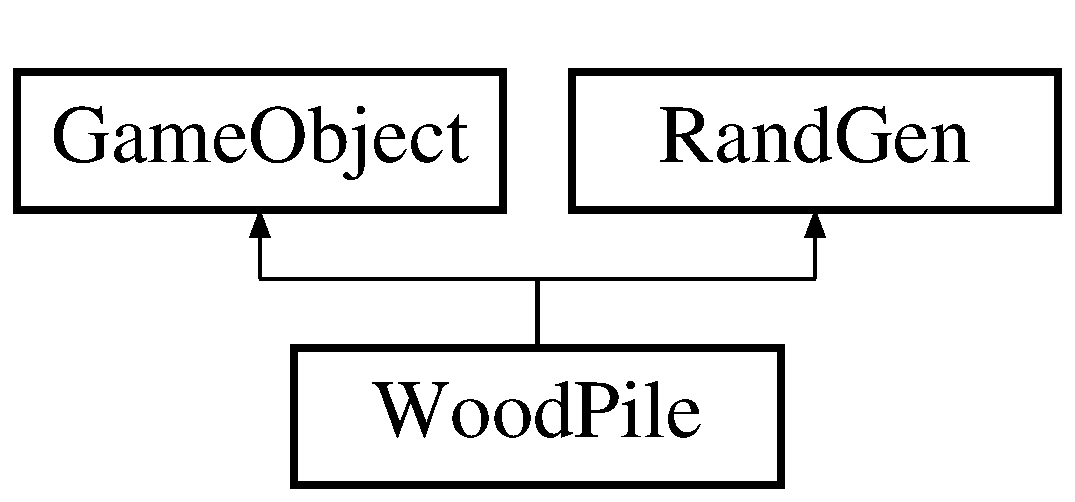
\includegraphics[height=2.000000cm]{class_wood_pile}
\end{center}
\end{figure}
\subsection*{Public Member Functions}
\begin{DoxyCompactItemize}
\item 
\mbox{\hyperlink{class_wood_pile_a9572061fc6db784b5acc68cde0c95435}{Wood\+Pile}} ()
\item 
\mbox{\hyperlink{class_wood_pile_a7bce94d6dd074921d7905d300f5cb82a}{$\sim$\+Wood\+Pile}} ()
\item 
void \mbox{\hyperlink{class_wood_pile_a19156e17630117c4e031ccd594101d1a}{m\+\_\+\+Init\+Wood\+Pile}} (\mbox{\hyperlink{class_cells}{Cells}} $\ast$pile\+Location, sf\+::\+Font new\+Font, float current\+Growth)
\item 
void \mbox{\hyperlink{class_wood_pile_a32821c728e54c6c77c922e3c5a4d1cb8}{m\+\_\+\+Assign\+Texture}} (sf\+::\+Texture new\+Texture)
\item 
void \mbox{\hyperlink{class_wood_pile_a008e8dc7b168ab4e0bcc946c240d0a32}{m\+\_\+\+Update}} ()
\item 
int \mbox{\hyperlink{class_wood_pile_ae034c119180b63f716472739b80f9f63}{m\+\_\+\+Take\+Wood}} (int amount\+Taken)
\item 
bool \mbox{\hyperlink{class_wood_pile_aa0e4d61a9d9b42b4ec4b0f129f6b60d6}{m\+\_\+\+Get\+Mark\+For\+Deletion}} ()
\item 
void \mbox{\hyperlink{class_wood_pile_aacdd6153eacdeaf06cddf83cca50da03}{m\+\_\+\+Draw\+Game\+Object}} (sf\+::\+Render\+Window \&window)
\item 
void \mbox{\hyperlink{class_wood_pile_a4434a4c1251a6719b76825a7546ca04c}{m\+\_\+\+Draw\+Filter}} (sf\+::\+Vector2f top\+Left, sf\+::\+Vector2f bottom\+Right)
\item 
void \mbox{\hyperlink{class_wood_pile_a813fd022f48917ee10b81c94810d27ad}{m\+\_\+\+Draw\+Filter}} (sf\+::\+Vector2f top\+Left, sf\+::\+Vector2f bottom\+Right, int current\+Layer)
\item 
void \mbox{\hyperlink{class_wood_pile_a8faa580584607dea772076b7d856daf8}{m\+\_\+\+Set\+Object\+Pos}} (float x, float y)
\item 
\mbox{\hyperlink{class_cells}{Cells}} $\ast$ \mbox{\hyperlink{class_wood_pile_ac5f5d04824b12b5e31ffe1d4ba92dbf5}{m\+\_\+\+Get\+Curent\+Cell}} ()
\end{DoxyCompactItemize}
\subsection*{Additional Inherited Members}


\subsection{Constructor \& Destructor Documentation}
\mbox{\Hypertarget{class_wood_pile_a9572061fc6db784b5acc68cde0c95435}\label{class_wood_pile_a9572061fc6db784b5acc68cde0c95435}} 
\index{Wood\+Pile@{Wood\+Pile}!Wood\+Pile@{Wood\+Pile}}
\index{Wood\+Pile@{Wood\+Pile}!Wood\+Pile@{Wood\+Pile}}
\subsubsection{\texorpdfstring{Wood\+Pile()}{WoodPile()}}
{\footnotesize\ttfamily Wood\+Pile\+::\+Wood\+Pile (\begin{DoxyParamCaption}{ }\end{DoxyParamCaption})}

\mbox{\Hypertarget{class_wood_pile_a7bce94d6dd074921d7905d300f5cb82a}\label{class_wood_pile_a7bce94d6dd074921d7905d300f5cb82a}} 
\index{Wood\+Pile@{Wood\+Pile}!````~Wood\+Pile@{$\sim$\+Wood\+Pile}}
\index{````~Wood\+Pile@{$\sim$\+Wood\+Pile}!Wood\+Pile@{Wood\+Pile}}
\subsubsection{\texorpdfstring{$\sim$\+Wood\+Pile()}{~WoodPile()}}
{\footnotesize\ttfamily Wood\+Pile\+::$\sim$\+Wood\+Pile (\begin{DoxyParamCaption}{ }\end{DoxyParamCaption})}



\subsection{Member Function Documentation}
\mbox{\Hypertarget{class_wood_pile_a32821c728e54c6c77c922e3c5a4d1cb8}\label{class_wood_pile_a32821c728e54c6c77c922e3c5a4d1cb8}} 
\index{Wood\+Pile@{Wood\+Pile}!m\+\_\+\+Assign\+Texture@{m\+\_\+\+Assign\+Texture}}
\index{m\+\_\+\+Assign\+Texture@{m\+\_\+\+Assign\+Texture}!Wood\+Pile@{Wood\+Pile}}
\subsubsection{\texorpdfstring{m\+\_\+\+Assign\+Texture()}{m\_AssignTexture()}}
{\footnotesize\ttfamily void Wood\+Pile\+::m\+\_\+\+Assign\+Texture (\begin{DoxyParamCaption}\item[{sf\+::\+Texture}]{new\+Texture }\end{DoxyParamCaption})}

\mbox{\Hypertarget{class_wood_pile_a4434a4c1251a6719b76825a7546ca04c}\label{class_wood_pile_a4434a4c1251a6719b76825a7546ca04c}} 
\index{Wood\+Pile@{Wood\+Pile}!m\+\_\+\+Draw\+Filter@{m\+\_\+\+Draw\+Filter}}
\index{m\+\_\+\+Draw\+Filter@{m\+\_\+\+Draw\+Filter}!Wood\+Pile@{Wood\+Pile}}
\subsubsection{\texorpdfstring{m\+\_\+\+Draw\+Filter()}{m\_DrawFilter()}\hspace{0.1cm}{\footnotesize\ttfamily [1/2]}}
{\footnotesize\ttfamily void Wood\+Pile\+::m\+\_\+\+Draw\+Filter (\begin{DoxyParamCaption}\item[{sf\+::\+Vector2f}]{top\+Left,  }\item[{sf\+::\+Vector2f}]{bottom\+Right }\end{DoxyParamCaption})\hspace{0.3cm}{\ttfamily [virtual]}}



Implements \mbox{\hyperlink{class_game_object_af1a0662ca445d878b163c4648f90259c}{Game\+Object}}.

\mbox{\Hypertarget{class_wood_pile_a813fd022f48917ee10b81c94810d27ad}\label{class_wood_pile_a813fd022f48917ee10b81c94810d27ad}} 
\index{Wood\+Pile@{Wood\+Pile}!m\+\_\+\+Draw\+Filter@{m\+\_\+\+Draw\+Filter}}
\index{m\+\_\+\+Draw\+Filter@{m\+\_\+\+Draw\+Filter}!Wood\+Pile@{Wood\+Pile}}
\subsubsection{\texorpdfstring{m\+\_\+\+Draw\+Filter()}{m\_DrawFilter()}\hspace{0.1cm}{\footnotesize\ttfamily [2/2]}}
{\footnotesize\ttfamily void Wood\+Pile\+::m\+\_\+\+Draw\+Filter (\begin{DoxyParamCaption}\item[{sf\+::\+Vector2f}]{top\+Left,  }\item[{sf\+::\+Vector2f}]{bottom\+Right,  }\item[{int}]{current\+Layer }\end{DoxyParamCaption})}

\mbox{\Hypertarget{class_wood_pile_aacdd6153eacdeaf06cddf83cca50da03}\label{class_wood_pile_aacdd6153eacdeaf06cddf83cca50da03}} 
\index{Wood\+Pile@{Wood\+Pile}!m\+\_\+\+Draw\+Game\+Object@{m\+\_\+\+Draw\+Game\+Object}}
\index{m\+\_\+\+Draw\+Game\+Object@{m\+\_\+\+Draw\+Game\+Object}!Wood\+Pile@{Wood\+Pile}}
\subsubsection{\texorpdfstring{m\+\_\+\+Draw\+Game\+Object()}{m\_DrawGameObject()}}
{\footnotesize\ttfamily void Wood\+Pile\+::m\+\_\+\+Draw\+Game\+Object (\begin{DoxyParamCaption}\item[{sf\+::\+Render\+Window \&}]{window }\end{DoxyParamCaption})\hspace{0.3cm}{\ttfamily [virtual]}}



Implements \mbox{\hyperlink{class_game_object_a184ac59fd5167c55a54b50894e5b6721}{Game\+Object}}.

\mbox{\Hypertarget{class_wood_pile_ac5f5d04824b12b5e31ffe1d4ba92dbf5}\label{class_wood_pile_ac5f5d04824b12b5e31ffe1d4ba92dbf5}} 
\index{Wood\+Pile@{Wood\+Pile}!m\+\_\+\+Get\+Curent\+Cell@{m\+\_\+\+Get\+Curent\+Cell}}
\index{m\+\_\+\+Get\+Curent\+Cell@{m\+\_\+\+Get\+Curent\+Cell}!Wood\+Pile@{Wood\+Pile}}
\subsubsection{\texorpdfstring{m\+\_\+\+Get\+Curent\+Cell()}{m\_GetCurentCell()}}
{\footnotesize\ttfamily \mbox{\hyperlink{class_cells}{Cells}}$\ast$ Wood\+Pile\+::m\+\_\+\+Get\+Curent\+Cell (\begin{DoxyParamCaption}{ }\end{DoxyParamCaption})}

\mbox{\Hypertarget{class_wood_pile_aa0e4d61a9d9b42b4ec4b0f129f6b60d6}\label{class_wood_pile_aa0e4d61a9d9b42b4ec4b0f129f6b60d6}} 
\index{Wood\+Pile@{Wood\+Pile}!m\+\_\+\+Get\+Mark\+For\+Deletion@{m\+\_\+\+Get\+Mark\+For\+Deletion}}
\index{m\+\_\+\+Get\+Mark\+For\+Deletion@{m\+\_\+\+Get\+Mark\+For\+Deletion}!Wood\+Pile@{Wood\+Pile}}
\subsubsection{\texorpdfstring{m\+\_\+\+Get\+Mark\+For\+Deletion()}{m\_GetMarkForDeletion()}}
{\footnotesize\ttfamily bool Wood\+Pile\+::m\+\_\+\+Get\+Mark\+For\+Deletion (\begin{DoxyParamCaption}{ }\end{DoxyParamCaption})}

\mbox{\Hypertarget{class_wood_pile_a19156e17630117c4e031ccd594101d1a}\label{class_wood_pile_a19156e17630117c4e031ccd594101d1a}} 
\index{Wood\+Pile@{Wood\+Pile}!m\+\_\+\+Init\+Wood\+Pile@{m\+\_\+\+Init\+Wood\+Pile}}
\index{m\+\_\+\+Init\+Wood\+Pile@{m\+\_\+\+Init\+Wood\+Pile}!Wood\+Pile@{Wood\+Pile}}
\subsubsection{\texorpdfstring{m\+\_\+\+Init\+Wood\+Pile()}{m\_InitWoodPile()}}
{\footnotesize\ttfamily void Wood\+Pile\+::m\+\_\+\+Init\+Wood\+Pile (\begin{DoxyParamCaption}\item[{\mbox{\hyperlink{class_cells}{Cells}} $\ast$}]{pile\+Location,  }\item[{sf\+::\+Font}]{new\+Font,  }\item[{float}]{current\+Growth }\end{DoxyParamCaption})}

\mbox{\Hypertarget{class_wood_pile_a8faa580584607dea772076b7d856daf8}\label{class_wood_pile_a8faa580584607dea772076b7d856daf8}} 
\index{Wood\+Pile@{Wood\+Pile}!m\+\_\+\+Set\+Object\+Pos@{m\+\_\+\+Set\+Object\+Pos}}
\index{m\+\_\+\+Set\+Object\+Pos@{m\+\_\+\+Set\+Object\+Pos}!Wood\+Pile@{Wood\+Pile}}
\subsubsection{\texorpdfstring{m\+\_\+\+Set\+Object\+Pos()}{m\_SetObjectPos()}}
{\footnotesize\ttfamily void Wood\+Pile\+::m\+\_\+\+Set\+Object\+Pos (\begin{DoxyParamCaption}\item[{float}]{x,  }\item[{float}]{y }\end{DoxyParamCaption})\hspace{0.3cm}{\ttfamily [virtual]}}



Implements \mbox{\hyperlink{class_game_object_ad1f8ea8eb3673b1af8215bf92cdc0df8}{Game\+Object}}.

\mbox{\Hypertarget{class_wood_pile_ae034c119180b63f716472739b80f9f63}\label{class_wood_pile_ae034c119180b63f716472739b80f9f63}} 
\index{Wood\+Pile@{Wood\+Pile}!m\+\_\+\+Take\+Wood@{m\+\_\+\+Take\+Wood}}
\index{m\+\_\+\+Take\+Wood@{m\+\_\+\+Take\+Wood}!Wood\+Pile@{Wood\+Pile}}
\subsubsection{\texorpdfstring{m\+\_\+\+Take\+Wood()}{m\_TakeWood()}}
{\footnotesize\ttfamily int Wood\+Pile\+::m\+\_\+\+Take\+Wood (\begin{DoxyParamCaption}\item[{int}]{amount\+Taken }\end{DoxyParamCaption})}

\mbox{\Hypertarget{class_wood_pile_a008e8dc7b168ab4e0bcc946c240d0a32}\label{class_wood_pile_a008e8dc7b168ab4e0bcc946c240d0a32}} 
\index{Wood\+Pile@{Wood\+Pile}!m\+\_\+\+Update@{m\+\_\+\+Update}}
\index{m\+\_\+\+Update@{m\+\_\+\+Update}!Wood\+Pile@{Wood\+Pile}}
\subsubsection{\texorpdfstring{m\+\_\+\+Update()}{m\_Update()}}
{\footnotesize\ttfamily void Wood\+Pile\+::m\+\_\+\+Update (\begin{DoxyParamCaption}{ }\end{DoxyParamCaption})\hspace{0.3cm}{\ttfamily [virtual]}}



Implements \mbox{\hyperlink{class_game_object_a3af5a7b470e09f13a1422439fc6a9ba8}{Game\+Object}}.



The documentation for this class was generated from the following file\+:\begin{DoxyCompactItemize}
\item 
inc/\mbox{\hyperlink{_wood_pile_8h}{Wood\+Pile.\+h}}\end{DoxyCompactItemize}

\hypertarget{class_wood_resource}{}\section{Wood\+Resource Class Reference}
\label{class_wood_resource}\index{Wood\+Resource@{Wood\+Resource}}


{\ttfamily \#include $<$Wood\+Resource.\+h$>$}

Inheritance diagram for Wood\+Resource\+:\begin{figure}[H]
\begin{center}
\leavevmode
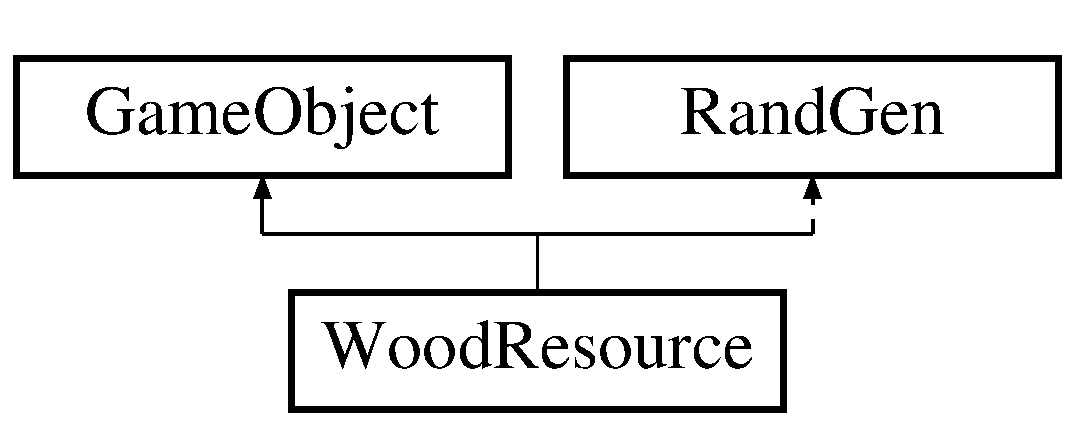
\includegraphics[height=2.000000cm]{class_wood_resource}
\end{center}
\end{figure}
\subsection*{Public Member Functions}
\begin{DoxyCompactItemize}
\item 
\mbox{\hyperlink{class_wood_resource_a692782e93b0450b26694eb3d48c86a2a}{Wood\+Resource}} ()
\item 
\mbox{\hyperlink{class_wood_resource_ad525b51c0f4728951969b90498760a63}{$\sim$\+Wood\+Resource}} ()
\item 
void \mbox{\hyperlink{class_wood_resource_aeea45c6a211c4662ff114cd77f604c68}{m\+\_\+\+Create\+Tree}} (float radius, sf\+::\+Vector2f position, int layer, \mbox{\hyperlink{class_cells}{Cells}} $\ast$new\+Current\+Cell)
\item 
void \mbox{\hyperlink{class_wood_resource_a8ba1b597aacbdd74be37d0ab18d95008}{m\+\_\+\+Update}} () override
\item 
void \mbox{\hyperlink{class_wood_resource_a8f2336619be4467ba0eba87ded7b7474}{m\+\_\+\+Draw\+Game\+Object}} (sf\+::\+Render\+Window \&window) override
\item 
void \mbox{\hyperlink{class_wood_resource_a08e9ac9417b6337b4fe8afcb97783acf}{m\+\_\+\+Draw\+Filter}} (sf\+::\+Vector2f top\+Left, sf\+::\+Vector2f bottom\+Right) override
\item 
void \mbox{\hyperlink{class_wood_resource_acdbde685c1d8f702b41d89763f7bb0c7}{m\+\_\+\+Draw\+Filter}} (sf\+::\+Vector2f top\+Left, sf\+::\+Vector2f bottom\+Right, int current\+Layer)
\item 
void \mbox{\hyperlink{class_wood_resource_afa9f748e3dea5f08c18dd831f04d9287}{m\+\_\+\+Set\+Object\+Pos}} (float x, float y) override
\item 
\mbox{\hyperlink{class_cells}{Cells}} $\ast$ \mbox{\hyperlink{class_wood_resource_a9c7446775e6e37e60a0bfce147d8151f}{m\+\_\+\+Get\+Current\+Cell}} ()
\item 
void \mbox{\hyperlink{class_wood_resource_a90aadace134336f71aed1c167983c711}{m\+\_\+\+Set\+Tree\+Cut\+Down}} ()
\item 
void \mbox{\hyperlink{class_wood_resource_a5006853189de66810cbbfb2500b559c0}{m\+\_\+\+Set\+Mark\+For\+Deletion}} (bool remove\+This)
\item 
bool \mbox{\hyperlink{class_wood_resource_ac63bf6a2a12aed793b4e1da4aae57c00}{m\+\_\+\+Get\+Mark\+For\+Deletion}} ()
\item 
float \mbox{\hyperlink{class_wood_resource_a185e4bc651ee95a51239d8842c9c3773}{m\+\_\+\+Get\+Current\+Growth}} ()
\item 
void \mbox{\hyperlink{class_wood_resource_ab0aabdbb9fc8c1ff574a8528b6cda537}{m\+\_\+\+Cancel\+Tree\+Cut\+Down}} ()
\item 
bool \mbox{\hyperlink{class_wood_resource_aa7228add3ddade14e54acc5647b79a14}{m\+\_\+\+Get\+Tree\+Cut\+Down}} ()
\end{DoxyCompactItemize}
\subsection*{Additional Inherited Members}


\subsection{Constructor \& Destructor Documentation}
\mbox{\Hypertarget{class_wood_resource_a692782e93b0450b26694eb3d48c86a2a}\label{class_wood_resource_a692782e93b0450b26694eb3d48c86a2a}} 
\index{Wood\+Resource@{Wood\+Resource}!Wood\+Resource@{Wood\+Resource}}
\index{Wood\+Resource@{Wood\+Resource}!Wood\+Resource@{Wood\+Resource}}
\subsubsection{\texorpdfstring{Wood\+Resource()}{WoodResource()}}
{\footnotesize\ttfamily Wood\+Resource\+::\+Wood\+Resource (\begin{DoxyParamCaption}{ }\end{DoxyParamCaption})}

\mbox{\Hypertarget{class_wood_resource_ad525b51c0f4728951969b90498760a63}\label{class_wood_resource_ad525b51c0f4728951969b90498760a63}} 
\index{Wood\+Resource@{Wood\+Resource}!````~Wood\+Resource@{$\sim$\+Wood\+Resource}}
\index{````~Wood\+Resource@{$\sim$\+Wood\+Resource}!Wood\+Resource@{Wood\+Resource}}
\subsubsection{\texorpdfstring{$\sim$\+Wood\+Resource()}{~WoodResource()}}
{\footnotesize\ttfamily Wood\+Resource\+::$\sim$\+Wood\+Resource (\begin{DoxyParamCaption}{ }\end{DoxyParamCaption})}



\subsection{Member Function Documentation}
\mbox{\Hypertarget{class_wood_resource_ab0aabdbb9fc8c1ff574a8528b6cda537}\label{class_wood_resource_ab0aabdbb9fc8c1ff574a8528b6cda537}} 
\index{Wood\+Resource@{Wood\+Resource}!m\+\_\+\+Cancel\+Tree\+Cut\+Down@{m\+\_\+\+Cancel\+Tree\+Cut\+Down}}
\index{m\+\_\+\+Cancel\+Tree\+Cut\+Down@{m\+\_\+\+Cancel\+Tree\+Cut\+Down}!Wood\+Resource@{Wood\+Resource}}
\subsubsection{\texorpdfstring{m\+\_\+\+Cancel\+Tree\+Cut\+Down()}{m\_CancelTreeCutDown()}}
{\footnotesize\ttfamily void Wood\+Resource\+::m\+\_\+\+Cancel\+Tree\+Cut\+Down (\begin{DoxyParamCaption}{ }\end{DoxyParamCaption})}

\mbox{\Hypertarget{class_wood_resource_aeea45c6a211c4662ff114cd77f604c68}\label{class_wood_resource_aeea45c6a211c4662ff114cd77f604c68}} 
\index{Wood\+Resource@{Wood\+Resource}!m\+\_\+\+Create\+Tree@{m\+\_\+\+Create\+Tree}}
\index{m\+\_\+\+Create\+Tree@{m\+\_\+\+Create\+Tree}!Wood\+Resource@{Wood\+Resource}}
\subsubsection{\texorpdfstring{m\+\_\+\+Create\+Tree()}{m\_CreateTree()}}
{\footnotesize\ttfamily void Wood\+Resource\+::m\+\_\+\+Create\+Tree (\begin{DoxyParamCaption}\item[{float}]{radius,  }\item[{sf\+::\+Vector2f}]{position,  }\item[{int}]{layer,  }\item[{\mbox{\hyperlink{class_cells}{Cells}} $\ast$}]{new\+Current\+Cell }\end{DoxyParamCaption})}

\mbox{\Hypertarget{class_wood_resource_a08e9ac9417b6337b4fe8afcb97783acf}\label{class_wood_resource_a08e9ac9417b6337b4fe8afcb97783acf}} 
\index{Wood\+Resource@{Wood\+Resource}!m\+\_\+\+Draw\+Filter@{m\+\_\+\+Draw\+Filter}}
\index{m\+\_\+\+Draw\+Filter@{m\+\_\+\+Draw\+Filter}!Wood\+Resource@{Wood\+Resource}}
\subsubsection{\texorpdfstring{m\+\_\+\+Draw\+Filter()}{m\_DrawFilter()}\hspace{0.1cm}{\footnotesize\ttfamily [1/2]}}
{\footnotesize\ttfamily void Wood\+Resource\+::m\+\_\+\+Draw\+Filter (\begin{DoxyParamCaption}\item[{sf\+::\+Vector2f}]{top\+Left,  }\item[{sf\+::\+Vector2f}]{bottom\+Right }\end{DoxyParamCaption})\hspace{0.3cm}{\ttfamily [override]}, {\ttfamily [virtual]}}



Implements \mbox{\hyperlink{class_game_object_af1a0662ca445d878b163c4648f90259c}{Game\+Object}}.

\mbox{\Hypertarget{class_wood_resource_acdbde685c1d8f702b41d89763f7bb0c7}\label{class_wood_resource_acdbde685c1d8f702b41d89763f7bb0c7}} 
\index{Wood\+Resource@{Wood\+Resource}!m\+\_\+\+Draw\+Filter@{m\+\_\+\+Draw\+Filter}}
\index{m\+\_\+\+Draw\+Filter@{m\+\_\+\+Draw\+Filter}!Wood\+Resource@{Wood\+Resource}}
\subsubsection{\texorpdfstring{m\+\_\+\+Draw\+Filter()}{m\_DrawFilter()}\hspace{0.1cm}{\footnotesize\ttfamily [2/2]}}
{\footnotesize\ttfamily void Wood\+Resource\+::m\+\_\+\+Draw\+Filter (\begin{DoxyParamCaption}\item[{sf\+::\+Vector2f}]{top\+Left,  }\item[{sf\+::\+Vector2f}]{bottom\+Right,  }\item[{int}]{current\+Layer }\end{DoxyParamCaption})}

\mbox{\Hypertarget{class_wood_resource_a8f2336619be4467ba0eba87ded7b7474}\label{class_wood_resource_a8f2336619be4467ba0eba87ded7b7474}} 
\index{Wood\+Resource@{Wood\+Resource}!m\+\_\+\+Draw\+Game\+Object@{m\+\_\+\+Draw\+Game\+Object}}
\index{m\+\_\+\+Draw\+Game\+Object@{m\+\_\+\+Draw\+Game\+Object}!Wood\+Resource@{Wood\+Resource}}
\subsubsection{\texorpdfstring{m\+\_\+\+Draw\+Game\+Object()}{m\_DrawGameObject()}}
{\footnotesize\ttfamily void Wood\+Resource\+::m\+\_\+\+Draw\+Game\+Object (\begin{DoxyParamCaption}\item[{sf\+::\+Render\+Window \&}]{window }\end{DoxyParamCaption})\hspace{0.3cm}{\ttfamily [override]}, {\ttfamily [virtual]}}



Implements \mbox{\hyperlink{class_game_object_a184ac59fd5167c55a54b50894e5b6721}{Game\+Object}}.

\mbox{\Hypertarget{class_wood_resource_a9c7446775e6e37e60a0bfce147d8151f}\label{class_wood_resource_a9c7446775e6e37e60a0bfce147d8151f}} 
\index{Wood\+Resource@{Wood\+Resource}!m\+\_\+\+Get\+Current\+Cell@{m\+\_\+\+Get\+Current\+Cell}}
\index{m\+\_\+\+Get\+Current\+Cell@{m\+\_\+\+Get\+Current\+Cell}!Wood\+Resource@{Wood\+Resource}}
\subsubsection{\texorpdfstring{m\+\_\+\+Get\+Current\+Cell()}{m\_GetCurrentCell()}}
{\footnotesize\ttfamily \mbox{\hyperlink{class_cells}{Cells}}$\ast$ Wood\+Resource\+::m\+\_\+\+Get\+Current\+Cell (\begin{DoxyParamCaption}{ }\end{DoxyParamCaption})}

\mbox{\Hypertarget{class_wood_resource_a185e4bc651ee95a51239d8842c9c3773}\label{class_wood_resource_a185e4bc651ee95a51239d8842c9c3773}} 
\index{Wood\+Resource@{Wood\+Resource}!m\+\_\+\+Get\+Current\+Growth@{m\+\_\+\+Get\+Current\+Growth}}
\index{m\+\_\+\+Get\+Current\+Growth@{m\+\_\+\+Get\+Current\+Growth}!Wood\+Resource@{Wood\+Resource}}
\subsubsection{\texorpdfstring{m\+\_\+\+Get\+Current\+Growth()}{m\_GetCurrentGrowth()}}
{\footnotesize\ttfamily float Wood\+Resource\+::m\+\_\+\+Get\+Current\+Growth (\begin{DoxyParamCaption}{ }\end{DoxyParamCaption})}

\mbox{\Hypertarget{class_wood_resource_ac63bf6a2a12aed793b4e1da4aae57c00}\label{class_wood_resource_ac63bf6a2a12aed793b4e1da4aae57c00}} 
\index{Wood\+Resource@{Wood\+Resource}!m\+\_\+\+Get\+Mark\+For\+Deletion@{m\+\_\+\+Get\+Mark\+For\+Deletion}}
\index{m\+\_\+\+Get\+Mark\+For\+Deletion@{m\+\_\+\+Get\+Mark\+For\+Deletion}!Wood\+Resource@{Wood\+Resource}}
\subsubsection{\texorpdfstring{m\+\_\+\+Get\+Mark\+For\+Deletion()}{m\_GetMarkForDeletion()}}
{\footnotesize\ttfamily bool Wood\+Resource\+::m\+\_\+\+Get\+Mark\+For\+Deletion (\begin{DoxyParamCaption}{ }\end{DoxyParamCaption})}

\mbox{\Hypertarget{class_wood_resource_aa7228add3ddade14e54acc5647b79a14}\label{class_wood_resource_aa7228add3ddade14e54acc5647b79a14}} 
\index{Wood\+Resource@{Wood\+Resource}!m\+\_\+\+Get\+Tree\+Cut\+Down@{m\+\_\+\+Get\+Tree\+Cut\+Down}}
\index{m\+\_\+\+Get\+Tree\+Cut\+Down@{m\+\_\+\+Get\+Tree\+Cut\+Down}!Wood\+Resource@{Wood\+Resource}}
\subsubsection{\texorpdfstring{m\+\_\+\+Get\+Tree\+Cut\+Down()}{m\_GetTreeCutDown()}}
{\footnotesize\ttfamily bool Wood\+Resource\+::m\+\_\+\+Get\+Tree\+Cut\+Down (\begin{DoxyParamCaption}{ }\end{DoxyParamCaption})}

\mbox{\Hypertarget{class_wood_resource_a5006853189de66810cbbfb2500b559c0}\label{class_wood_resource_a5006853189de66810cbbfb2500b559c0}} 
\index{Wood\+Resource@{Wood\+Resource}!m\+\_\+\+Set\+Mark\+For\+Deletion@{m\+\_\+\+Set\+Mark\+For\+Deletion}}
\index{m\+\_\+\+Set\+Mark\+For\+Deletion@{m\+\_\+\+Set\+Mark\+For\+Deletion}!Wood\+Resource@{Wood\+Resource}}
\subsubsection{\texorpdfstring{m\+\_\+\+Set\+Mark\+For\+Deletion()}{m\_SetMarkForDeletion()}}
{\footnotesize\ttfamily void Wood\+Resource\+::m\+\_\+\+Set\+Mark\+For\+Deletion (\begin{DoxyParamCaption}\item[{bool}]{remove\+This }\end{DoxyParamCaption})}

\mbox{\Hypertarget{class_wood_resource_afa9f748e3dea5f08c18dd831f04d9287}\label{class_wood_resource_afa9f748e3dea5f08c18dd831f04d9287}} 
\index{Wood\+Resource@{Wood\+Resource}!m\+\_\+\+Set\+Object\+Pos@{m\+\_\+\+Set\+Object\+Pos}}
\index{m\+\_\+\+Set\+Object\+Pos@{m\+\_\+\+Set\+Object\+Pos}!Wood\+Resource@{Wood\+Resource}}
\subsubsection{\texorpdfstring{m\+\_\+\+Set\+Object\+Pos()}{m\_SetObjectPos()}}
{\footnotesize\ttfamily void Wood\+Resource\+::m\+\_\+\+Set\+Object\+Pos (\begin{DoxyParamCaption}\item[{float}]{x,  }\item[{float}]{y }\end{DoxyParamCaption})\hspace{0.3cm}{\ttfamily [override]}, {\ttfamily [virtual]}}



Implements \mbox{\hyperlink{class_game_object_ad1f8ea8eb3673b1af8215bf92cdc0df8}{Game\+Object}}.

\mbox{\Hypertarget{class_wood_resource_a90aadace134336f71aed1c167983c711}\label{class_wood_resource_a90aadace134336f71aed1c167983c711}} 
\index{Wood\+Resource@{Wood\+Resource}!m\+\_\+\+Set\+Tree\+Cut\+Down@{m\+\_\+\+Set\+Tree\+Cut\+Down}}
\index{m\+\_\+\+Set\+Tree\+Cut\+Down@{m\+\_\+\+Set\+Tree\+Cut\+Down}!Wood\+Resource@{Wood\+Resource}}
\subsubsection{\texorpdfstring{m\+\_\+\+Set\+Tree\+Cut\+Down()}{m\_SetTreeCutDown()}}
{\footnotesize\ttfamily void Wood\+Resource\+::m\+\_\+\+Set\+Tree\+Cut\+Down (\begin{DoxyParamCaption}{ }\end{DoxyParamCaption})}

\mbox{\Hypertarget{class_wood_resource_a8ba1b597aacbdd74be37d0ab18d95008}\label{class_wood_resource_a8ba1b597aacbdd74be37d0ab18d95008}} 
\index{Wood\+Resource@{Wood\+Resource}!m\+\_\+\+Update@{m\+\_\+\+Update}}
\index{m\+\_\+\+Update@{m\+\_\+\+Update}!Wood\+Resource@{Wood\+Resource}}
\subsubsection{\texorpdfstring{m\+\_\+\+Update()}{m\_Update()}}
{\footnotesize\ttfamily void Wood\+Resource\+::m\+\_\+\+Update (\begin{DoxyParamCaption}{ }\end{DoxyParamCaption})\hspace{0.3cm}{\ttfamily [override]}, {\ttfamily [virtual]}}



Implements \mbox{\hyperlink{class_game_object_a3af5a7b470e09f13a1422439fc6a9ba8}{Game\+Object}}.



The documentation for this class was generated from the following file\+:\begin{DoxyCompactItemize}
\item 
inc/\mbox{\hyperlink{_wood_resource_8h}{Wood\+Resource.\+h}}\end{DoxyCompactItemize}

\chapter{File Documentation}
\hypertarget{_building_manager_8h}{}\section{inc/\+Building\+Manager.h File Reference}
\label{_building_manager_8h}\index{inc/\+Building\+Manager.\+h@{inc/\+Building\+Manager.\+h}}
{\ttfamily \#include \char`\"{}defs.\+h\char`\"{}}\newline
{\ttfamily \#include \char`\"{}Building\+Object.\+h\char`\"{}}\newline
\subsection*{Classes}
\begin{DoxyCompactItemize}
\item 
class \mbox{\hyperlink{class_building_manager}{Building\+Manager}}
\end{DoxyCompactItemize}

\hypertarget{_building_object_8h}{}\section{inc/\+Building\+Object.h File Reference}
\label{_building_object_8h}\index{inc/\+Building\+Object.\+h@{inc/\+Building\+Object.\+h}}
{\ttfamily \#include \char`\"{}defs.\+h\char`\"{}}\newline
{\ttfamily \#include \char`\"{}Game\+Object.\+h\char`\"{}}\newline
{\ttfamily \#include \char`\"{}Cells.\+h\char`\"{}}\newline
\subsection*{Classes}
\begin{DoxyCompactItemize}
\item 
class \mbox{\hyperlink{class_building_object}{Building\+Object}}
\end{DoxyCompactItemize}

\hypertarget{_cells_8h}{}\section{inc/\+Cells.h File Reference}
\label{_cells_8h}\index{inc/\+Cells.\+h@{inc/\+Cells.\+h}}
{\ttfamily \#include \char`\"{}defs.\+h\char`\"{}}\newline
{\ttfamily \#include \char`\"{}Game\+Object.\+h\char`\"{}}\newline
\subsection*{Classes}
\begin{DoxyCompactItemize}
\item 
struct \mbox{\hyperlink{structgrid_pos}{grid\+Pos}}
\item 
class \mbox{\hyperlink{class_cells}{Cells}}
\end{DoxyCompactItemize}
\subsection*{Enumerations}
\begin{DoxyCompactItemize}
\item 
enum \mbox{\hyperlink{_cells_8h_adc5e4636eae42cdad2a070c6adbd9daf}{tile\+Set}} \{ \newline
\mbox{\hyperlink{_cells_8h_adc5e4636eae42cdad2a070c6adbd9dafadb74a8405410b3dfcb151d7de961197e}{\+\_\+\+D\+I\+RT}} = 0x2000, 
\mbox{\hyperlink{_cells_8h_adc5e4636eae42cdad2a070c6adbd9dafa2d9029edab7daff377235047ef34bc85}{\+\_\+\+W\+A\+T\+ER}} = 0x3000, 
\mbox{\hyperlink{_cells_8h_adc5e4636eae42cdad2a070c6adbd9dafa0a58ab7f51305b66af577ff8f036bfc8}{\+\_\+\+R\+O\+CK}} = 0x4000, 
\mbox{\hyperlink{_cells_8h_adc5e4636eae42cdad2a070c6adbd9dafa841c1e89d9531a64c778491c4311c46c}{\+\_\+\+S\+KY}} = 0x5000, 
\newline
\mbox{\hyperlink{_cells_8h_adc5e4636eae42cdad2a070c6adbd9dafa64fe0db38eba54ba41835d7370c0d4b6}{\+\_\+\+N\+O\+\_\+\+V\+A\+L\+UE}}
 \}
\item 
enum \mbox{\hyperlink{_cells_8h_a7ba65324a33605edc81596f69733023a}{huristic\+Cost}} \{ \mbox{\hyperlink{_cells_8h_a7ba65324a33605edc81596f69733023aaed3a8b9863389cd8176ae6b75f58341c}{\+\_\+\+D\+I\+A\+G\+O\+N\+AL}} = 14, 
\mbox{\hyperlink{_cells_8h_a7ba65324a33605edc81596f69733023aa9c824b9ad88177834284219918f2025d}{\+\_\+\+A\+C\+R\+O\+SS}} = 10
 \}
\end{DoxyCompactItemize}


\subsection{Detailed Description}
\mbox{\hyperlink{class_this}{This}} will hold the information for a single cell within the game. A group of cells will form a either a row or a column. 

\subsection{Enumeration Type Documentation}
\mbox{\Hypertarget{_cells_8h_a7ba65324a33605edc81596f69733023a}\label{_cells_8h_a7ba65324a33605edc81596f69733023a}} 
\index{Cells.\+h@{Cells.\+h}!huristic\+Cost@{huristic\+Cost}}
\index{huristic\+Cost@{huristic\+Cost}!Cells.\+h@{Cells.\+h}}
\subsubsection{\texorpdfstring{huristic\+Cost}{huristicCost}}
{\footnotesize\ttfamily enum \mbox{\hyperlink{_cells_8h_a7ba65324a33605edc81596f69733023a}{huristic\+Cost}}}

\begin{DoxyEnumFields}{Enumerator}
\raisebox{\heightof{T}}[0pt][0pt]{\index{\+\_\+\+D\+I\+A\+G\+O\+N\+AL@{\+\_\+\+D\+I\+A\+G\+O\+N\+AL}!Cells.\+h@{Cells.\+h}}\index{Cells.\+h@{Cells.\+h}!\+\_\+\+D\+I\+A\+G\+O\+N\+AL@{\+\_\+\+D\+I\+A\+G\+O\+N\+AL}}}\mbox{\Hypertarget{_cells_8h_a7ba65324a33605edc81596f69733023aaed3a8b9863389cd8176ae6b75f58341c}\label{_cells_8h_a7ba65324a33605edc81596f69733023aaed3a8b9863389cd8176ae6b75f58341c}} 
\+\_\+\+D\+I\+A\+G\+O\+N\+AL&The cost of moving diagonally in A$\ast$. \\
\hline

\raisebox{\heightof{T}}[0pt][0pt]{\index{\+\_\+\+A\+C\+R\+O\+SS@{\+\_\+\+A\+C\+R\+O\+SS}!Cells.\+h@{Cells.\+h}}\index{Cells.\+h@{Cells.\+h}!\+\_\+\+A\+C\+R\+O\+SS@{\+\_\+\+A\+C\+R\+O\+SS}}}\mbox{\Hypertarget{_cells_8h_a7ba65324a33605edc81596f69733023aa9c824b9ad88177834284219918f2025d}\label{_cells_8h_a7ba65324a33605edc81596f69733023aa9c824b9ad88177834284219918f2025d}} 
\+\_\+\+A\+C\+R\+O\+SS&The cost of moving horizontally in A$\ast$. \\
\hline

\end{DoxyEnumFields}
\mbox{\Hypertarget{_cells_8h_adc5e4636eae42cdad2a070c6adbd9daf}\label{_cells_8h_adc5e4636eae42cdad2a070c6adbd9daf}} 
\index{Cells.\+h@{Cells.\+h}!tile\+Set@{tile\+Set}}
\index{tile\+Set@{tile\+Set}!Cells.\+h@{Cells.\+h}}
\subsubsection{\texorpdfstring{tile\+Set}{tileSet}}
{\footnotesize\ttfamily enum \mbox{\hyperlink{_cells_8h_adc5e4636eae42cdad2a070c6adbd9daf}{tile\+Set}}}

\begin{DoxyEnumFields}{Enumerator}
\raisebox{\heightof{T}}[0pt][0pt]{\index{\+\_\+\+D\+I\+RT@{\+\_\+\+D\+I\+RT}!Cells.\+h@{Cells.\+h}}\index{Cells.\+h@{Cells.\+h}!\+\_\+\+D\+I\+RT@{\+\_\+\+D\+I\+RT}}}\mbox{\Hypertarget{_cells_8h_adc5e4636eae42cdad2a070c6adbd9dafadb74a8405410b3dfcb151d7de961197e}\label{_cells_8h_adc5e4636eae42cdad2a070c6adbd9dafadb74a8405410b3dfcb151d7de961197e}} 
\+\_\+\+D\+I\+RT&\mbox{\hyperlink{class_this}{This}} will make the tile Dirt. \\
\hline

\raisebox{\heightof{T}}[0pt][0pt]{\index{\+\_\+\+W\+A\+T\+ER@{\+\_\+\+W\+A\+T\+ER}!Cells.\+h@{Cells.\+h}}\index{Cells.\+h@{Cells.\+h}!\+\_\+\+W\+A\+T\+ER@{\+\_\+\+W\+A\+T\+ER}}}\mbox{\Hypertarget{_cells_8h_adc5e4636eae42cdad2a070c6adbd9dafa2d9029edab7daff377235047ef34bc85}\label{_cells_8h_adc5e4636eae42cdad2a070c6adbd9dafa2d9029edab7daff377235047ef34bc85}} 
\+\_\+\+W\+A\+T\+ER&\mbox{\hyperlink{class_this}{This}} will make the tile Water. \\
\hline

\raisebox{\heightof{T}}[0pt][0pt]{\index{\+\_\+\+R\+O\+CK@{\+\_\+\+R\+O\+CK}!Cells.\+h@{Cells.\+h}}\index{Cells.\+h@{Cells.\+h}!\+\_\+\+R\+O\+CK@{\+\_\+\+R\+O\+CK}}}\mbox{\Hypertarget{_cells_8h_adc5e4636eae42cdad2a070c6adbd9dafa0a58ab7f51305b66af577ff8f036bfc8}\label{_cells_8h_adc5e4636eae42cdad2a070c6adbd9dafa0a58ab7f51305b66af577ff8f036bfc8}} 
\+\_\+\+R\+O\+CK&\mbox{\hyperlink{class_this}{This}} will make the tile Rock. \\
\hline

\raisebox{\heightof{T}}[0pt][0pt]{\index{\+\_\+\+S\+KY@{\+\_\+\+S\+KY}!Cells.\+h@{Cells.\+h}}\index{Cells.\+h@{Cells.\+h}!\+\_\+\+S\+KY@{\+\_\+\+S\+KY}}}\mbox{\Hypertarget{_cells_8h_adc5e4636eae42cdad2a070c6adbd9dafa841c1e89d9531a64c778491c4311c46c}\label{_cells_8h_adc5e4636eae42cdad2a070c6adbd9dafa841c1e89d9531a64c778491c4311c46c}} 
\+\_\+\+S\+KY&\mbox{\hyperlink{class_this}{This}} will make the tile Sky. \\
\hline

\raisebox{\heightof{T}}[0pt][0pt]{\index{\+\_\+\+N\+O\+\_\+\+V\+A\+L\+UE@{\+\_\+\+N\+O\+\_\+\+V\+A\+L\+UE}!Cells.\+h@{Cells.\+h}}\index{Cells.\+h@{Cells.\+h}!\+\_\+\+N\+O\+\_\+\+V\+A\+L\+UE@{\+\_\+\+N\+O\+\_\+\+V\+A\+L\+UE}}}\mbox{\Hypertarget{_cells_8h_adc5e4636eae42cdad2a070c6adbd9dafa64fe0db38eba54ba41835d7370c0d4b6}\label{_cells_8h_adc5e4636eae42cdad2a070c6adbd9dafa64fe0db38eba54ba41835d7370c0d4b6}} 
\+\_\+\+N\+O\+\_\+\+V\+A\+L\+UE&Base value, \mbox{\hyperlink{class_this}{This}} means it has not yet been assigned. \\
\hline

\end{DoxyEnumFields}

\hypertarget{_colonist_8h}{}\section{inc/\+Colonist.h File Reference}
\label{_colonist_8h}\index{inc/\+Colonist.\+h@{inc/\+Colonist.\+h}}
{\ttfamily \#include \char`\"{}defs.\+h\char`\"{}}\newline
{\ttfamily \#include \char`\"{}Game\+Object.\+h\char`\"{}}\newline
{\ttfamily \#include \char`\"{}Pathfinding.\+h\char`\"{}}\newline
{\ttfamily \#include \char`\"{}Cells.\+h\char`\"{}}\newline
{\ttfamily \#include \char`\"{}Wood\+Resource.\+h\char`\"{}}\newline
{\ttfamily \#include \char`\"{}Building\+Object.\+h\char`\"{}}\newline
{\ttfamily \#include \char`\"{}Info\+Window.\+h\char`\"{}}\newline
\subsection*{Classes}
\begin{DoxyCompactItemize}
\item 
class \mbox{\hyperlink{class_colonist}{Colonist}}
\end{DoxyCompactItemize}
\subsection*{Enumerations}
\begin{DoxyCompactItemize}
\item 
enum \mbox{\hyperlink{_colonist_8h_a7718e37d567b721003cf67cbd3125b4a}{job}} \{ \mbox{\hyperlink{_colonist_8h_a7718e37d567b721003cf67cbd3125b4aa67fd9515d3d4e8c0a8381b5b2924b2d3}{\+\_\+\+I\+D\+LE}} = 0x235, 
\mbox{\hyperlink{_colonist_8h_a7718e37d567b721003cf67cbd3125b4aa0b419646a524de424d50eb84b85cbdf0}{\+\_\+\+L\+O\+G\+G\+I\+NG}} = 236, 
\mbox{\hyperlink{_colonist_8h_a7718e37d567b721003cf67cbd3125b4aacef15bdb3da0a8a3e7c746e260a5fd37}{\+\_\+\+C\+O\+N\+S\+T\+R\+U\+C\+T\+I\+ON}} = 237
 \}
\end{DoxyCompactItemize}


\subsection{Detailed Description}
\mbox{\hyperlink{class_this}{This}} class holds all of the functionality for the colonists, it will allow for them to move freely around the game map, as well as allowing for them to manipulate the game world under the player\textquotesingle{}s commands. 

\subsection{Enumeration Type Documentation}
\mbox{\Hypertarget{_colonist_8h_a7718e37d567b721003cf67cbd3125b4a}\label{_colonist_8h_a7718e37d567b721003cf67cbd3125b4a}} 
\index{Colonist.\+h@{Colonist.\+h}!job@{job}}
\index{job@{job}!Colonist.\+h@{Colonist.\+h}}
\subsubsection{\texorpdfstring{job}{job}}
{\footnotesize\ttfamily enum \mbox{\hyperlink{_colonist_8h_a7718e37d567b721003cf67cbd3125b4a}{job}}}

\begin{DoxyEnumFields}{Enumerator}
\raisebox{\heightof{T}}[0pt][0pt]{\index{\+\_\+\+I\+D\+LE@{\+\_\+\+I\+D\+LE}!Colonist.\+h@{Colonist.\+h}}\index{Colonist.\+h@{Colonist.\+h}!\+\_\+\+I\+D\+LE@{\+\_\+\+I\+D\+LE}}}\mbox{\Hypertarget{_colonist_8h_a7718e37d567b721003cf67cbd3125b4aa67fd9515d3d4e8c0a8381b5b2924b2d3}\label{_colonist_8h_a7718e37d567b721003cf67cbd3125b4aa67fd9515d3d4e8c0a8381b5b2924b2d3}} 
\+\_\+\+I\+D\+LE&\\
\hline

\raisebox{\heightof{T}}[0pt][0pt]{\index{\+\_\+\+L\+O\+G\+G\+I\+NG@{\+\_\+\+L\+O\+G\+G\+I\+NG}!Colonist.\+h@{Colonist.\+h}}\index{Colonist.\+h@{Colonist.\+h}!\+\_\+\+L\+O\+G\+G\+I\+NG@{\+\_\+\+L\+O\+G\+G\+I\+NG}}}\mbox{\Hypertarget{_colonist_8h_a7718e37d567b721003cf67cbd3125b4aa0b419646a524de424d50eb84b85cbdf0}\label{_colonist_8h_a7718e37d567b721003cf67cbd3125b4aa0b419646a524de424d50eb84b85cbdf0}} 
\+\_\+\+L\+O\+G\+G\+I\+NG&\\
\hline

\raisebox{\heightof{T}}[0pt][0pt]{\index{\+\_\+\+C\+O\+N\+S\+T\+R\+U\+C\+T\+I\+ON@{\+\_\+\+C\+O\+N\+S\+T\+R\+U\+C\+T\+I\+ON}!Colonist.\+h@{Colonist.\+h}}\index{Colonist.\+h@{Colonist.\+h}!\+\_\+\+C\+O\+N\+S\+T\+R\+U\+C\+T\+I\+ON@{\+\_\+\+C\+O\+N\+S\+T\+R\+U\+C\+T\+I\+ON}}}\mbox{\Hypertarget{_colonist_8h_a7718e37d567b721003cf67cbd3125b4aacef15bdb3da0a8a3e7c746e260a5fd37}\label{_colonist_8h_a7718e37d567b721003cf67cbd3125b4aacef15bdb3da0a8a3e7c746e260a5fd37}} 
\+\_\+\+C\+O\+N\+S\+T\+R\+U\+C\+T\+I\+ON&\mbox{\hyperlink{class_this}{This}} will allow for the colonist to build buildings within the world. \\
\hline

\end{DoxyEnumFields}

\hypertarget{_colonist_manager_8h}{}\section{inc/\+Colonist\+Manager.h File Reference}
\label{_colonist_manager_8h}\index{inc/\+Colonist\+Manager.\+h@{inc/\+Colonist\+Manager.\+h}}
{\ttfamily \#include \char`\"{}defs.\+h\char`\"{}}\newline
{\ttfamily \#include \char`\"{}Colonist.\+h\char`\"{}}\newline
{\ttfamily \#include \char`\"{}Grid.\+h\char`\"{}}\newline
{\ttfamily \#include \char`\"{}Resource\+Management.\+h\char`\"{}}\newline
{\ttfamily \#include \char`\"{}Building\+Manager.\+h\char`\"{}}\newline
\subsection*{Classes}
\begin{DoxyCompactItemize}
\item 
class \mbox{\hyperlink{class_colonist_manager}{Colonist\+Manager}}
\end{DoxyCompactItemize}


\subsection{Detailed Description}
\mbox{\hyperlink{class_this}{This}} will be used to manage and maintain a list of all of the colonists, it\textquotesingle{}s main functionality will be to condense the total calls for multiple colonists to a single function. \mbox{\hyperlink{class_this}{This}} class will also make it easy to add or remove one or more colonists at a single time. 
\hypertarget{defs_8h}{}\section{inc/defs.h File Reference}
\label{defs_8h}\index{inc/defs.\+h@{inc/defs.\+h}}
{\ttfamily \#include $<$S\+F\+M\+L/\+Graphics.\+hpp$>$}\newline
{\ttfamily \#include $<$S\+F\+M\+L/\+System.\+hpp$>$}\newline
{\ttfamily \#include $<$S\+F\+M\+L/\+Window.\+hpp$>$}\newline
{\ttfamily \#include $<$T\+G\+U\+I/\+T\+G\+U\+I.\+hpp$>$}\newline
{\ttfamily \#include $<$iostream$>$}\newline
{\ttfamily \#include $<$map$>$}\newline
{\ttfamily \#include $<$deque$>$}\newline
{\ttfamily \#include $<$cmath$>$}\newline
{\ttfamily \#include $<$thread$>$}\newline
\subsection*{Macros}
\begin{DoxyCompactItemize}
\item 
\#define \mbox{\hyperlink{defs_8h_acc972b3d184917824699e45719b5e83f}{L\+O\+O\+P\+\_\+\+T\+I\+M\+E\+O\+UT}}~3000
\end{DoxyCompactItemize}
\subsection*{Enumerations}
\begin{DoxyCompactItemize}
\item 
enum \mbox{\hyperlink{defs_8h_ac4f8c89b962f2fa93febb5519cc2b4dc}{current\+Action}} \{ \mbox{\hyperlink{defs_8h_ac4f8c89b962f2fa93febb5519cc2b4dca4a37d491dc4c2067b76c93dbc41ef68e}{\+\_\+\+N\+U\+LL}} = 901, 
\mbox{\hyperlink{defs_8h_ac4f8c89b962f2fa93febb5519cc2b4dca110aba3b69ca74356b19edda4eb7deb2}{\+\_\+\+C\+U\+T\+\_\+\+T\+R\+E\+ES}} = 903
 \}
\end{DoxyCompactItemize}


\subsection{Detailed Description}
\mbox{\hyperlink{class_this}{This}} file will be used to house all of the included libraries used throughout the project. 

\subsection{Macro Definition Documentation}
\mbox{\Hypertarget{defs_8h_acc972b3d184917824699e45719b5e83f}\label{defs_8h_acc972b3d184917824699e45719b5e83f}} 
\index{defs.\+h@{defs.\+h}!L\+O\+O\+P\+\_\+\+T\+I\+M\+E\+O\+UT@{L\+O\+O\+P\+\_\+\+T\+I\+M\+E\+O\+UT}}
\index{L\+O\+O\+P\+\_\+\+T\+I\+M\+E\+O\+UT@{L\+O\+O\+P\+\_\+\+T\+I\+M\+E\+O\+UT}!defs.\+h@{defs.\+h}}
\subsubsection{\texorpdfstring{L\+O\+O\+P\+\_\+\+T\+I\+M\+E\+O\+UT}{LOOP\_TIMEOUT}}
{\footnotesize\ttfamily \#define L\+O\+O\+P\+\_\+\+T\+I\+M\+E\+O\+UT~3000}

\mbox{\hyperlink{class_this}{This}} will be used to timeout any function with the possibility of having an infinate loop. 

\subsection{Enumeration Type Documentation}
\mbox{\Hypertarget{defs_8h_ac4f8c89b962f2fa93febb5519cc2b4dc}\label{defs_8h_ac4f8c89b962f2fa93febb5519cc2b4dc}} 
\index{defs.\+h@{defs.\+h}!current\+Action@{current\+Action}}
\index{current\+Action@{current\+Action}!defs.\+h@{defs.\+h}}
\subsubsection{\texorpdfstring{current\+Action}{currentAction}}
{\footnotesize\ttfamily enum \mbox{\hyperlink{defs_8h_ac4f8c89b962f2fa93febb5519cc2b4dc}{current\+Action}}}

\begin{DoxyEnumFields}{Enumerator}
\raisebox{\heightof{T}}[0pt][0pt]{\index{\+\_\+\+N\+U\+LL@{\+\_\+\+N\+U\+LL}!defs.\+h@{defs.\+h}}\index{defs.\+h@{defs.\+h}!\+\_\+\+N\+U\+LL@{\+\_\+\+N\+U\+LL}}}\mbox{\Hypertarget{defs_8h_ac4f8c89b962f2fa93febb5519cc2b4dca4a37d491dc4c2067b76c93dbc41ef68e}\label{defs_8h_ac4f8c89b962f2fa93febb5519cc2b4dca4a37d491dc4c2067b76c93dbc41ef68e}} 
\+\_\+\+N\+U\+LL&\mbox{\hyperlink{class_this}{This}} is used when there is no other actions. \\
\hline

\raisebox{\heightof{T}}[0pt][0pt]{\index{\+\_\+\+C\+U\+T\+\_\+\+T\+R\+E\+ES@{\+\_\+\+C\+U\+T\+\_\+\+T\+R\+E\+ES}!defs.\+h@{defs.\+h}}\index{defs.\+h@{defs.\+h}!\+\_\+\+C\+U\+T\+\_\+\+T\+R\+E\+ES@{\+\_\+\+C\+U\+T\+\_\+\+T\+R\+E\+ES}}}\mbox{\Hypertarget{defs_8h_ac4f8c89b962f2fa93febb5519cc2b4dca110aba3b69ca74356b19edda4eb7deb2}\label{defs_8h_ac4f8c89b962f2fa93febb5519cc2b4dca110aba3b69ca74356b19edda4eb7deb2}} 
\+\_\+\+C\+U\+T\+\_\+\+T\+R\+E\+ES&\mbox{\hyperlink{class_this}{This}} will allow for tree cutting to be assigned. \\
\hline

\end{DoxyEnumFields}

\hypertarget{_event_handler_8h}{}\section{inc/\+Event\+Handler.h File Reference}
\label{_event_handler_8h}\index{inc/\+Event\+Handler.\+h@{inc/\+Event\+Handler.\+h}}
{\ttfamily \#include \char`\"{}defs.\+h\char`\"{}}\newline
\subsection*{Classes}
\begin{DoxyCompactItemize}
\item 
class \mbox{\hyperlink{class_event_handler}{Event\+Handler}}
\end{DoxyCompactItemize}


\subsection{Detailed Description}
\mbox{\hyperlink{class_this}{This}} will handle all of the user interaction within the game. 
\hypertarget{_font_manager_8h}{}\section{inc/\+Font\+Manager.h File Reference}
\label{_font_manager_8h}\index{inc/\+Font\+Manager.\+h@{inc/\+Font\+Manager.\+h}}
{\ttfamily \#include \char`\"{}defs.\+h\char`\"{}}\newline
\subsection*{Classes}
\begin{DoxyCompactItemize}
\item 
class \mbox{\hyperlink{class_font_manager}{Font\+Manager}}
\end{DoxyCompactItemize}

\hypertarget{_game_loop_8h}{}\section{inc/\+Game\+Loop.h File Reference}
\label{_game_loop_8h}\index{inc/\+Game\+Loop.\+h@{inc/\+Game\+Loop.\+h}}
{\ttfamily \#include \char`\"{}Window.\+h\char`\"{}}\newline
{\ttfamily \#include \char`\"{}Event\+Handler.\+h\char`\"{}}\newline
{\ttfamily \#include \char`\"{}User\+Interface.\+h\char`\"{}}\newline
{\ttfamily \#include \char`\"{}Font\+Manager.\+h\char`\"{}}\newline
{\ttfamily \#include \char`\"{}Texture\+Manager.\+h\char`\"{}}\newline
{\ttfamily \#include \char`\"{}Game\+Map.\+h\char`\"{}}\newline
{\ttfamily \#include \char`\"{}Colonist\+Manager.\+h\char`\"{}}\newline
{\ttfamily \#include \char`\"{}Resource\+Management.\+h\char`\"{}}\newline
{\ttfamily \#include \char`\"{}Mouse.\+h\char`\"{}}\newline
{\ttfamily \#include \char`\"{}Building\+Manager.\+h\char`\"{}}\newline
{\ttfamily \#include \char`\"{}Info\+Window.\+h\char`\"{}}\newline
\subsection*{Classes}
\begin{DoxyCompactItemize}
\item 
class \mbox{\hyperlink{class_gameloop}{Gameloop}}
\end{DoxyCompactItemize}


\subsection{Detailed Description}
\mbox{\hyperlink{class_this}{This}} class will contain the main gane loop and allow for the changing between game states. \mbox{\hyperlink{class_this}{This}} will host the main functionality of the game.

Component will be used to allow for an objetc to be drawn into the game world and also manipulated along the X and Y axis. 
\hypertarget{_game_map_8h}{}\section{inc/\+Game\+Map.h File Reference}
\label{_game_map_8h}\index{inc/\+Game\+Map.\+h@{inc/\+Game\+Map.\+h}}
{\ttfamily \#include \char`\"{}defs.\+h\char`\"{}}\newline
{\ttfamily \#include \char`\"{}Game\+Object.\+h\char`\"{}}\newline
{\ttfamily \#include \char`\"{}Rand\+Gen.\+h\char`\"{}}\newline
{\ttfamily \#include \char`\"{}Grid.\+h\char`\"{}}\newline
{\ttfamily \#include \char`\"{}Pathfinding.\+h\char`\"{}}\newline
\subsection*{Classes}
\begin{DoxyCompactItemize}
\item 
class \mbox{\hyperlink{class_map}{Map}}
\end{DoxyCompactItemize}

\hypertarget{_game_object_8h}{}\section{inc/\+Game\+Object.h File Reference}
\label{_game_object_8h}\index{inc/\+Game\+Object.\+h@{inc/\+Game\+Object.\+h}}
{\ttfamily \#include \char`\"{}defs.\+h\char`\"{}}\newline
\subsection*{Classes}
\begin{DoxyCompactItemize}
\item 
class \mbox{\hyperlink{class_game_object}{Game\+Object}}
\end{DoxyCompactItemize}
\subsection*{Enumerations}
\begin{DoxyCompactItemize}
\item 
enum \mbox{\hyperlink{_game_object_8h_a9609a9a703d8f2cd54b9490ab5375b1f}{draw\+Item}} \{ \mbox{\hyperlink{_game_object_8h_a9609a9a703d8f2cd54b9490ab5375b1fa368589b02fec77c95c7c4962bd3ef87b}{\+\_\+\+D\+R\+AW}} = 0x101, 
\mbox{\hyperlink{_game_object_8h_a9609a9a703d8f2cd54b9490ab5375b1fa9dd4996b6201418ce0707c2e507f1e5f}{\+\_\+\+N\+O\+\_\+\+D\+R\+AW}} = 0x102
 \}
\end{DoxyCompactItemize}


\subsection{Enumeration Type Documentation}
\mbox{\Hypertarget{_game_object_8h_a9609a9a703d8f2cd54b9490ab5375b1f}\label{_game_object_8h_a9609a9a703d8f2cd54b9490ab5375b1f}} 
\index{Game\+Object.\+h@{Game\+Object.\+h}!draw\+Item@{draw\+Item}}
\index{draw\+Item@{draw\+Item}!Game\+Object.\+h@{Game\+Object.\+h}}
\subsubsection{\texorpdfstring{draw\+Item}{drawItem}}
{\footnotesize\ttfamily enum \mbox{\hyperlink{_game_object_8h_a9609a9a703d8f2cd54b9490ab5375b1f}{draw\+Item}}}

\begin{DoxyEnumFields}{Enumerator}
\raisebox{\heightof{T}}[0pt][0pt]{\index{\+\_\+\+D\+R\+AW@{\+\_\+\+D\+R\+AW}!Game\+Object.\+h@{Game\+Object.\+h}}\index{Game\+Object.\+h@{Game\+Object.\+h}!\+\_\+\+D\+R\+AW@{\+\_\+\+D\+R\+AW}}}\mbox{\Hypertarget{_game_object_8h_a9609a9a703d8f2cd54b9490ab5375b1fa368589b02fec77c95c7c4962bd3ef87b}\label{_game_object_8h_a9609a9a703d8f2cd54b9490ab5375b1fa368589b02fec77c95c7c4962bd3ef87b}} 
\+\_\+\+D\+R\+AW&\\
\hline

\raisebox{\heightof{T}}[0pt][0pt]{\index{\+\_\+\+N\+O\+\_\+\+D\+R\+AW@{\+\_\+\+N\+O\+\_\+\+D\+R\+AW}!Game\+Object.\+h@{Game\+Object.\+h}}\index{Game\+Object.\+h@{Game\+Object.\+h}!\+\_\+\+N\+O\+\_\+\+D\+R\+AW@{\+\_\+\+N\+O\+\_\+\+D\+R\+AW}}}\mbox{\Hypertarget{_game_object_8h_a9609a9a703d8f2cd54b9490ab5375b1fa9dd4996b6201418ce0707c2e507f1e5f}\label{_game_object_8h_a9609a9a703d8f2cd54b9490ab5375b1fa9dd4996b6201418ce0707c2e507f1e5f}} 
\+\_\+\+N\+O\+\_\+\+D\+R\+AW&\\
\hline

\end{DoxyEnumFields}

\hypertarget{_grid_8h}{}\section{inc/\+Grid.h File Reference}
\label{_grid_8h}\index{inc/\+Grid.\+h@{inc/\+Grid.\+h}}
{\ttfamily \#include \char`\"{}defs.\+h\char`\"{}}\newline
{\ttfamily \#include \char`\"{}Cells.\+h\char`\"{}}\newline
{\ttfamily \#include \char`\"{}Rand\+Gen.\+h\char`\"{}}\newline
\subsection*{Classes}
\begin{DoxyCompactItemize}
\item 
class \mbox{\hyperlink{class_grid}{Grid}}
\end{DoxyCompactItemize}


\subsection{Detailed Description}
\mbox{\hyperlink{class_this}{This}} class will be used to create a grid with a definable number of rows, columns and layers, \mbox{\hyperlink{class_this}{This}} grid will need to be placed within a rectangle shape. 
\hypertarget{_info_window_8h}{}\section{inc/\+Info\+Window.h File Reference}
\label{_info_window_8h}\index{inc/\+Info\+Window.\+h@{inc/\+Info\+Window.\+h}}
{\ttfamily \#include \char`\"{}defs.\+h\char`\"{}}\newline
\subsection*{Classes}
\begin{DoxyCompactItemize}
\item 
class \mbox{\hyperlink{class_info_window}{Info\+Window}}
\end{DoxyCompactItemize}

\hypertarget{_mouse_8h}{}\section{inc/\+Mouse.h File Reference}
\label{_mouse_8h}\index{inc/\+Mouse.\+h@{inc/\+Mouse.\+h}}
{\ttfamily \#include \char`\"{}defs.\+h\char`\"{}}\newline
\subsection*{Classes}
\begin{DoxyCompactItemize}
\item 
class \mbox{\hyperlink{class_mouse}{Mouse}}
\end{DoxyCompactItemize}

\hypertarget{_pathfinding_8h}{}\section{inc/\+Pathfinding.h File Reference}
\label{_pathfinding_8h}\index{inc/\+Pathfinding.\+h@{inc/\+Pathfinding.\+h}}
{\ttfamily \#include \char`\"{}defs.\+h\char`\"{}}\newline
{\ttfamily \#include \char`\"{}Cells.\+h\char`\"{}}\newline
\subsection*{Classes}
\begin{DoxyCompactItemize}
\item 
class \mbox{\hyperlink{class_pathfinding}{Pathfinding}}
\end{DoxyCompactItemize}


\subsection{Detailed Description}
\mbox{\hyperlink{class_this}{This}} will use the pathfinding algorith A$\ast$ to find a path from one cell to another cell. It will output a path of cells. 
\hypertarget{_rand_gen_8h}{}\section{inc/\+Rand\+Gen.h File Reference}
\label{_rand_gen_8h}\index{inc/\+Rand\+Gen.\+h@{inc/\+Rand\+Gen.\+h}}
{\ttfamily \#include \char`\"{}defs.\+h\char`\"{}}\newline
\subsection*{Classes}
\begin{DoxyCompactItemize}
\item 
class \mbox{\hyperlink{class_rand_gen}{Rand\+Gen}}
\end{DoxyCompactItemize}


\subsection{Detailed Description}
\mbox{\hyperlink{class_this}{This}} will allow for the easy generation of random numbers. 
\hypertarget{_resource_management_8h}{}\section{inc/\+Resource\+Management.h File Reference}
\label{_resource_management_8h}\index{inc/\+Resource\+Management.\+h@{inc/\+Resource\+Management.\+h}}
{\ttfamily \#include \char`\"{}defs.\+h\char`\"{}}\newline
{\ttfamily \#include \char`\"{}Grid.\+h\char`\"{}}\newline
{\ttfamily \#include \char`\"{}Wood\+Resource.\+h\char`\"{}}\newline
{\ttfamily \#include \char`\"{}Wood\+Pile.\+h\char`\"{}}\newline
\subsection*{Classes}
\begin{DoxyCompactItemize}
\item 
class \mbox{\hyperlink{class_resource_management}{Resource\+Management}}
\end{DoxyCompactItemize}

\hypertarget{_texture_manager_8h}{}\section{inc/\+Texture\+Manager.h File Reference}
\label{_texture_manager_8h}\index{inc/\+Texture\+Manager.\+h@{inc/\+Texture\+Manager.\+h}}
{\ttfamily \#include \char`\"{}defs.\+h\char`\"{}}\newline
\subsection*{Classes}
\begin{DoxyCompactItemize}
\item 
class \mbox{\hyperlink{class_texture_manager}{Texture\+Manager}}
\end{DoxyCompactItemize}

\hypertarget{_user_interface_8h}{}\section{inc/\+User\+Interface.h File Reference}
\label{_user_interface_8h}\index{inc/\+User\+Interface.\+h@{inc/\+User\+Interface.\+h}}
{\ttfamily \#include \char`\"{}defs.\+h\char`\"{}}\newline
\subsection*{Classes}
\begin{DoxyCompactItemize}
\item 
class \mbox{\hyperlink{class_user_interface}{User\+Interface}}
\end{DoxyCompactItemize}

\hypertarget{_window_8h}{}\section{inc/\+Window.h File Reference}
\label{_window_8h}\index{inc/\+Window.\+h@{inc/\+Window.\+h}}
{\ttfamily \#include \char`\"{}defs.\+h\char`\"{}}\newline
\subsection*{Classes}
\begin{DoxyCompactItemize}
\item 
class \mbox{\hyperlink{class_window}{Window}}
\end{DoxyCompactItemize}


\subsection{Detailed Description}
\mbox{\hyperlink{class_this}{This}} class will control all functons regarding the game window and the game view for that window. 
\hypertarget{_wood_pile_8h}{}\section{inc/\+Wood\+Pile.h File Reference}
\label{_wood_pile_8h}\index{inc/\+Wood\+Pile.\+h@{inc/\+Wood\+Pile.\+h}}
{\ttfamily \#include \char`\"{}defs.\+h\char`\"{}}\newline
{\ttfamily \#include \char`\"{}Cells.\+h\char`\"{}}\newline
{\ttfamily \#include \char`\"{}Rand\+Gen.\+h\char`\"{}}\newline
\subsection*{Classes}
\begin{DoxyCompactItemize}
\item 
class \mbox{\hyperlink{class_wood_pile}{Wood\+Pile}}
\end{DoxyCompactItemize}

\hypertarget{_wood_resource_8h}{}\section{inc/\+Wood\+Resource.h File Reference}
\label{_wood_resource_8h}\index{inc/\+Wood\+Resource.\+h@{inc/\+Wood\+Resource.\+h}}
{\ttfamily \#include \char`\"{}defs.\+h\char`\"{}}\newline
{\ttfamily \#include \char`\"{}Game\+Object.\+h\char`\"{}}\newline
{\ttfamily \#include \char`\"{}Rand\+Gen.\+h\char`\"{}}\newline
{\ttfamily \#include \char`\"{}Cells.\+h\char`\"{}}\newline
\subsection*{Classes}
\begin{DoxyCompactItemize}
\item 
class \mbox{\hyperlink{class_wood_resource}{Wood\+Resource}}
\end{DoxyCompactItemize}


\subsection{Detailed Description}
\mbox{\hyperlink{class_this}{This}} will be used to create and manage the deployment and maintainment of resources within the game world, it will control a single tree on the map. 
%--- End generated contents ---

% Index
\backmatter
\newpage
\phantomsection
\clearemptydoublepage
\addcontentsline{toc}{chapter}{Index}
\printindex

\end{document}
